% =====================================================================
%  Qadra - Manual de usuario
%  Trabajo Terminal 2026-B136 - ESCOM / IPN
%  Standalone document, separate from the technical report in latex/.
%
%  Build with LuaLaTeX:
%      latexmk -lualatex main.tex
% =====================================================================
\documentclass[12pt,letterpaper,oneside]{report}

% =====================================================================
%  preamble.tex - Global configuration of the Qadra user manual
%  Standalone document; it does not depend on the technical report.
%  Engine: LuaLaTeX (latexmk -lualatex main.tex)
% =====================================================================

% ---------- Language --------------------------------------------------
\usepackage[spanish,es-tabla,es-noindentfirst,es-nosectiondot]{babel}
\usepackage{csquotes}

% ---------- Fonts (same family as the technical report) ---------------
\usepackage{fontspec}
\setmainfont{Times New Roman}
\setsansfont{Times New Roman}
\setmonofont[Scale=0.88]{DejaVu Sans Mono}
\usepackage{microtype}

% ---------- Page layout -----------------------------------------------
\usepackage[letterpaper,top=2.3cm,bottom=2.3cm,left=2.5cm,right=2.3cm]{geometry}
\usepackage{setspace}
\singlespacing
\usepackage{ragged2e}
\usepackage[hyphens]{url}
\setlength{\parskip}{4pt}
\setlength{\parindent}{0pt}
% Extra stretch avoids overfull lines around long file names.
\setlength{\emergencystretch}{3em}

% ---------- Figures ---------------------------------------------------
\usepackage{graphicx}
\graphicspath{{figures/}}
\usepackage{float}
\usepackage[font=small,labelfont=bf,margin=1cm]{caption}

% ---------- Tables ----------------------------------------------------
\usepackage{booktabs}
\usepackage{longtable}
\usepackage{tabularx}
\usepackage{array}
\renewcommand{\arraystretch}{1.2}
\newcolumntype{L}[1]{>{\raggedright\arraybackslash}p{#1}}
\newcolumntype{C}[1]{>{\centering\arraybackslash}p{#1}}
\newcolumntype{Y}{>{\raggedright\arraybackslash}X}

% ---------- Lists -----------------------------------------------------
\usepackage{enumitem}
\setlist{itemsep=2pt,topsep=4pt}
\setlist[enumerate]{leftmargin=*}
\setlist[itemize]{leftmargin=*}

% ---------- Colors ----------------------------------------------------
\usepackage{xcolor}
% Main color: Qadra navy, the same as the application sidebar.
\definecolor{qadranavy}{HTML}{111344}
% Secondary color: Qadra light blue (brand-600 and brand-50 of the web design tokens).
\definecolor{qadrablue}{HTML}{2563EB}
\definecolor{qadrablue50}{HTML}{EFF6FF}
% Accent color reserved for critical warnings only (\importante).
\definecolor{ipnvino}{HTML}{6B1E3C}

% ---------- Headings --------------------------------------------------
\usepackage{titlesec}
% Parts are named A (firm staff) and B (client and verification).
\renewcommand{\thepart}{\Alph{part}}
\titleformat{\part}[display]
  {\centering\sffamily\Huge\bfseries\color{qadranavy}}
  {\Large\MakeUppercase{\partname}\ \thepart}{16pt}{}
\titleformat{\chapter}[display]
  {\sffamily\huge\bfseries\color{qadranavy}}
  {\sffamily\Large\bfseries\color{qadrablue}\MakeUppercase{\chaptertitlename}\ \thechapter}
  {12pt}{\Huge}
\titlespacing*{\chapter}{0pt}{10pt}{24pt}
\titleformat{\section}{\sffamily\Large\bfseries\color{qadranavy}}{\textcolor{qadrablue}{\thesection}}{1em}{}
\titleformat{\subsection}{\sffamily\large\bfseries}{\thesubsection}{1em}{}

% ---------- Running headers -------------------------------------------
\usepackage{fancyhdr}
\setlength{\headheight}{14pt}
\addtolength{\topmargin}{-2pt}
\pagestyle{fancy}
\fancyhf{}
\fancyhead[L]{\sffamily\small\nouppercase{\leftmark}}
\fancyhead[R]{\sffamily\small Qadra \textbullet\ Manual de usuario \quad \thepage}
\renewcommand{\headrulewidth}{0.4pt}
\renewcommand{\headrule}{{\color{qadrablue}\hrule height\headrulewidth\vskip-\headrulewidth}}
\fancypagestyle{plain}{\fancyhf{}\fancyfoot[C]{\sffamily\small\thepage}\renewcommand{\headrulewidth}{0pt}}

% ---------- Links and cross references --------------------------------
\usepackage[hidelinks,bookmarksnumbered,unicode]{hyperref}
\hypersetup{
  pdftitle={Qadra: Manual de usuario},
  pdfauthor={Eduardo Alonso Sánchez; Hatziry Vitales Herrera},
  colorlinks=true,linkcolor=qadrablue,urlcolor=qadrablue,
}
\usepackage[nameinlink,spanish]{cleveref}
\crefname{part}{parte}{partes}
\Crefname{part}{Parte}{Partes}
\crefname{chapter}{capítulo}{capítulos}
\Crefname{chapter}{Capítulo}{Capítulos}
\crefname{section}{sección}{secciones}
\Crefname{section}{Sección}{Secciones}
\crefname{subsection}{sección}{secciones}
\Crefname{subsection}{Sección}{Secciones}
\crefname{table}{tabla}{tablas}
\Crefname{table}{Tabla}{Tablas}
\crefname{figure}{figura}{figuras}
\Crefname{figure}{Figura}{Figuras}

% ---------- Manual macros ---------------------------------------------
% Placeholder for a screenshot that has not been taken yet.
% #1: path under figures/ (for example capturas/A-05-inicio-sesion.png)
% #2: what the screenshot must show and the role used to take it.
% Replace each use with \includegraphics[width=0.9\textwidth]{#1}.
\newcommand{\capturapendiente}[2]{%
  \fbox{\parbox[c][5cm][c]{0.85\textwidth}{\centering
  \textbf{CAPTURA PENDIENTE}\\[2mm]\texttt{#1}\\[1mm]\small #2}}}

% File name in monospace that may break at '-', '.', '_' and '/'.
\newcommand{\archivo}[1]{{\def\UrlBreaks{\do\/\do\-\do\.\do\_}\path{#1}}}

% Short highlighted note.
\newcommand{\nota}[1]{\par\smallskip\noindent
  \fcolorbox{qadrablue}{qadrablue50}{\parbox{\dimexpr\linewidth-2\fboxsep-2\fboxrule\relax}{%
  \small\textbf{Nota.} #1}}\par\smallskip}

% Critical warning: actions that cannot be undone or information shown once.
\newcommand{\importante}[1]{\par\smallskip\noindent
  \fcolorbox{ipnvino}{ipnvino!8}{\parbox{\dimexpr\linewidth-2\fboxsep-2\fboxrule\relax}{%
  \small\textbf{\color{ipnvino}Importante.} #1}}\par\smallskip}

% Standard block labels of each screen description.
\newcommand{\paraque}{\par\noindent\textbf{¿Para qué sirve?}\ }
\newcommand{\disponible}{\par\noindent\textbf{Disponible para:}\ }
\newcommand{\pasos}{\par\noindent\textbf{Pasos a seguir:}}
\newcommand{\resultado}{\par\noindent\textbf{Resultado esperado:}\ }


\begin{document}

% Alphabetic numbering keeps the cover page anchor distinct from page 1.
\pagenumbering{alph}
% Cover page of the user manual.
\begin{titlepage}
\centering
\thispagestyle{empty}
\sffamily

\begin{minipage}{0.18\textwidth}
  \raggedright
  
\includegraphics[height=2.6cm]{logo-ipn.png}
\end{minipage}
\hfill
\begin{minipage}{0.6\textwidth}
  \centering
  {\large\bfseries INSTITUTO POLITÉCNICO NACIONAL}\\[4pt]
  {\large ESCUELA SUPERIOR DE CÓMPUTO}
\end{minipage}
\hfill
\begin{minipage}{0.18\textwidth}
  \raggedleft
  
\includegraphics[height=2.0cm]{logo-escom.png}
\end{minipage}

\vfill

{\Huge\bfseries\color{ipnvino} Qadra}\\[10pt]
{\LARGE\bfseries Manual de usuario}

\vspace{1.2cm}

\begin{minipage}{0.85\textwidth}
  \centering
  {\large Trabajo Terminal 2026-B136\\[4pt]
   «Prototipo de un sistema web para la gestión de expedientes
   digitales y actividad procesal de un despacho legal, con
   servicios de integridad y no repudio.»\par}
\end{minipage}

\vspace{1.6cm}

{\large\bfseries Presentan}\\[8pt]
{\large Alonso Sánchez Eduardo}\\[2pt]
{\large Vitales Herrera Hatziry}

\vspace{1.2cm}

{\large\bfseries Directora}\\[8pt]
{\large Sandra Díaz Santiago}

\vfill

{\large Ciudad de México \quad\textbullet\quad 2026-2}

\end{titlepage}


\pagenumbering{roman}
\setcounter{tocdepth}{1}
\tableofcontents
\cleardoublepage
\pagenumbering{arabic}

\chapter{Cómo usar este manual}\label{cap:introduccion}

Qadra es la mesa de trabajo del despacho: expedientes, documentos, actividad
procesal, plazos y contratos con el cliente. Este manual explica, paso a paso,
cómo realizar cada tarea frente a la pantalla. Busque su rol en la
\cref{tab:roles-manual} y lea solo las partes que le corresponden.

\begin{table}[H]
  \centering
  \caption{Qué parte del manual lee cada rol.}\label{tab:roles-manual}
  \begin{tabularx}{\textwidth}{L{3.3cm} Y L{3.6cm}}
    \toprule
    \textbf{Rol} & \textbf{Qué hace en Qadra} & \textbf{Lea} \\
    \midrule
    Administrador (titular del despacho)
      & Consulta todos los expedientes. Administra el equipo, las
        asignaciones, la bitácora y los calendarios judiciales.
      & \Cref{parte:despacho} completa. \\
    Litigante
      & Trabaja en los expedientes que tiene asignados: documentos,
        actividad procesal, contratos e informes.
      & \Cref{parte:despacho}, excepto las funciones del Administrador. \\
    Asistente legal
      & Carga y consulta documentos de sus expedientes asignados.
        Consulta la actividad procesal. No sella documentos.
      & \Cref{parte:despacho}, excepto las funciones del Administrador. \\
    Cliente
      & Vincula su firma digital, firma su contrato y valida paquetes
        de evidencia.
      & Parte B. \\
    Verificador externo (perito, juez u otra persona)
      & Comprueba un paquete de evidencia sin tener cuenta en Qadra.
      & Parte B, verificación independiente. \\
    \bottomrule
  \end{tabularx}
\end{table}

\section*{Convenciones}
\begin{itemize}
  \item Los botones, menús y campos aparecen en \textbf{negritas}, tal como
        se ven en pantalla.
  \item Los mensajes del sistema aparecen entre comillas:
        \enquote{Correo o contraseña incorrectos.}
  \item Los nombres de archivo aparecen en \texttt{tipografía fija}.
  \item Cada pantalla indica al inicio qué roles pueden usarla
        (\textbf{Disponible para:}).
\end{itemize}

\importante{Qadra es un prototipo académico. El sellado de documentos es una
demostración técnica: no equivale a una constancia NOM-151 emitida por un
Prestador de Servicios de Certificación autorizado. Los certificados provienen
de una autoridad certificadora interna de demostración y no sustituyen a la
e.firma del SAT.}


\part{Uso del sistema en el despacho}\label{parte:despacho}
\chapter{Antes de empezar}\label{cap:requisitos}

Antes de entrar por primera vez, verifique que cuenta con lo siguiente:

\begin{table}[H]
  \centering
  \caption{Requisitos para usar Qadra.}\label{tab:requisitos}
  \begin{tabularx}{\textwidth}{L{4.2cm} Y L{3.2cm}}
    \toprule
    \textbf{Requisito} & \textbf{Para qué lo necesita} & \textbf{Quién} \\
    \midrule
    Navegador web actualizado con JavaScript activado
      & Qadra funciona por completo dentro del navegador.
      & Todos. \\
    Correo de invitación
      & Contiene el enlace privado para crear su cuenta. Lo envía el
        Administrador.
      & Todos, excepto el primer Administrador. \\
    App de autenticación en su teléfono
      & Genera el código de 6 dígitos que se pide en cada inicio de
        sesión (segundo factor).
      & Todos. \\
    Lugar seguro para sus códigos de recuperación
      & Le permiten entrar si pierde su teléfono. Se muestran una sola
        vez, al crear la cuenta.
      & Todos. \\
    Certificado de la CA interna del despacho
      & Permite firmar documentos y contratos. Se tramita en
        \textbf{Mi firma digital}.
      & Administrador, Litigante y Cliente, si firman. \\
    \bottomrule
  \end{tabularx}
\end{table}

\importante{Si olvida su contraseña puede cambiarla desde la pantalla de inicio
(\cref{sec:recuperar-contrasena}). En cambio, Qadra no puede recuperar sus
códigos de recuperación ni la clave de su firma: guárdelos usted mismo en un
lugar seguro.}

\chapter{Acceso al sistema}\label{cap:acceso}

% ---------------------------------------------------------------------
\section{Configurar el acceso inicial del despacho}\label{sec:acceso-inicial}

\paraque Crea la primera cuenta de Administrador. Solo funciona una vez,
cuando el despacho todavía no tiene usuarios.

\disponible La persona titular del despacho, antes de que exista cualquier
cuenta.

\pasos
\begin{enumerate}
  \item Abra Qadra en su navegador.
  \item Debajo del botón \textbf{Continuar}, junto a
        \enquote{¿Primera vez en el despacho?}, haga clic en
        \textbf{Configurar acceso inicial}.
  \item En la pantalla \textbf{Configura tu despacho}, ingrese su
        \textbf{Nombre completo}, su \textbf{Correo electrónico} y una
        \textbf{Contraseña} de al menos 12 caracteres.
  \item Haga clic en \textbf{Crear administrador}.
  \item En la pantalla \textbf{Configura el segundo factor}, abra su app de
        autenticación y agregue la \textbf{Clave de configuración} que se
        muestra. Si su app pide un enlace, abra
        \textbf{Ver URI de configuración manual}.
  \item Copie y guarde en un lugar seguro los
        \textbf{Códigos de recuperación}.
  \item Marque la casilla \textbf{Ya guardé la clave y los códigos} y haga
        clic en \textbf{Finalizar}.
\end{enumerate}

\begin{figure}[H]
  \centering
  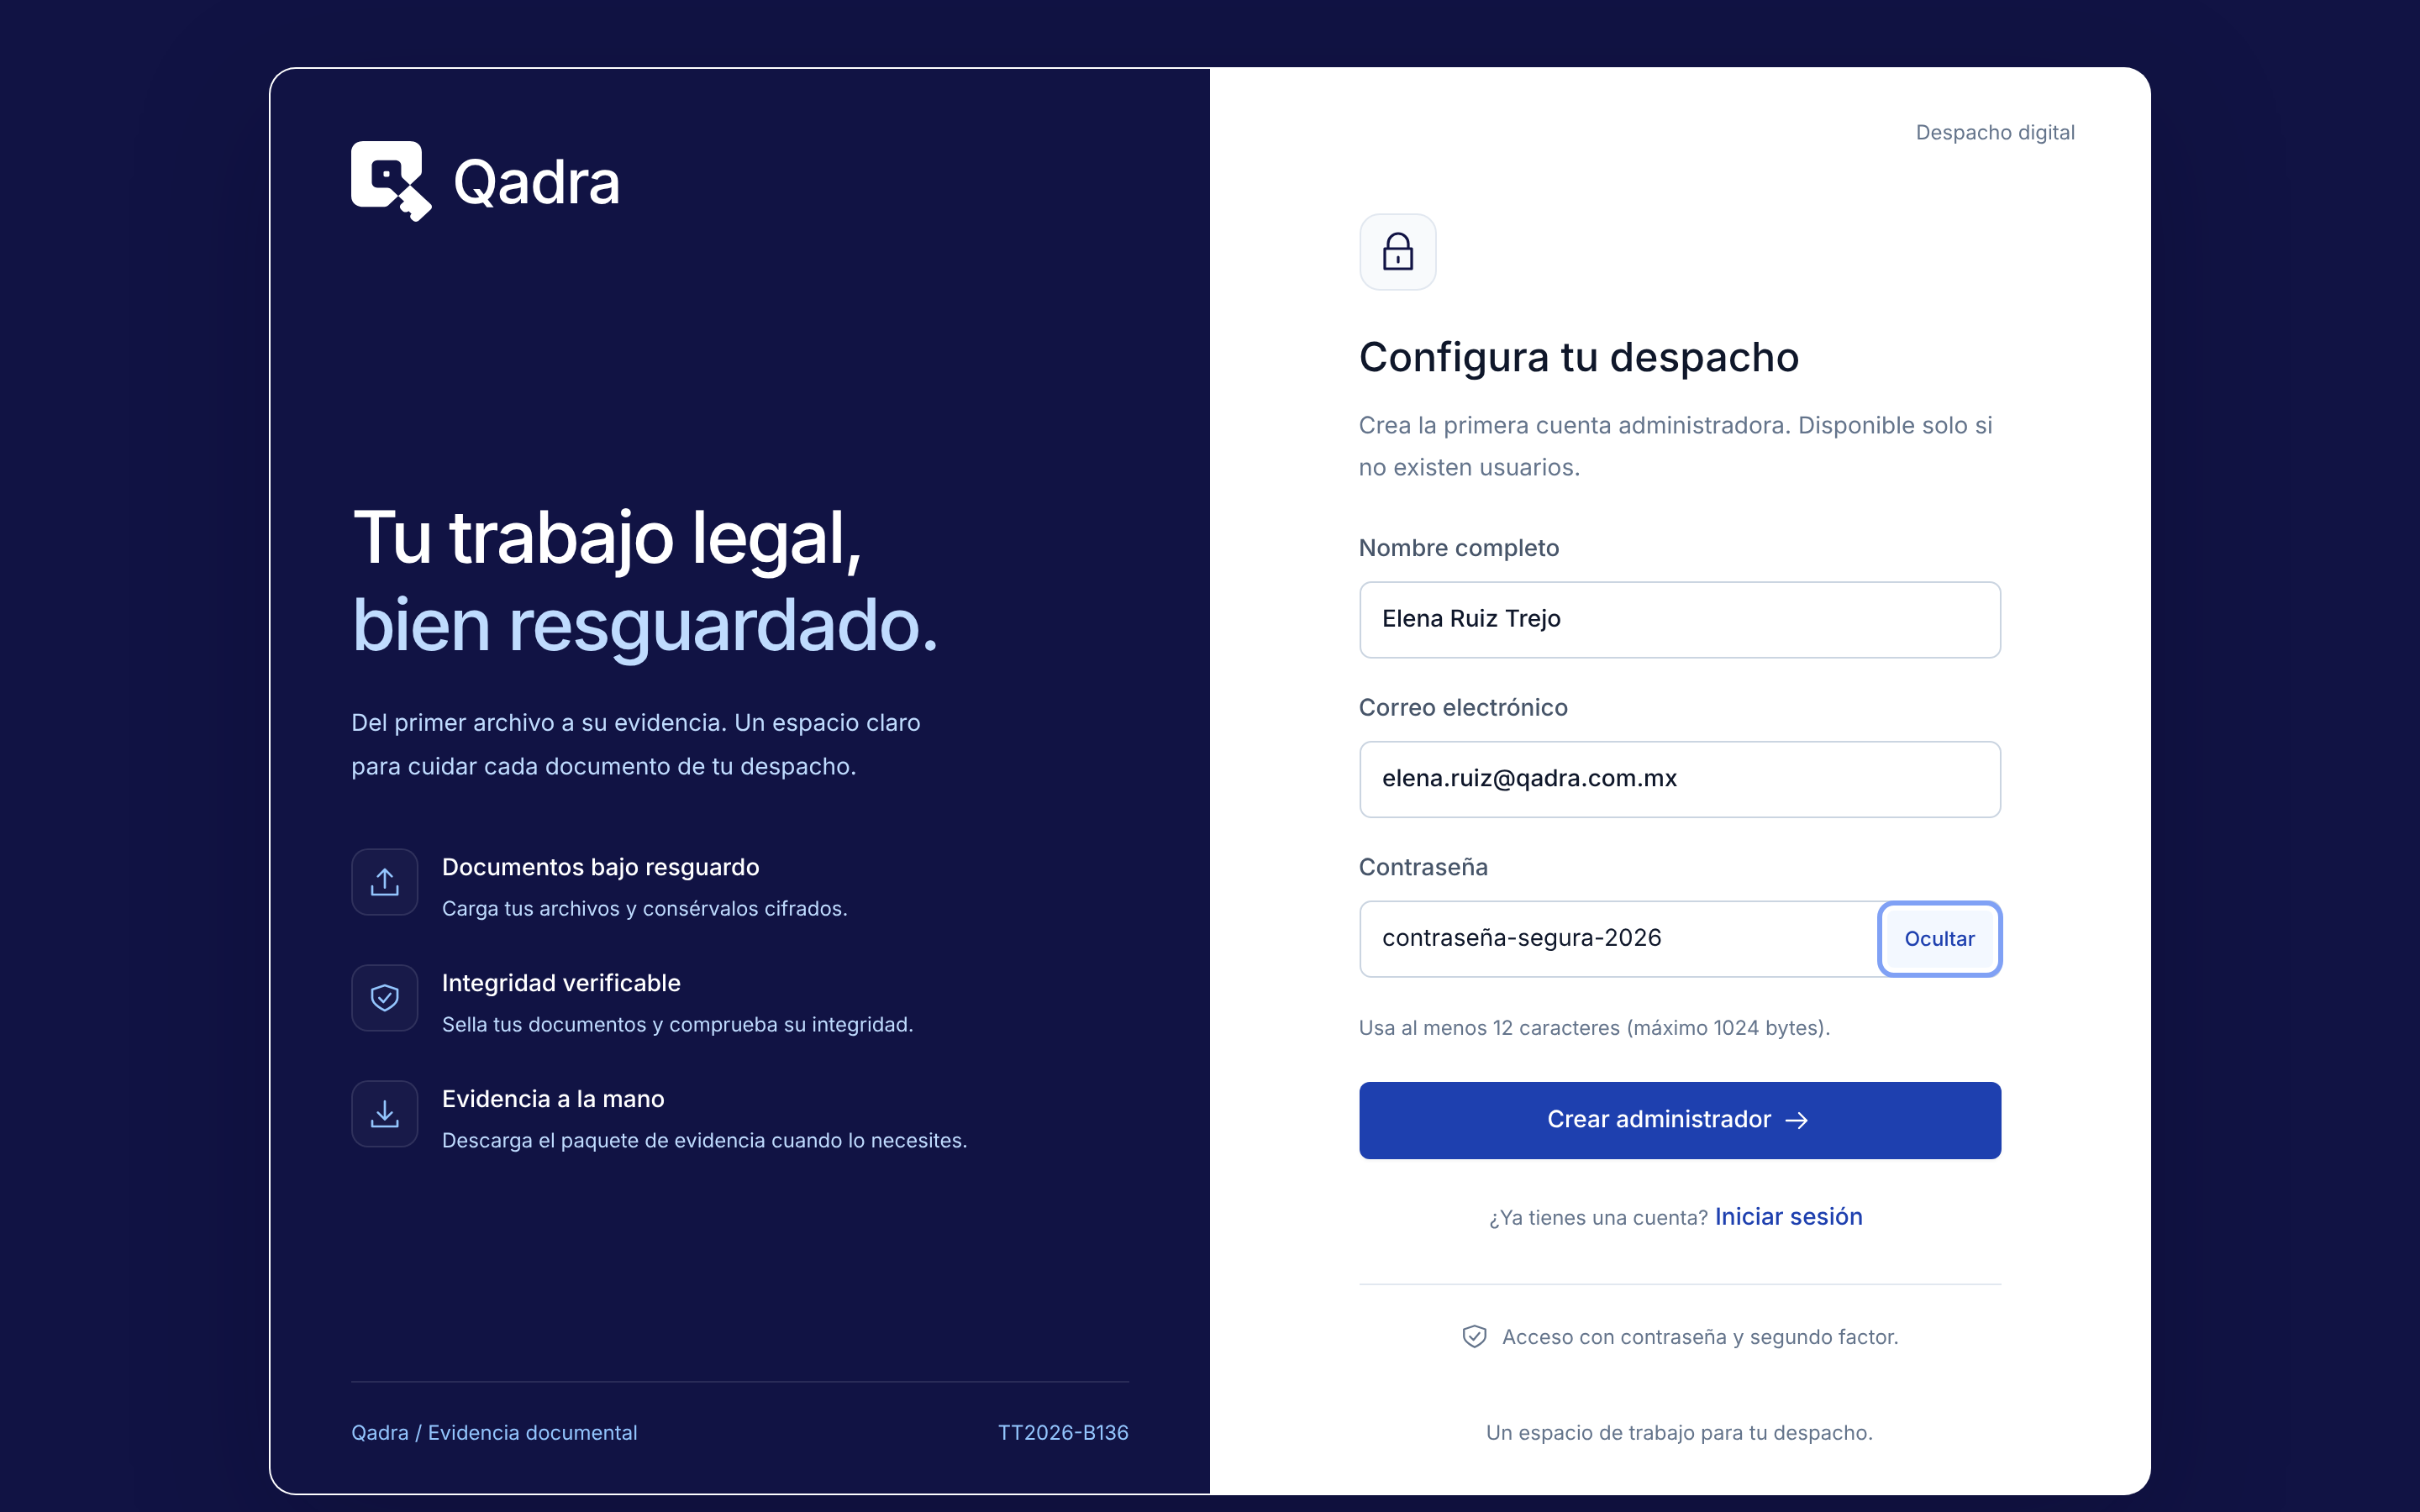
\includegraphics[width=0.9\textwidth]{capturas/A-01-configurar-despacho.png}
  \caption{Creación de la primera cuenta de Administrador.}
  \label{fig:manual-configurar-despacho}
\end{figure}

\begin{figure}[H]
  \centering
  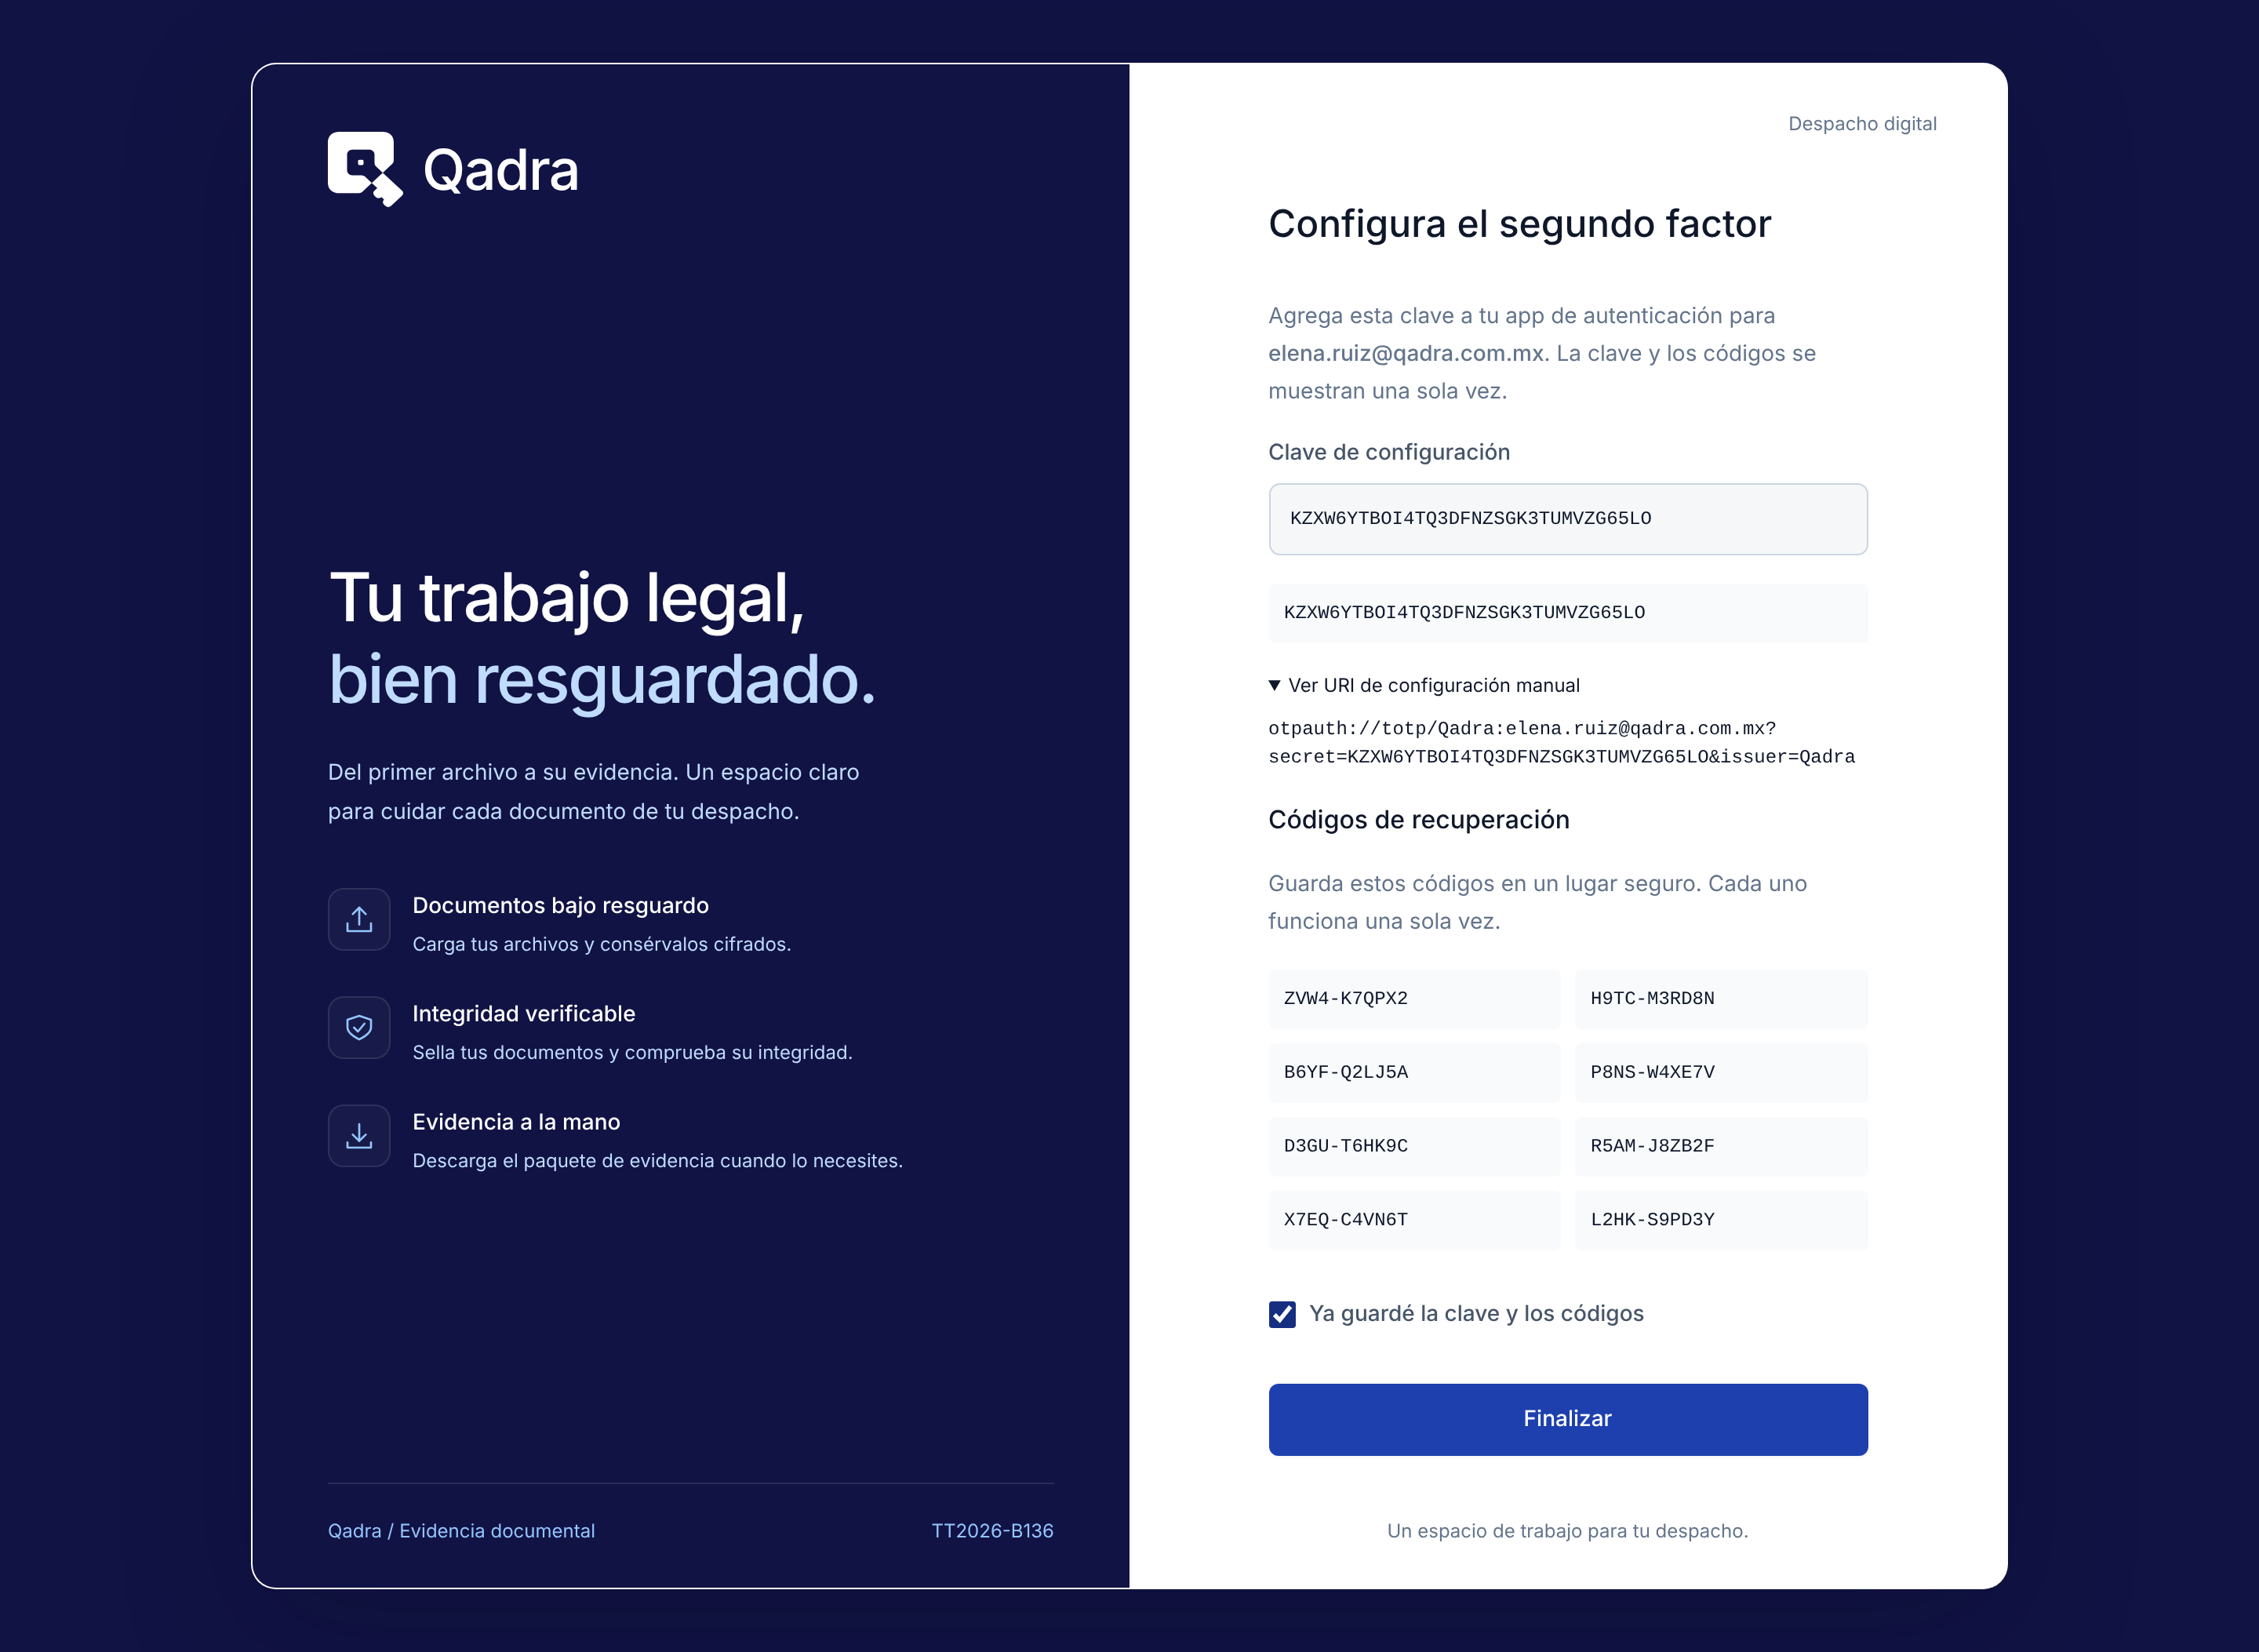
\includegraphics[width=0.9\textwidth]{capturas/A-02-configurar-segundo-factor.png}
  \caption{Configuración del segundo factor y códigos de recuperación.}
  \label{fig:manual-configurar-segundo-factor}
\end{figure}

\resultado La cuenta queda creada y Qadra vuelve a la pantalla de inicio de
sesión. Entre con su correo, su contraseña y su código
(\cref{sec:iniciar-sesion}).

\importante{La clave y los códigos se muestran una sola vez. Guárdelos antes
de hacer clic en \textbf{Finalizar}.}

\nota{Si el despacho ya tiene un Administrador, aparece el mensaje
\enquote{El despacho ya tiene un administrador. Inicia sesión con tu
cuenta.}}

% ---------------------------------------------------------------------
\section{Aceptar una invitación}\label{sec:aceptar-invitacion}

\paraque Crea su cuenta a partir del correo de invitación que le envió el
Administrador.

\disponible Cualquier persona invitada: Litigante, Asistente legal o Cliente.

\pasos
\begin{enumerate}
  \item Abra el enlace del correo de invitación. Aparece la pantalla
        \textbf{Acepta tu invitación}.
  \item En \textbf{Tu contraseña}, escriba la contraseña que usará en Qadra
        (entre 12 y 1024 bytes; en la práctica, al menos 12 caracteres).
  \item Haga clic en \textbf{Preparar segundo factor}.
  \item En la pantalla \textbf{Confirma tu segundo factor}, agregue a su app
        de autenticación la clave que se muestra. Si su app pide un enlace,
        abra \textbf{Enlace para tu autenticador}.
  \item Guarde en un lugar privado los códigos de recuperación de la lista.
  \item Marque la casilla \textbf{Ya guardé mis códigos de recuperación}.
  \item Escriba de nuevo su contraseña en \textbf{Tu contraseña} y el
        \textbf{Código de 6 dígitos} que muestra su app.
  \item Haga clic en \textbf{Confirmar alta}.
\end{enumerate}

\begin{figure}[H]
  \centering
  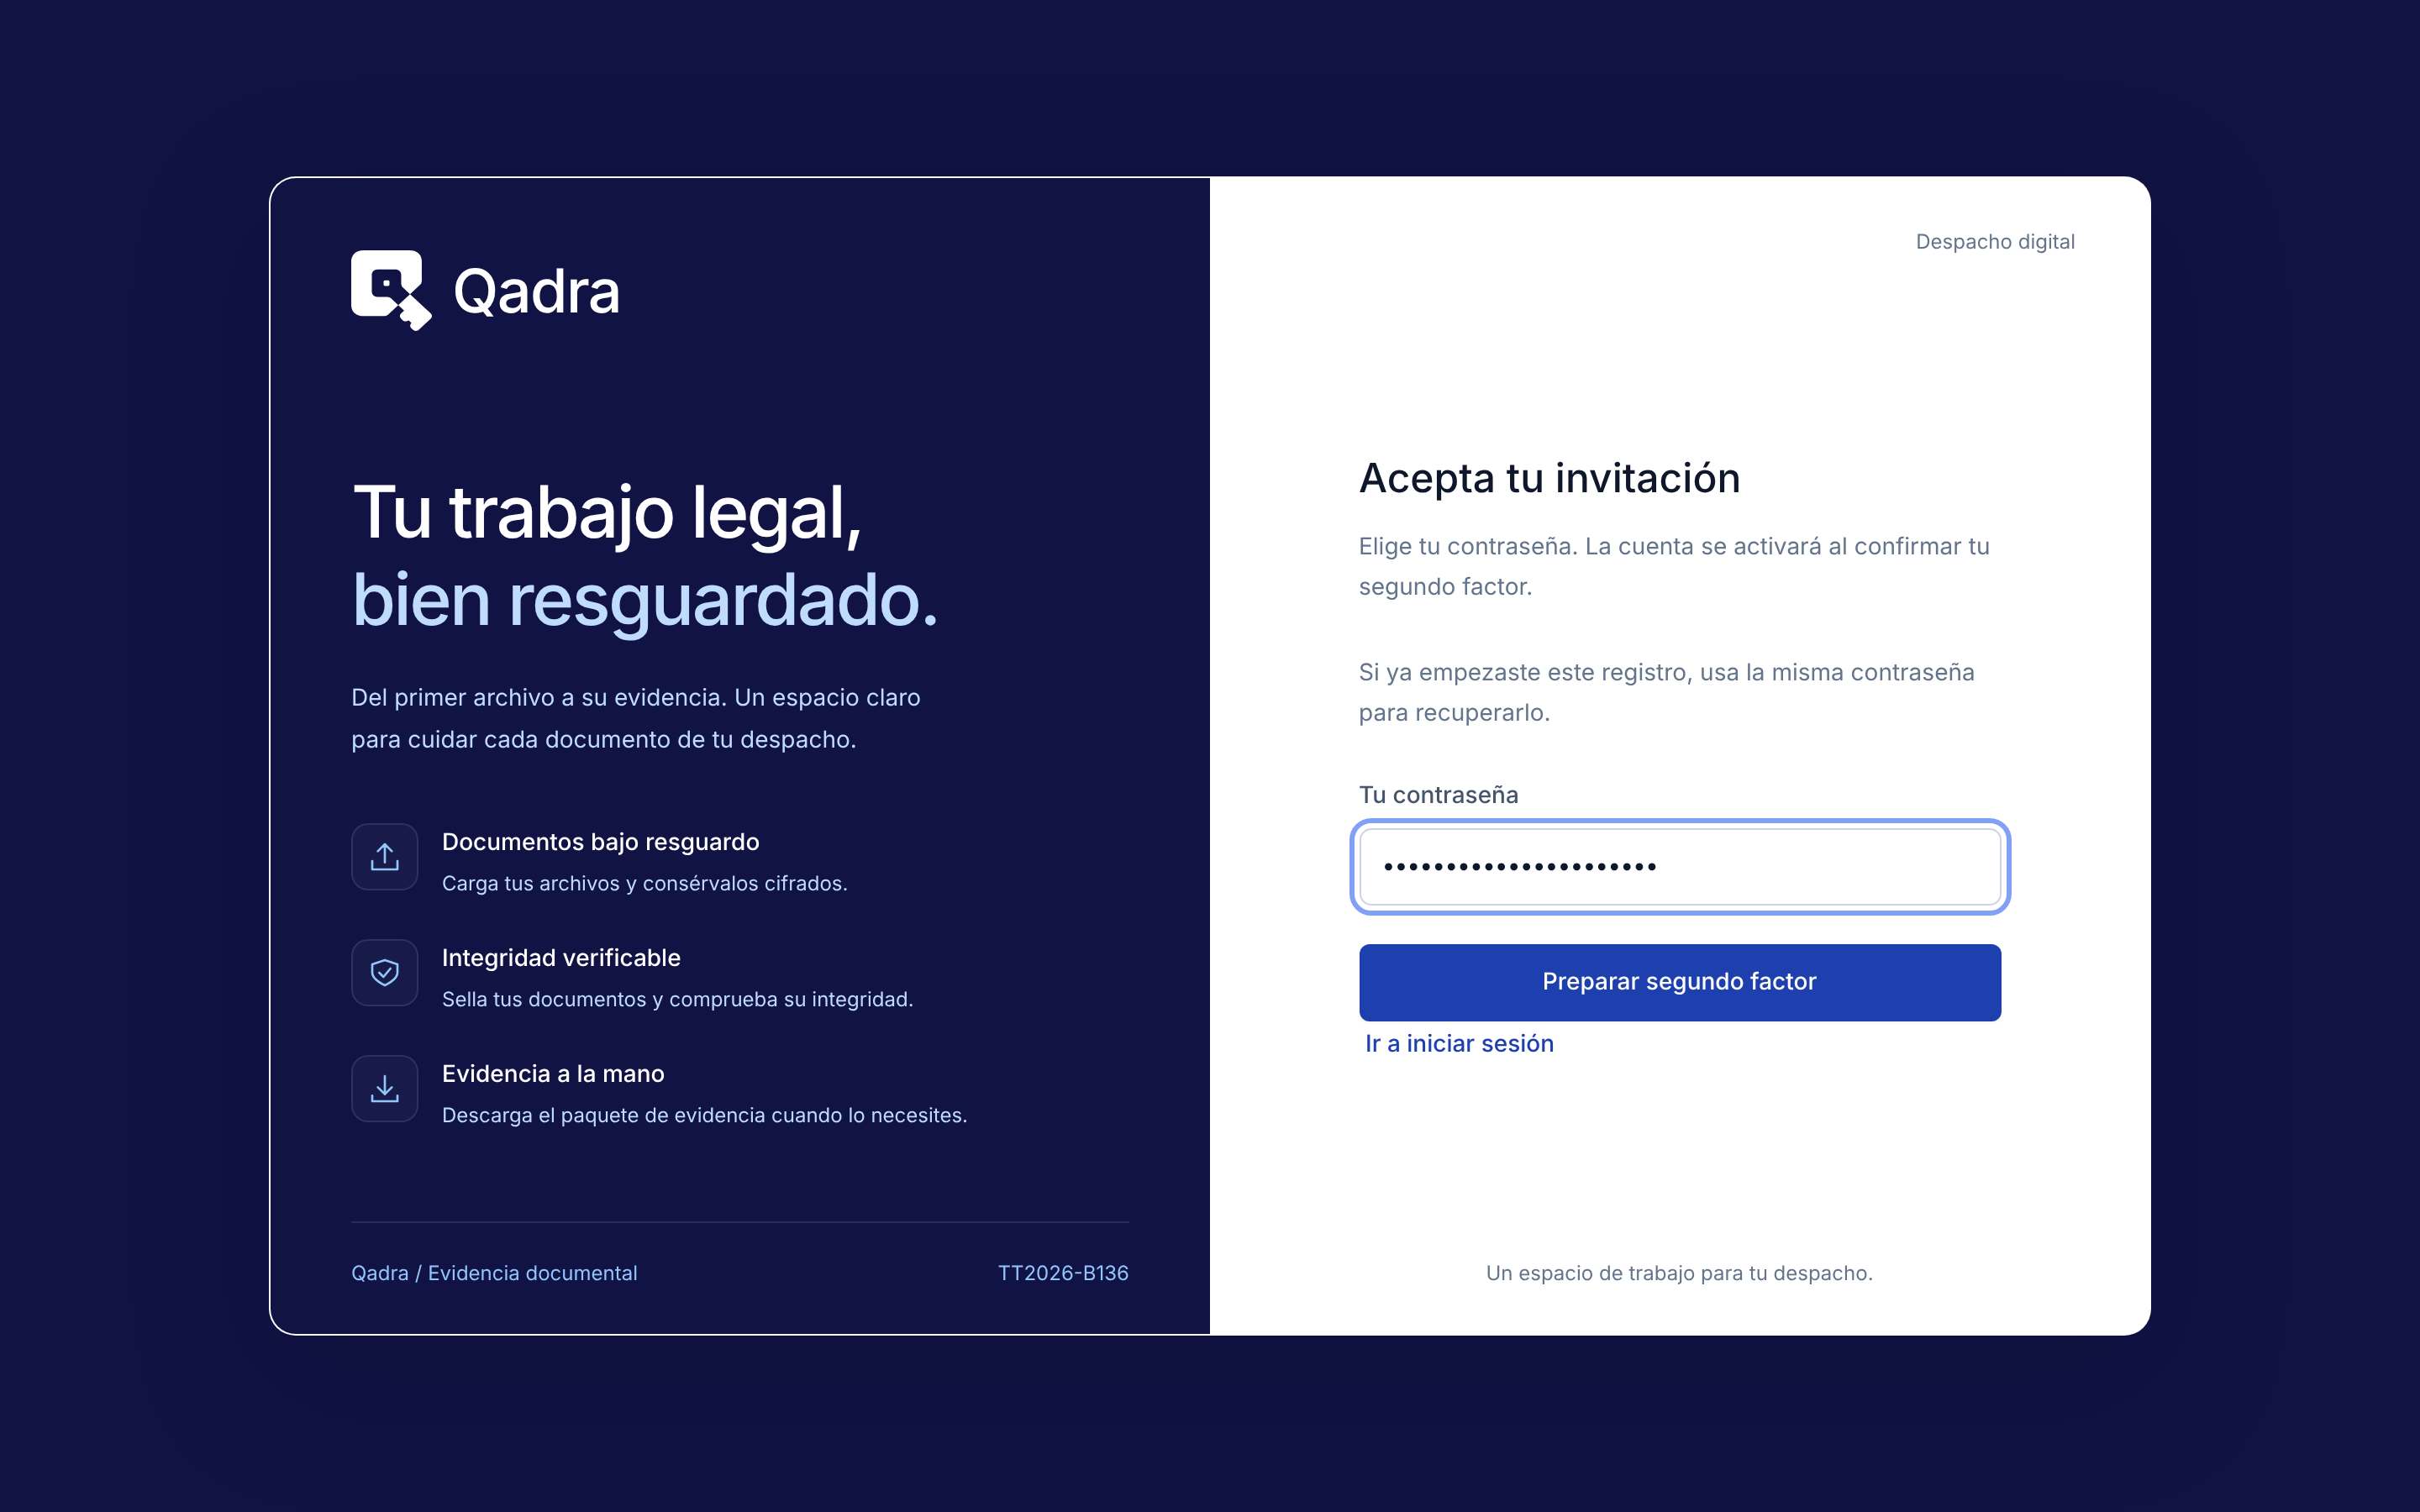
\includegraphics[width=0.9\textwidth]{capturas/A-03-aceptar-invitacion.png}
  \caption{Inicio del alta desde una invitación.}
  \label{fig:manual-aceptar-invitacion}
\end{figure}

\begin{figure}[H]
  \centering
  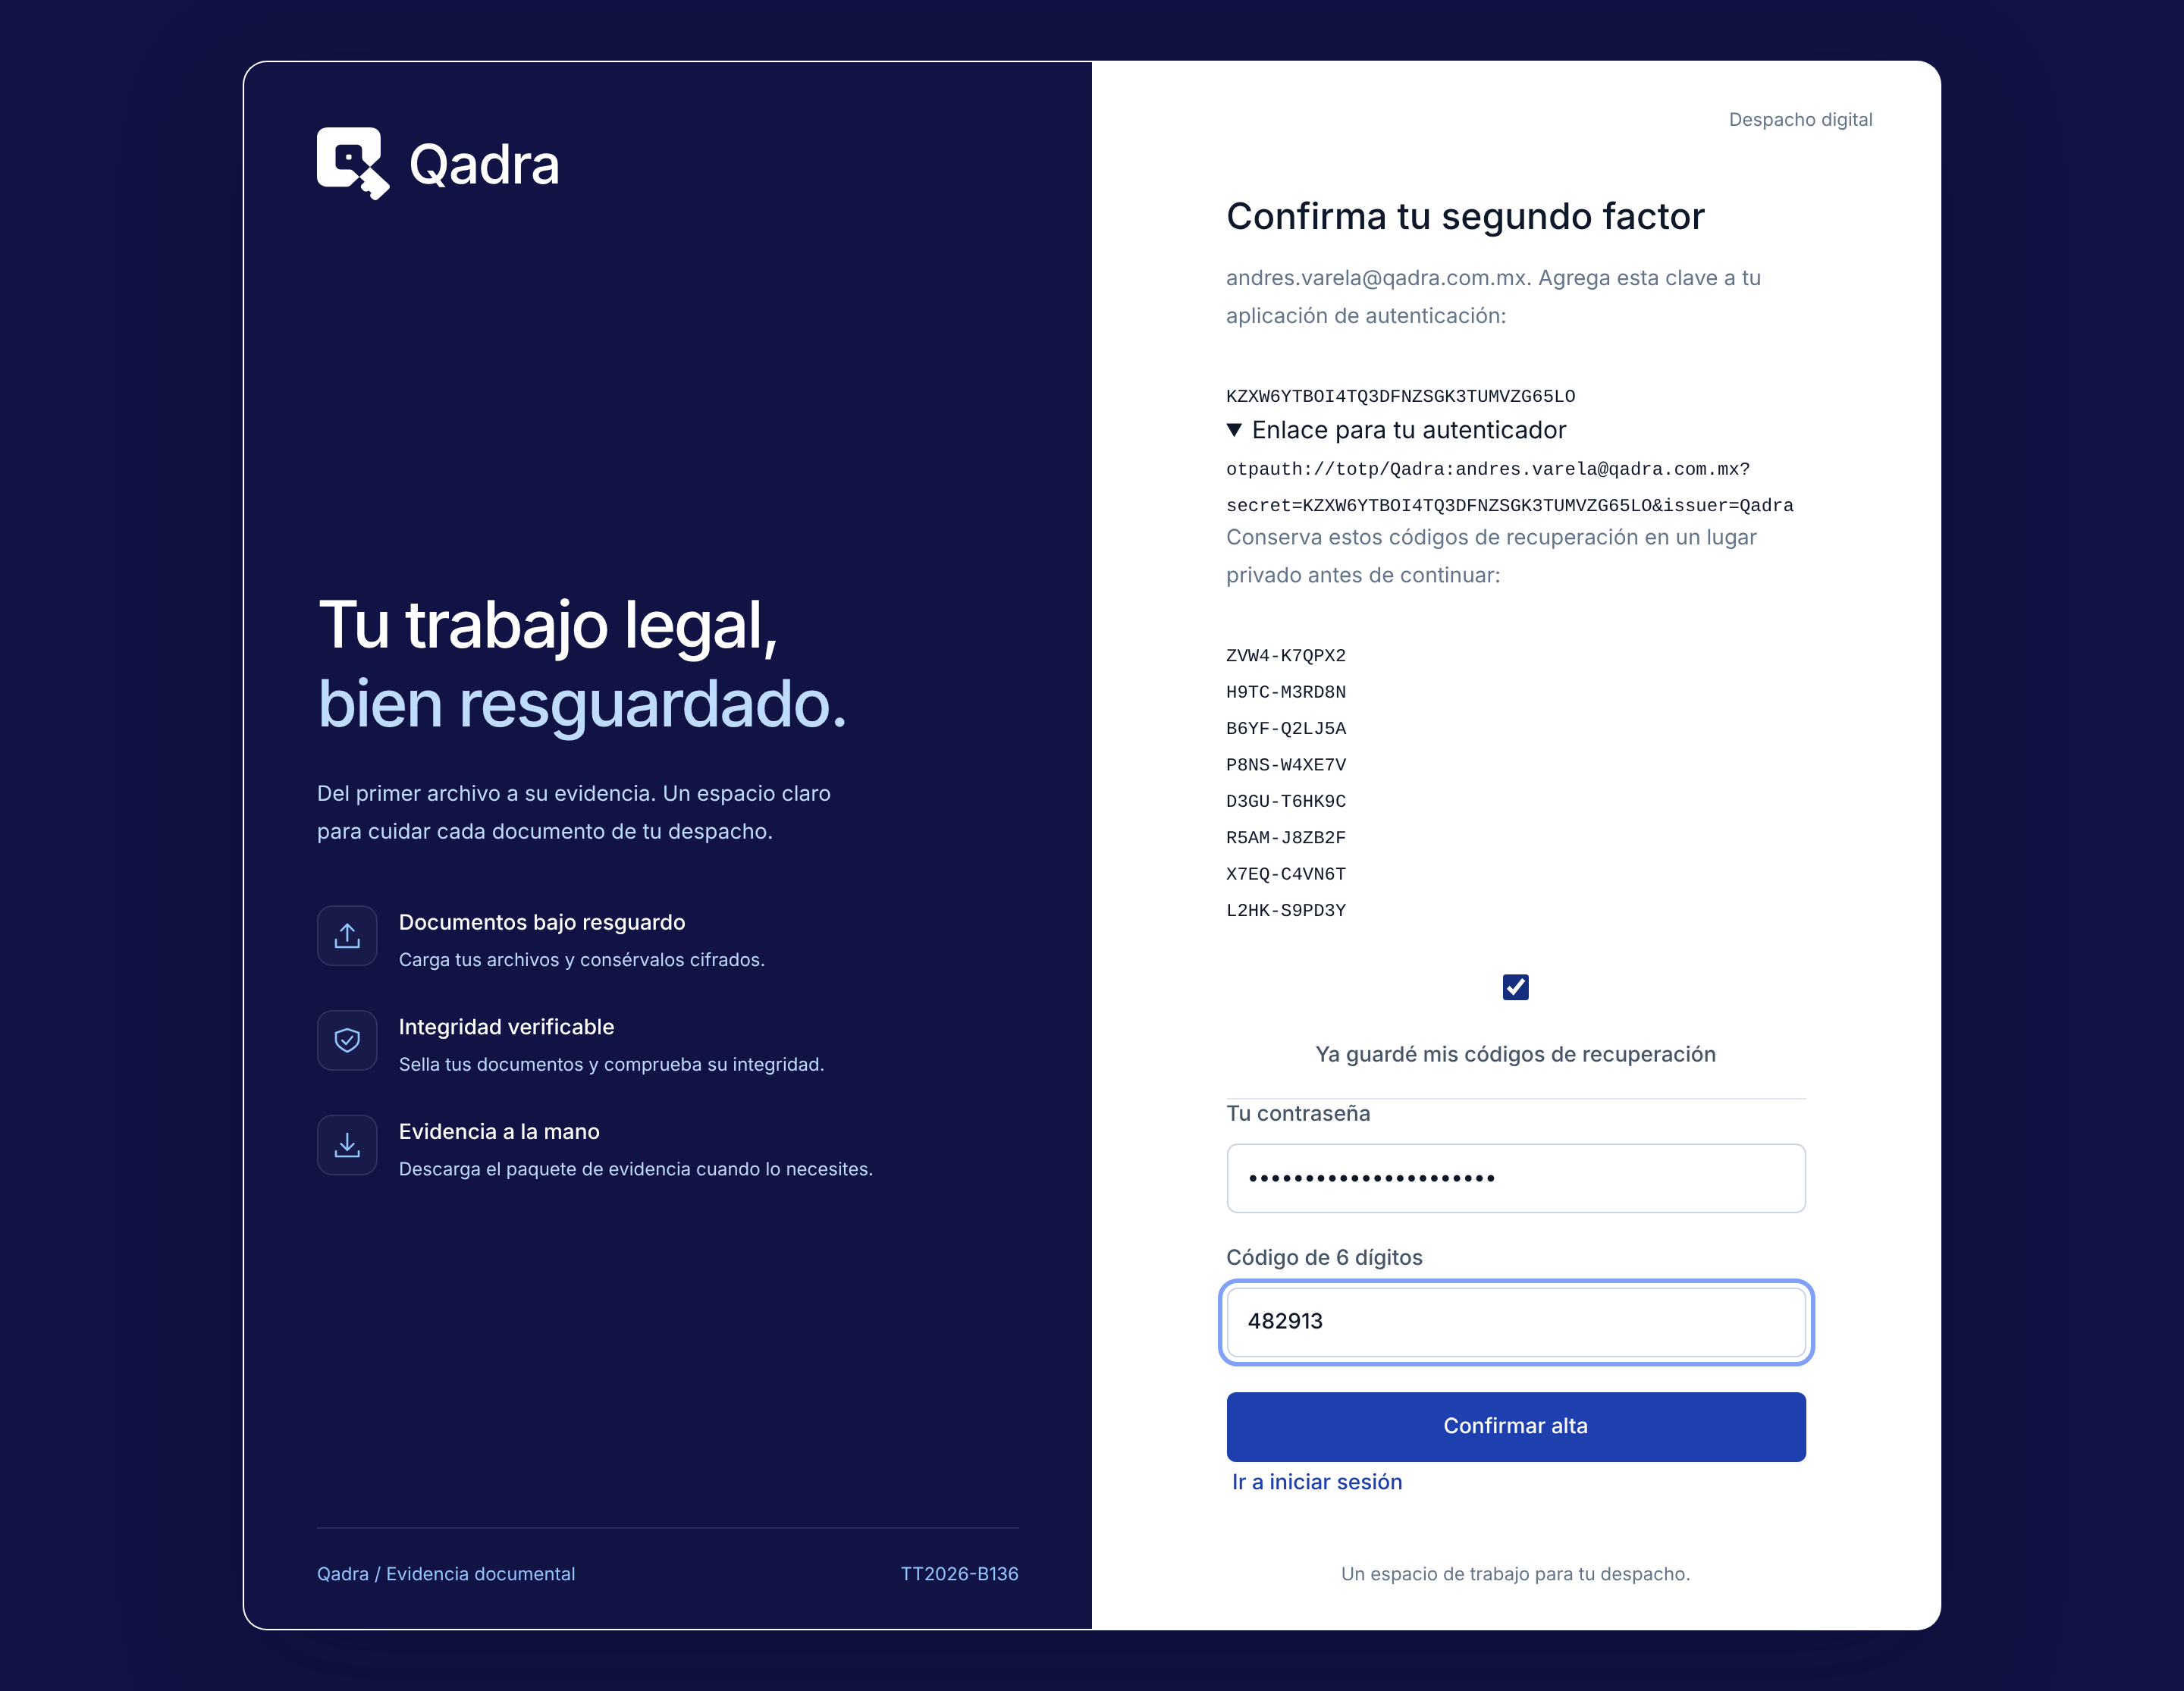
\includegraphics[width=0.9\textwidth]{capturas/A-04-confirmar-segundo-factor.png}
  \caption{Confirmación del segundo factor durante el alta.}
  \label{fig:manual-confirmar-segundo-factor}
\end{figure}

\resultado Aparece \enquote{Cuenta creada: [correo]. Ya puedes iniciar sesión
con tu contraseña y segundo factor.} Haga clic en
\textbf{Ir a iniciar sesión}.

\begin{itemize}
  \item \textbf{Si el alta se interrumpió:} abra de nuevo el mismo enlace.
        Qadra le pide \enquote{Comprueba si tu alta terminó antes de
        repetirla.} Escriba la misma contraseña y haga clic en
        \textbf{Comprobar resultado}.
  \item \textbf{Si el enlace no funciona:} aparece \enquote{El enlace no es
        válido. Abre el correo original o solicita un reenvío al
        administrador.}
  \item \textbf{Si el navegador no puede guardar el intento:} se le pide
        conservar la pestaña abierta hasta confirmar el alta. No la cierre.
\end{itemize}

% ---------------------------------------------------------------------
\section{Iniciar sesión}\label{sec:iniciar-sesion}

\paraque Permite entrar a Qadra con su correo, su contraseña y el código de
su app de autenticación.

\disponible Todos los roles con cuenta.

\pasos
\begin{enumerate}
  \item Abra Qadra en su navegador. Aparece la pantalla
        \textbf{Accede a tu despacho}.
  \item Ingrese su \textbf{Correo electrónico} y su \textbf{Contraseña}.
        Para revisar lo que escribió, haga clic en \textbf{Mostrar}.
  \item Haga clic en \textbf{Continuar}.
  \item En la pantalla \textbf{Un paso más}, abra su app de autenticación y
        escriba el \textbf{Código de 6 dígitos}.
  \item Haga clic en \textbf{Verificar y entrar}.
\end{enumerate}

\begin{figure}[H]
  \centering
  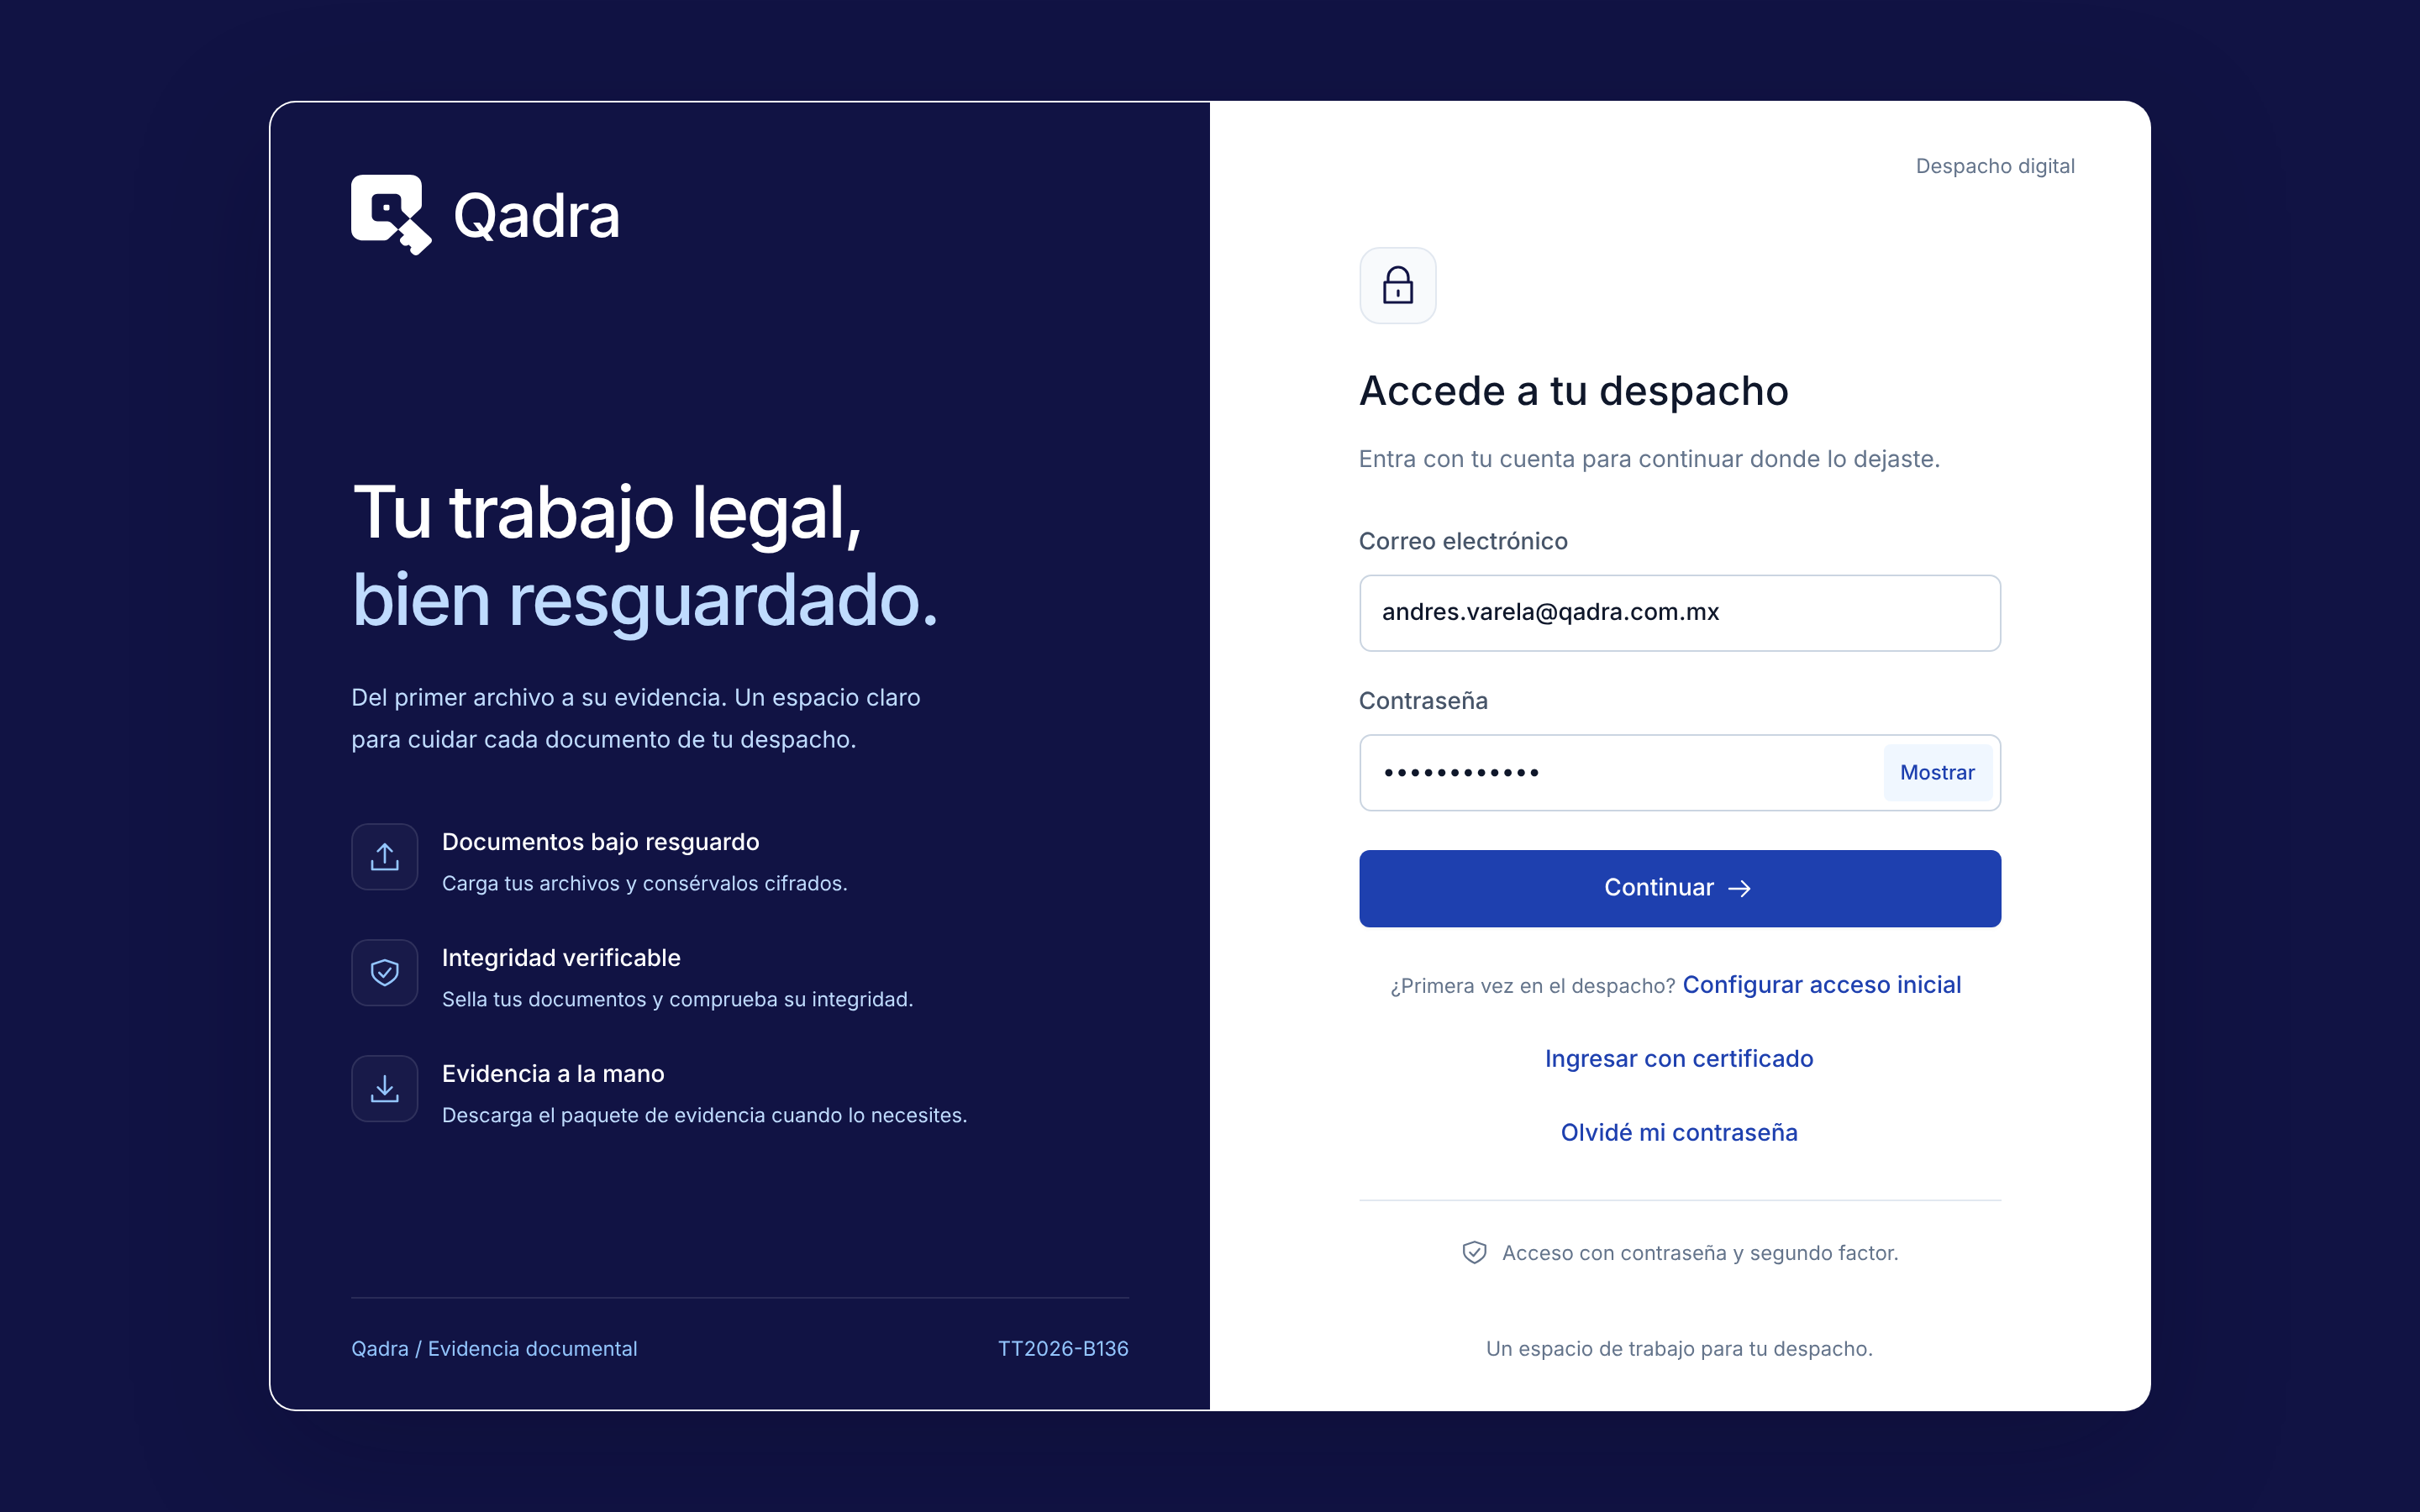
\includegraphics[width=0.9\textwidth]{capturas/A-05-inicio-sesion.png}
  \caption{Inicio de sesión con correo y contraseña.}
  \label{fig:manual-inicio-sesion}
\end{figure}

\begin{figure}[H]
  \centering
  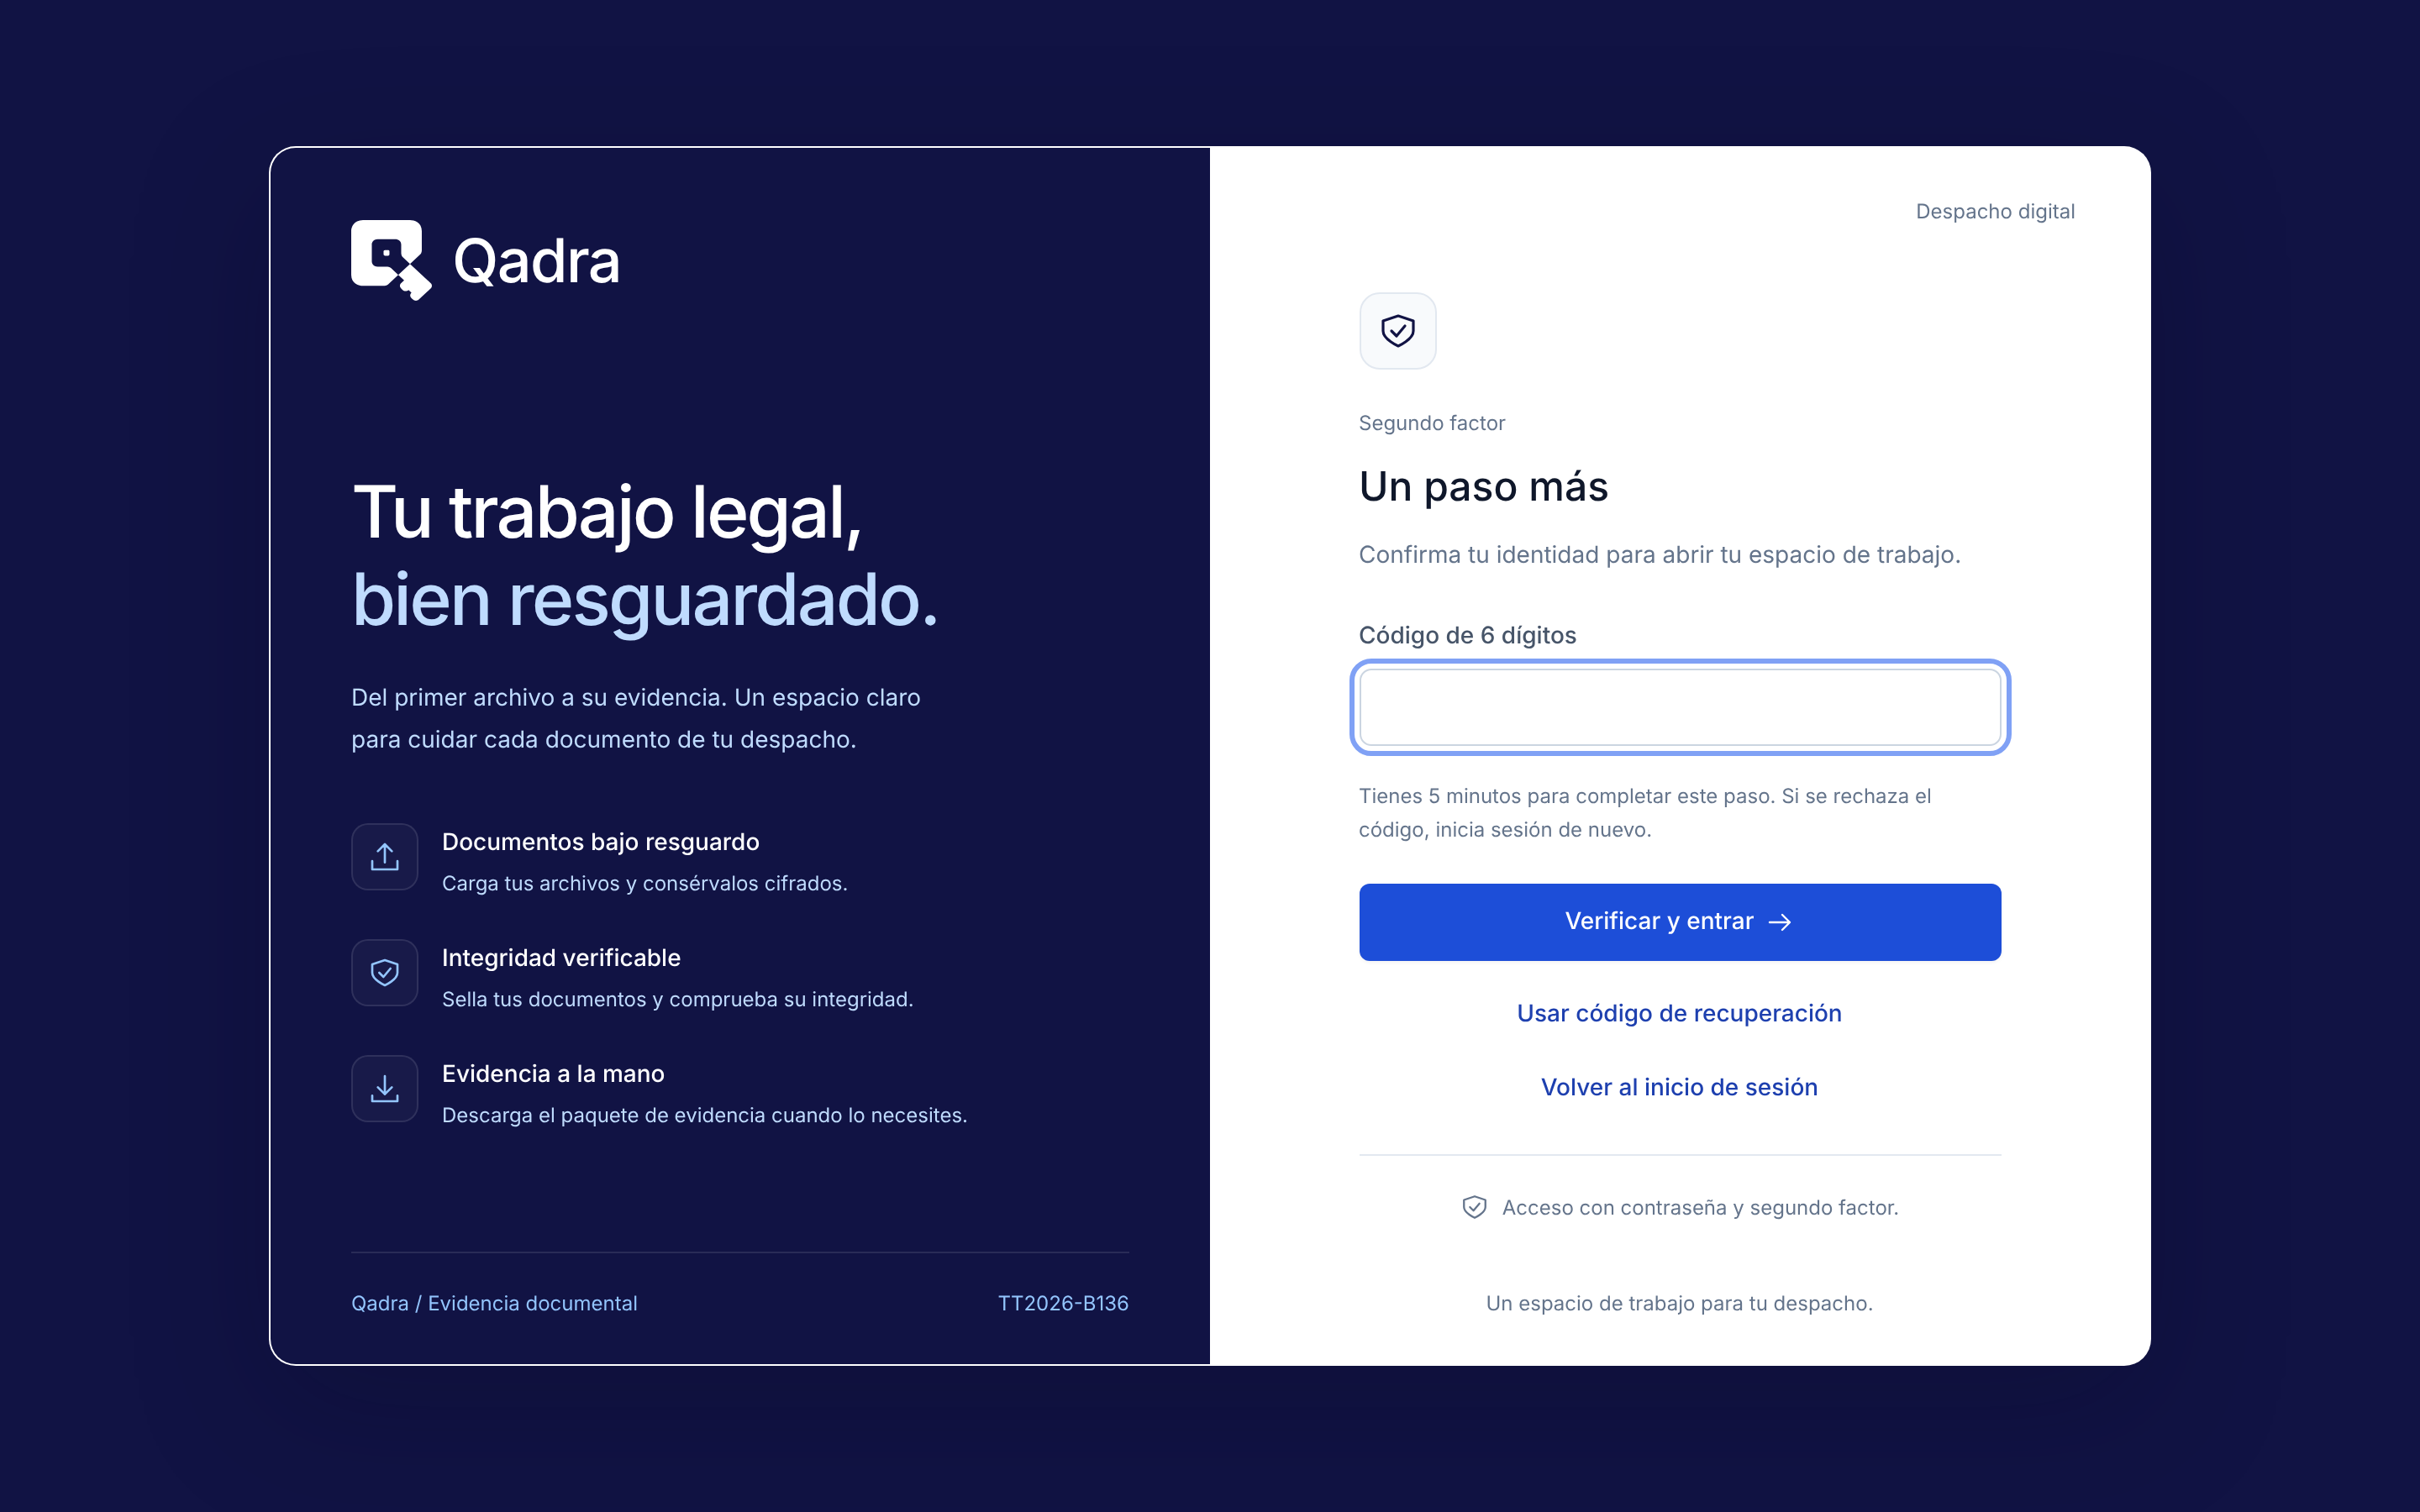
\includegraphics[width=0.9\textwidth]{capturas/A-06-segundo-factor.png}
  \caption{Confirmación con el segundo factor.}
  \label{fig:manual-segundo-factor}
\end{figure}

\resultado Se abre su espacio de trabajo. El Administrador, el Litigante y el
Asistente legal llegan a \textbf{Inicio}; el Cliente llega a
\textbf{Mis contratos}.

\begin{itemize}
  \item La pantalla indica el tiempo disponible para escribir el código:
        \enquote{Tienes 5 minutos para completar este paso. Si se rechaza el código, inicia
        sesión de nuevo.}
  \item Si el código se rechaza, aparece \enquote{El código fue rechazado o
        venció. Vuelve a iniciar sesión.} Empiece de nuevo desde el paso 1.
  \item Después de varios intentos fallidos aparece \enquote{Demasiados
        intentos. Espera 15 minutos antes de volver a intentarlo.}
\end{itemize}

% ---------------------------------------------------------------------
\section{Entrar con un código de recuperación}\label{sec:codigo-recuperacion}

\paraque Permite entrar cuando no tiene a la mano su app de autenticación.

\disponible Todos los roles con cuenta.

\pasos
\begin{enumerate}
  \item Siga los pasos 1 a 3 de la \cref{sec:iniciar-sesion}.
  \item En la pantalla \textbf{Un paso más}, haga clic en
        \textbf{Usar código de recuperación}.
  \item Escriba uno de sus códigos en \textbf{Código de recuperación}.
  \item Haga clic en \textbf{Verificar y entrar}.
\end{enumerate}

\resultado Entra a Qadra como en un inicio de sesión normal.

\nota{Cada código funciona una sola vez; táchelo de su lista después de
usarlo. Si ya no conserva ningún código, contacte al Administrador. Para
volver al código de su app, haga clic en \textbf{Usar app de autenticación}.}

% ---------------------------------------------------------------------
\section{Recuperar la contraseña}\label{sec:recuperar-contrasena}

\paraque Permite elegir una contraseña nueva si olvidó la anterior. Su
segundo factor no cambia.

\disponible Todos los roles con cuenta.

\pasos
\begin{enumerate}
  \item En la pantalla de inicio de sesión, haga clic en
        \textbf{Olvidé mi contraseña}.
  \item En \textbf{Recupera tu acceso.}, ingrese su
        \textbf{Correo electrónico} y haga clic en
        \textbf{Solicitar enlace}.
  \item Abra el enlace que llegue a su correo.
  \item En \textbf{Elige una nueva contraseña.}, escriba la
        \textbf{Nueva contraseña} y repítala en
        \textbf{Repite la nueva contraseña}. Use al menos 12 caracteres y no
        reutilice la anterior.
  \item Haga clic en \textbf{Cambiar contraseña}.
\end{enumerate}

\begin{figure}[H]
  \centering
  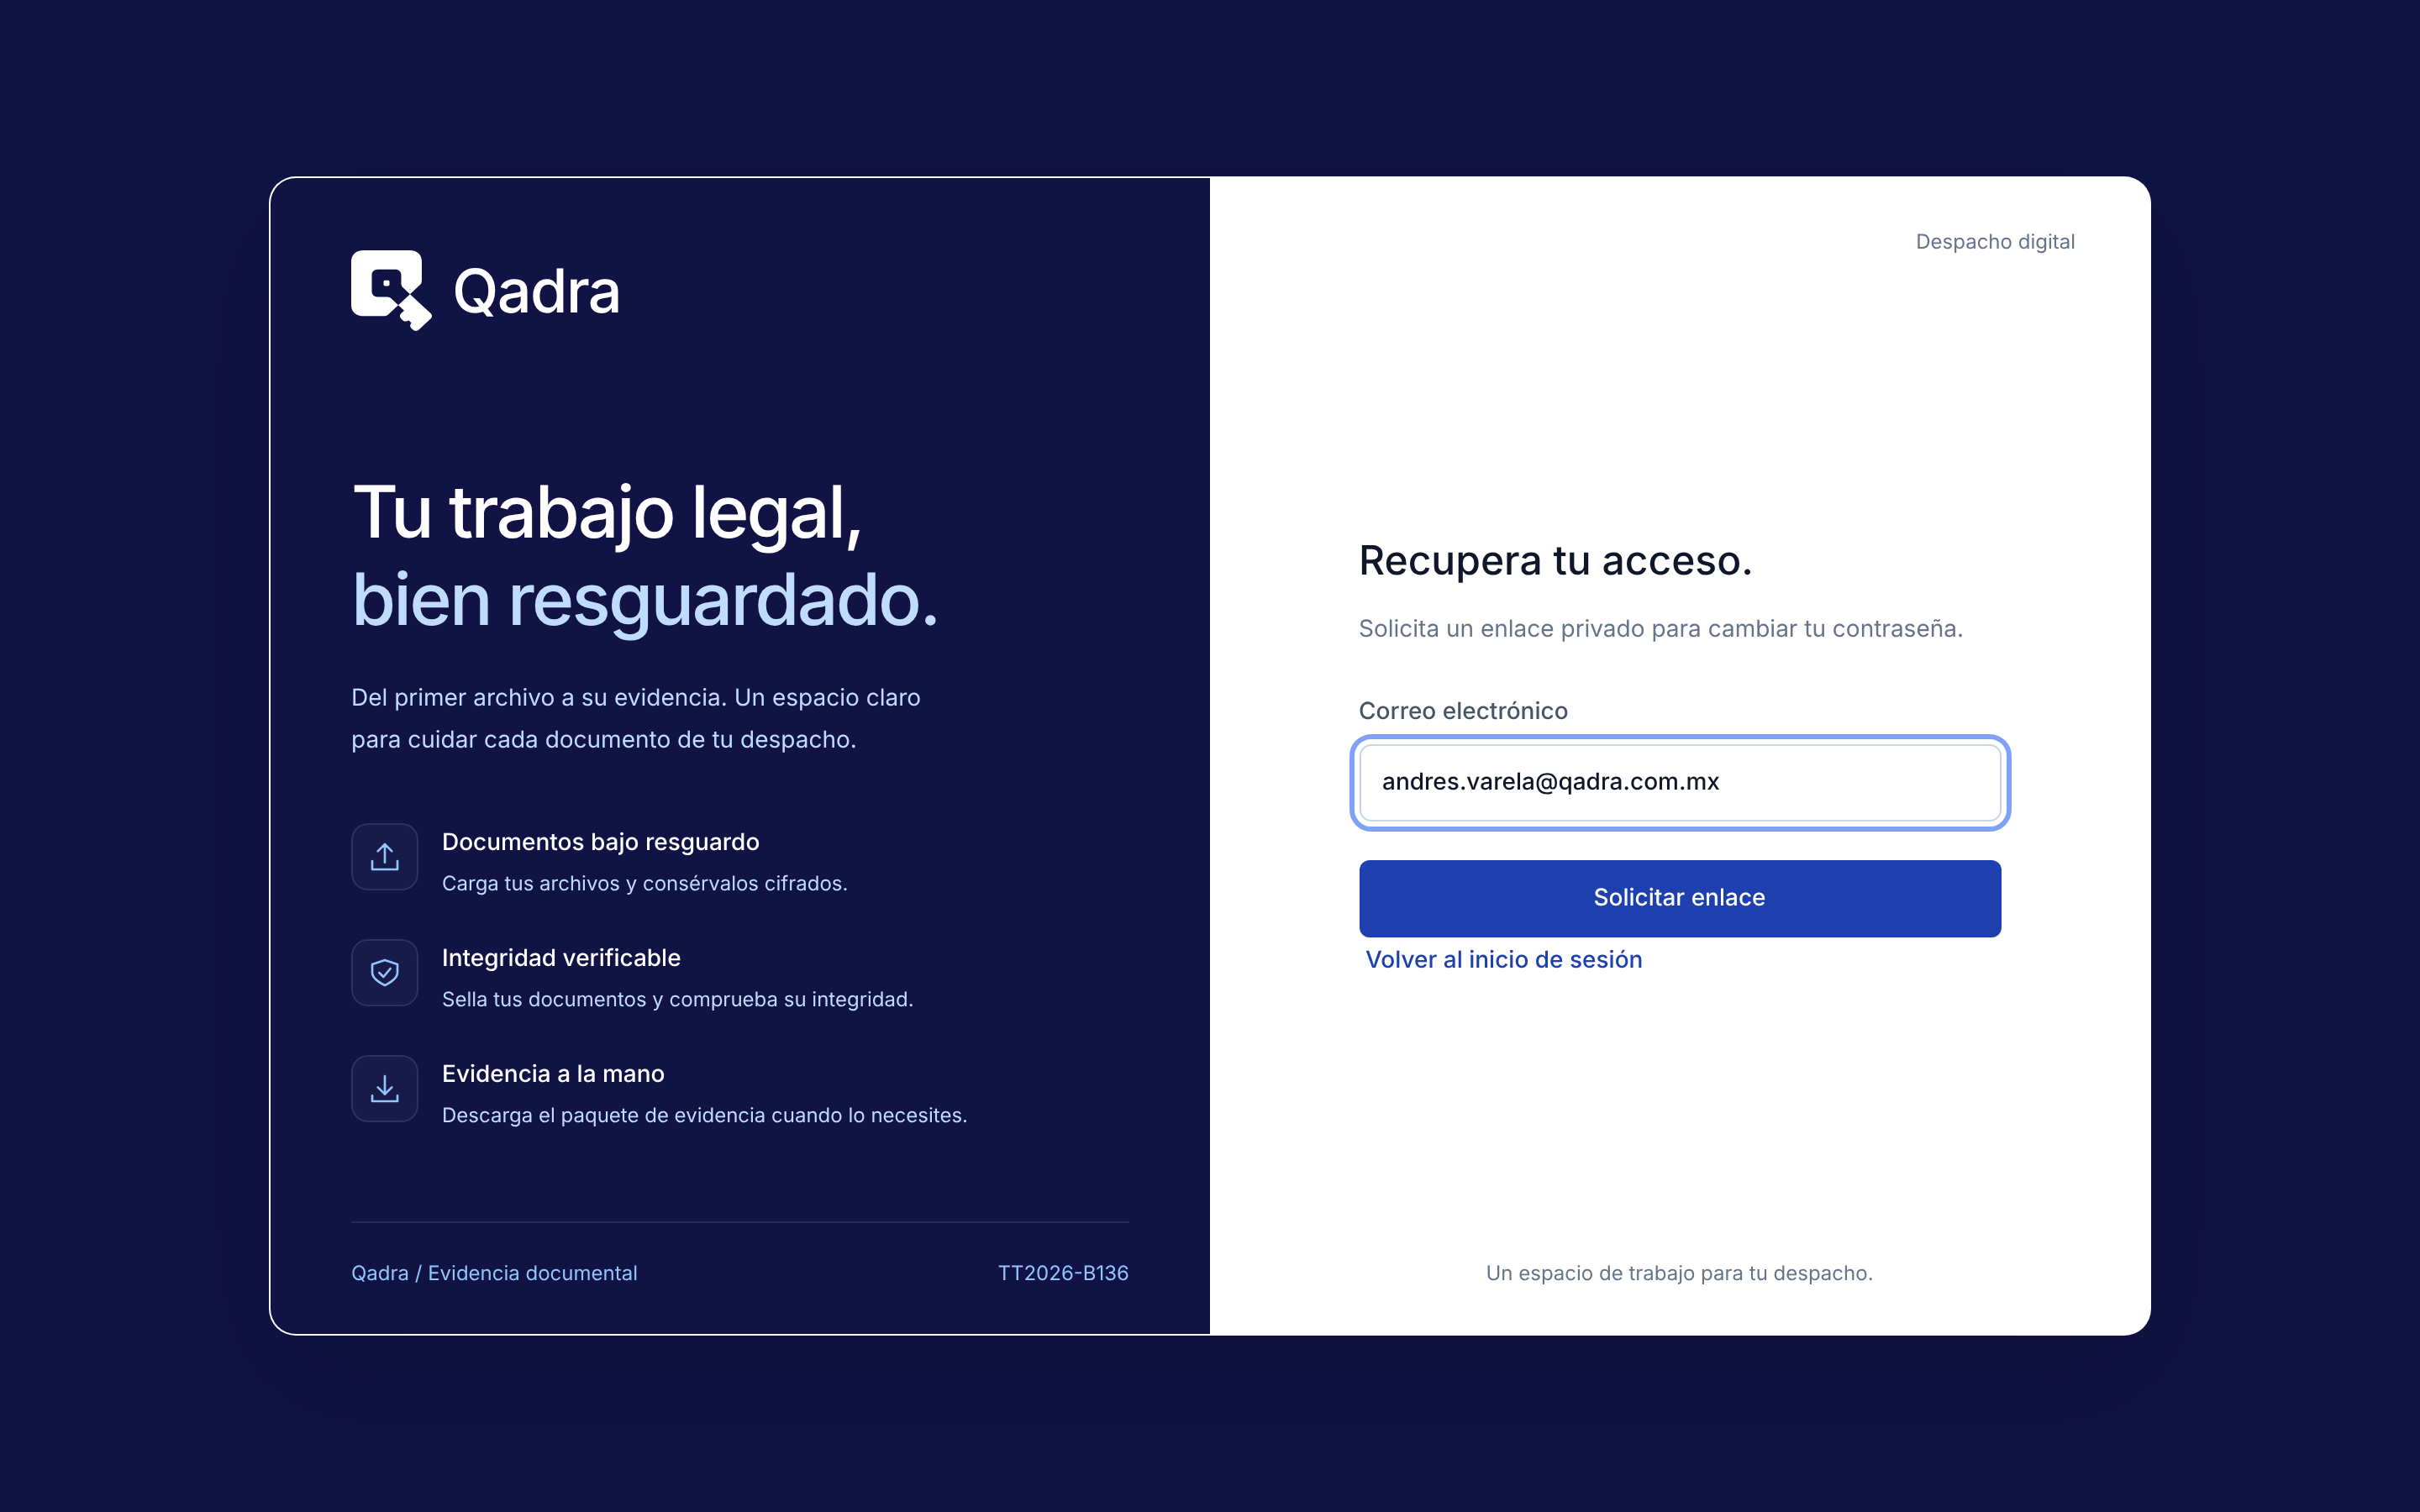
\includegraphics[width=0.9\textwidth]{capturas/A-07-recuperar-acceso.png}
  \caption{Solicitud del enlace de recuperación.}
  \label{fig:manual-recuperar-acceso}
\end{figure}

\begin{figure}[H]
  \centering
  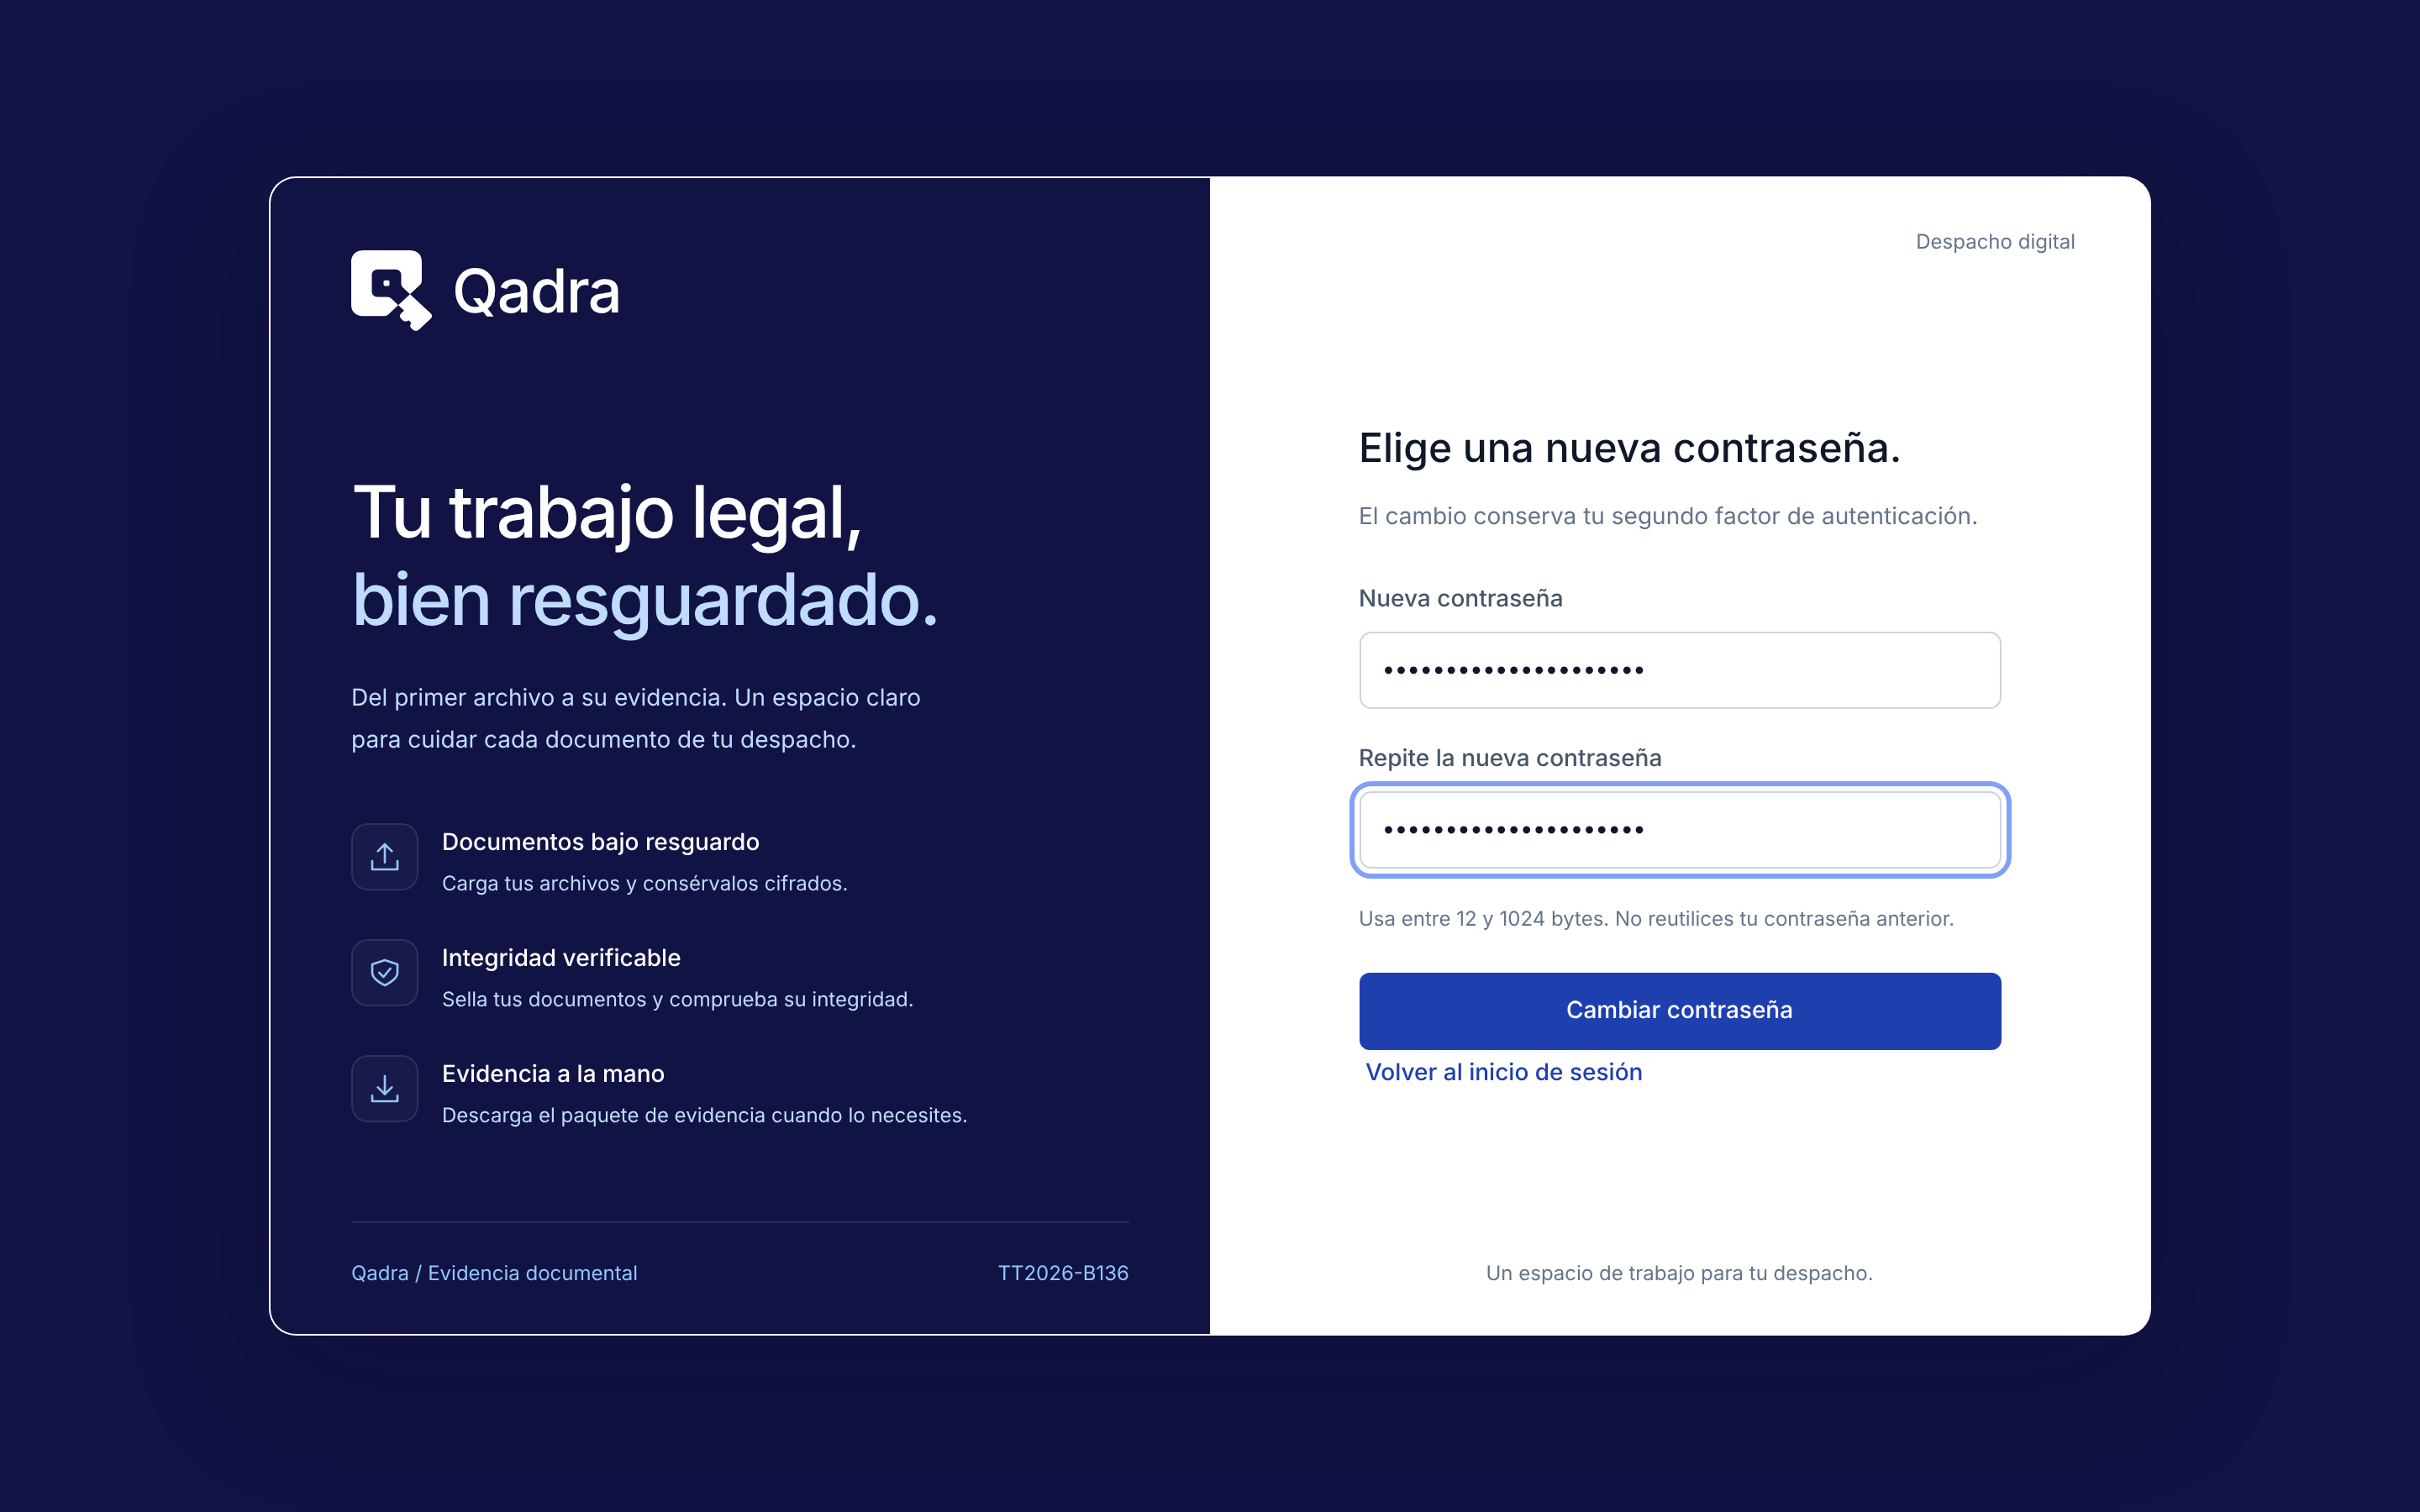
\includegraphics[width=0.9\textwidth]{capturas/A-08-nueva-contrasena.png}
  \caption{Cambio de contraseña desde el enlace.}
  \label{fig:manual-nueva-contrasena}
\end{figure}

\resultado Aparece \enquote{Contraseña actualizada. Inicia sesión con la nueva
contraseña.} Haga clic en \textbf{Volver al inicio de sesión}.

\begin{itemize}
  \item Al solicitar el enlace siempre aparece \enquote{Si la solicitud puede
        atenderse, podrás recibir un enlace. Esta respuesta no confirma un
        envío.} Si no llega ningún correo, revise la dirección escrita o
        contacte al Administrador.
  \item Si el enlace ya se usó o venció, aparece \enquote{El enlace ya no
        puede usarse. Solicita uno nuevo desde el inicio de sesión.}
\end{itemize}

% ---------------------------------------------------------------------
\section{Ingresar con certificado}\label{sec:ingresar-certificado}

\paraque Permite al Administrador entrar con su certificado en lugar de su
contraseña. Después se pide igualmente el segundo factor.

\disponible Administrador, con un certificado vinculado previamente en
\textbf{Mi firma digital}, pestaña \textbf{Acceso con certificado}.

Tenga a la mano: el recibo del vínculo (archivo \texttt{.json}), su clave
privada cifrada (archivo \texttt{.pem}) y la contraseña de esa clave.

\pasos
\begin{enumerate}
  \item En la pantalla de inicio de sesión, haga clic en
        \textbf{Ingresar con certificado}.
  \item En \textbf{Ingresa con tu certificado.}, seleccione su archivo en
        \textbf{Recibo público del vínculo}. Revise que el nombre y la huella
        mostrados sean los suyos.
  \item Haga clic en \textbf{Preparar acceso}.
  \item En \textbf{Firmar en este dispositivo}, seleccione su
        \textbf{Clave privada cifrada} y escriba la
        \textbf{Contraseña de la clave}. Si se solicita, seleccione también
        su certificado en \textbf{Certificado para firma local}.
  \item Haga clic en \textbf{Firmar localmente}.
  \item Haga clic en \textbf{Comprobar firma}.
  \item Escriba el \textbf{Código de 6 dígitos} de su app y haga clic en
        \textbf{Verificar y entrar}.
\end{enumerate}

\begin{figure}[H]
  \centering
  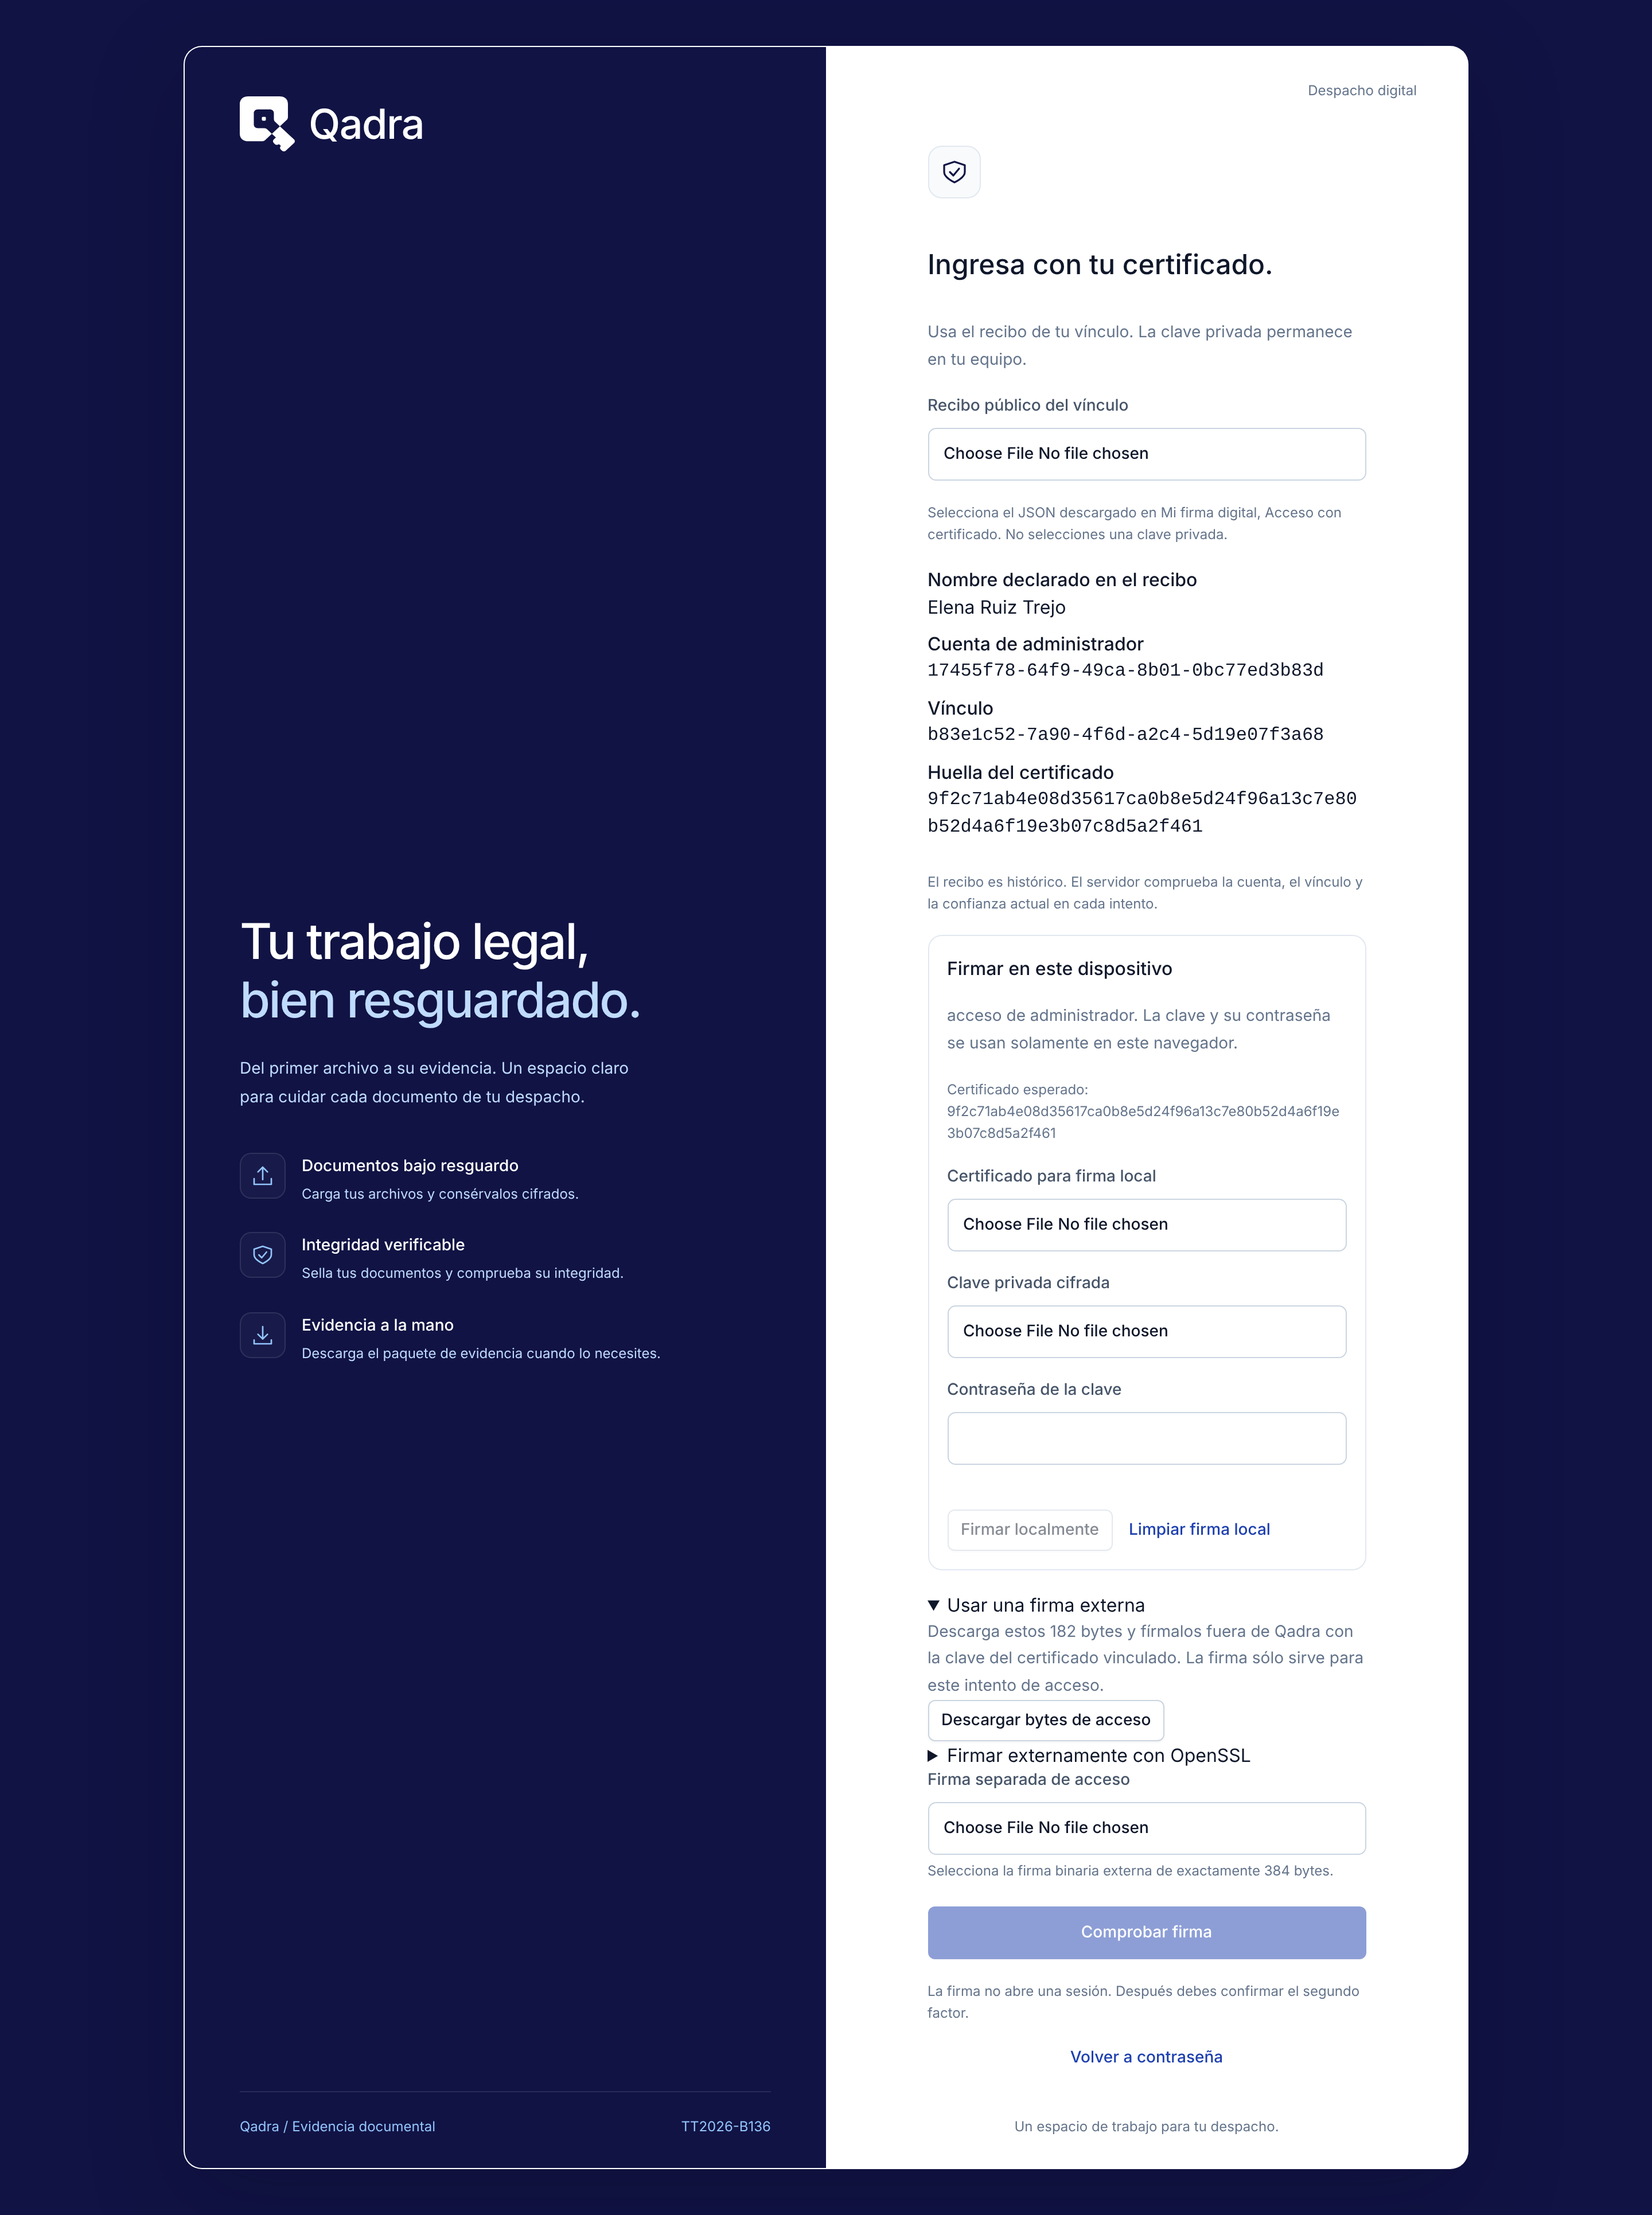
\includegraphics[width=0.9\textwidth]{capturas/A-09-ingresar-certificado.png}
  \caption{Inicio de sesión con certificado.}
  \label{fig:manual-ingresar-certificado}
\end{figure}

\resultado Se abre su espacio de trabajo como Administrador.

\begin{itemize}
  \item Su clave privada no sale de su equipo: la firma se hace en el
        navegador.
  \item Si prefiere firmar con su propia herramienta, abra
        \textbf{Usar una firma externa}, haga clic en
        \textbf{Descargar bytes de acceso}, firme el archivo
        \texttt{acceso-certificado.bin} y seleccione el resultado en
        \textbf{Firma separada de acceso}.
  \item Si tarda demasiado, aparece \enquote{El intento de acceso venció.
        Prepara otro intento y firma los nuevos bytes.} Haga clic en
        \textbf{Preparar otro intento}.
  \item Para volver al acceso normal, haga clic en
        \textbf{Volver a contraseña}.
\end{itemize}

% ---------------------------------------------------------------------
\section{Cerrar sesión y sesión terminada}\label{sec:cerrar-sesion}

\paraque Termina su sesión de forma segura cuando deja de trabajar.

\disponible Todos los roles con cuenta.

\pasos
\begin{enumerate}
  \item En la esquina superior derecha, haga clic en el círculo con sus
        iniciales (menú \textbf{Tu cuenta}).
  \item Revise su nombre, correo y rol, y haga clic en
        \textbf{Cerrar sesión}.
\end{enumerate}

\begin{figure}[H]
  \centering
  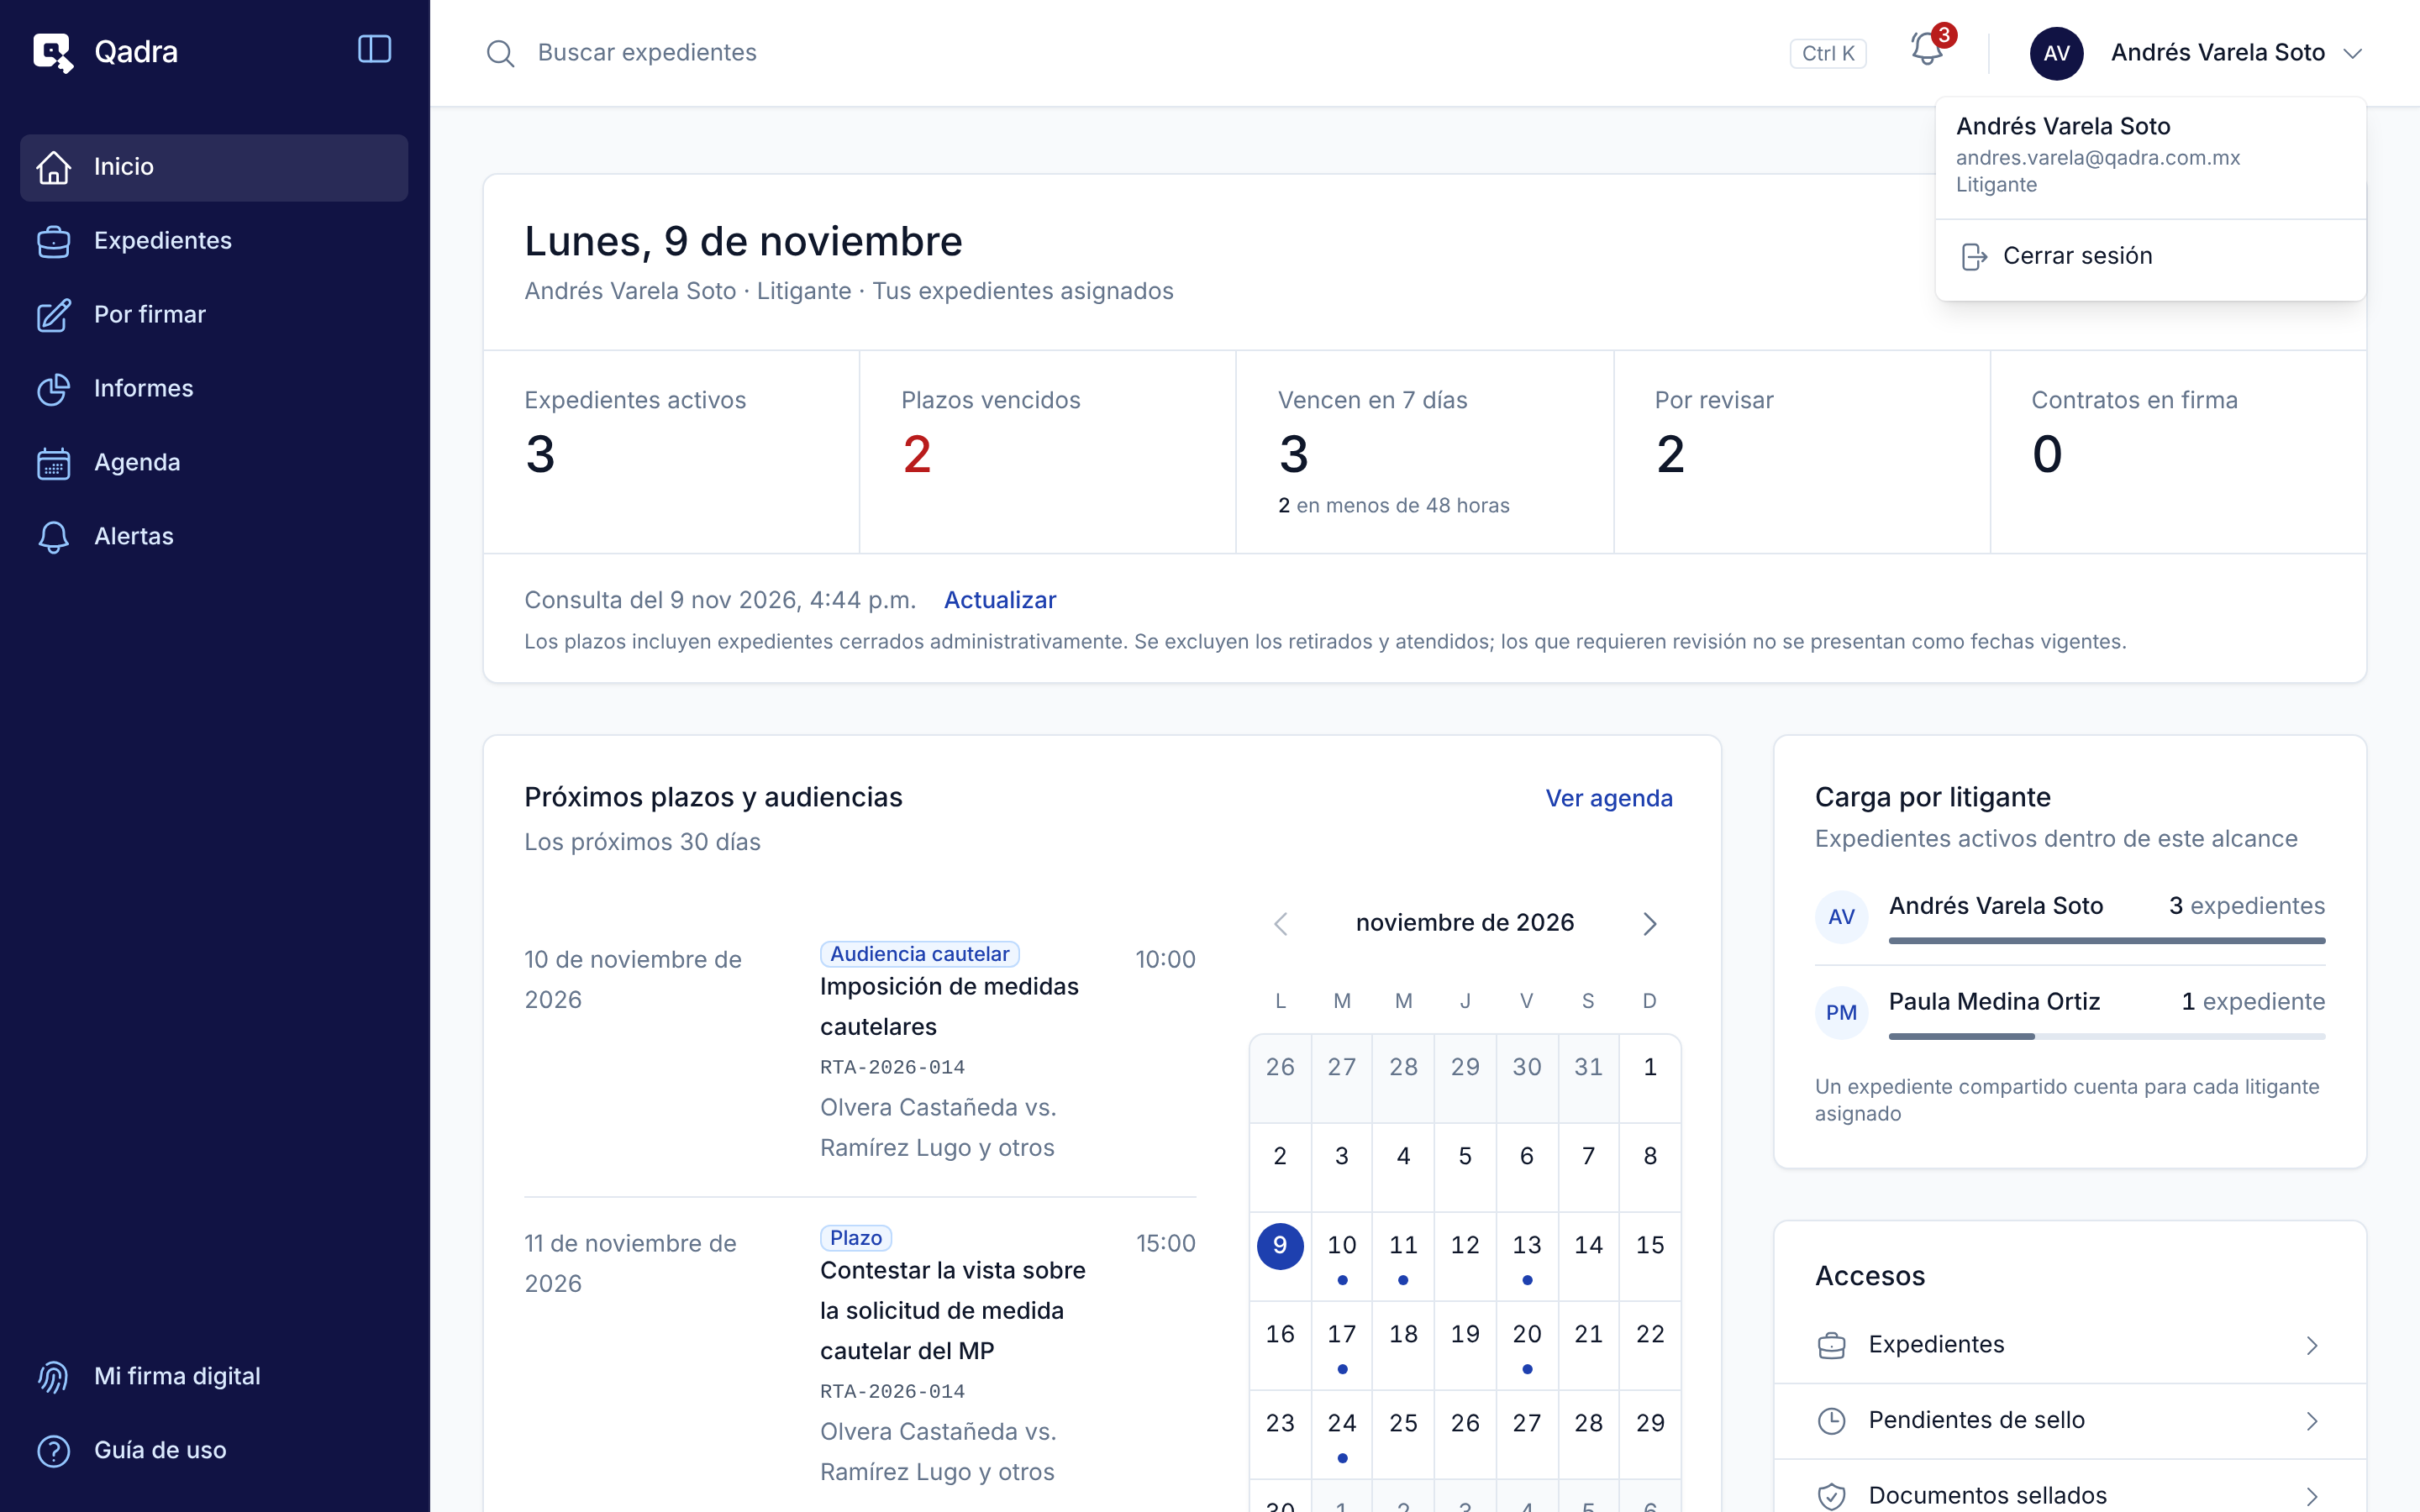
\includegraphics[width=0.9\textwidth]{capturas/A-10-menu-cuenta.png}
  \caption{Menú de la cuenta.}
  \label{fig:manual-menu-cuenta}
\end{figure}

\resultado Qadra vuelve a la pantalla de inicio de sesión.

\begin{itemize}
  \item \textbf{Sesión terminada:} si pasa mucho tiempo sin actividad, Qadra
        lo regresa al inicio de sesión con el mensaje \enquote{Tu sesión
        terminó. Vuelve a iniciar sesión.}
  \item \textbf{Al volver a la pestaña:} Qadra muestra \enquote{Comprobando
        tu sesión.} y conserva sus cambios en pantalla. Si no avanza, haga
        clic en \textbf{Comprobar de nuevo}.
  \item Si Qadra no pudo confirmar el cierre con el servidor, aparece
        \enquote{Saliste de esta pantalla. No se pudo confirmar el cierre en
        el servidor.} Cierre también la pestaña del navegador.
\end{itemize}

\chapter{Menú principal e Inicio}\label{cap:menu-inicio}

% ---------------------------------------------------------------------
\section{Menú principal}\label{sec:menu-principal}

\paraque Lleva a cada sección de Qadra. Cada rol ve solo las opciones que
puede usar.

\disponible Administrador, Litigante y Asistente legal. El menú del Cliente
se describe en la Parte B.

El menú está en el costado izquierdo de la pantalla. La \cref{tab:menu}
muestra sus opciones.

\begin{table}[H]
  \centering
  \caption{Opciones del menú principal por rol.}\label{tab:menu}
  \begin{tabularx}{\textwidth}{L{3.4cm} Y C{1.3cm} C{1.3cm} C{1.4cm}}
    \toprule
    \textbf{Opción} & \textbf{Qué abre} & \textbf{Adm.} & \textbf{Litig.} & \textbf{Asist.} \\
    \midrule
    \textbf{Inicio}            & Resumen del día y accesos rápidos. & Sí & Sí & Sí \\
    \textbf{Expedientes}       & Archivo de expedientes y cada expediente abierto. & Sí & Sí & Sí \\
    \textbf{Por firmar}        & Contratos que firma por el despacho. & Sí & Sí & No \\
    \textbf{Informes}          & Informes de expedientes en PDF y CSV. & Sí & Sí & No \\
    \textbf{Agenda}            & Audiencias y vencimientos de sus expedientes. & Sí & Sí & Sí \\
    \textbf{Alertas}           & Sus avisos personales y preferencias. & Sí & Sí & Sí \\
    \textbf{Equipo}            & Cuentas e invitaciones del despacho. & Sí & No & No \\
    \textbf{Bitácora}          & Movimientos e incidentes de integridad. & Sí & No & No \\
    \textbf{Calendarios}       & Calendarios jurisdiccionales. & Sí & No & No \\
    \textbf{Mi firma digital}  & Su clave, certificado y vínculo de firma. & Sí & Sí & No \\
    \textbf{Guía de uso}       & Ayuda breve dentro de Qadra. & Sí & Sí & Sí \\
    \bottomrule
  \end{tabularx}
\end{table}

\begin{itemize}
  \item \textbf{Equipo}, \textbf{Bitácora} y \textbf{Calendarios} aparecen
        bajo el título \textbf{Administración}.
  \item Para ganar espacio en pantallas grandes, haga clic en
        \textbf{Contraer menú}; para mostrarlo de nuevo, haga clic en
        \textbf{Expandir menú}.
  \item En el teléfono, el menú se abre con el botón \textbf{Abrir menú} de
        la barra superior.
\end{itemize}

\begin{figure}[H]
  \centering
  \capturapendiente{capturas/A-11-menu-principal.png}%
    {Pantalla completa con el menú lateral desplegado, incluida la sección Administración · Administrador}
  \caption{Menú principal del Administrador.}
  \label{fig:manual-menu-principal}
\end{figure}

% ---------------------------------------------------------------------
\section{Barra superior}\label{sec:barra-superior}

\paraque Ofrece la búsqueda rápida de expedientes, sus avisos sin leer y el
menú de su cuenta.

\disponible Administrador, Litigante y Asistente legal.

\begin{table}[H]
  \centering
  \caption{Elementos de la barra superior.}\label{tab:barra-superior}
  \begin{tabularx}{\textwidth}{L{3.6cm} Y}
    \toprule
    \textbf{Elemento} & \textbf{Cómo se usa} \\
    \midrule
    \textbf{Buscar expedientes}
      & Escriba al menos 2 caracteres del título, la referencia, el NUC o la
        carpeta judicial. Seleccione un resultado para abrirlo. También se
        activa con \texttt{Ctrl}+\texttt{K}. \\
    Campana de avisos
      & Muestra el panel \textbf{Avisos sin leer}. Haga clic en
        \textbf{Abrir la bandeja de alertas} para ver todos en
        \textbf{Alertas}. \\
    Círculo con sus iniciales (\textbf{Tu cuenta})
      & Muestra su nombre, correo y rol, y el botón
        \textbf{Cerrar sesión} (\cref{sec:cerrar-sesion}). \\
    \bottomrule
  \end{tabularx}
\end{table}

\nota{La búsqueda rápida cubre los primeros 300 expedientes. Si no encuentra
uno, haga clic en \textbf{Ir al archivo de expedientes} y use los filtros
(\cref{sec:buscar-expediente}).}

% ---------------------------------------------------------------------
\section{Inicio}\label{sec:inicio}

\paraque Muestra su situación del día y lo lleva rápido a sus pendientes.

\disponible Administrador, Litigante y Asistente legal. El contenido cambia
según el rol.

\subsection*{Inicio del Administrador y del Litigante}

El Administrador ve los datos de \textbf{Todo el despacho}; el Litigante, los
de \textbf{Tus expedientes asignados}.

\begin{itemize}
  \item \textbf{Indicadores:} \textbf{Expedientes activos},
        \textbf{Plazos vencidos}, \textbf{Vencen en 7 días},
        \textbf{Por revisar} y \textbf{Contratos en firma}. Haga clic en
        \textbf{Actualizar} para recalcularlos.
  \item \textbf{Próximos plazos y audiencias:} actividades de los próximos
        30 días. Haga clic en una actividad o en \textbf{Ver agenda} para
        abrir la \textbf{Agenda}.
  \item \textbf{Carga por litigante:} cuántos expedientes activos tiene
        asignados cada litigante.
\end{itemize}

\begin{figure}[H]
  \centering
  \capturapendiente{capturas/A-12-inicio-tablero.png}%
    {Inicio con indicadores, próximos plazos y audiencias y carga por litigante · Litigante}
  \caption{Inicio del Administrador y del Litigante.}
  \label{fig:manual-inicio-tablero}
\end{figure}

\subsection*{Inicio del Asistente legal}

\begin{itemize}
  \item \textbf{Tu expediente actual:} haga clic en
        \textbf{Abrir expediente} para continuar con el último expediente,
        o en \textbf{Seleccionar expediente} si aún no eligió uno.
  \item \textbf{Accesos:} atajos a \textbf{Expedientes},
        \textbf{Pendientes de sello}, \textbf{Documentos sellados} y
        \textbf{Mis alertas}.
  \item \textbf{Tu siguiente paso:} recuerda el recorrido de un documento:
        \textbf{Carga}, \textbf{Sella} y \textbf{Verifica y descarga}.
\end{itemize}

\begin{figure}[H]
  \centering
  \capturapendiente{capturas/A-13-inicio-asistente.png}%
    {Inicio con Tu expediente actual, Accesos y Tu siguiente paso · Asistente legal}
  \caption{Inicio del Asistente legal.}
  \label{fig:manual-inicio-asistente}
\end{figure}

\resultado Desde \textbf{Inicio} llega en un clic a sus expedientes, su
agenda o sus documentos pendientes.

\nota{La opción \textbf{Guía de uso} del menú resume, dentro de Qadra, las
tareas más comunes y responde preguntas frecuentes.}

\chapter{Expedientes}\label{cap:expedientes}

% ---------------------------------------------------------------------
\section{Buscar y abrir un expediente}\label{sec:buscar-expediente}

\paraque Localiza un expediente del archivo y lo abre para trabajar en él.

\disponible Administrador (todos los expedientes), Litigante y Asistente
legal (solo los expedientes que tienen asignados).

\pasos
\begin{enumerate}
  \item En el menú, haga clic en \textbf{Expedientes}. Aparece el
        \textbf{Archivo de expedientes}.
  \item Para filtrar, use uno o varios campos:
        \begin{itemize}
          \item \textbf{Buscar por título}: basta una parte del título.
          \item \textbf{Estado administrativo}: \textbf{Activos},
                \textbf{Cerrados} o \textbf{Todos}.
          \item \textbf{Ficha penal}: \textbf{Todas}, \textbf{Completas} o
                \textbf{Pendientes}.
          \item \textbf{Más filtros}: al hacer clic se muestran
                \textbf{NUC exacto} y \textbf{Carpeta judicial exacta}, que
                deben coincidir por completo, incluidas mayúsculas y acentos.
                El número entre paréntesis indica cuántos están en uso.
        \end{itemize}
  \item Haga clic en \textbf{Buscar expedientes}.
  \item Haga clic en la tarjeta del expediente que desea abrir. Use
        \textbf{Anterior} y \textbf{Siguiente} para recorrer las páginas.
\end{enumerate}

\begin{figure}[H]
  \centering
  \capturapendiente{capturas/A-14-archivo-expedientes.png}%
    {Archivo de expedientes con filtros y tarjetas (Activo, Ficha completa) · Litigante}
  \caption{Archivo de expedientes.}
  \label{fig:manual-archivo-expedientes}
\end{figure}

\resultado Se abre el \textbf{Resumen} del expediente
(\cref{sec:resumen-expediente}).

\begin{itemize}
  \item Cada tarjeta indica si el expediente está \textbf{Activo} o
        \textbf{Cerrado administrativamente}, y si su ficha está
        \textbf{Ficha completa} o \textbf{Ficha pendiente}.
  \item Si no aparece ningún expediente, el Litigante o el Asistente legal
        verá \enquote{El administrador puede asignarte un expediente para
        comenzar.}
\end{itemize}

% ---------------------------------------------------------------------
\section{Crear un expediente penal}\label{sec:crear-expediente}

\paraque Registra un expediente nuevo con su ficha penal completa.

\disponible Administrador y Litigante. El Litigante que lo crea queda
asignado al expediente.

\pasos
\begin{enumerate}
  \item En \textbf{Expedientes}, haga clic en
        \textbf{Nuevo expediente penal}.
  \item Ingrese el \textbf{Título del expediente} y la
        \textbf{Referencia interna} del despacho.
  \item En \textbf{Identificadores registrados}, ingrese:
        \textbf{NUC}, \textbf{Autoridad emisora del NUC},
        \textbf{Carpeta judicial} y \textbf{Órgano emisor de la carpeta}.
  \item Si lo desea, complete \textbf{Información general (opcional)} e
        \textbf{Identificadores complementarios (opcional)}.
  \item En \textbf{Delitos registrados}, escriba un delito en
        \textbf{Nueva descripción de delito} y haga clic en
        \textbf{Agregar descripción}. Repita para cada delito (de 1 a 8).
  \item Revise el aviso \enquote{Se creará un expediente activo con etapa
        registrada Investigación.} y haga clic en
        \textbf{Crear expediente penal}.
\end{enumerate}

\begin{figure}[H]
  \centering
  \capturapendiente{capturas/A-15-nuevo-expediente.png}%
    {Formulario Nuevo expediente penal con identificadores y delitos registrados · Litigante}
  \caption{Registro de un expediente penal.}
  \label{fig:manual-nuevo-expediente}
\end{figure}

\resultado El expediente aparece en el archivo como \textbf{Activo}, con
\textbf{Ficha completa} y la etapa inicial \textbf{Investigación}.

\begin{itemize}
  \item Si el NUC o la carpeta ya existen, aparece \enquote{El NUC o la
        carpeta judicial ya están registrados. Revisa ambos
        identificadores.}
  \item Qadra registra los datos tal como se escriben; no los verifica ante
        las instituciones.
  \item Para quitar un delito de la lista, haga clic en \textbf{Quitar}.
\end{itemize}

% ---------------------------------------------------------------------
\section{Consultar el Resumen del expediente}\label{sec:resumen-expediente}

\paraque Muestra la ficha penal, el estado administrativo, la etapa inicial
y el historial de cambios del expediente.

\disponible Administrador, Litigante y Asistente legal.

Al abrir un expediente, la parte superior muestra su título, su referencia y
el botón \textbf{Cambiar expediente}. Debajo aparecen las pestañas de la
\cref{tab:pestanas}.

\begin{table}[H]
  \centering
  \caption{Pestañas de un expediente.}\label{tab:pestanas}
  \begin{tabularx}{\textwidth}{L{3.4cm} Y}
    \toprule
    \textbf{Pestaña} & \textbf{Contenido} \\
    \midrule
    \textbf{Resumen}            & Ficha penal, estado y etapa inicial. \\
    \textbf{Documentos}         & Archivos del expediente, sello y evidencia. \\
    \textbf{Participantes}      & Personas que intervienen en el expediente. \\
    \textbf{Etapas}             & Etapa procesal actual y sus cambios. \\
    \textbf{Audiencias}         & Audiencias, sus resultados y audiencias cautelares. \\
    \textbf{Medidas cautelares} & Decisiones y registros de medidas. \\
    \textbf{Resoluciones}       & Resoluciones y sus notificaciones. \\
    \textbf{Recursos}           & Revocaciones y apelaciones. \\
    \textbf{Plazos}             & Cómputo y atención de plazos. \\
    \textbf{Contratos}          & Contratos firmados con el Cliente. \\
    \textbf{Asignaciones}       & Cuentas con acceso al expediente (solo Administrador). \\
    \bottomrule
  \end{tabularx}
\end{table}

\pasos
\begin{enumerate}
  \item Abra el expediente (\cref{sec:buscar-expediente}). Se muestra la
        pestaña \textbf{Resumen}.
  \item Revise la ficha: \textbf{Ficha penal completa} o
        \textbf{Ficha penal pendiente}, sus datos y el estado
        \textbf{Activo} o \textbf{Cerrado administrativamente}.
  \item Para ver quién cambió la ficha y cuándo, haga clic en
        \textbf{Ver historial administrativo}.
  \item Para ir a la etapa procesal, haga clic en
        \textbf{Consultar etapas}.
\end{enumerate}

\begin{figure}[H]
  \centering
  \capturapendiente{capturas/A-16-resumen-expediente.png}%
    {Pestaña Resumen con ficha penal completa, estado y Registro inicial de etapa · Litigante}
  \caption{Resumen del expediente.}
  \label{fig:manual-resumen-expediente}
\end{figure}

\resultado Conoce el estado actual del expediente antes de trabajar en sus
pestañas. Haga clic en \textbf{Actualizar resumen} si otra persona pudo
modificarlo.

\nota{En pantallas pequeñas, las pestañas se muestran como una lista
desplegable.}

% ---------------------------------------------------------------------
\section{Editar o completar la ficha penal}\label{sec:editar-ficha}

\paraque Corrige los datos del expediente o completa la ficha de un
expediente que quedó pendiente.

\disponible Administrador y Litigante asignado. El expediente debe estar
activo.

\pasos
\begin{enumerate}
  \item En el \textbf{Resumen}, haga clic en el botón que corresponda:
        \begin{itemize}
          \item \textbf{Editar ficha penal}, si la ficha está completa.
          \item \textbf{Editar datos básicos} o
                \textbf{Completar ficha penal}, si la ficha está pendiente.
        \end{itemize}
  \item Modifique los campos necesarios (los mismos de la
        \cref{sec:crear-expediente}).
  \item Haga clic en \textbf{Guardar ficha penal} o
        \textbf{Guardar datos básicos}.
\end{enumerate}

\resultado El Resumen muestra los datos nuevos y el historial administrativo
registra la revisión con su autor y fecha.

\begin{itemize}
  \item \textbf{Si otra persona cambió la ficha al mismo tiempo}, aparece
        \enquote{Los datos del expediente cambiaron. Consulta los valores
        actuales.} Haga clic en \textbf{Consultar datos actuales}, compare
        los \textbf{Valores actuales guardados} con su formulario, marque
        \textbf{He comparado los valores actuales y decido guardar mis
        cambios} y haga clic en \textbf{Guardar mis cambios}.
  \item Completar una ficha pendiente no crea una etapa procesal; regístrela
        después en la pestaña \textbf{Etapas}.
\end{itemize}

% ---------------------------------------------------------------------
\section{Cerrar o reactivar un expediente}\label{sec:cerrar-expediente}

\paraque Suspende los cambios de un expediente concluido, o los permite de
nuevo.

\disponible Administrador y Litigante asignado.

\importante{Un expediente cerrado conserva la consulta, el historial, la
verificación y la descarga de evidencia, pero no admite cambios en la ficha,
documentos, participantes, etapas, audiencias ni plazos hasta que se
reactive. Cerrar no cambia la etapa procesal registrada.}

\pasos
\begin{enumerate}
  \item En el \textbf{Resumen}, haga clic en
        \textbf{Cerrar administrativamente} (o en
        \textbf{Reactivar expediente} si ya está cerrado).
  \item Lea el aviso de la ventana y revise los datos del expediente.
  \item Haga clic en \textbf{Confirmar cierre administrativo} (o en
        \textbf{Confirmar reactivación}).
\end{enumerate}

\begin{figure}[H]
  \centering
  \capturapendiente{capturas/A-17-cerrar-expediente.png}%
    {Ventana Cerrar administrativamente con su aviso y el botón de confirmación · Litigante}
  \caption{Cierre administrativo de un expediente.}
  \label{fig:manual-cerrar-expediente}
\end{figure}

\resultado El expediente muestra \textbf{Cerrado administrativamente} y, en
todas sus pestañas, el aviso \enquote{Expediente cerrado administrativamente.
Puedes consultar, verificar y exportar; las modificaciones están
suspendidas.}

\nota{Si estaba llenando un formulario cuando otra persona cerró el
expediente, Qadra conserva su formulario. Haga clic en
\textbf{Consultar estado del expediente} y, si corresponde, reactive el
expediente antes de guardar. Reactivar no reenvía sus cambios
automáticamente.}

\chapter{Documentos}\label{cap:documentos}

Todos los documentos viven dentro de un expediente. Antes de cualquier tarea
de este capítulo, abra el expediente (\cref{sec:buscar-expediente}) y haga
clic en la pestaña \textbf{Documentos}.

\begin{table}[H]
  \centering
  \caption{Qué puede hacer cada rol con los documentos.}\label{tab:permisos-documentos}
  \begin{tabularx}{\textwidth}{Y C{1.4cm} C{1.4cm} C{1.4cm}}
    \toprule
    \textbf{Acción} & \textbf{Adm.} & \textbf{Litig.} & \textbf{Asist.} \\
    \midrule
    Consultar, subir, clasificar y agregar versiones & Sí & Sí & Sí \\
    Descargar el archivo, verificar y descargar evidencia & Sí & Sí & Sí \\
    Sellar documento & Sí & Sí & No \\
    Crear contrato con el Cliente & Sí & Sí & No \\
    Firmar personalmente & No & Sí & No \\
    \bottomrule
  \end{tabularx}
\end{table}

El Litigante y el Asistente legal solo ven los documentos de sus expedientes
asignados.

% ---------------------------------------------------------------------
\section{Consultar los documentos del expediente}\label{sec:consultar-documentos}

\paraque Localiza un documento del expediente y muestra en qué estado se
encuentra.

\disponible Administrador, Litigante y Asistente legal.

\pasos
\begin{enumerate}
  \item En la pestaña \textbf{Documentos}, revise el \textbf{Archivo documental}.
  \item Para buscar, escriba parte del nombre en \textbf{Buscar por nombre...}
        y haga clic en \textbf{Buscar}.
  \item Para filtrar por estado, elija \textbf{Todos los estados},
        \textbf{Pendientes de sello} o \textbf{Sellados}.
  \item Para filtrar por clasificación, abra \textbf{Filtros de clasificación},
        llene \textbf{Tipo exacto}, \textbf{Clasificación exacta} o
        \textbf{Etiqueta exacta} y haga clic en \textbf{Aplicar filtros}.
  \item Haga clic en \textbf{Abrir} junto al documento.
\end{enumerate}

\begin{figure}[H]
  \centering
  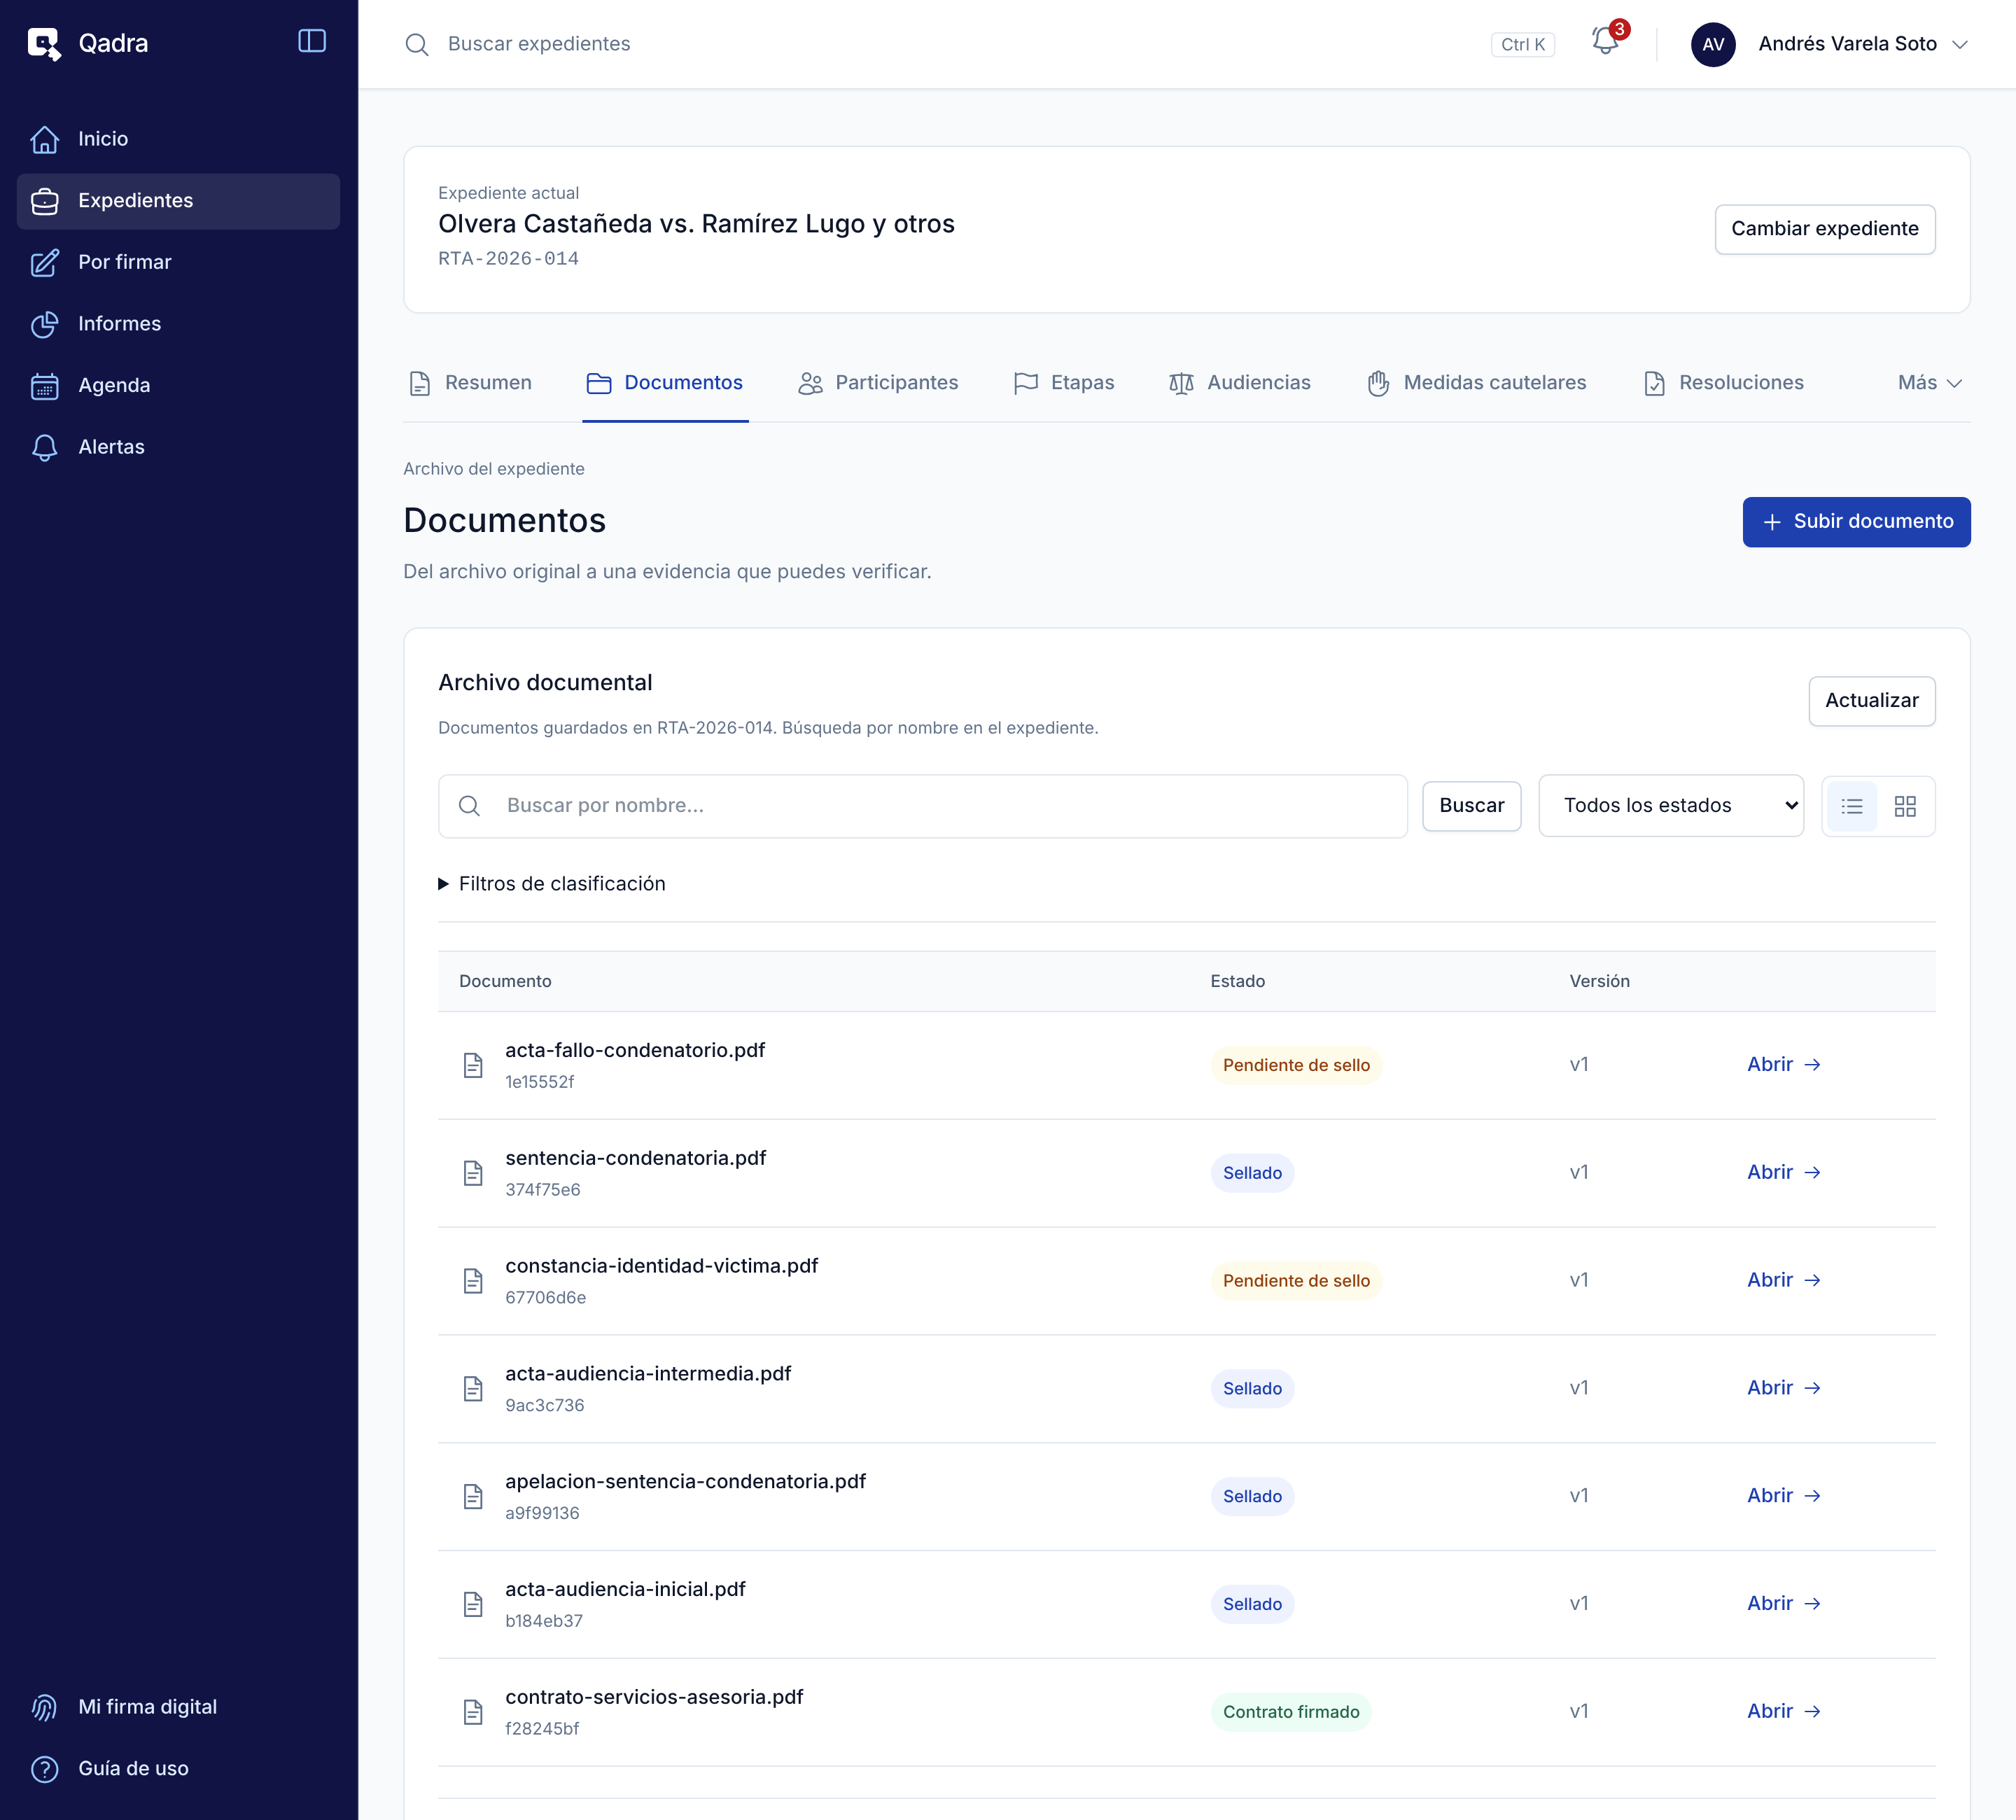
\includegraphics[width=0.9\textwidth]{capturas/A-18-archivo-documental.png}
  \caption{Archivo documental del expediente.}
  \label{fig:manual-archivo-documental}
\end{figure}

\resultado Se abre la \textbf{Ficha documental} del documento
(\cref{sec:ficha-documental}).

\begin{table}[H]
  \centering
  \caption{Estados de un documento en la lista.}\label{tab:estados-documento}
  \begin{tabularx}{\textwidth}{L{3.6cm} Y}
    \toprule
    \textbf{Estado} & \textbf{Qué significa} \\
    \midrule
    \textbf{Pendiente de sello} & El archivo está guardado, pero aún no tiene sello. \\
    \textbf{Sellado}            & Tiene firma y sello de tiempo; ya puede verificarse. \\
    \textbf{Verificado}         & La última verificación pasó todas las comprobaciones. \\
    \textbf{Revisar evidencia}  & La última verificación encontró un problema
                                  (\cref{sec:verificar-documento}). \\
    \textbf{En contrato}        & La versión está en firma con el Cliente. \\
    \textbf{Contrato firmado}   & El Cliente y el despacho firmaron la versión. \\
    \bottomrule
  \end{tabularx}
\end{table}

\nota{Los filtros de clasificación buscan el valor completo y distinguen
mayúsculas y acentos. Para quitarlos, haga clic en \textbf{Limpiar filtros}.}

% ---------------------------------------------------------------------
\section{Subir un documento}\label{sec:subir-documento}

\paraque Agrega un archivo al expediente y lo guarda cifrado como su
versión 1.

\disponible Administrador, Litigante y Asistente legal. El expediente debe
estar activo.

\pasos
\begin{enumerate}
  \item En la pestaña \textbf{Documentos}, haga clic en
        \textbf{Subir documento}.
  \item Arrastre su archivo a la zona \textbf{Arrastra tu archivo aquí}, o
        haga clic en ella para seleccionarlo desde su equipo.
  \item Revise el \textbf{Nombre del documento} que Qadra sugiere. Puede
        cambiarlo usando solo letras sin acentos, números, puntos, guiones o
        guiones bajos (hasta 124 caracteres).
  \item Si lo desea, indique el \textbf{Tipo de documento (opcional)}, la
        \textbf{Clasificación (opcional)} y sus etiquetas
        (\cref{sec:clasificar-documento}).
  \item Haga clic en \textbf{Cargar documento}.
\end{enumerate}

\begin{figure}[H]
  \centering
  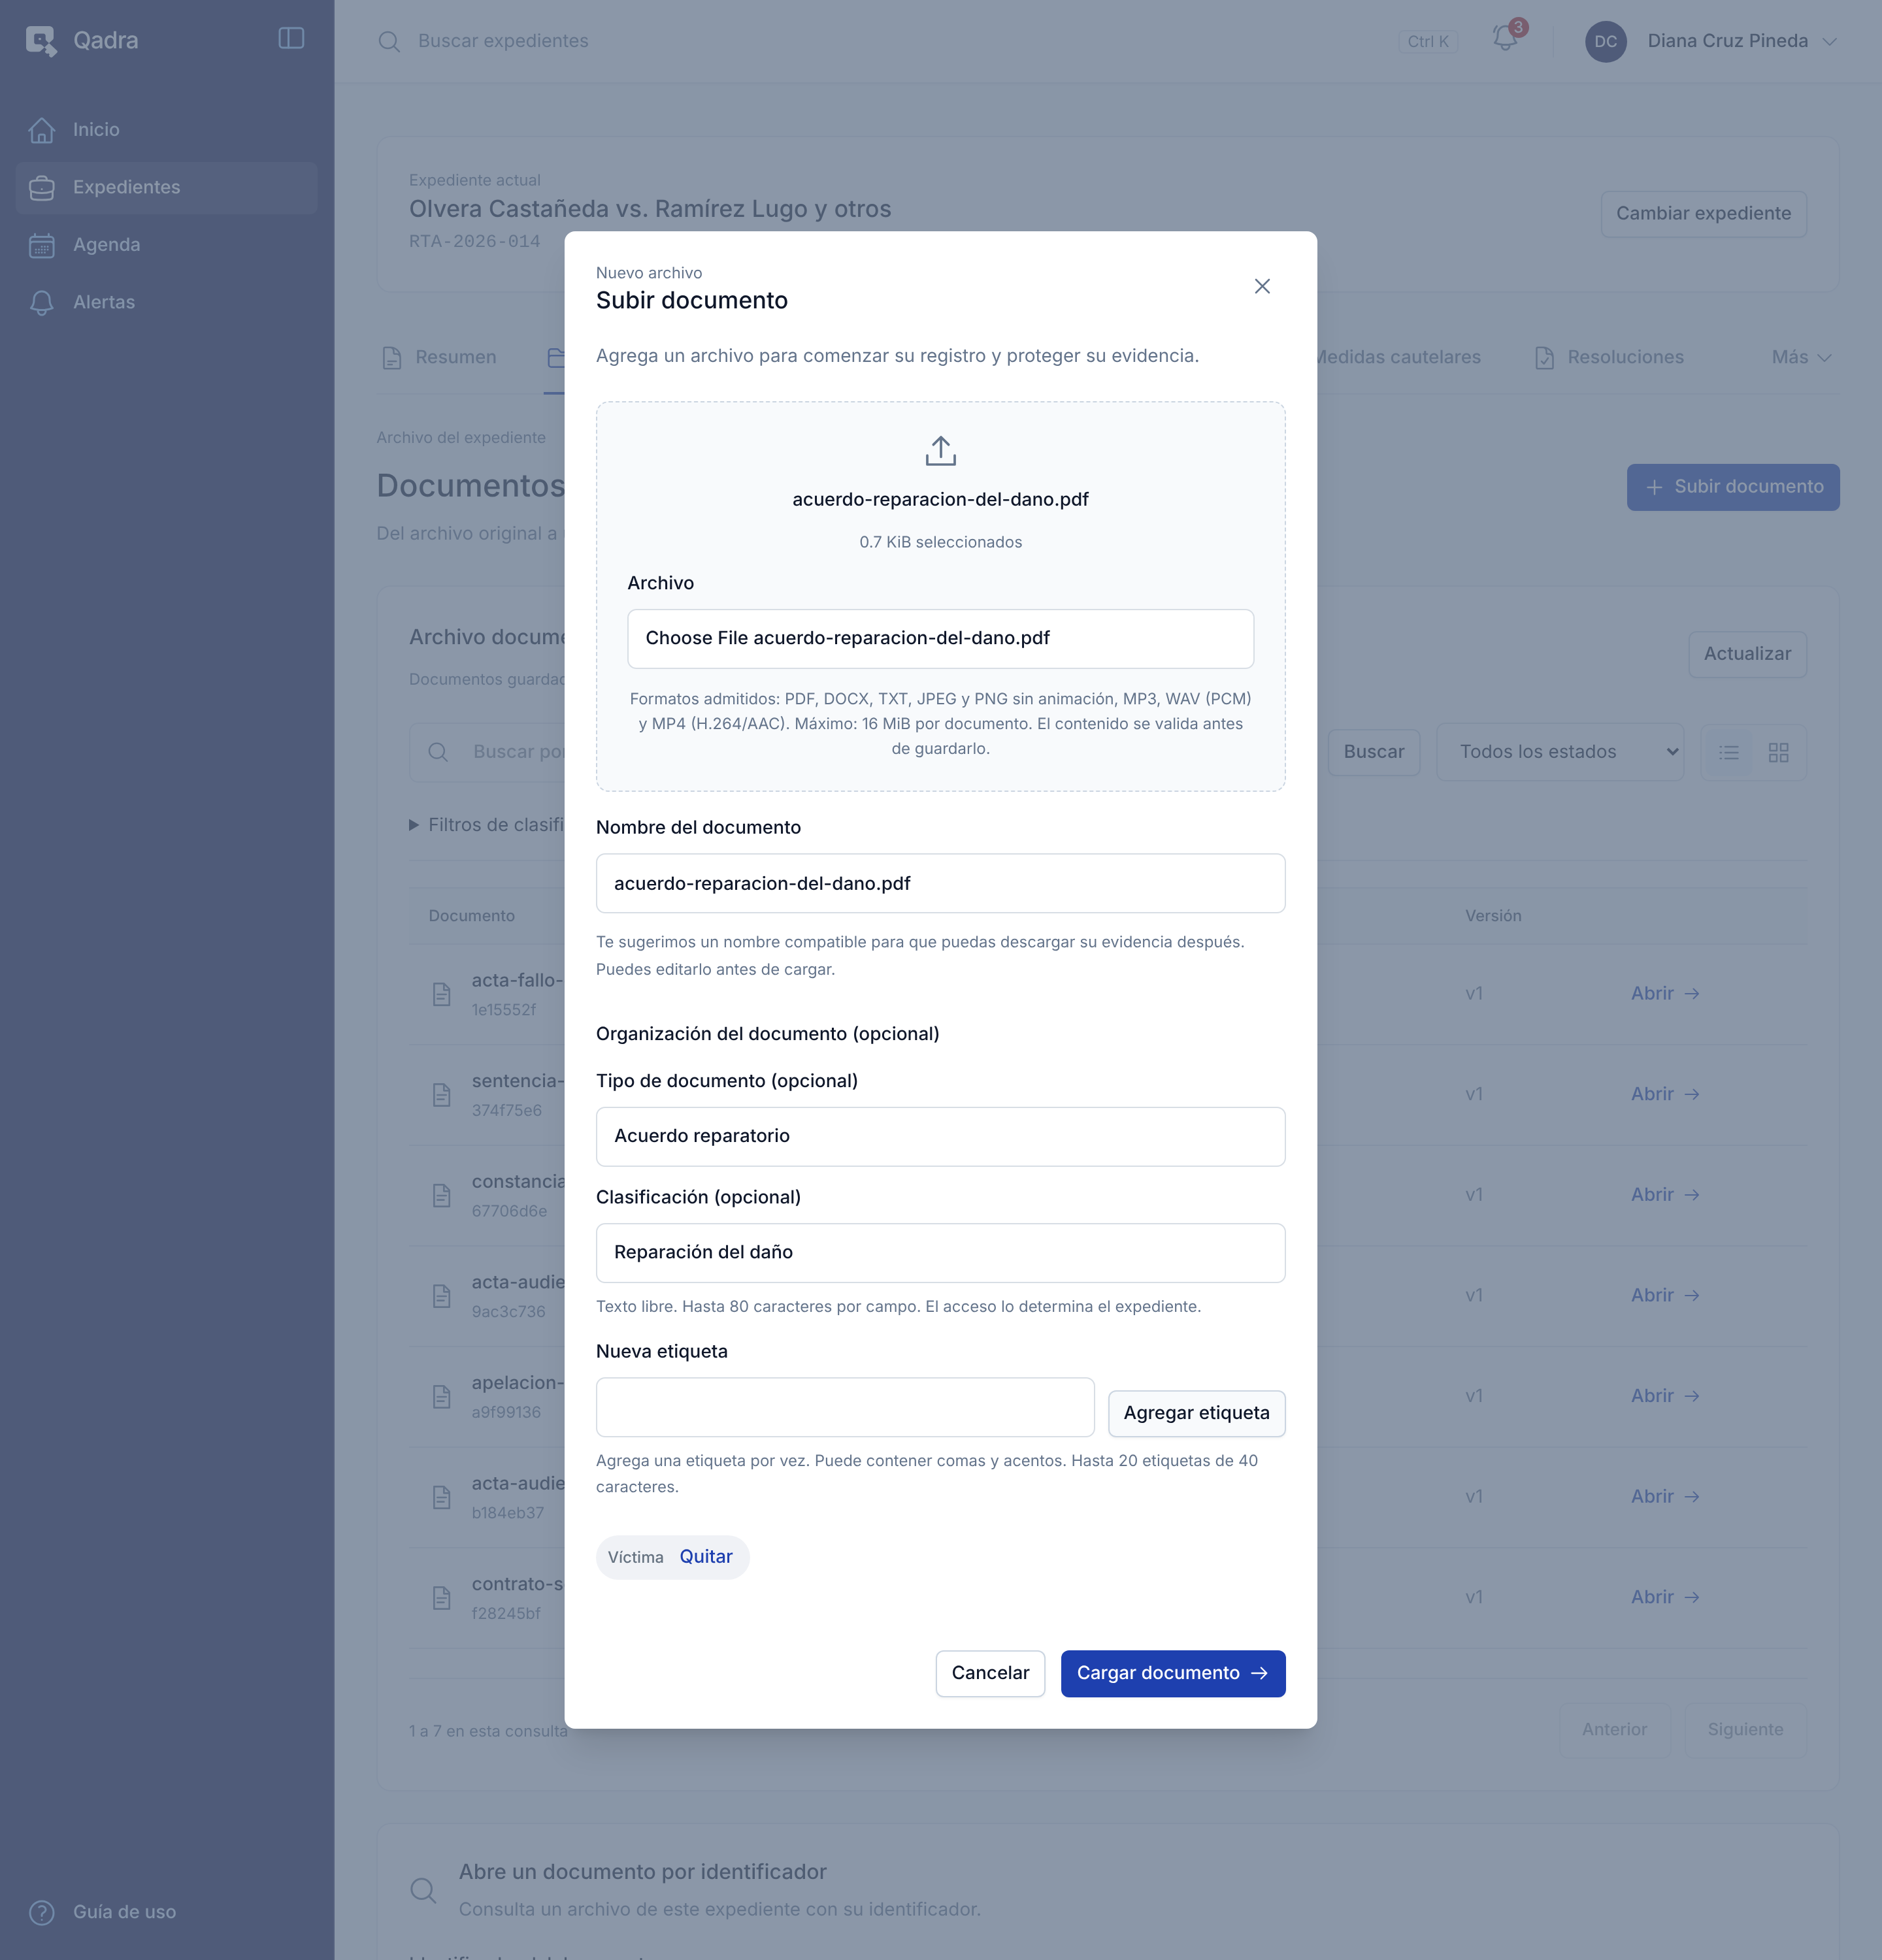
\includegraphics[width=0.9\textwidth]{capturas/A-19-subir-documento.png}
  \caption{Carga de un documento.}
  \label{fig:manual-subir-documento}
\end{figure}

\resultado El documento aparece en el archivo como
\textbf{Pendiente de sello}, en su versión 1.

\begin{table}[H]
  \centering
  \caption{Archivos admitidos.}\label{tab:formatos}
  \begin{tabularx}{\textwidth}{L{3.6cm} Y}
    \toprule
    \textbf{Concepto} & \textbf{Regla} \\
    \midrule
    Formatos & PDF, DOCX, TXT, JPEG y PNG sin animación, MP3, WAV (PCM) y
               MP4 (H.264/AAC). \\
    Tamaño máximo & 16 MiB por documento. \\
    Validación & Qadra revisa el contenido antes de guardarlo. Un archivo
                 dañado o de otro formato se rechaza. \\
    \bottomrule
  \end{tabularx}
\end{table}

\begin{itemize}
  \item Si el archivo es demasiado grande: \enquote{El archivo supera el
        límite de 16 MiB.}
  \item Si el formato no se admite: \enquote{El formato del archivo no está
        admitido. Elige un archivo de un formato compatible.}
  \item Si la carga se interrumpe, aparece \enquote{No se pudo confirmar la
        carga anterior.} Haga clic en \textbf{Consultar documentos actuales}
        antes de cargarlo otra vez, para no duplicarlo.
\end{itemize}

% ---------------------------------------------------------------------
\section{Ficha de un documento}\label{sec:ficha-documental}

\paraque Reúne el estado, las acciones, la clasificación y las versiones de
un documento.

\disponible Administrador, Litigante y Asistente legal.

La \textbf{Ficha documental} tiene, de arriba hacia abajo:
\begin{itemize}
  \item \textbf{Acciones:} \textbf{Descargar archivo},
        \textbf{Sellar documento}, \textbf{Verificar integridad},
        \textbf{Descargar evidencia} y, según el rol, \textbf{Crear contrato}
        o \textbf{Firmar personalmente}.
  \item \textbf{Pestañas:} \textbf{Resumen} (el recorrido del documento),
        \textbf{Verificación} (el resultado de la última verificación) y
        \textbf{Evidencia} (el paquete ZIP).
  \item \textbf{Clasificación actual del documento}
        (\cref{sec:clasificar-documento}).
  \item \textbf{Versiones de contenido} (\cref{sec:agregar-version}).
\end{itemize}

\begin{figure}[H]
  \centering
  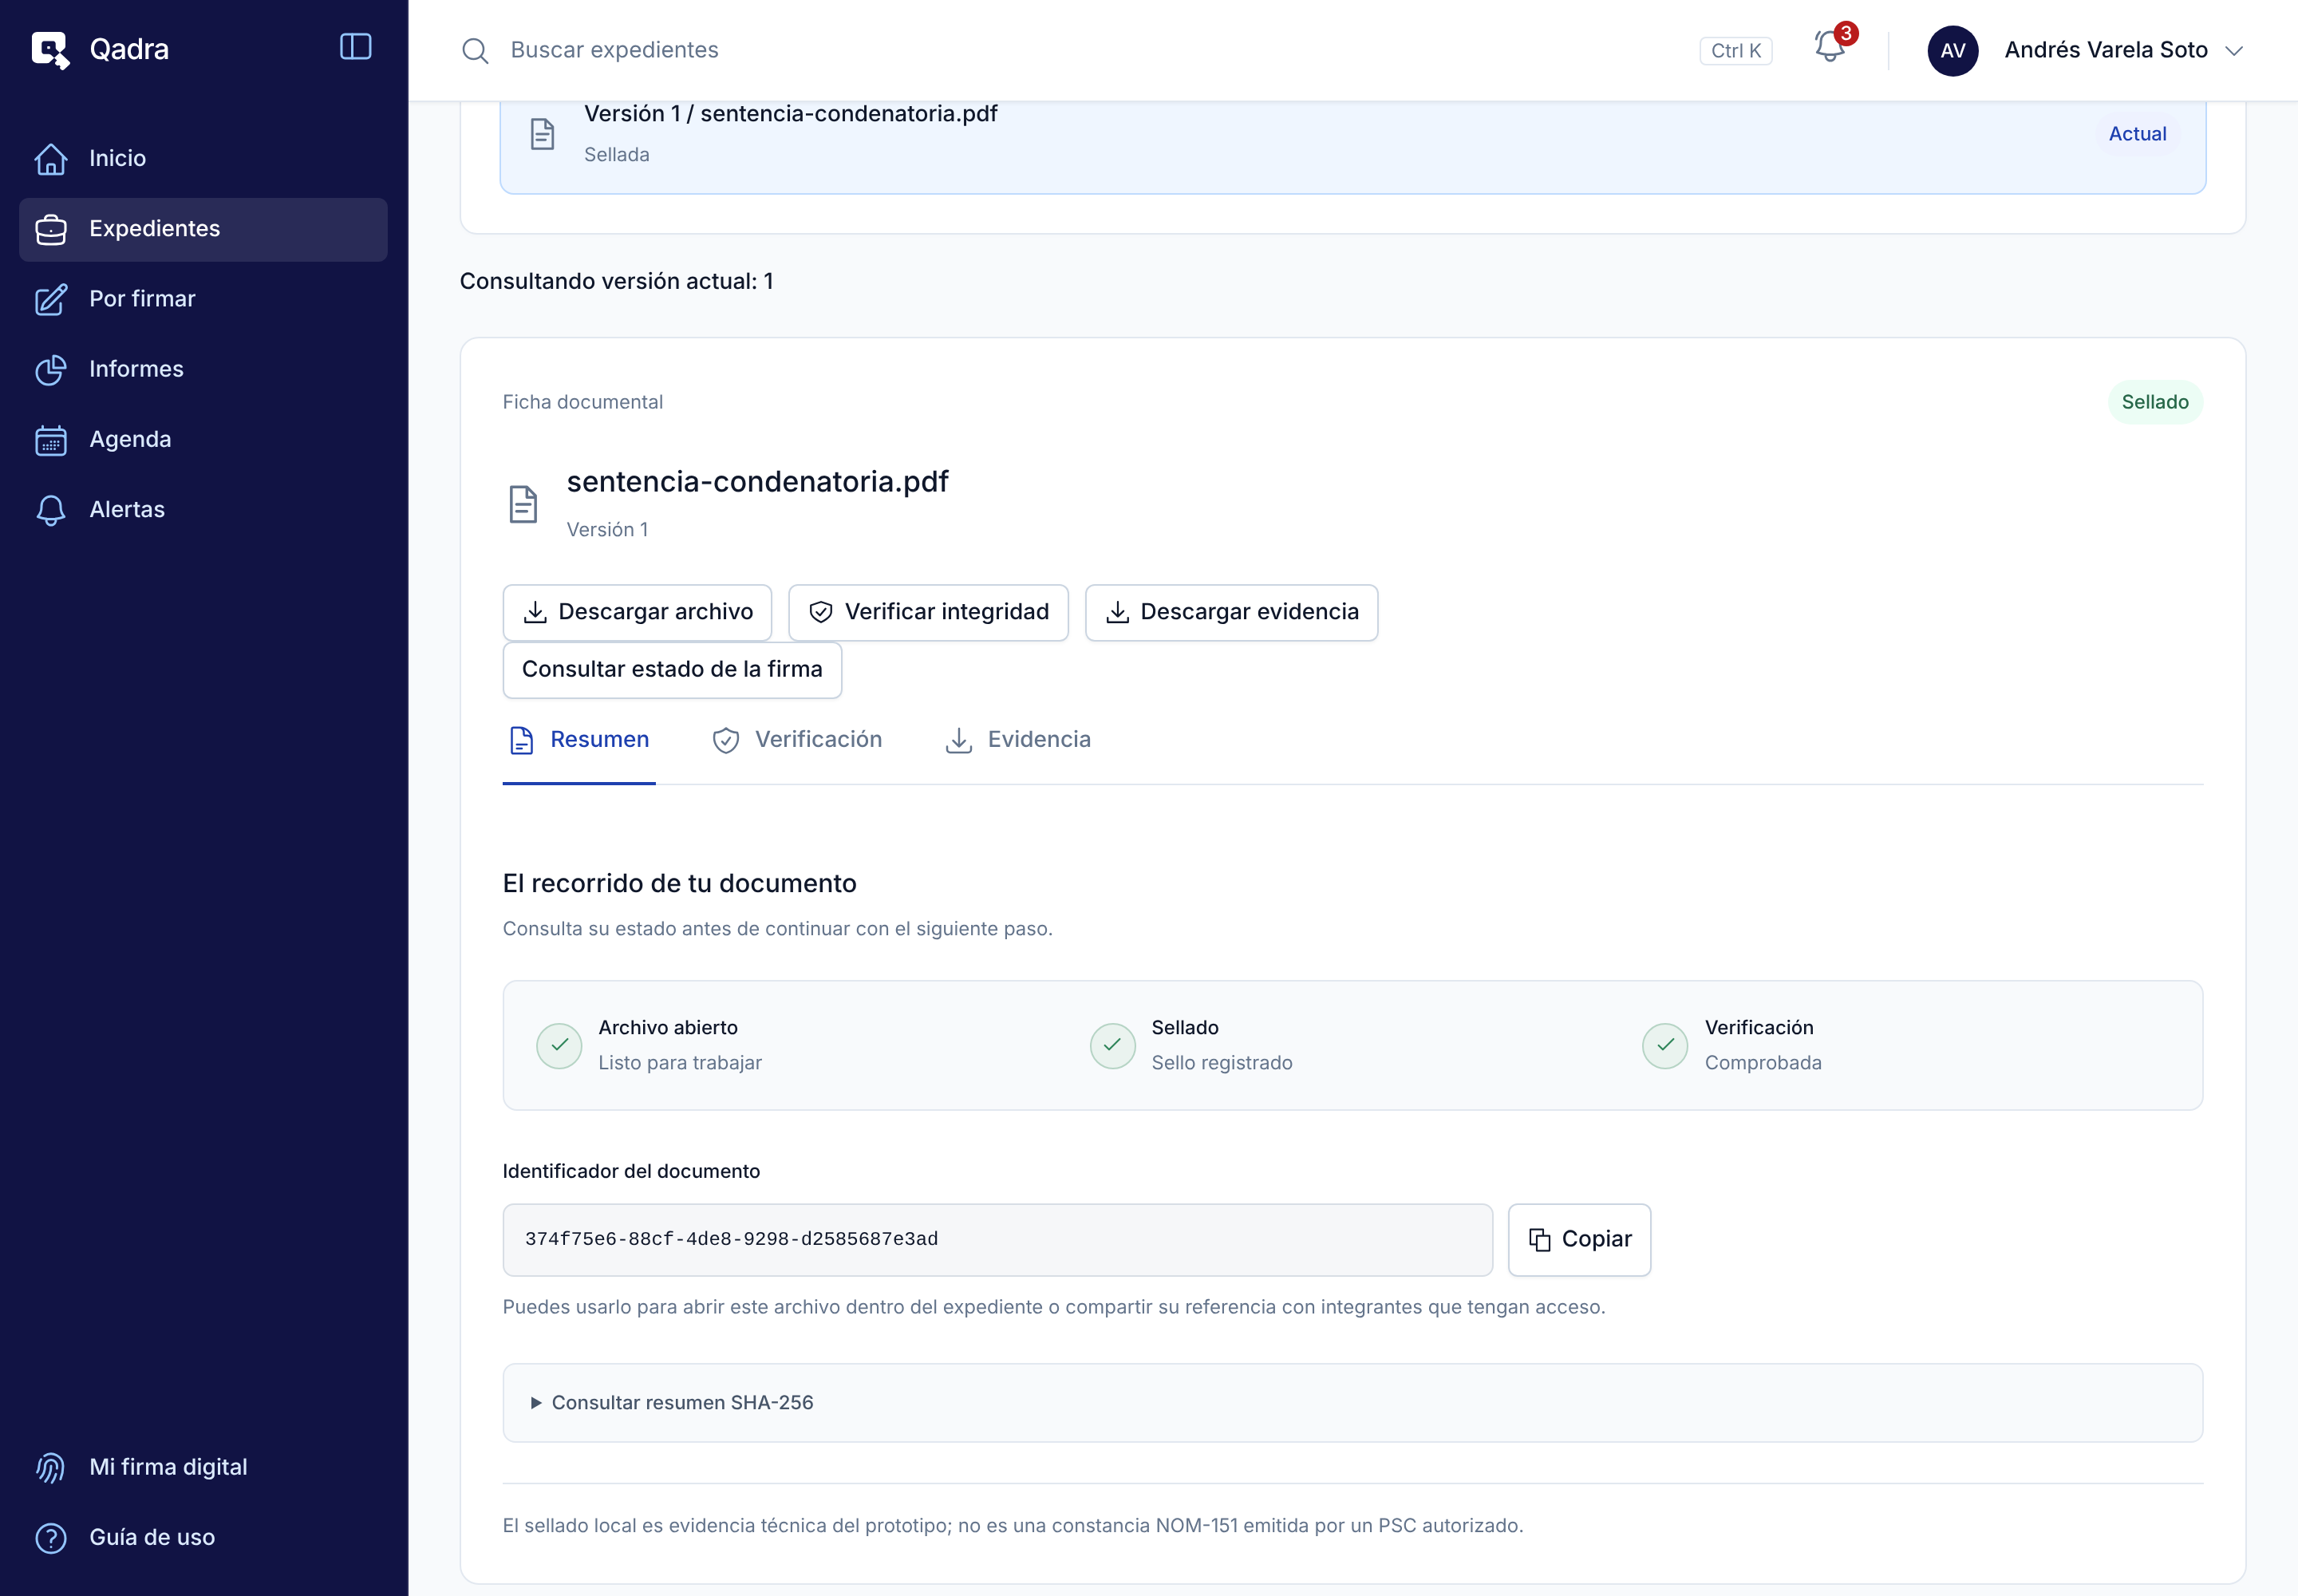
\includegraphics[width=0.9\textwidth]{capturas/A-20-ficha-documental.png}
  \caption{Ficha documental.}
  \label{fig:manual-ficha-documental}
\end{figure}

\begin{itemize}
  \item \textbf{Descargar archivo} entrega el archivo original de la versión
        elegida, después de comprobar que no cambió.
  \item En la pestaña \textbf{Resumen}, el botón \textbf{Copiar} copia el
        \textbf{Identificador del documento} para compartirlo con integrantes
        que tengan acceso.
\end{itemize}

% ---------------------------------------------------------------------
\section{Clasificar y etiquetar un documento}\label{sec:clasificar-documento}

\paraque Organiza el documento por tipo, clasificación y etiquetas para
encontrarlo después.

\disponible Administrador, Litigante y Asistente legal.

\pasos
\begin{enumerate}
  \item En la ficha del documento, busque
        \textbf{Clasificación actual del documento} y haga clic en
        \textbf{Editar clasificación}.
  \item Escriba el \textbf{Tipo de documento (opcional)} y la
        \textbf{Clasificación (opcional)}, de hasta 80 caracteres cada uno.
  \item Escriba una etiqueta en \textbf{Nueva etiqueta} y haga clic en
        \textbf{Agregar etiqueta}. Repita para cada etiqueta (hasta 20, de
        40 caracteres).
  \item Haga clic en \textbf{Guardar clasificación}.
\end{enumerate}

\begin{figure}[H]
  \centering
  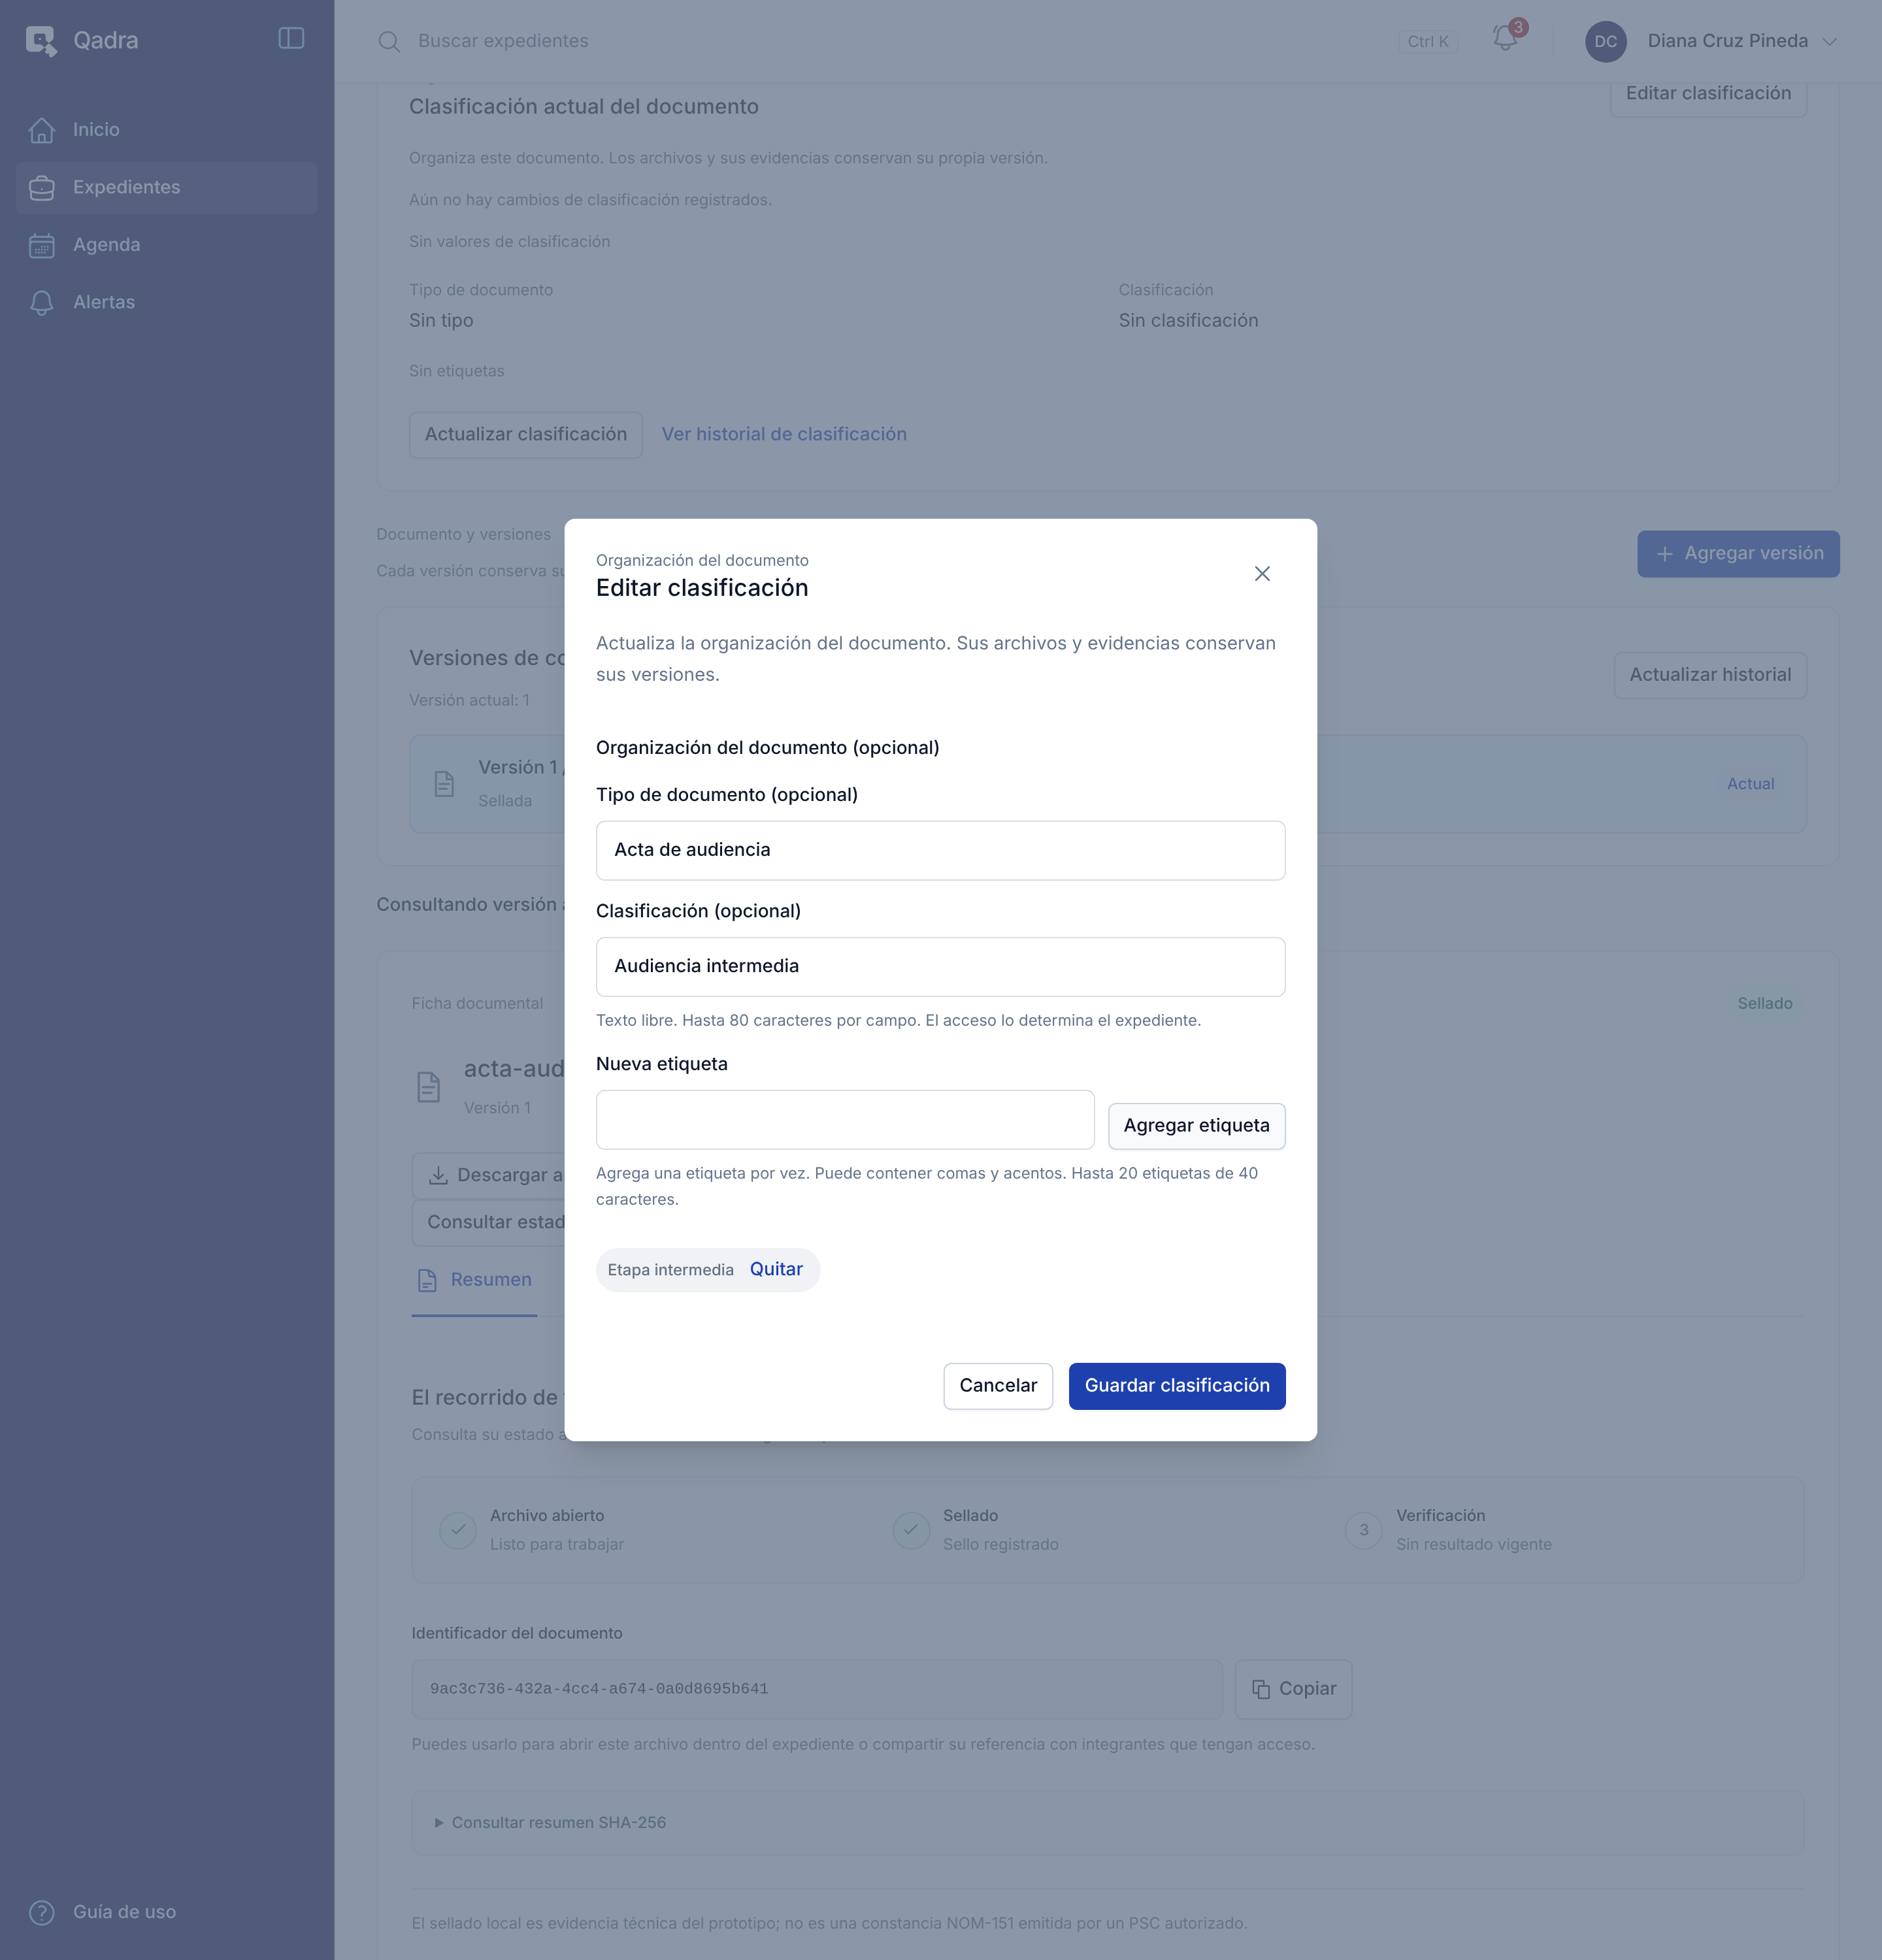
\includegraphics[width=0.9\textwidth]{capturas/A-21-editar-clasificacion.png}
  \caption{Clasificación de un documento.}
  \label{fig:manual-editar-clasificacion}
\end{figure}

\resultado La ficha muestra los valores nuevos. Para ver los cambios
anteriores, haga clic en \textbf{Ver historial de clasificación}.

\nota{Cambiar la clasificación no modifica el archivo, su firma ni su sello.
Si otra persona la cambió al mismo tiempo, Qadra le pide comparar los
valores actuales antes de guardar.}

% ---------------------------------------------------------------------
\section{Agregar una versión}\label{sec:agregar-version}

\paraque Guarda un archivo actualizado en el mismo documento sin borrar las
versiones anteriores ni su evidencia.

\disponible Administrador, Litigante y Asistente legal. El expediente debe
estar activo.

\pasos
\begin{enumerate}
  \item En la ficha del documento, haga clic en \textbf{Agregar versión}.
  \item Seleccione o arrastre el archivo en
        \textbf{Archivo de la nueva versión}.
  \item Revise el \textbf{Nombre de la nueva versión}.
  \item Haga clic en \textbf{Guardar nueva versión}.
\end{enumerate}

\begin{figure}[H]
  \centering
  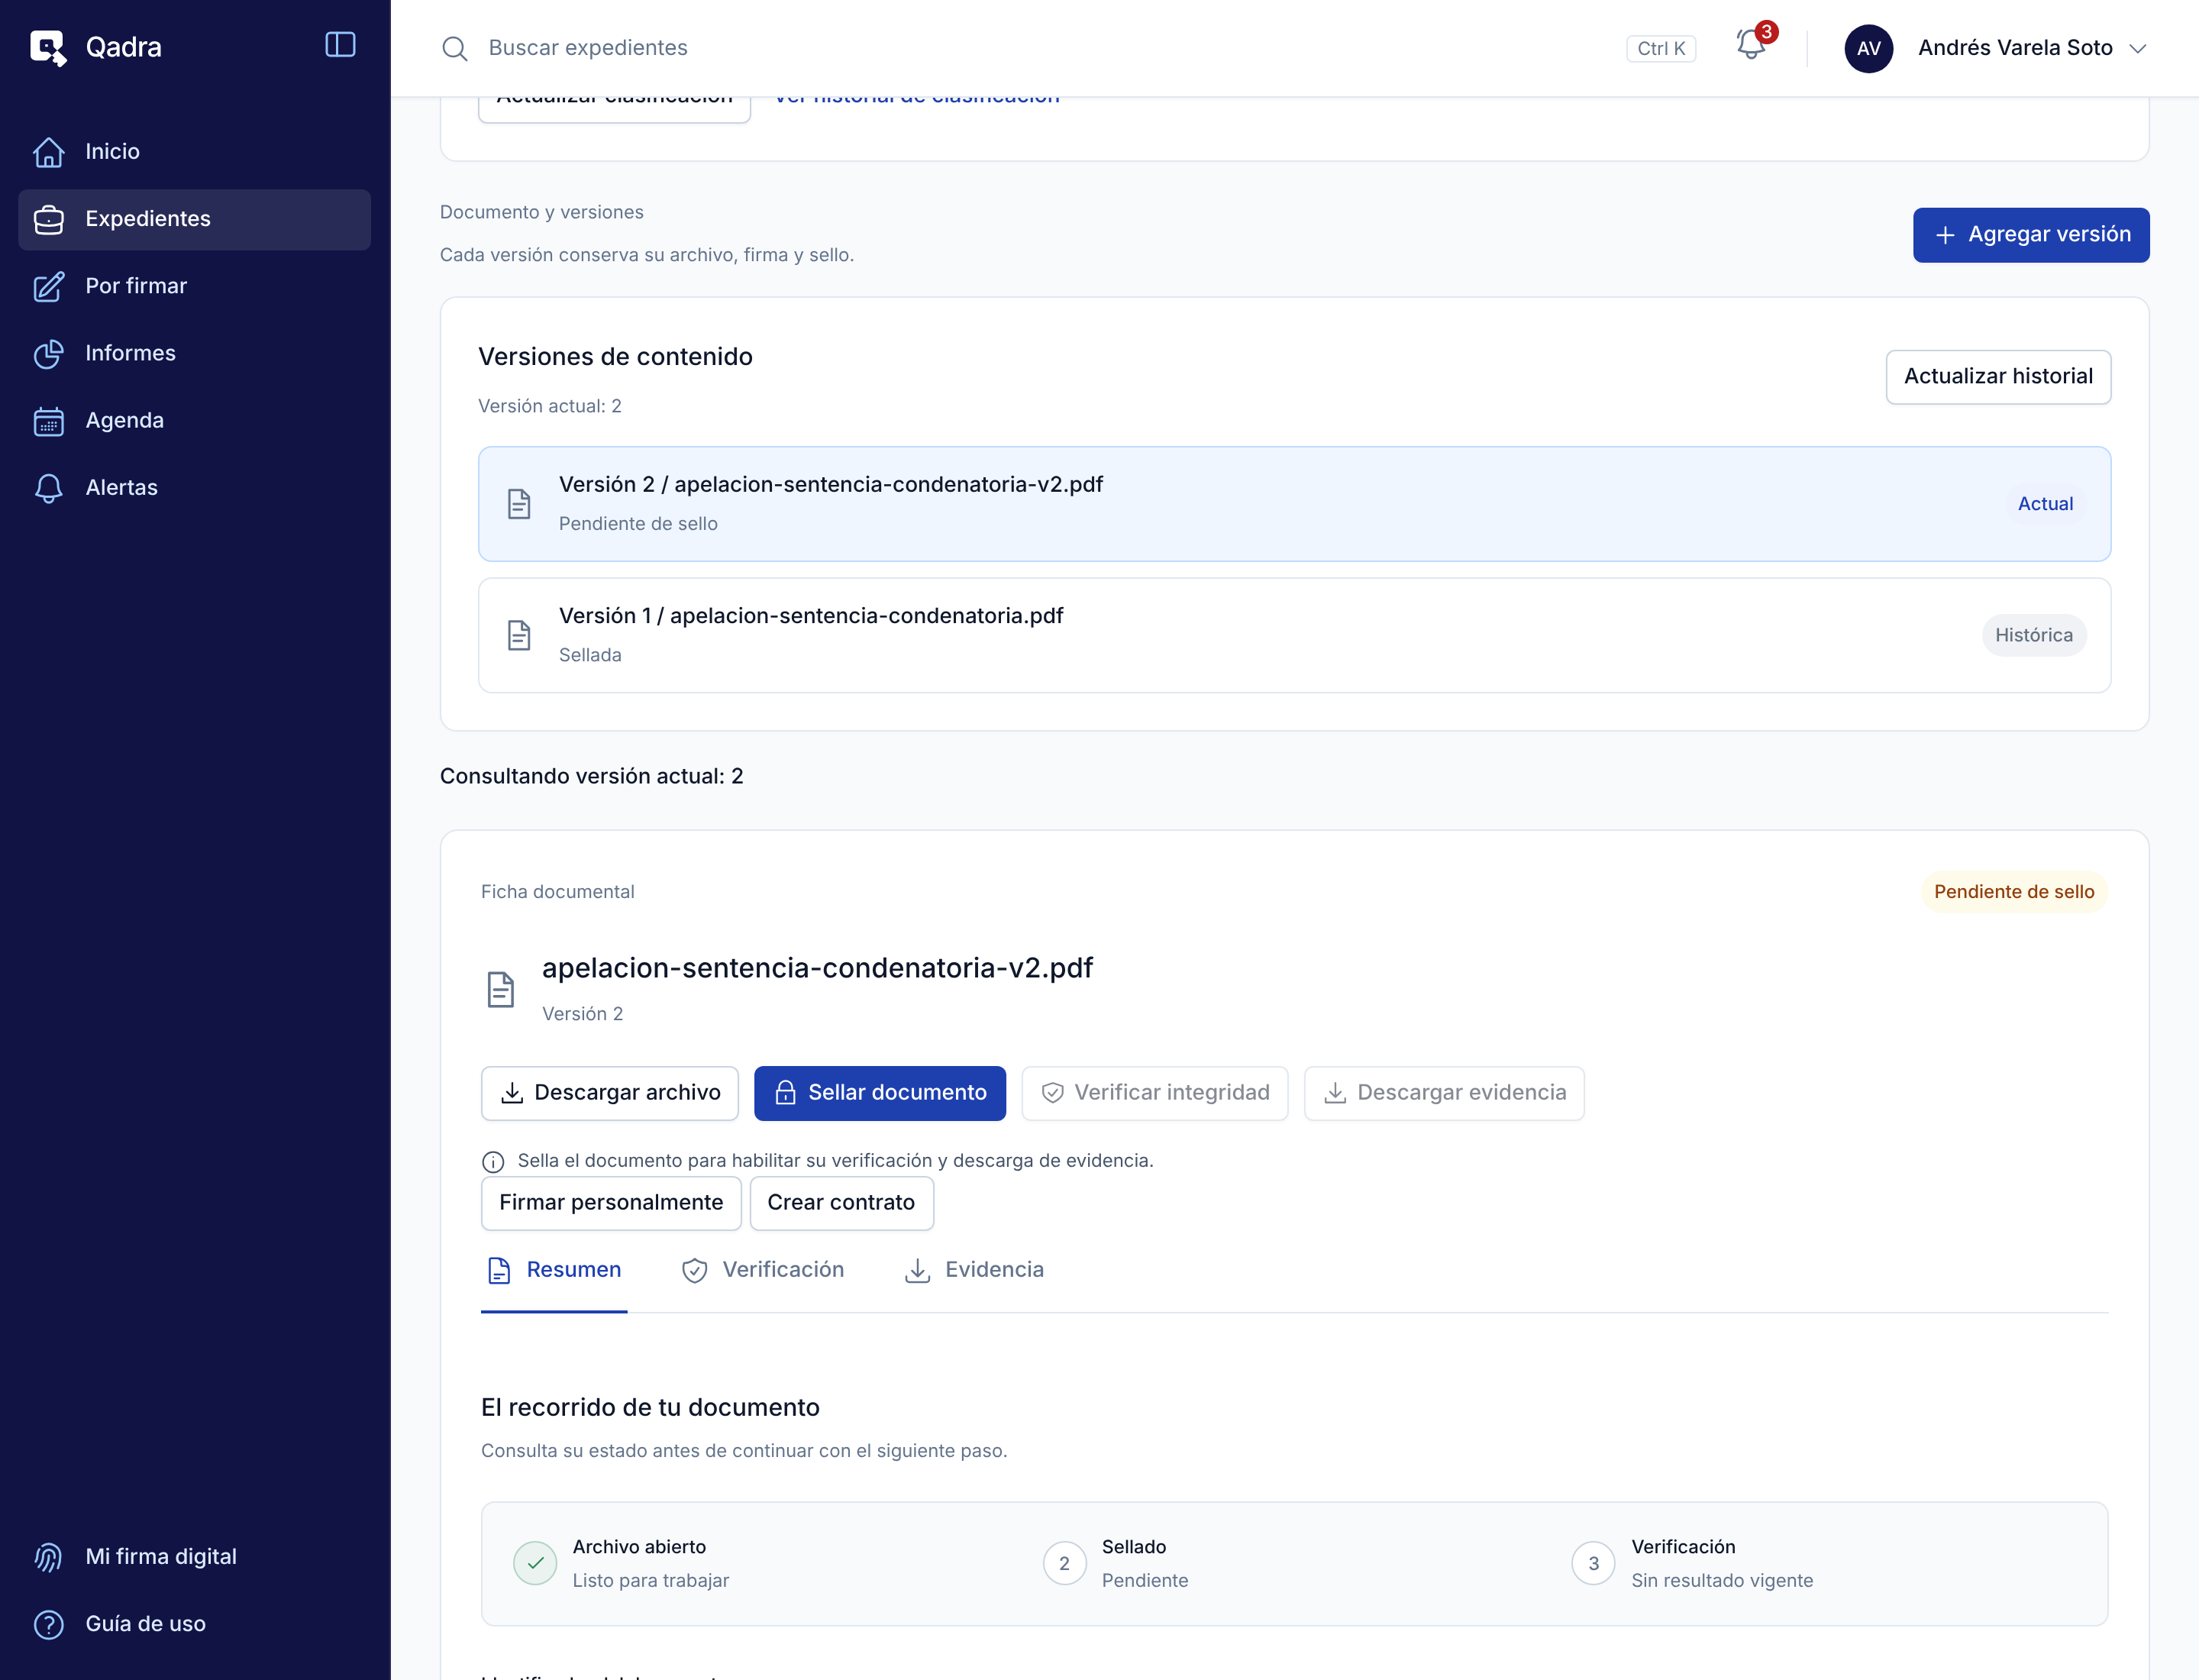
\includegraphics[width=0.9\textwidth]{capturas/A-22-versiones.png}
  \caption{Historial de versiones de un documento.}
  \label{fig:manual-versiones}
\end{figure}

\resultado La nueva versión aparece como \textbf{Actual} en
\textbf{Versiones de contenido}; las anteriores quedan como
\textbf{Histórica}.

\begin{itemize}
  \item Para trabajar con una versión anterior, haga clic en su fila. Las
        acciones de la ficha (descargar, sellar, verificar) se aplican a la
        versión elegida.
  \item Si otra persona agregó una versión mientras usted preparaba la suya,
        aparece \enquote{El documento cambió mientras preparabas el archivo.}
        Haga clic en \textbf{Consultar versión actual}, revise y confirme de
        nuevo. Su archivo se conserva.
\end{itemize}

% ---------------------------------------------------------------------
\section{Sellar un documento}\label{sec:sellar-documento}

\paraque Registra la firma del servidor y el sello de tiempo de la versión,
con su identidad. Después podrá verificarla y descargar su evidencia.

\disponible Administrador y Litigante. El expediente debe estar activo.

\importante{El sellado no se puede deshacer desde Qadra. Revise que la
versión elegida sea la correcta antes de confirmar.}

\pasos
\begin{enumerate}
  \item En la ficha del documento, elija la versión que desea sellar.
  \item Haga clic en \textbf{Sellar documento}.
  \item Lea el aviso \textbf{¿Registrar el sello del servidor?} y haga clic
        en \textbf{Confirmar sellado}.
\end{enumerate}

\begin{figure}[H]
  \centering
  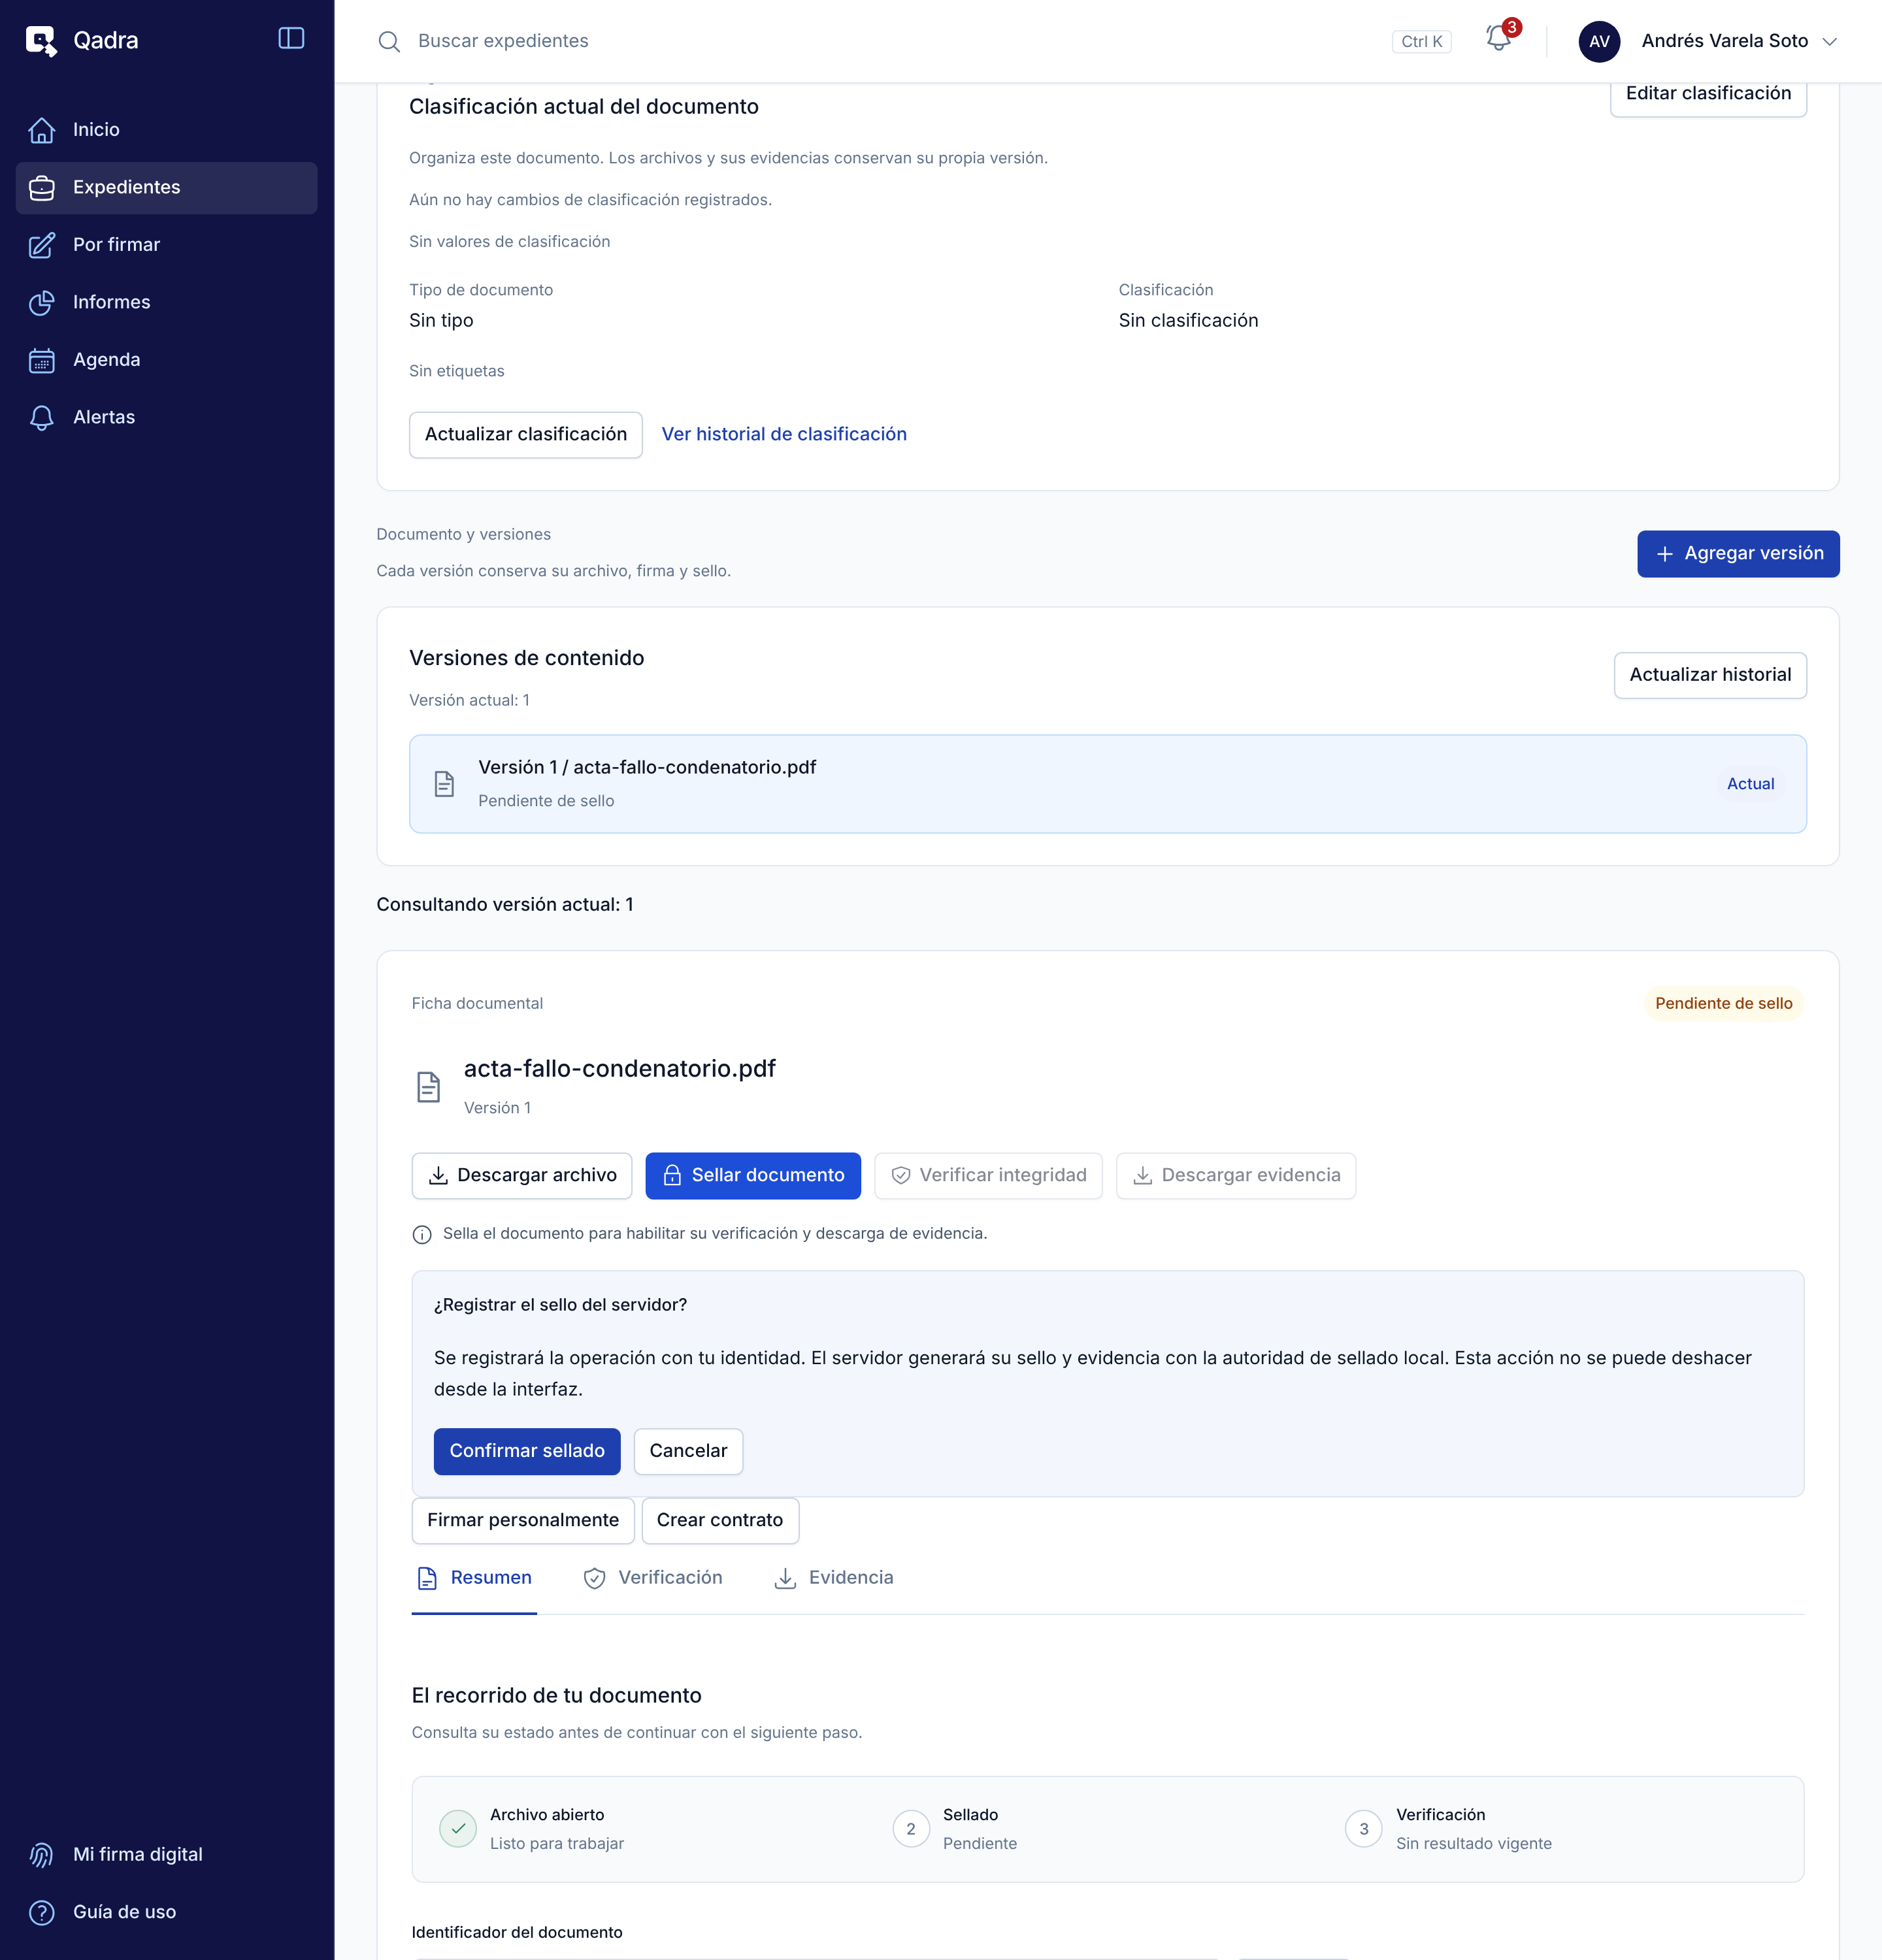
\includegraphics[width=0.9\textwidth]{capturas/A-23-sellar-documento.png}
  \caption{Confirmación del sellado.}
  \label{fig:manual-sellar-documento}
\end{figure}

\resultado Aparece \enquote{Documento sellado correctamente.} y el estado
cambia a \textbf{Sellado}.

\begin{itemize}
  \item \textbf{Resultado incierto:} si se pierde la conexión, aparece
        \enquote{El resultado del sellado es incierto. Consulta esta versión
        antes de otra decisión.} Haga clic en
        \textbf{Consultar estado del sellado}. Selle de nuevo solo si
        aparece \enquote{Esta versión sigue sin sello. Puedes iniciar una
        nueva confirmación.}
  \item El Asistente legal ve \enquote{Solicita al administrador o a un
        litigante que selle el documento para verificarlo o descargar su
        evidencia.}
\end{itemize}

% ---------------------------------------------------------------------
\section{Verificar un documento}\label{sec:verificar-documento}

\paraque Comprueba que el archivo sellado no cambió y que su firma, su
certificado y su sello de tiempo son correctos.

\disponible Administrador, Litigante y Asistente legal. La versión debe
estar sellada.

\pasos
\begin{enumerate}
  \item En la ficha del documento, haga clic en
        \textbf{Verificar integridad}.
  \item Abra la pestaña \textbf{Verificación} y revise el
        \textbf{Resultado de verificación}.
\end{enumerate}

\begin{figure}[H]
  \centering
  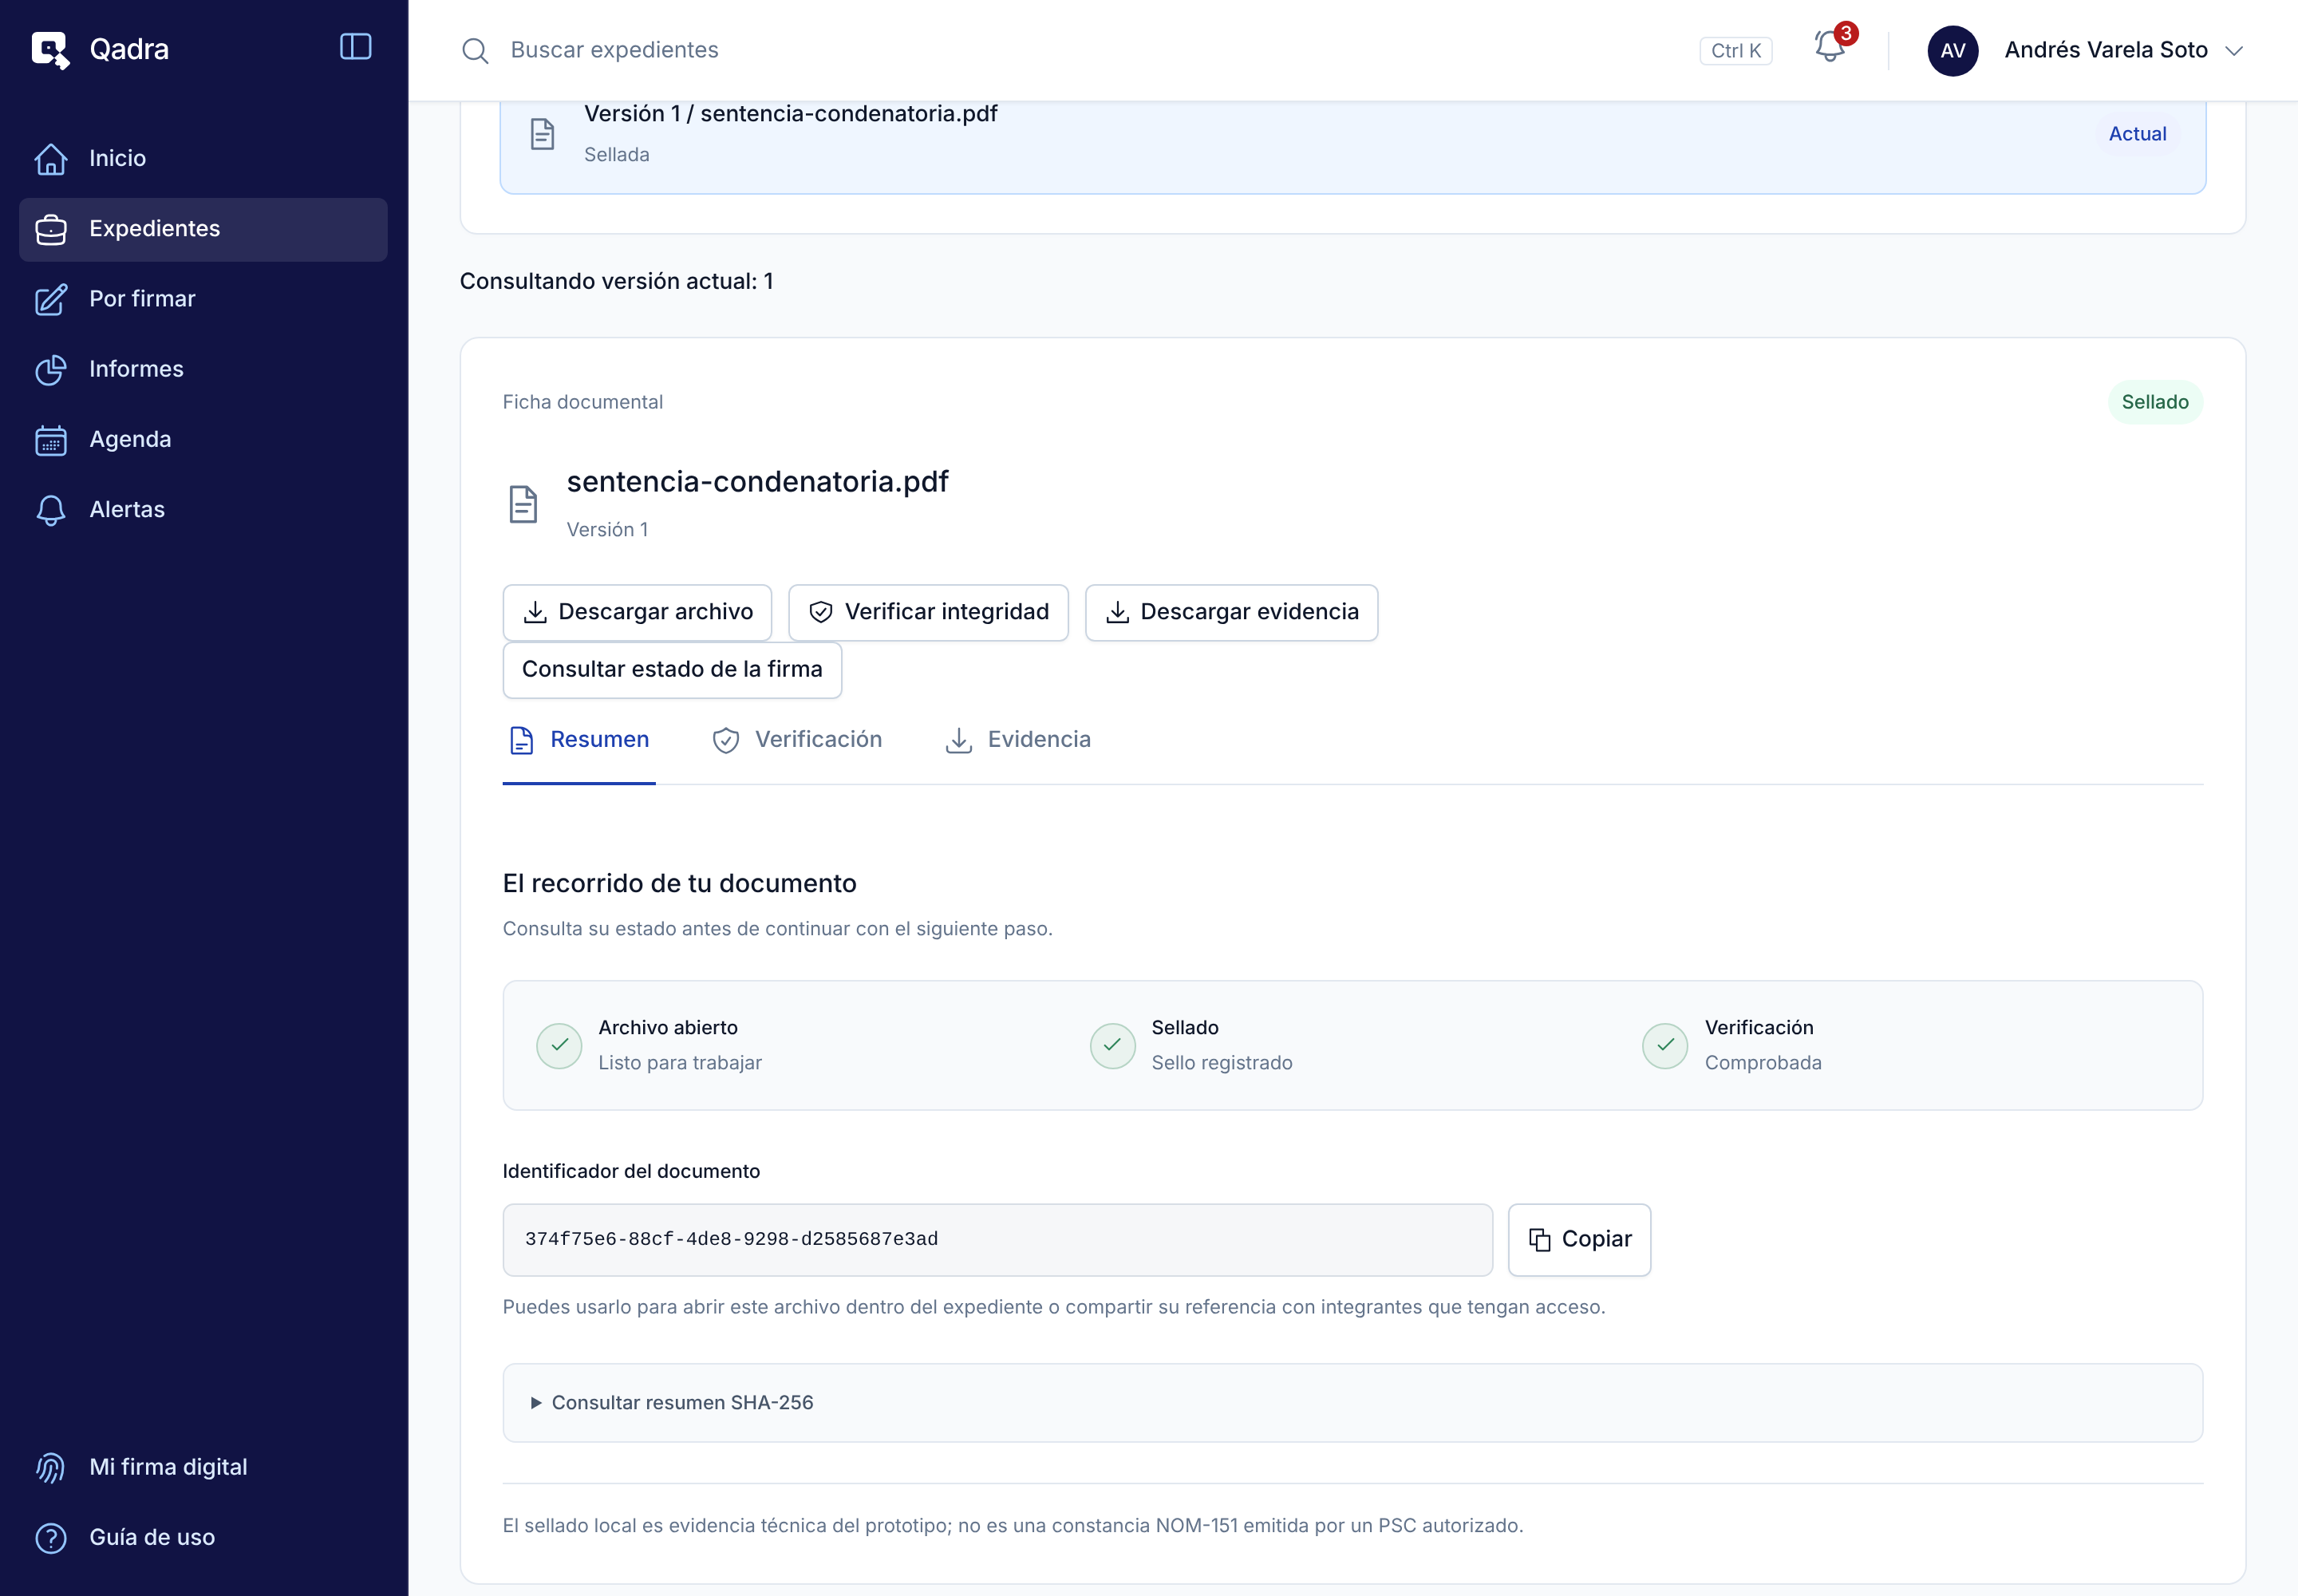
\includegraphics[width=0.9\textwidth]{capturas/A-24-resultado-verificacion.png}
  \caption{Resultado de la verificación.}
  \label{fig:manual-resultado-verificacion}
\end{figure}

\resultado Aparece \textbf{Verificación válida} con las cuatro
comprobaciones en \textbf{Correcto}.

\begin{table}[H]
  \centering
  \caption{Comprobaciones de la verificación.}\label{tab:comprobaciones}
  \begin{tabularx}{\textwidth}{L{4.2cm} Y}
    \toprule
    \textbf{Comprobación} & \textbf{Cuando está \textbf{Correcto}} \\
    \midrule
    \textbf{Integridad del archivo}    & El archivo no cambió desde que se selló. \\
    \textbf{Firma digital}             & La firma corresponde al archivo. \\
    \textbf{Certificado y revocación}  & El certificado es válido y no está revocado. \\
    \textbf{Sello de tiempo}           & El sello de tiempo corresponde al archivo. \\
    \bottomrule
  \end{tabularx}
\end{table}

\importante{Si alguna comprobación muestra \textbf{Revisar}, el resultado es
\textbf{Verificación no válida} y el documento aparece como
\textbf{Revisar evidencia}. No use esa evidencia: avise al Administrador y
consulte \textbf{Ver detalles técnicos de la verificación}.}

% ---------------------------------------------------------------------
\section{Descargar y validar la evidencia}\label{sec:descargar-evidencia}

\paraque Descarga un paquete ZIP con el documento y todo lo necesario para
comprobarlo fuera de Qadra.

\disponible Administrador, Litigante y Asistente legal. La versión debe
estar sellada.

\pasos
\begin{enumerate}
  \item En la ficha del documento, haga clic en
        \textbf{Descargar evidencia}.
  \item Guarde el archivo \texttt{evidencia-[identificador]-v[versión].zip}
        sin descomprimirlo ni modificarlo.
  \item Para validarlo en el navegador, abra la pestaña \textbf{Evidencia}.
        En \textbf{Validar un paquete de evidencia}, seleccione el ZIP en
        \textbf{Paquete de evidencia (ZIP)} y haga clic en
        \textbf{Validar paquete}.
\end{enumerate}

\begin{figure}[H]
  \centering
  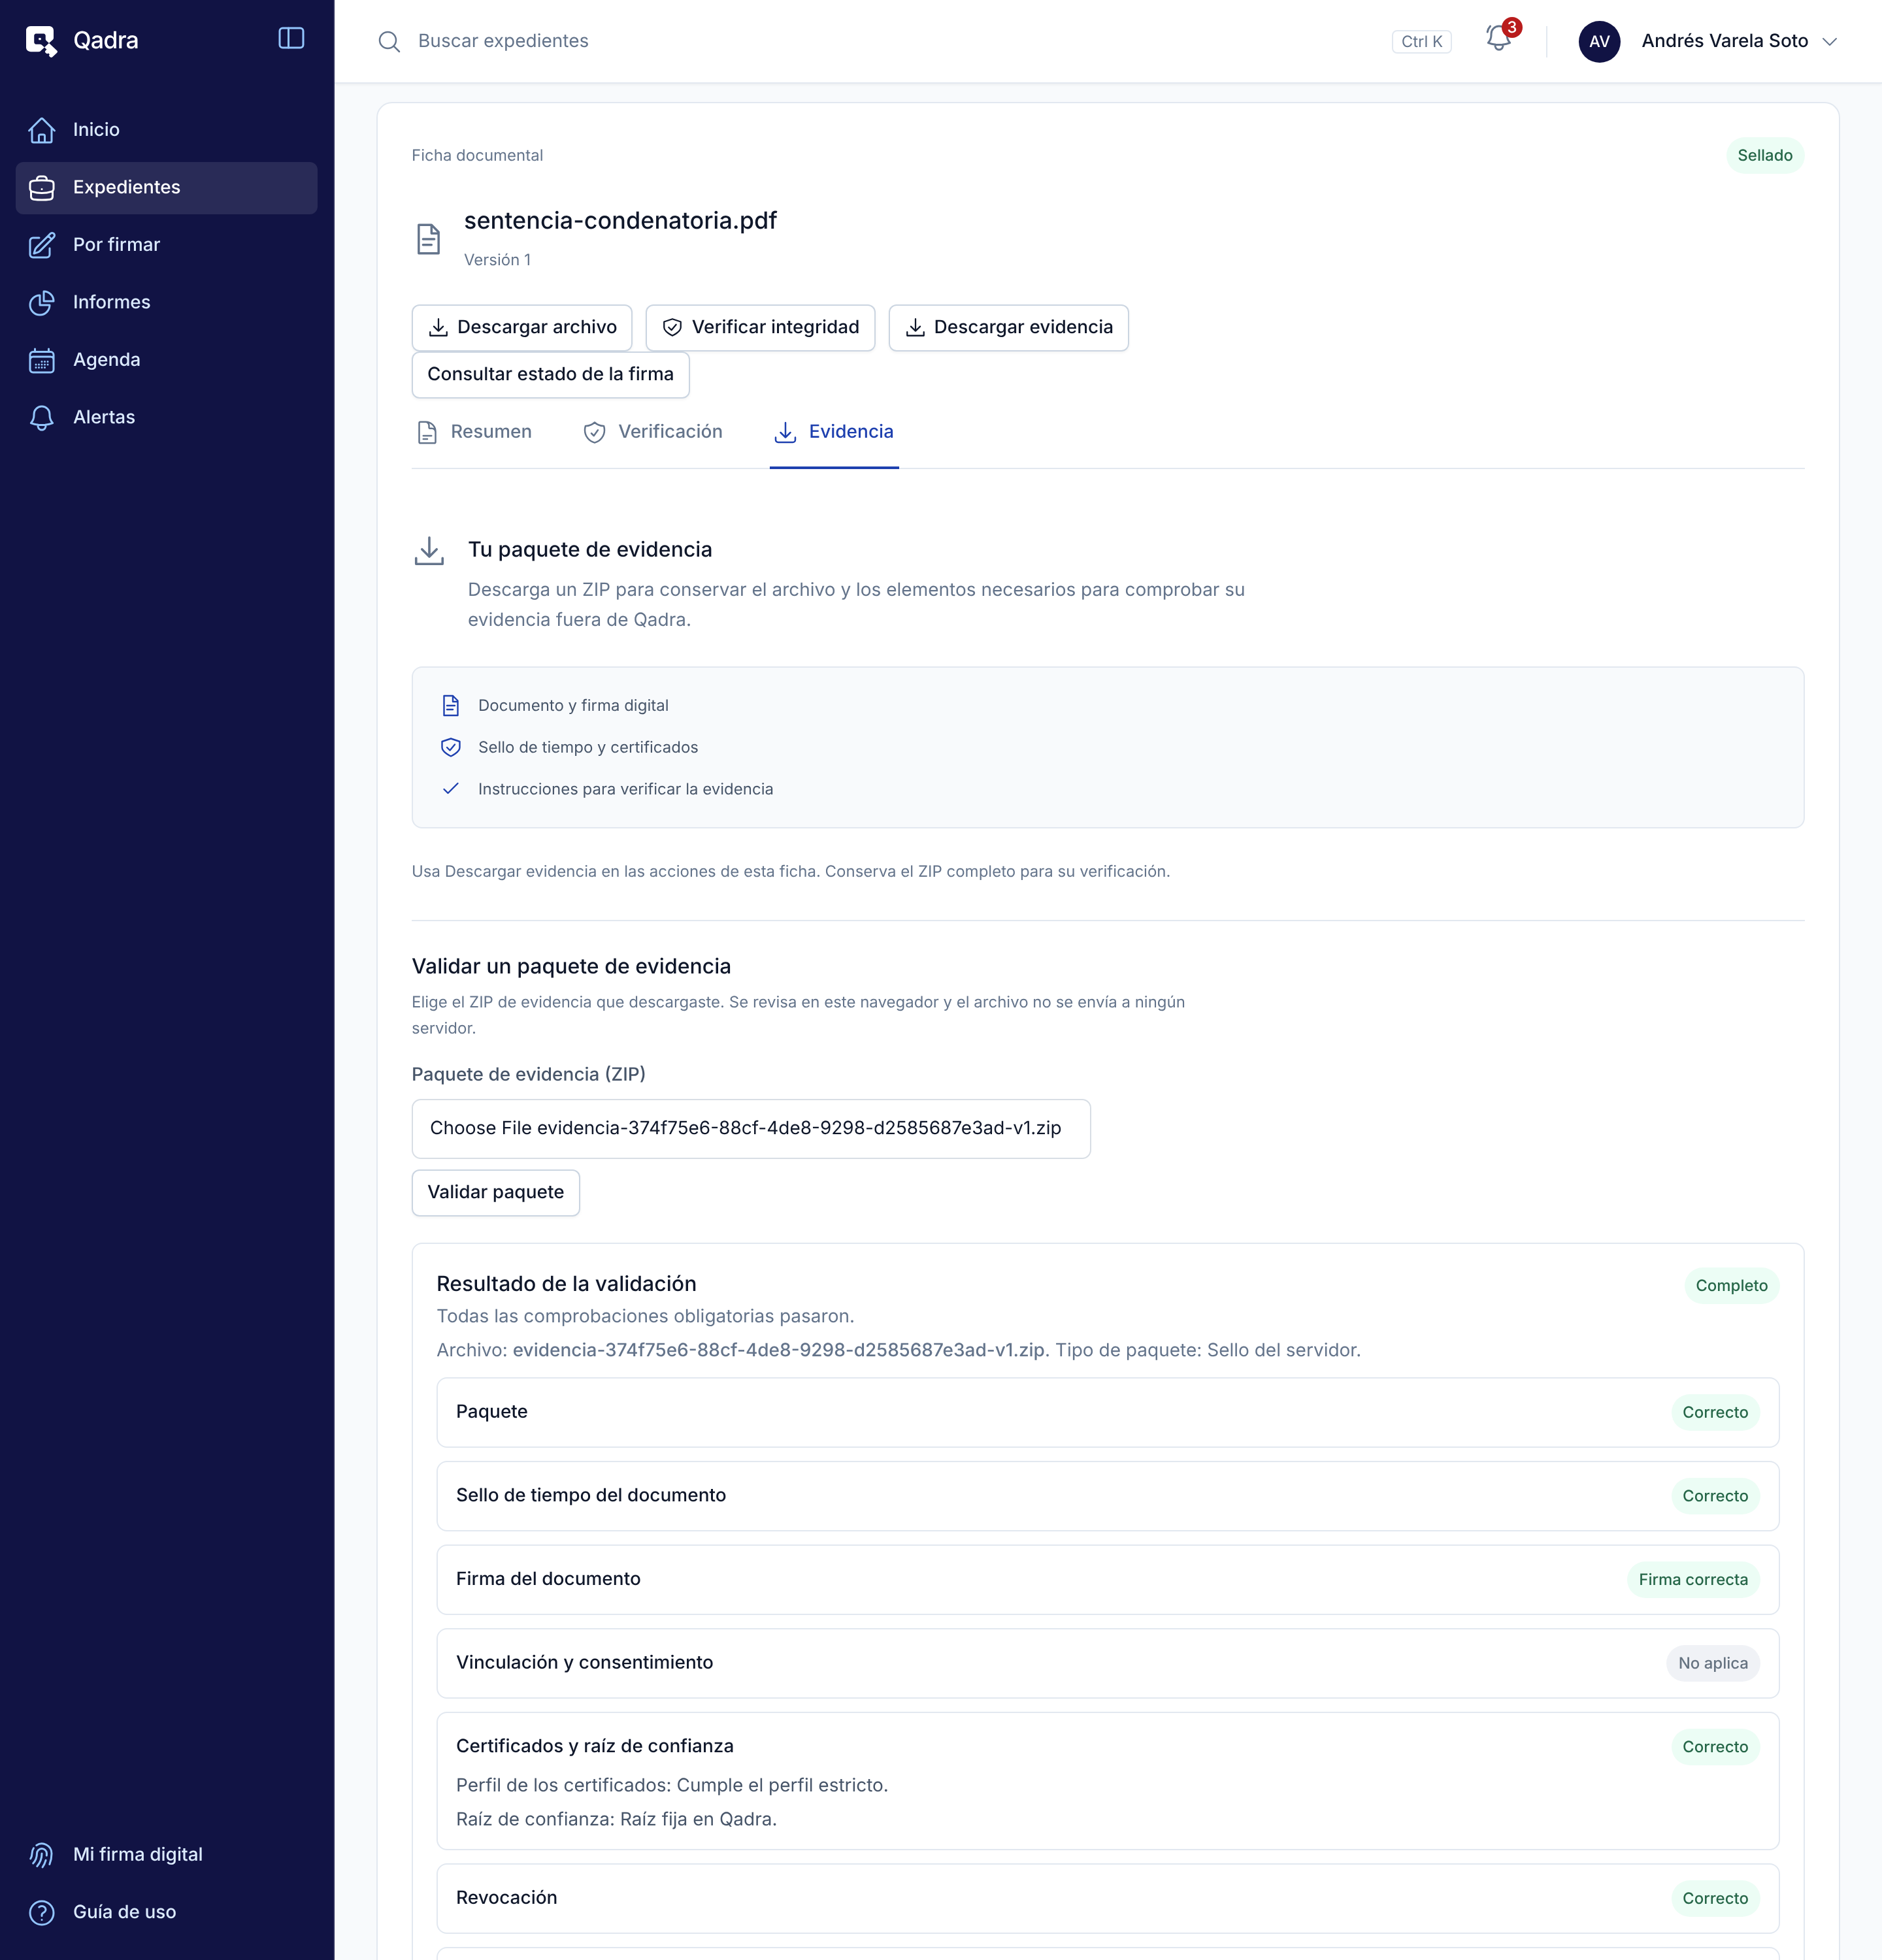
\includegraphics[width=0.9\textwidth]{capturas/A-25-evidencia.png}
  \caption{Paquete de evidencia y su validación.}
  \label{fig:manual-evidencia}
\end{figure}

\resultado Aparece \enquote{Evidencia descargada.} Al validarlo, el resultado
\textbf{Completo} indica que todas las comprobaciones obligatorias pasaron.

\begin{itemize}
  \item El paquete contiene el documento y su firma, el sello de tiempo, los
        certificados y las instrucciones para verificarlo.
  \item La validación se hace en su navegador; el archivo no se envía a
        ningún servidor.
  \item Los resultados posibles de la validación se explican en la \cref{tab:resultado-validacion}.
        Cualquier persona puede verificar el ZIP sin cuenta, siguiendo la
        verificación independiente del \cref{cap:verificacion-independiente}.
\end{itemize}

% ---------------------------------------------------------------------
\section{Firmar personalmente un documento}\label{sec:firma-personal}

\paraque Firma una versión PDF con su propio certificado, en lugar del sello
del servidor.

\disponible Litigante, con un certificado vinculado en
\textbf{Mi firma digital}. La versión debe ser PDF, no estar sellada ni en
contrato, y el expediente debe estar activo.

Tenga a la mano su clave privada cifrada (archivo \texttt{.pem}) y su
contraseña.

\pasos
\begin{enumerate}
  \item En la ficha del documento, haga clic en
        \textbf{Firmar personalmente}.
  \item Haga clic en \textbf{Revisar PDF} y lea el documento.
  \item Marque \textbf{He revisado este PDF y confirmo su contenido}.
  \item En \textbf{Firmar en este dispositivo}, seleccione su
        \textbf{Clave privada cifrada}, escriba la
        \textbf{Contraseña de la clave} y haga clic en
        \textbf{Firmar localmente}.
  \item Haga clic en \textbf{Preparar consentimiento}.
  \item Marque \textbf{Confirmo firmar esta versión con mi certificado} y
        firme de nuevo con \textbf{Firmar localmente}.
  \item Haga clic en \textbf{Enviar firma personal}.
\end{enumerate}

\begin{figure}[H]
  \centering
  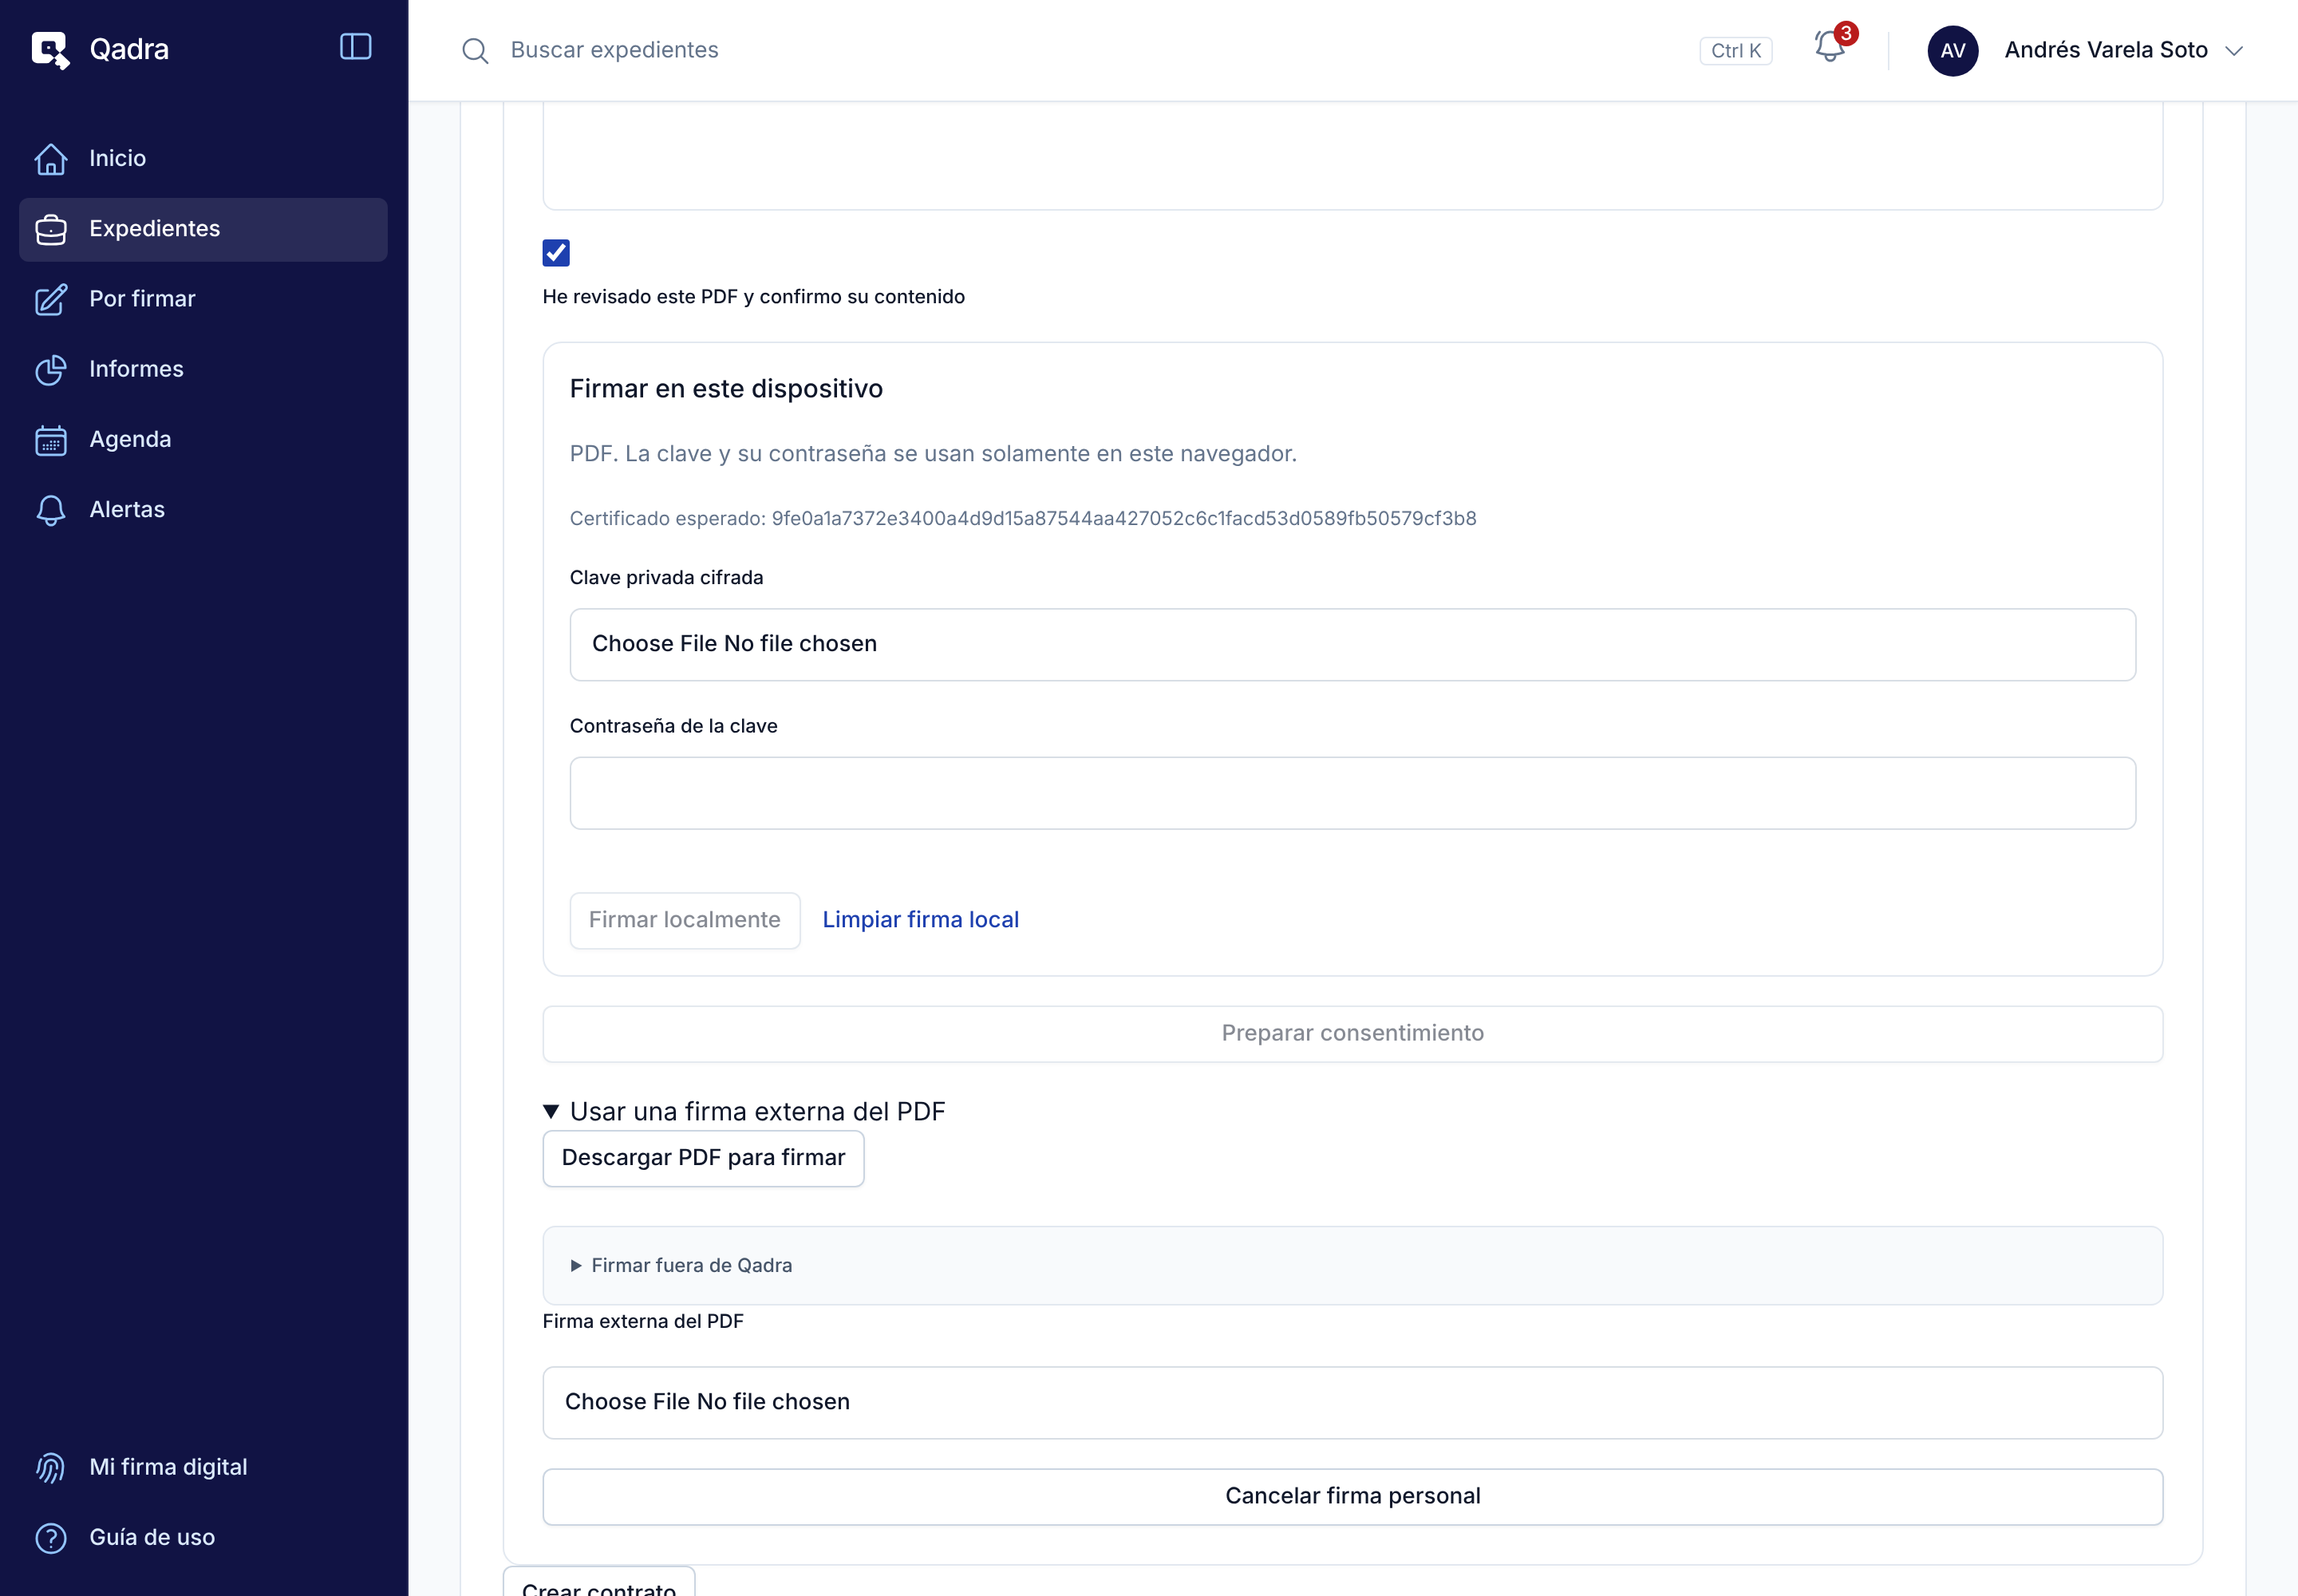
\includegraphics[width=0.9\textwidth]{capturas/A-26-firma-personal.png}
  \caption{Firma personal de un documento.}
  \label{fig:manual-firma-personal}
\end{figure}

\resultado Aparece \textbf{Firma personal aceptada} y la versión queda
\textbf{Sellado}. Haga clic en \textbf{Descargar recibo de firma} para
conservar el recibo.

\begin{itemize}
  \item Si no tiene certificado vinculado, aparece \enquote{Primero registra
        tu certificado en Mi firma digital.}
  \item Para firmar con su propia herramienta, use
        \textbf{Usar una firma externa del PDF} y
        \textbf{Usar una firma externa del consentimiento}.
  \item Si se pierde la respuesta, haga clic en
        \textbf{Consultar recibo de firma}; consultar no vuelve a enviar la
        firma.
  \item Para revisar después el resultado, haga clic en
        \textbf{Consultar estado de la firma}.
\end{itemize}

\chapter{Actividad procesal}\label{cap:actividad-procesal}

Las pestañas de este capítulo registran lo que ocurre en el procedimiento
penal. Todas funcionan igual en cuanto a permisos:

\begin{itemize}
  \item \textbf{Administrador y Litigante asignado:} registran, corrigen y
        retiran.
  \item \textbf{Asistente legal asignado:} solo consulta y revisa el
        historial.
  \item \textbf{Expediente cerrado:} se puede consultar, pero no registrar
        cambios.
\end{itemize}

\nota{Qadra conserva lo que usted declara. Registrar una audiencia, una
resolución o un plazo no acredita por sí solo un acto judicial ni sus
efectos jurídicos.}

% ---------------------------------------------------------------------
\section{Cómo funcionan los registros}\label{sec:patron-registros}

Todos los formularios de este capítulo siguen el mismo recorrido:

\begin{enumerate}
  \item Llene el formulario.
  \item Haga clic en el botón de revisión (\textbf{Revisar registro},
        \textbf{Preparar registro}, \textbf{Preparar plazo}, según la
        pantalla).
  \item Revise el resumen y haga clic en el botón de confirmación
        (\textbf{Confirmar registro}, \textbf{Confirmar plazo}, etc.).
\end{enumerate}

\begin{table}[H]
  \centering
  \caption{Situaciones comunes en los formularios.}\label{tab:situaciones-comunes}
  \begin{tabularx}{\textwidth}{L{3.6cm} Y}
    \toprule
    \textbf{Situación} & \textbf{Qué hacer} \\
    \midrule
    Historial
      & Cada registro guarda sus cambios con autor y fecha. Use los botones
        \textbf{Ver historial de\ldots} de cada pestaña. \\
    Borrador guardado
      & Si cerró un formulario sin confirmar, aparece un botón
        \textbf{Retomar borrador de\ldots} para continuar. \\
    Otra persona cambió el registro
      & Haga clic en \textbf{Comparar con el registro actual}, revise las
        diferencias y elija \textbf{Usar esta base y conservar borrador}
        antes de confirmar. \\
    Resultado incierto
      & Si se pierde la respuesta, aparece \textbf{Resultado incierto}. Haga
        clic en \textbf{Consultar envío exacto} antes de intentar otra vez;
        consultar no repite el registro. \\
    Cerrar el formulario
      & \textbf{Cerrar formulario} descarta el borrador, pero no cancela un
        envío en curso. \\
    \bottomrule
  \end{tabularx}
\end{table}

% ---------------------------------------------------------------------
\section{Participantes}\label{sec:participantes}

\paraque Directorio de las personas e instituciones que intervienen en el
expediente. Registrar a una persona no le da acceso a Qadra.

\disponible Administrador y Litigante (registran); Asistente legal
(consulta).

\begin{table}[H]
  \centering
  \caption{Acciones en Participantes.}\label{tab:acciones-participantes}
  \begin{tabularx}{\textwidth}{L{4.4cm} Y}
    \toprule
    \textbf{Botón} & \textbf{Qué hace} \\
    \midrule
    \textbf{Agregar participante}     & Registra una identidad y su rol en el expediente. \\
    \textbf{Registrar ficha pendiente}& Registro manual rápido, para completarlo después. \\
    \textbf{Completar perfil}         & Convierte una ficha pendiente en un perfil completo. \\
    \textbf{Editar participante}      & Corrige los datos; la versión anterior queda en el historial. \\
    \textbf{Archivar participante} / \textbf{Reactivar participante}
                                      & Ordena el directorio; no cambia la situación jurídica. \\
    \textbf{Ver historial de cambios} & Muestra todas las versiones del registro. \\
    \bottomrule
  \end{tabularx}
\end{table}

\pasos\ Agregar un participante:
\begin{enumerate}
  \item En la pestaña \textbf{Participantes}, haga clic en
        \textbf{Agregar participante}.
  \item En \textbf{Datos de identidad}, elija el \textbf{Tipo de identidad}
        (\textbf{Persona} u \textbf{Órgano institucional}) y escriba el
        \textbf{Nombre de la persona}.
  \item En \textbf{Ficha de participación}, elija el
        \textbf{Tipo de participante} y llene los campos que aparezcan.
  \item Haga clic en \textbf{Revisar identidad y coincidencias}. Si Qadra
        encuentra personas parecidas, elija
        \textbf{Elegir identidad existente}, \textbf{Registrar otra identidad}
        o \textbf{Declarar persona distinta}.
  \item Haga clic en \textbf{Preparar registro} y después en
        \textbf{Confirmar registro}.
\end{enumerate}

\begin{figure}[H]
  \centering
  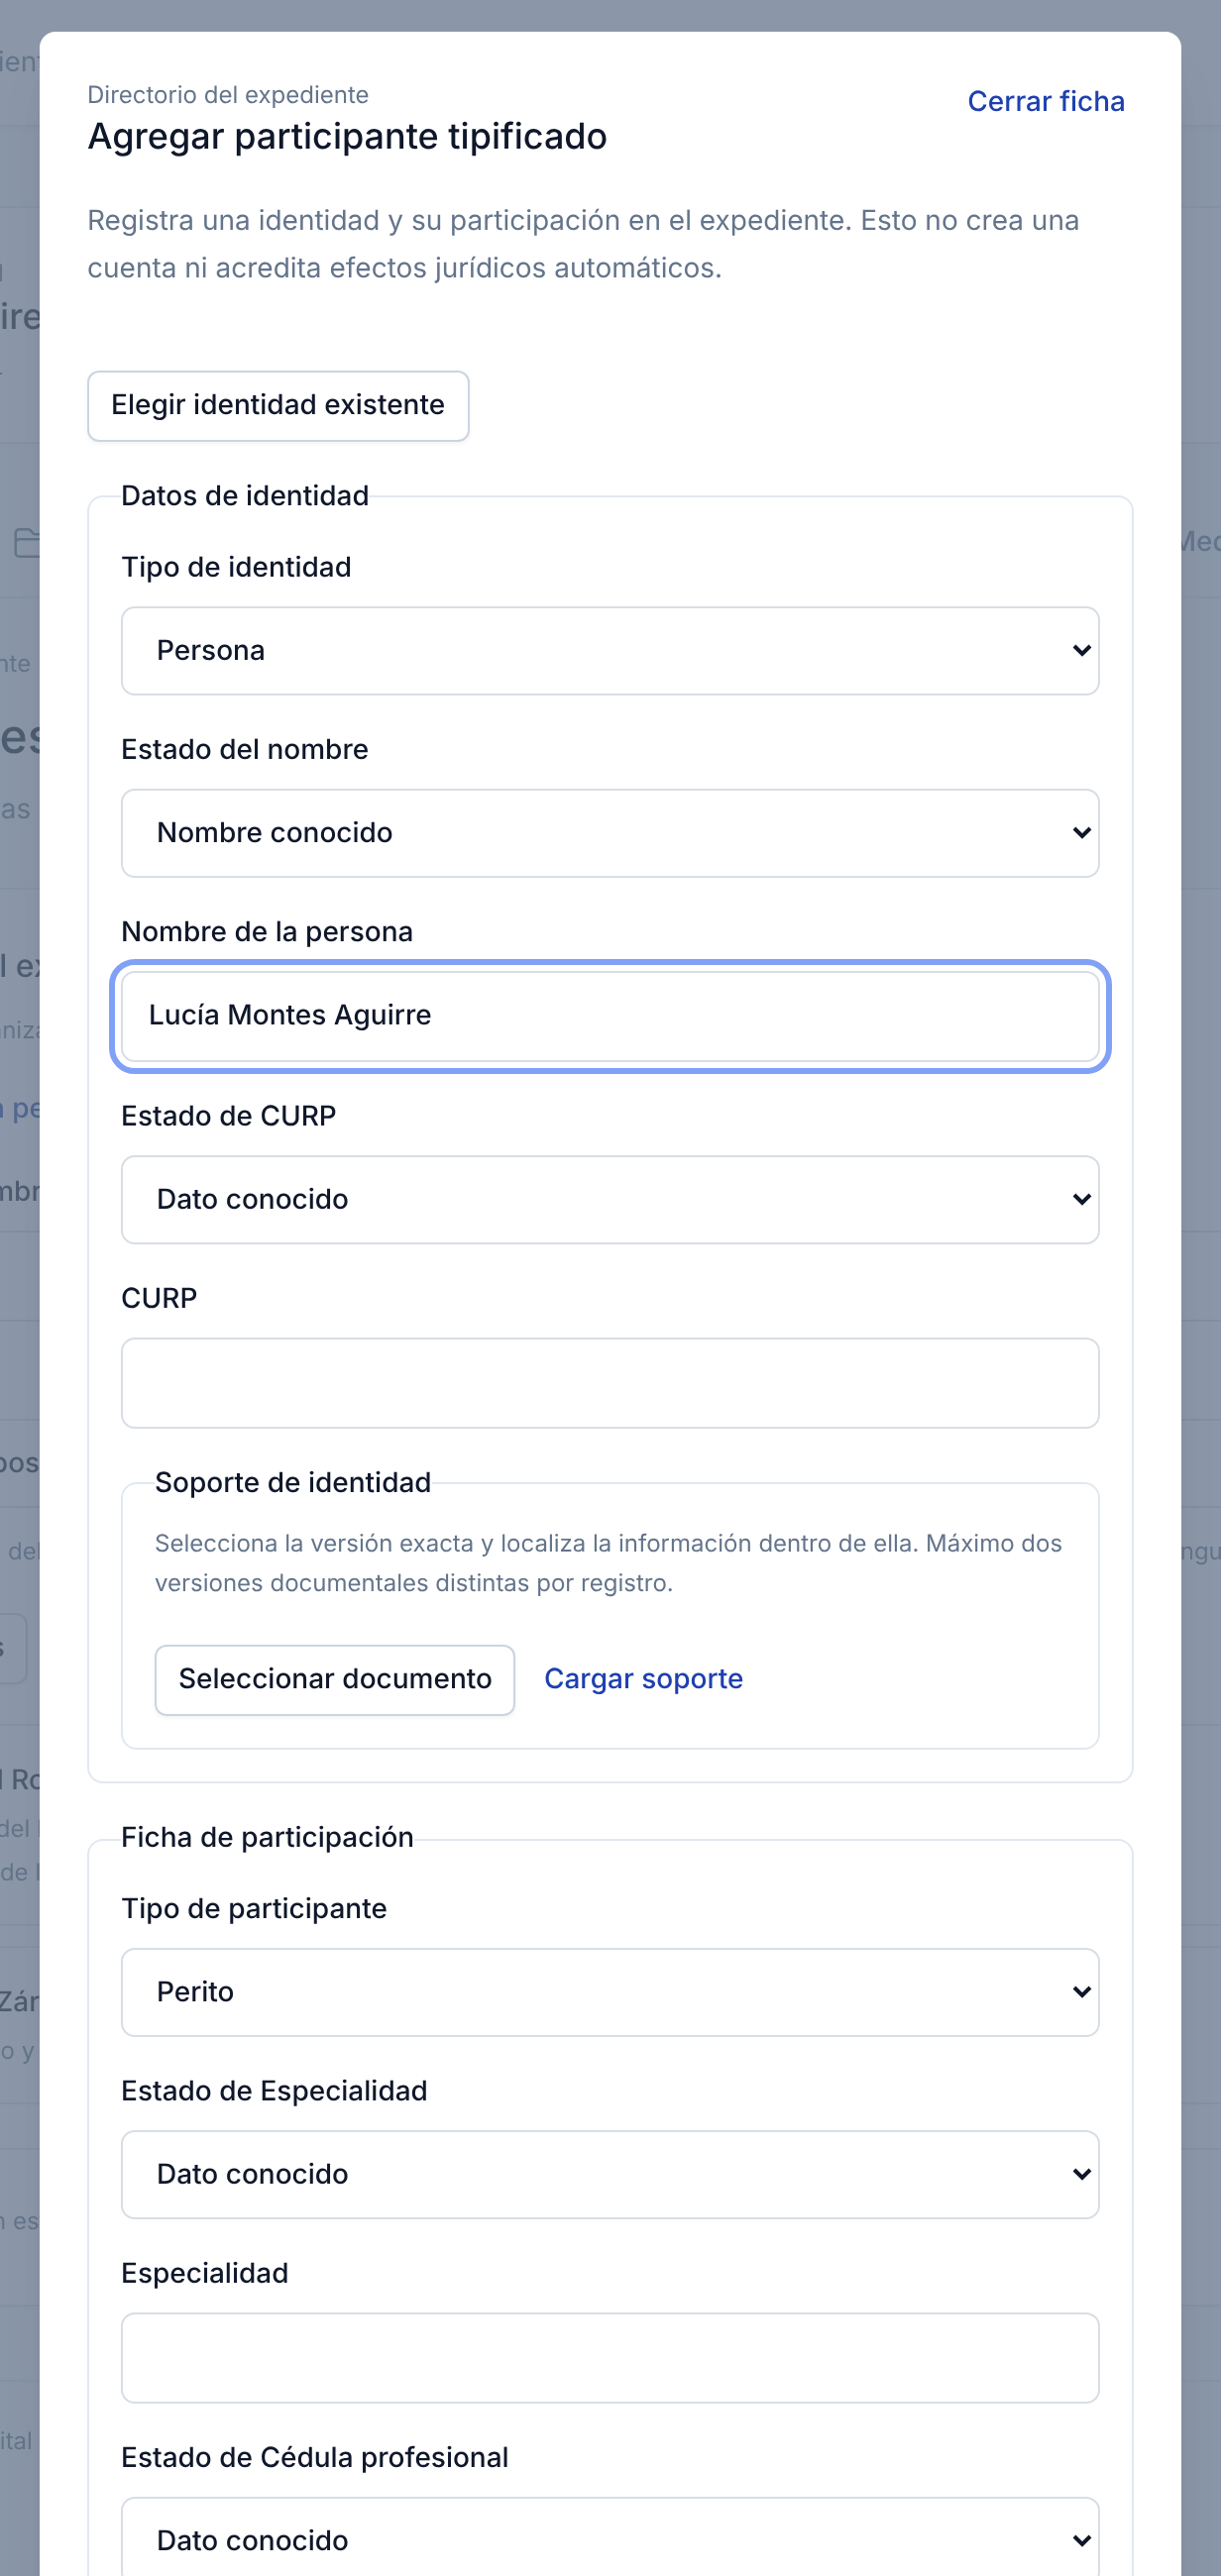
\includegraphics[width=0.9\textwidth,height=0.8\textheight,keepaspectratio]{capturas/A-27-agregar-participante.png}
  \caption{Registro de un participante.}
  \label{fig:manual-agregar-participante}
\end{figure}

\resultado El participante aparece en el \textbf{Directorio del expediente}.

\begin{itemize}
  \item Tipos disponibles: Imputado, Víctima u ofendido, Defensor,
        Ministerio Público, Asesor jurídico, Juez de control, Tribunal de
        enjuiciamiento, Perito, Policía, Supervisión de medidas cautelares y
        Otro.
  \item \textbf{Defensor} y \textbf{Juez de control} requieren certificado y
        firma: descargue la declaración con
        \textbf{Descargar declaración binaria}, fírmela con su herramienta y
        cargue el certificado y la firma con \textbf{Elegir certificado} y
        \textbf{Elegir firma}. Su clave privada nunca se sube a Qadra.
  \item Qadra nunca une a dos personas solo porque tengan el mismo nombre;
        usted decide en la revisión de coincidencias.
\end{itemize}

% ---------------------------------------------------------------------
\section{Etapas}\label{sec:etapas}

\paraque Registra la etapa procesal actual (Investigación, Intermedia o
Juicio) y sus cambios, con el documento que los respalda.

\disponible Administrador y Litigante (registran); Asistente legal
(consulta). Requiere la ficha penal completa.

\begin{table}[H]
  \centering
  \caption{Acciones en Etapas.}\label{tab:acciones-etapas}
  \begin{tabularx}{\textwidth}{L{4.6cm} Y}
    \toprule
    \textbf{Botón} & \textbf{Qué hace} \\
    \midrule
    \textbf{Registrar etapa actual}       & Declara la etapa en la que se encuentra un expediente sin etapa registrada. \\
    \textbf{Registrar paso a Intermedia}  & Registra el paso desde Investigación, con la acusación. \\
    \textbf{Registrar paso a Juicio}      & Registra el paso desde Intermedia, con el auto de apertura y su recepción. \\
    \textbf{Ver historial de etapas}      & Muestra todas las etapas registradas. \\
    \bottomrule
  \end{tabularx}
\end{table}

\pasos\ Registrar el paso a la siguiente etapa:
\begin{enumerate}
  \item En la pestaña \textbf{Etapas}, haga clic en
        \textbf{Registrar paso a Intermedia} (o
        \textbf{Registrar paso a Juicio}).
  \item Indique la fecha (por ejemplo, \textbf{Fecha de la acusación}). Si
        no conoce la hora, elija \textbf{Fecha sin hora conocida}.
  \item Elija el documento de soporte con \textbf{Elegir documento}, o
        súbalo con \textbf{Cargar soporte}. Debe ser PDF o DOCX.
  \item Haga clic en \textbf{Revisar registro} y después en
        \textbf{Registrar transición}.
\end{enumerate}

\begin{figure}[H]
  \centering
  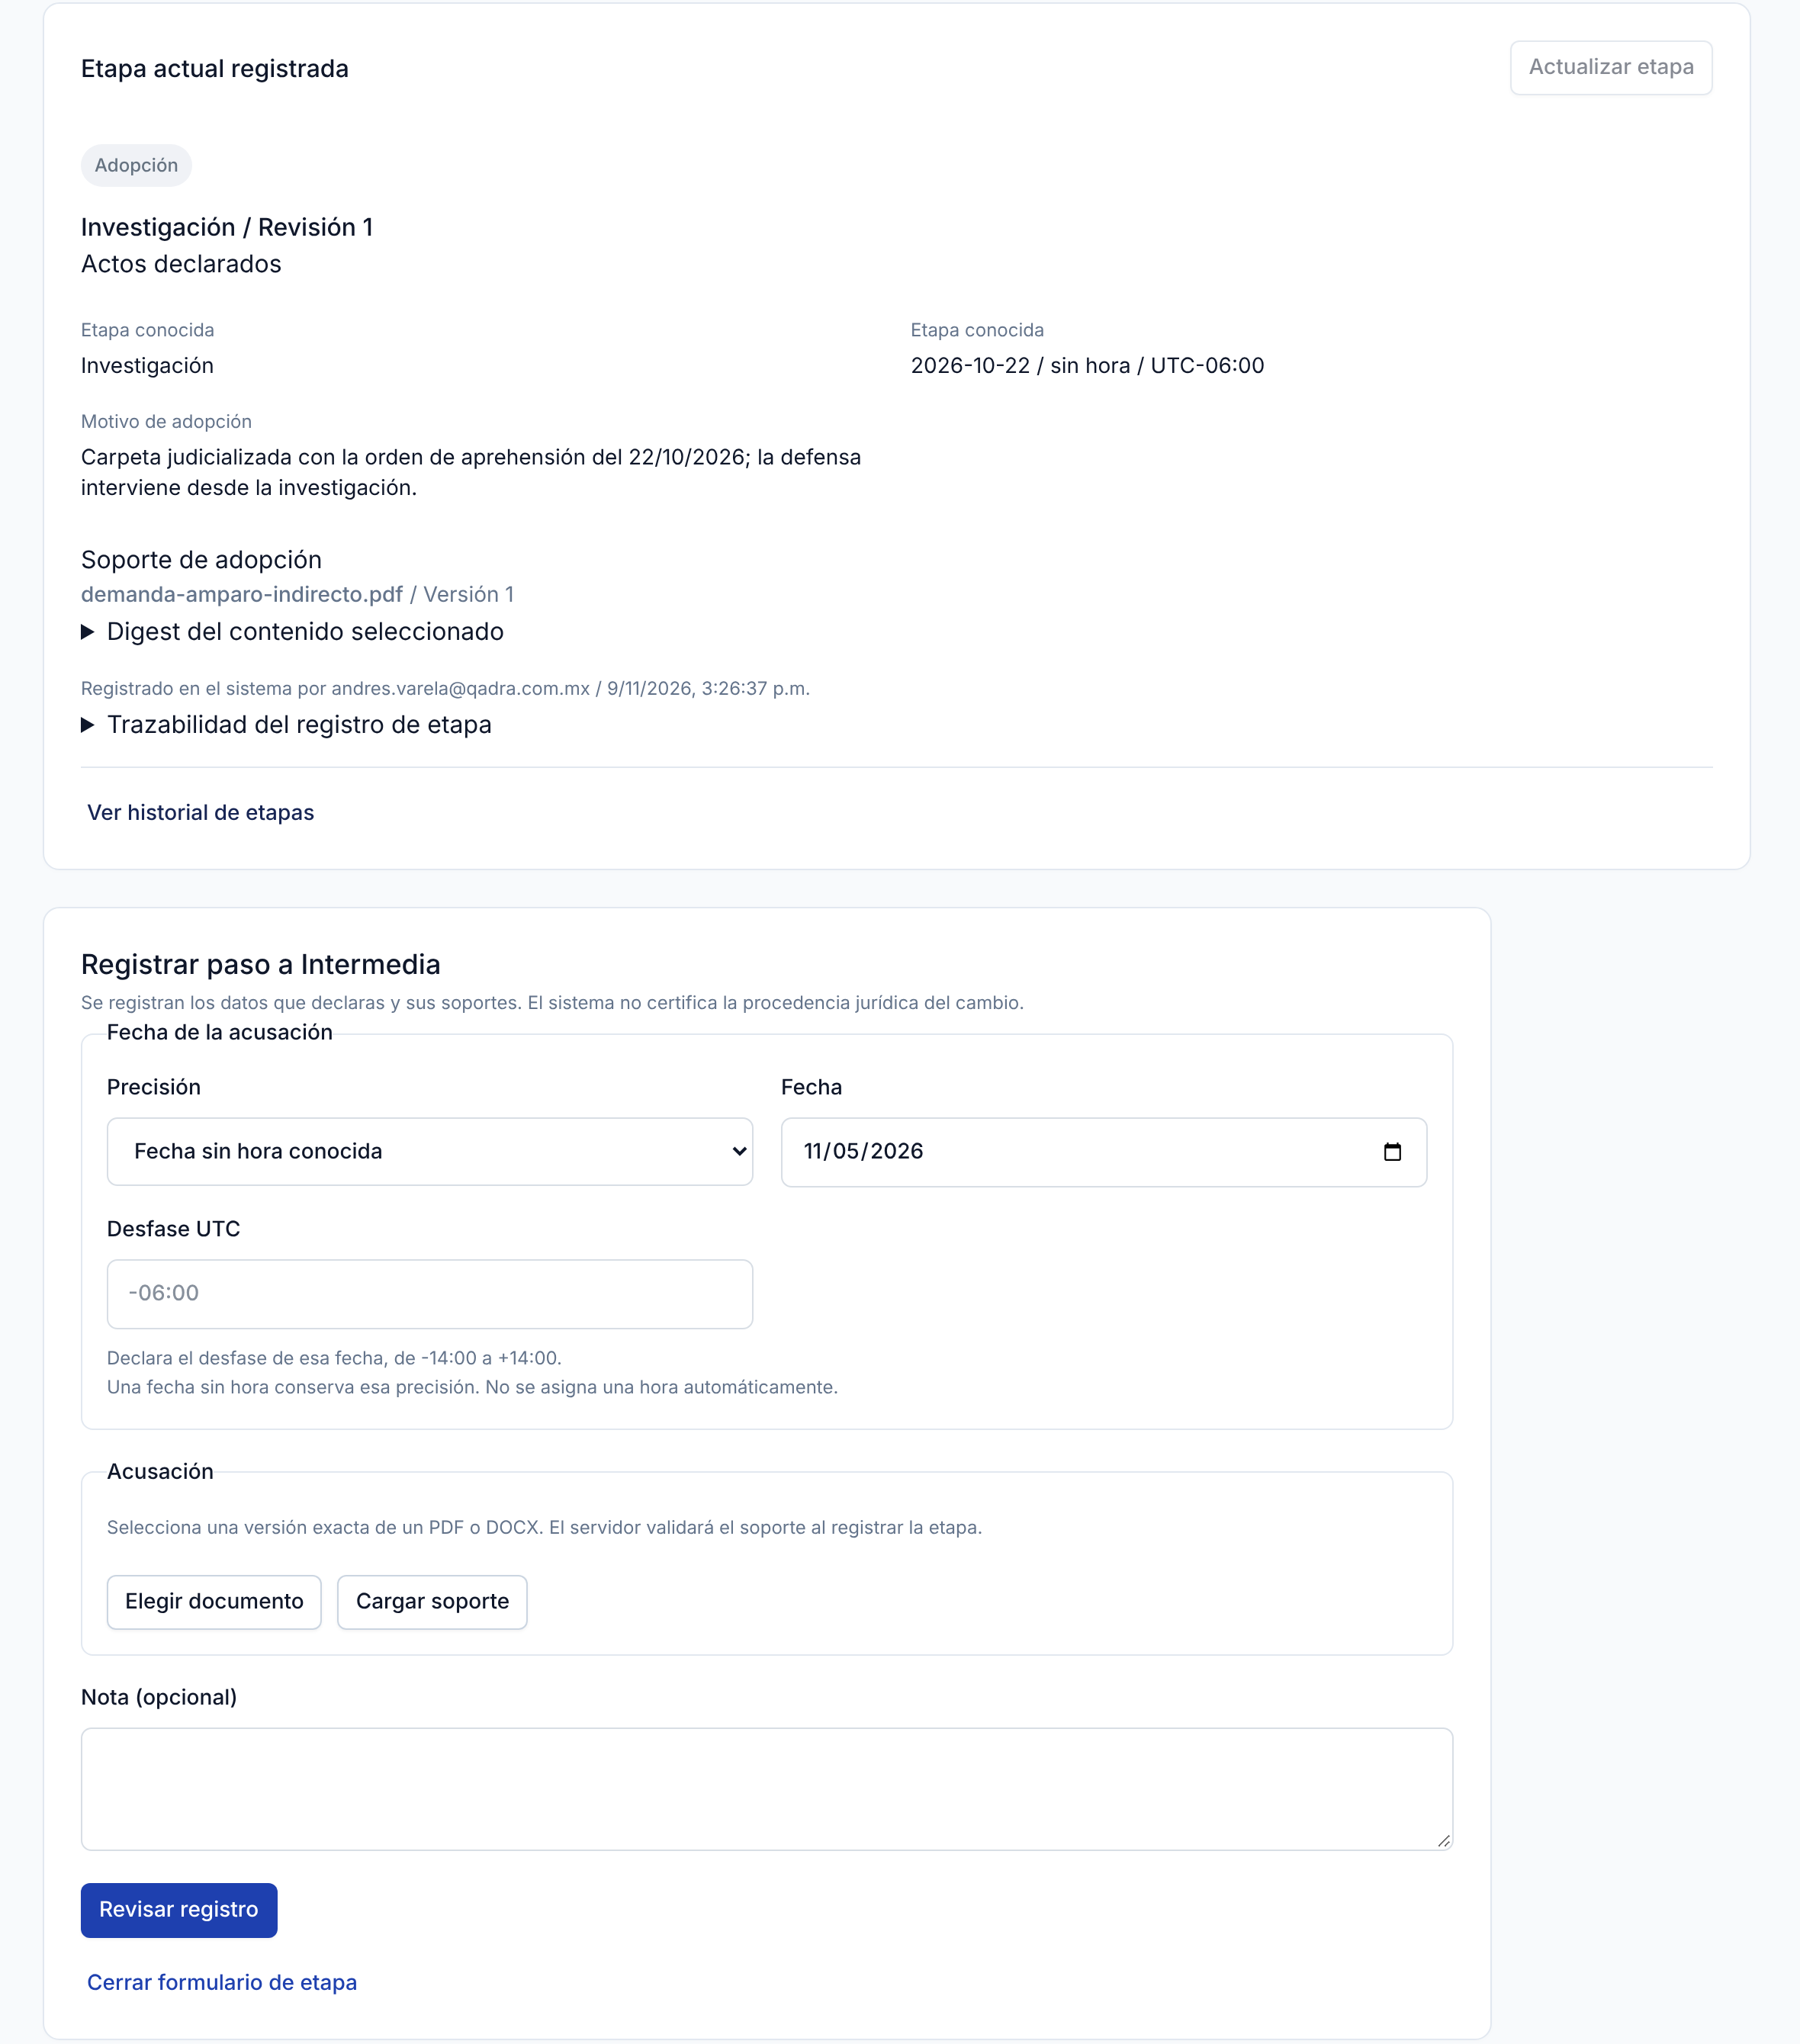
\includegraphics[width=0.9\textwidth,height=0.8\textheight,keepaspectratio]{capturas/A-28-etapas.png}
  \caption{Registro de un cambio de etapa.}
  \label{fig:manual-etapas}
\end{figure}

\resultado La pestaña muestra la nueva \textbf{Etapa actual registrada}.

\nota{Las etapas solo avanzan: Investigación, Intermedia y Juicio. Si la
ficha no está completa aparece \enquote{Completa la ficha penal para
registrar una etapa.} con el botón \textbf{Ir al resumen}.}

% ---------------------------------------------------------------------
\section{Audiencias}\label{sec:audiencias}

\paraque Programa audiencias, registra lo que ocurrió en ellas y conserva
cada cambio. También reúne las audiencias cautelares.

\disponible Administrador y Litigante (registran); Asistente legal
(consulta). Requiere la ficha penal completa y una etapa registrada.

\begin{table}[H]
  \centering
  \caption{Acciones en Audiencias.}\label{tab:acciones-audiencias}
  \begin{tabularx}{\textwidth}{L{4.6cm} Y}
    \toprule
    \textbf{Botón} & \textbf{Qué hace} \\
    \midrule
    \textbf{Programar audiencia}         & Registra una audiencia nueva. \\
    \textbf{Corregir o reprogramar}      & Cambia fecha, sede u otros datos, con su motivo. \\
    \textbf{Cancelar audiencia}          & Cancela la audiencia, con su motivo. \\
    \textbf{Ver sesiones y resultados}   & Registra qué ocurrió: \textbf{Registrar sesión o acto}, \textbf{Registrar continuación}, \textbf{Rectificar registro} o \textbf{Retirar registro}. \\
    \textbf{Registrar resultado y plazo} & Guarda el resultado y el plazo que genera en un solo paso. \\
    \textbf{Programar audiencia cautelar}& Convoca una audiencia de imposición o revisión de medidas cautelares. \\
    \textbf{Ver historial de audiencias} & Muestra todas las versiones de la audiencia. \\
    \bottomrule
  \end{tabularx}
\end{table}

\pasos\ Programar una audiencia:
\begin{enumerate}
  \item En la pestaña \textbf{Audiencias}, haga clic en
        \textbf{Programar audiencia}.
  \item Elija el \textbf{Tipo de audiencia}: Inicial, Intermedia, Debate de
        juicio o Individualización de sanciones y reparación del daño. Debe
        corresponder a la etapa registrada.
  \item Elija la \textbf{Modalidad} (\textbf{Presencial} o
        \textbf{Videoconferencia}), la fecha, la hora y la
        \textbf{Sede o conexión}.
  \item Agregue los participantes previstos: haga clic en
        \textbf{Elegir participante}, abra la ficha con
        \textbf{Consultar ficha: }\emph{nombre} y confirme con
        \textbf{Vincular esta revisión}. Repita para cada persona; la lista
        aparece en \textbf{Participantes previstos}.
  \item Haga clic en \textbf{Revisar registro} y después en
        \textbf{Confirmar registro}.
\end{enumerate}

\begin{figure}[H]
  \centering
  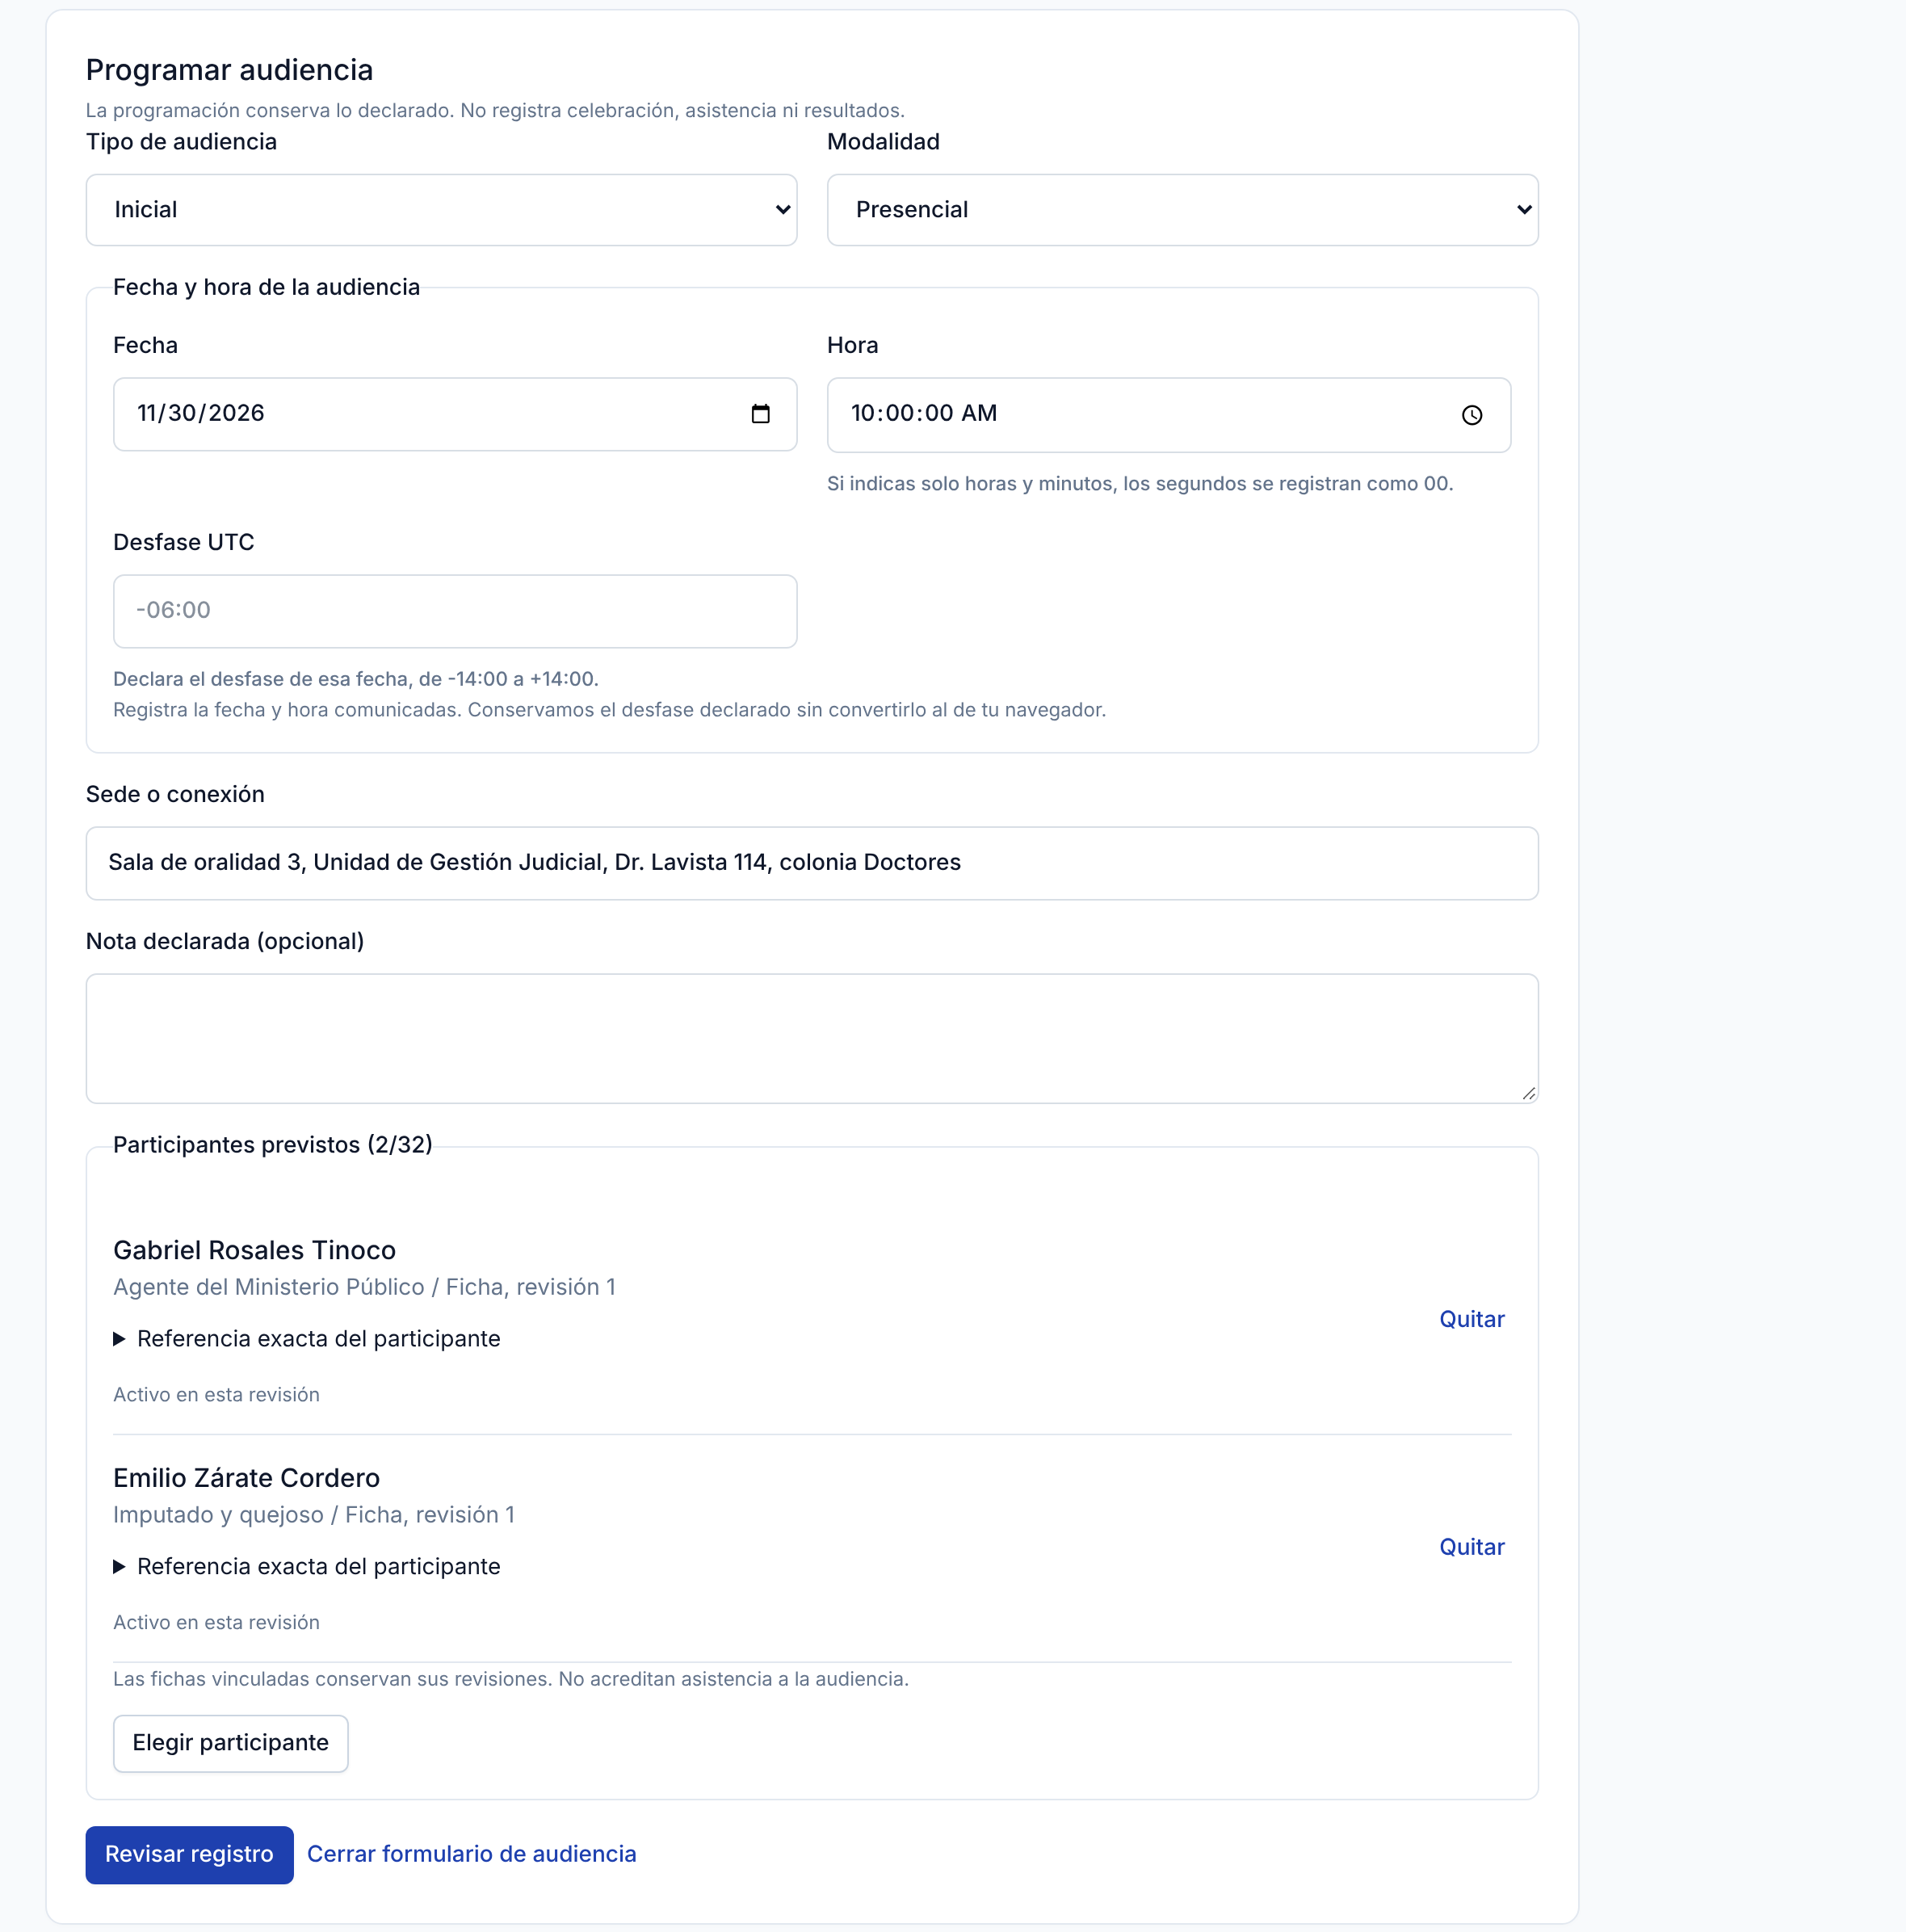
\includegraphics[width=0.9\textwidth,height=0.8\textheight,keepaspectratio]{capturas/A-29-programar-audiencia.png}
  \caption{Programación de una audiencia.}
  \label{fig:manual-programar-audiencia}
\end{figure}

\resultado La audiencia aparece como \textbf{Programada} en la lista y en la
\textbf{Agenda}.

\nota{Programar no acredita que la audiencia se celebró; regístrelo después
en \textbf{Ver sesiones y resultados}. Retirar un resultado conserva su
historia y no anula el acto informado.}

% ---------------------------------------------------------------------
\section{Medidas cautelares}\label{sec:medidas-cautelares}

\paraque Registra las decisiones sobre medidas cautelares (imposición,
modificación, revocación, sustitución) y lleva el registro de cada medida.

\disponible Administrador y Litigante (registran); Asistente legal
(consulta).

\begin{table}[H]
  \centering
  \caption{Acciones en Medidas cautelares.}\label{tab:acciones-medidas}
  \begin{tabularx}{\textwidth}{L{4.8cm} Y}
    \toprule
    \textbf{Botón} & \textbf{Qué hace} \\
    \midrule
    \textbf{Registrar decisión cautelar}   & Registra una decisión y sus efectos sobre las medidas. \\
    \textbf{Consultar decisión cautelar}   & Muestra la decisión con sus fuentes. \\
    \textbf{Consultar medida}              & Muestra el registro de una medida y su historia. \\
    \textbf{Rectificar registro}           & Corrige el registro de una medida, con su motivo. \\
    \textbf{Marcar registro por error}     & Señala un registro capturado por error. \\
    \bottomrule
  \end{tabularx}
\end{table}

\pasos\ Registrar una decisión cautelar:
\begin{enumerate}
  \item En la pestaña \textbf{Medidas cautelares}, haga clic en
        \textbf{Registrar decisión cautelar}.
  \item Indique la \textbf{Autoridad}, la \textbf{Precisión de decisión}
        y la fecha, la \textbf{Justificación} y el \textbf{Resultado}
        (\textbf{Cambios en medidas} o \textbf{Sin cambio en medidas}).
  \item Con \textbf{Cambios en medidas}, el formulario muestra el
        \textbf{Efecto 1}: elija la \textbf{Acción de medida}
        (\textbf{Imponer}, \textbf{Confirmar}, \textbf{Modificar},
        \textbf{Revocar}, \textbf{Cesar} o \textbf{Sustituir}), la persona
        (\textbf{Elegir sujeto}), la \textbf{Clase de medida}, las
        \textbf{Condiciones} y la vigencia. Para otro efecto, haga clic en
        \textbf{Agregar efecto}.
  \item Indique si la decisión viene de una audiencia (inicial o cautelar)
        o es independiente.
  \item Haga clic en \textbf{Revisar decisión} y después en
        \textbf{Confirmar decisión}.
\end{enumerate}

\begin{figure}[H]
  \centering
  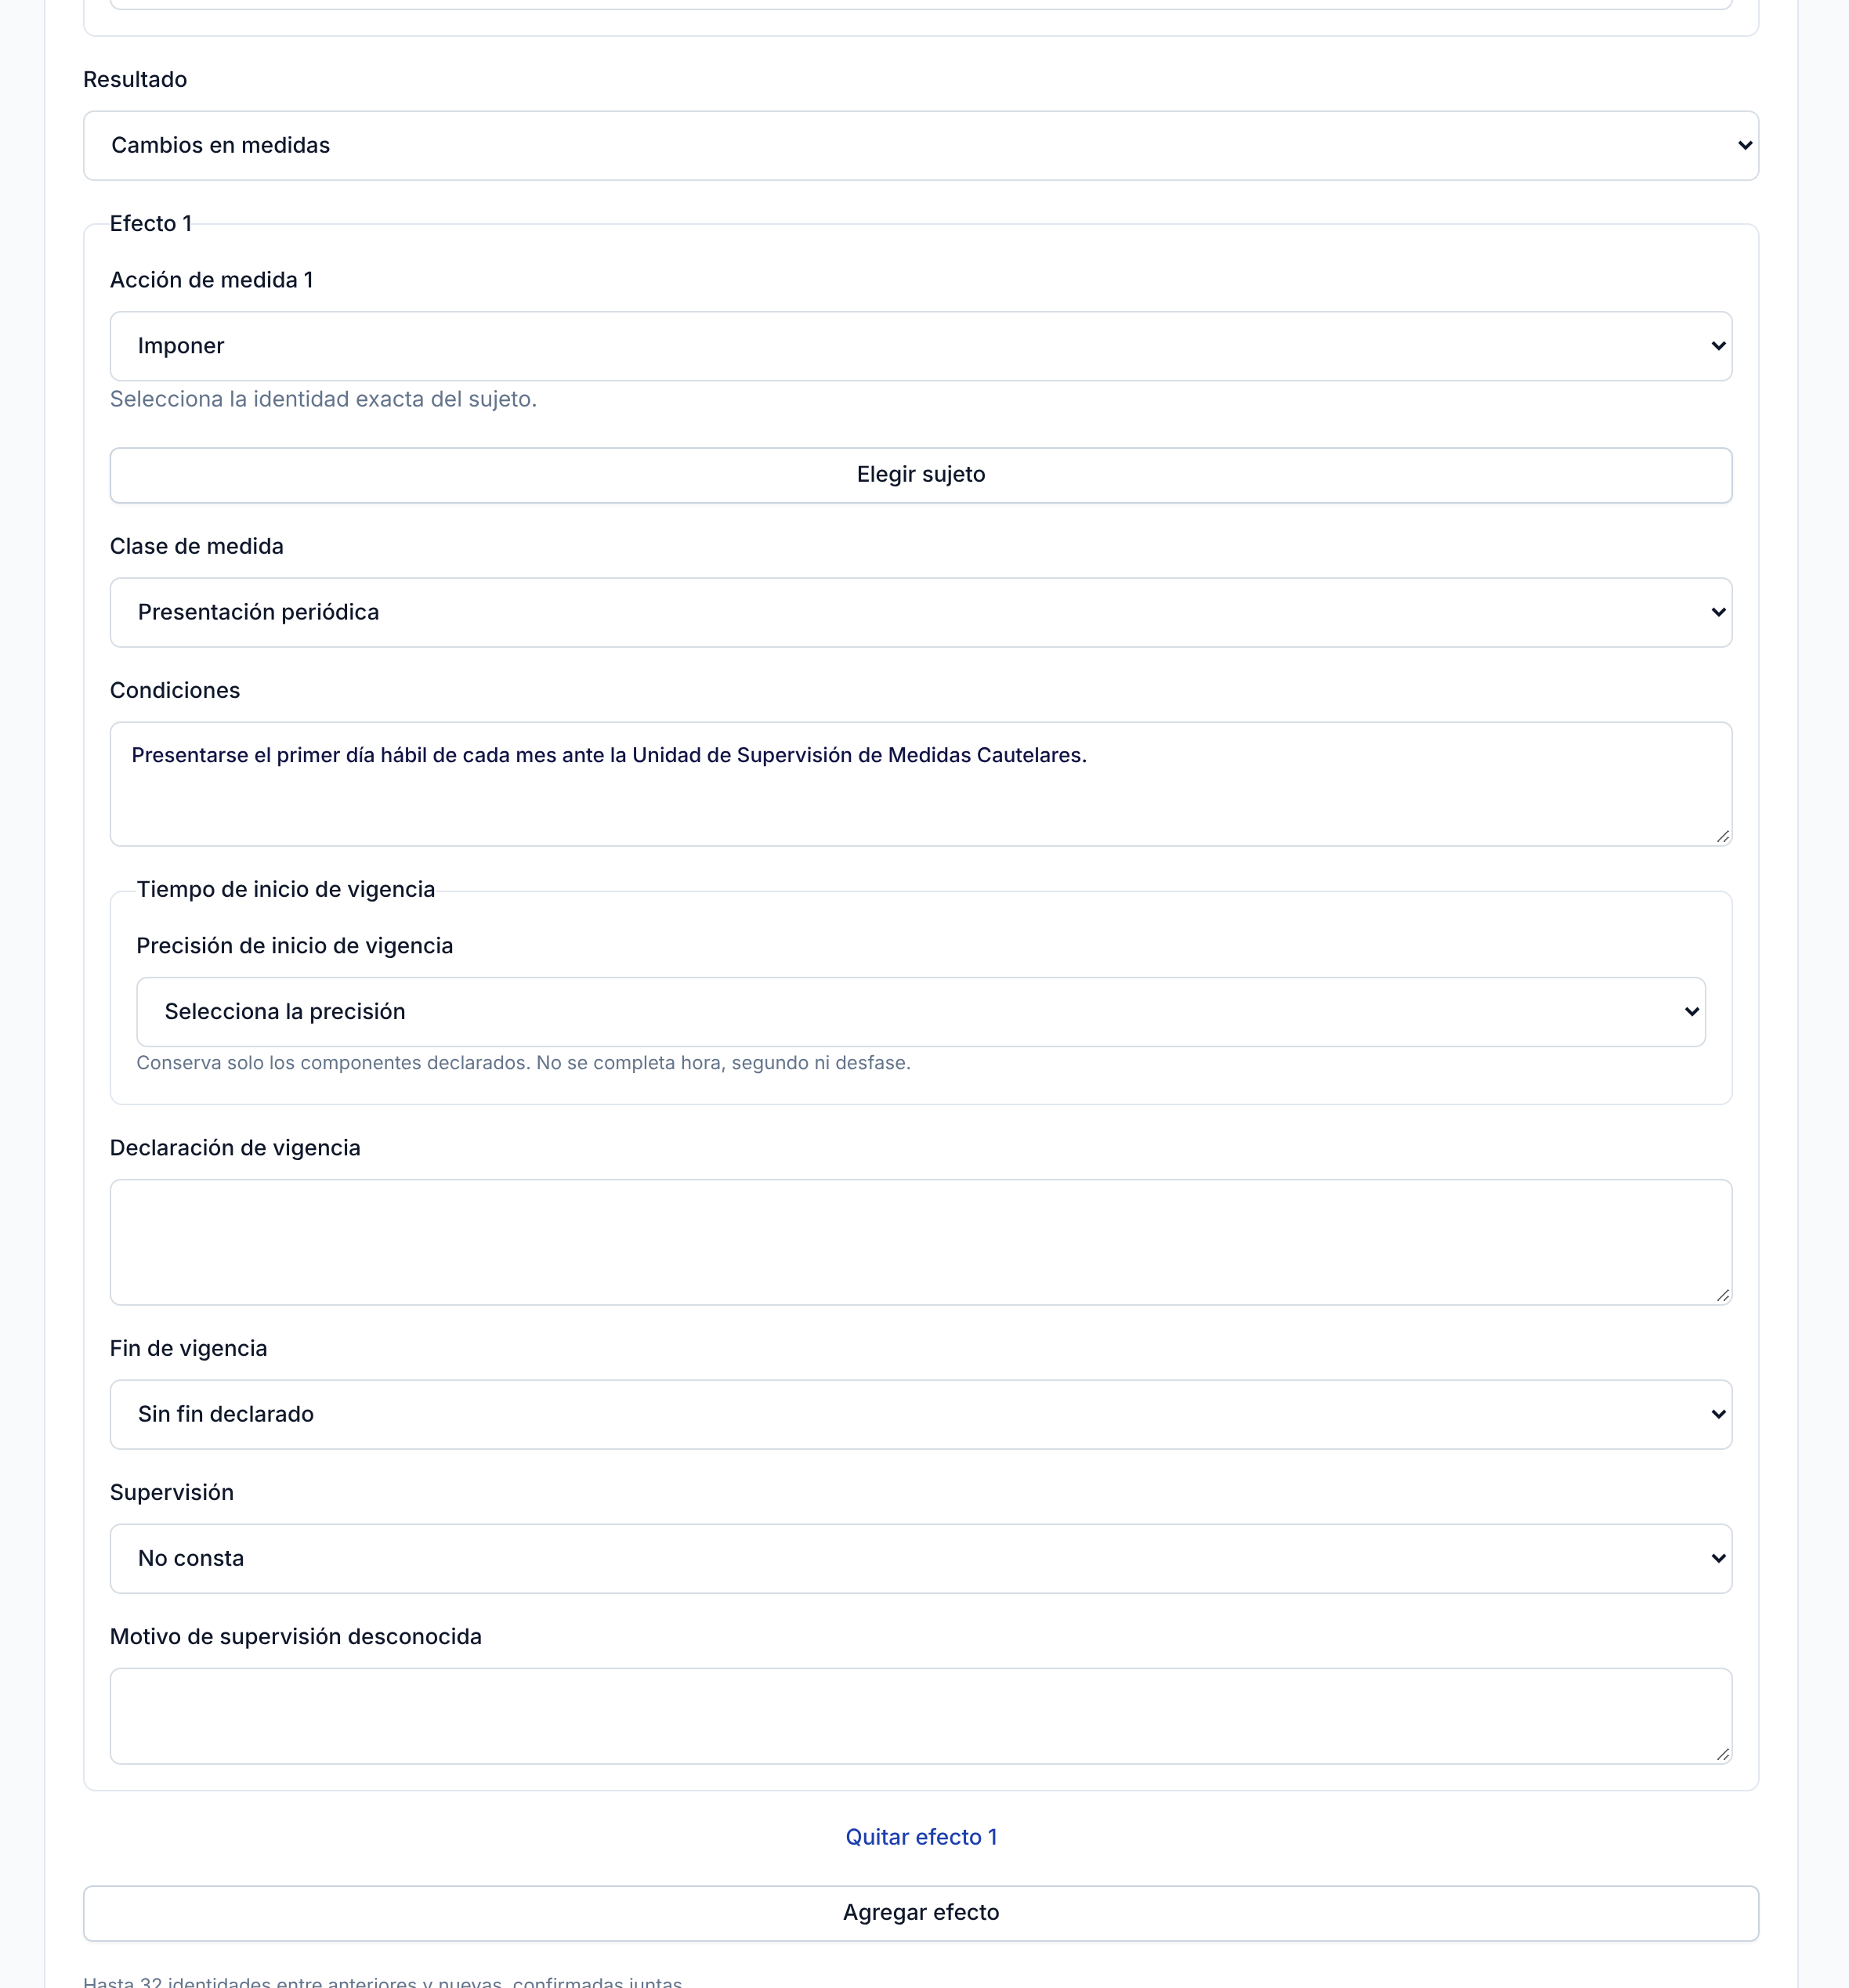
\includegraphics[width=0.9\textwidth,height=0.8\textheight,keepaspectratio]{capturas/A-30-decision-cautelar.png}
  \caption{Registro de una decisión cautelar.}
  \label{fig:manual-decision-cautelar}
\end{figure}

\resultado La decisión y las medidas afectadas aparecen en la pestaña.

\nota{Las audiencias cautelares se programan desde la pestaña
\textbf{Audiencias} (\cref{sec:audiencias}). El estado del expediente no
determina la vigencia jurídica de una medida.}

% ---------------------------------------------------------------------
\section{Resoluciones y notificaciones}\label{sec:resoluciones}

\paraque Registra las resoluciones del expediente y, dentro de cada una,
sus notificaciones.

\disponible Administrador y Litigante (registran); Asistente legal
(consulta).

\begin{table}[H]
  \centering
  \caption{Acciones en Resoluciones.}\label{tab:acciones-resoluciones}
  \begin{tabularx}{\textwidth}{L{4.8cm} Y}
    \toprule
    \textbf{Botón} & \textbf{Qué hace} \\
    \midrule
    \textbf{Registrar resolución}          & Registra un auto, una sentencia u otra resolución. \\
    \textbf{Corregir resolución} / \textbf{Retirar resolución}
                                           & Corrige o retira el registro; retirar no anula el acto. \\
    \textbf{Ver notificaciones}            & Abre las notificaciones de esa resolución. \\
    \textbf{Registrar notificación}        & Registra cómo y a quién se notificó. \\
    \textbf{Ver historial de resolución}   & Muestra todas las versiones del registro. \\
    \bottomrule
  \end{tabularx}
\end{table}

\pasos\ Registrar una resolución y su notificación:
\begin{enumerate}
  \item En la pestaña \textbf{Resoluciones}, haga clic en
        \textbf{Registrar resolución}.
  \item Elija la \textbf{Clase de resolución} (\textbf{Auto u orden},
        \textbf{Sentencia} u \textbf{Otra clase}), el \textbf{Emisor}, la
        fecha de emisión y el resumen.
  \item Haga clic en \textbf{Preparar registro} y después en
        \textbf{Confirmar registro}.
  \item En la resolución registrada, haga clic en \textbf{Ver notificaciones}
        y luego en \textbf{Registrar notificación}.
  \item Elija el \textbf{Carácter de notificación}, el
        \textbf{Medio de notificación}, el \textbf{Contexto de notificación}
        y el \textbf{Resultado declarado}. Confirme igual que en el paso 3.
\end{enumerate}

\begin{figure}[H]
  \centering
  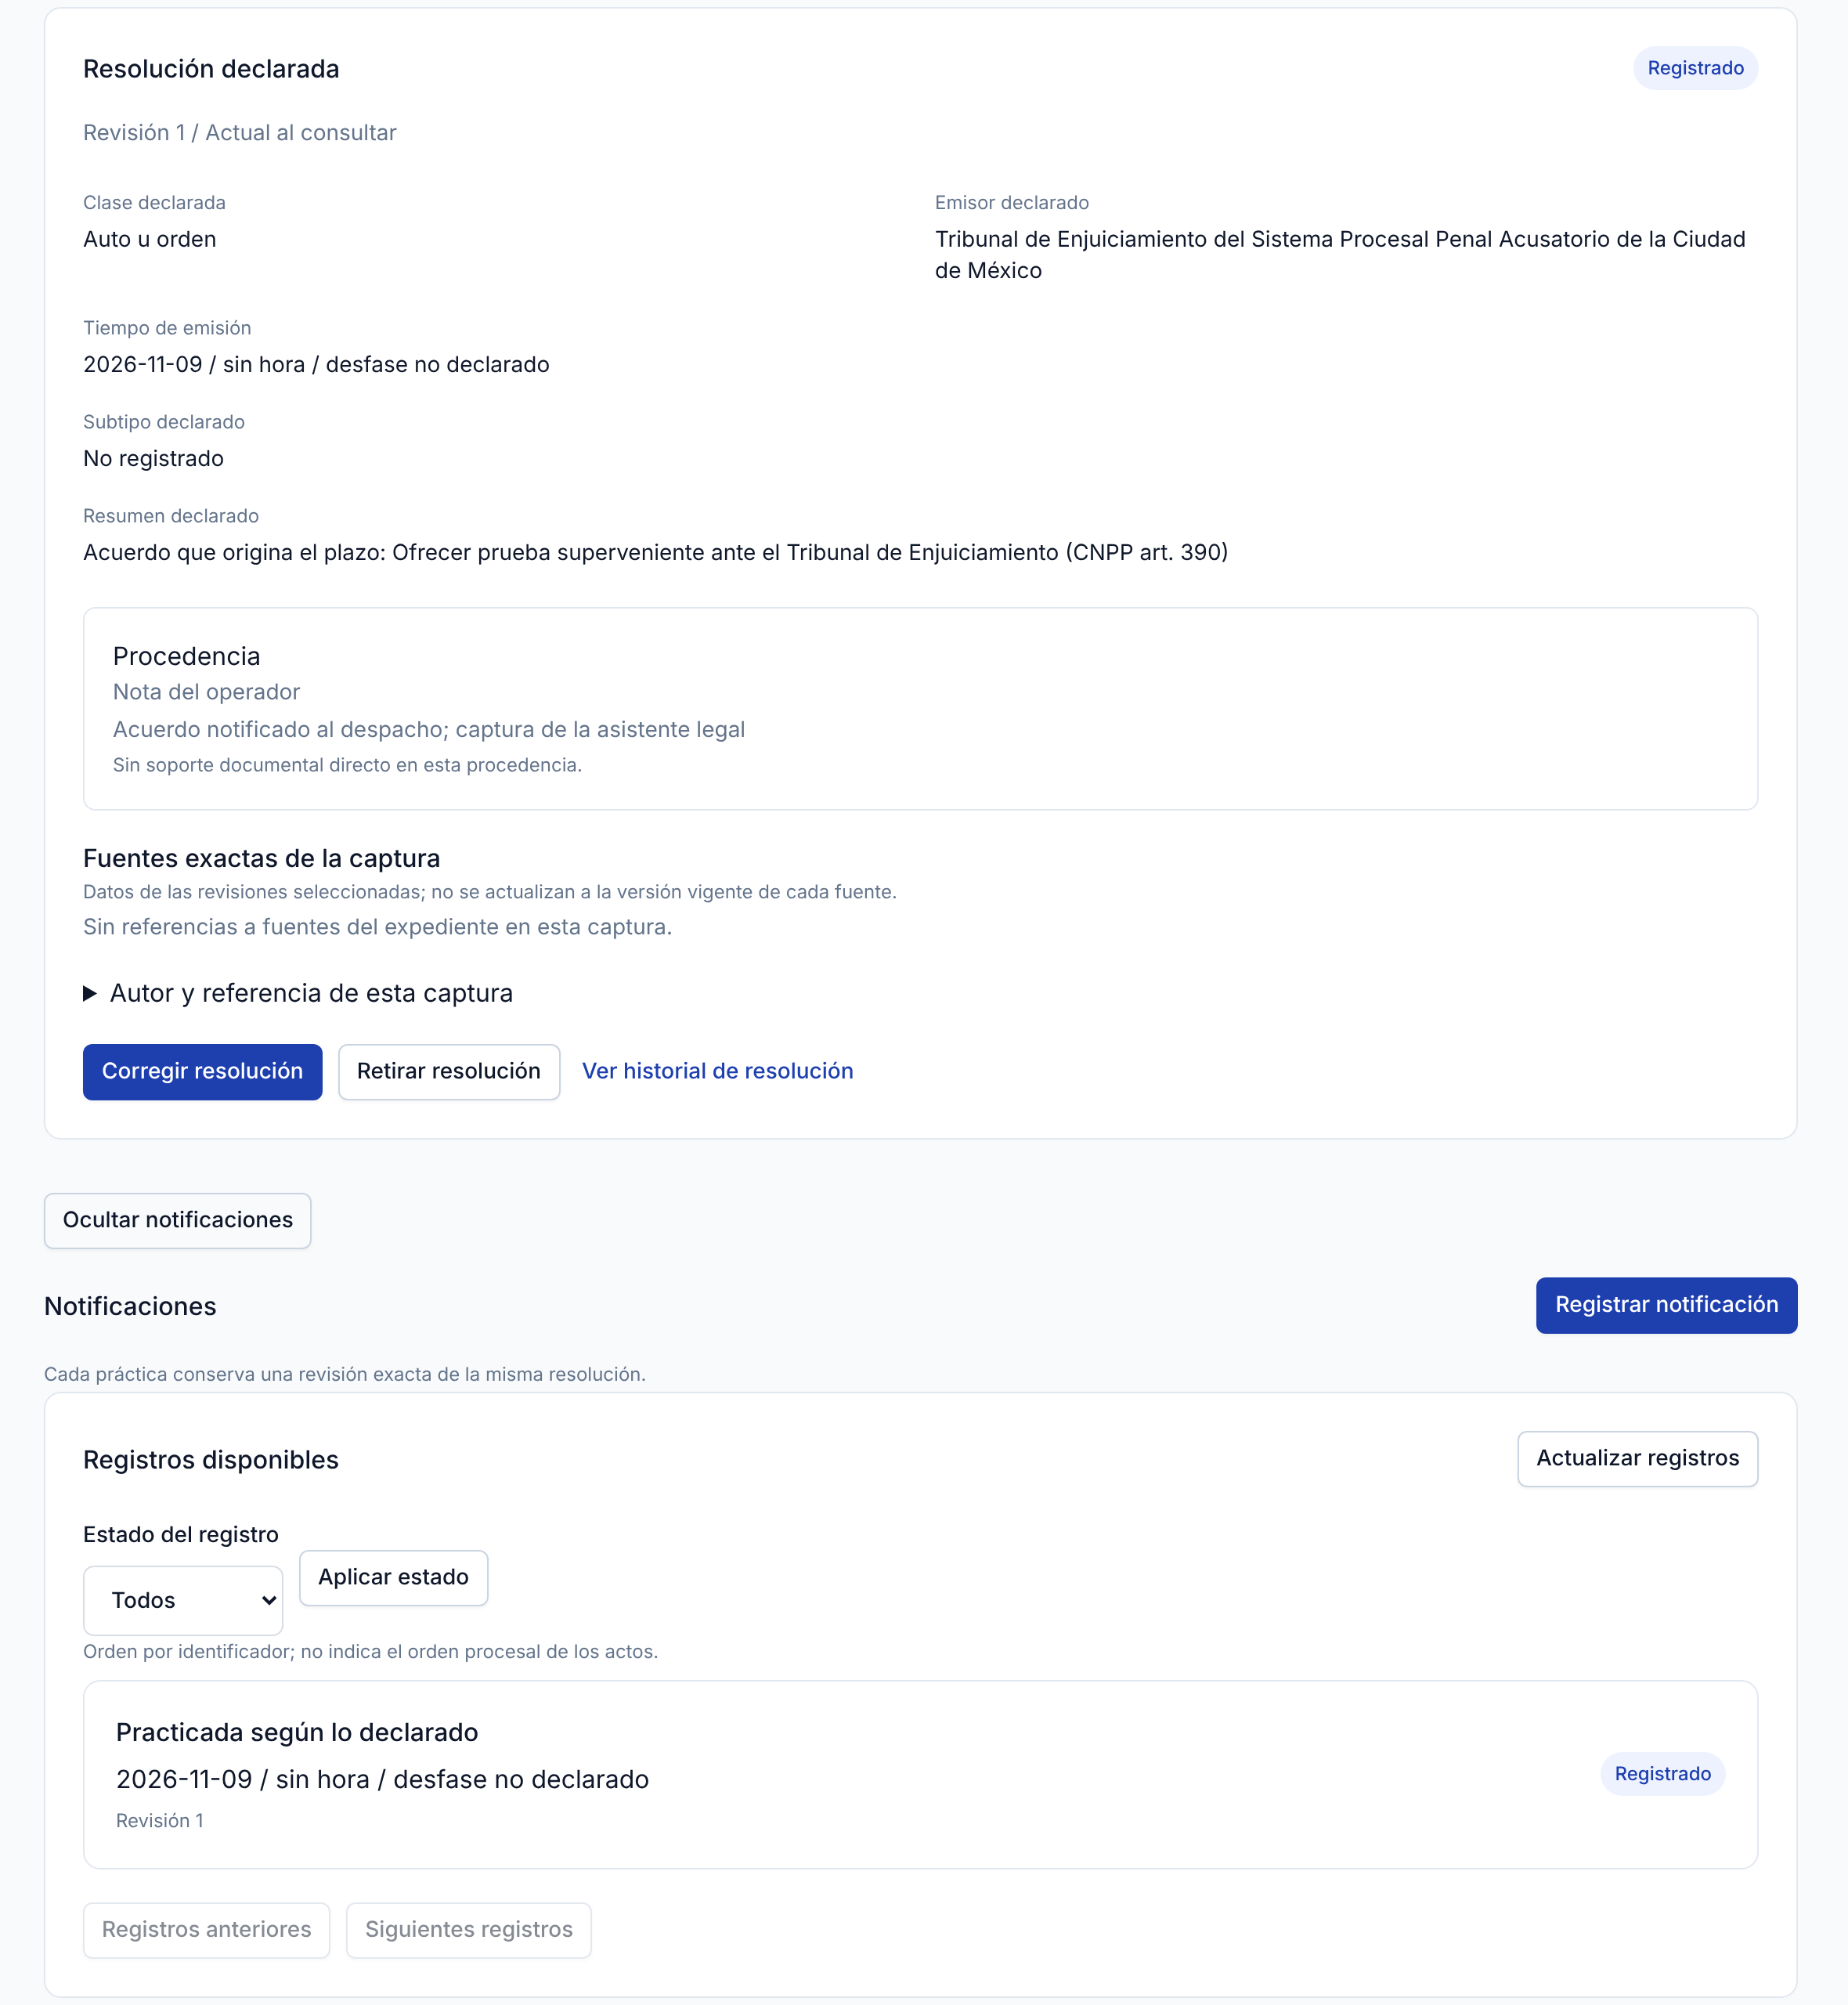
\includegraphics[width=0.9\textwidth,height=0.8\textheight,keepaspectratio]{capturas/A-31-resoluciones.png}
  \caption{Resoluciones y notificaciones.}
  \label{fig:manual-resoluciones}
\end{figure}

\resultado Qadra muestra \textbf{Registro guardado.} y la resolución aparece
en \textbf{Registros disponibles} con su notificación.

% ---------------------------------------------------------------------
\section{Recursos}\label{sec:recursos}

\paraque Registra recursos de revocación y apelación, sus actos y su
relación con audiencias y plazos.

\disponible Administrador y Litigante (registran); Asistente legal
(consulta).

\begin{table}[H]
  \centering
  \caption{Acciones en Recursos.}\label{tab:acciones-recursos}
  \begin{tabularx}{\textwidth}{L{4.8cm} Y}
    \toprule
    \textbf{Botón} & \textbf{Qué hace} \\
    \midrule
    \textbf{Registrar recurso}             & Registra una revocación o una apelación. \\
    \textbf{Registrar acto}                & Agrega interposición, admisión, inadmisibilidad, desistimiento o resolución. \\
    \textbf{Corregir recurso}              & Corrige los datos del recurso. \\
    \textbf{Archivar recurso} / \textbf{Reactivar recurso}
                                           & Ordena la lista; no declara desistimiento. \\
    \textbf{Vincular actividad}            & Relaciona una audiencia o un plazo existente. \\
    \textbf{Crear plazo}                   & Crea un plazo ya vinculado al recurso. \\
    \textbf{Crear audiencia de recurso}    & Programa una audiencia ya vinculada al recurso. \\
    \bottomrule
  \end{tabularx}
\end{table}

\pasos\ Registrar un recurso:
\begin{enumerate}
  \item En la pestaña \textbf{Recursos}, haga clic en
        \textbf{Registrar recurso}.
  \item Elija el \textbf{Tipo de recurso} (\textbf{Revocación} o
        \textbf{Apelación}) y llene los datos: parte impugnada, personas
        recurrentes, motivos, \textbf{Modalidad del recurso}, autoridades y
        \textbf{Referencia de la resolución}.
  \item Haga clic en \textbf{Preparar registro} y después en
        \textbf{Confirmar registro}.
\end{enumerate}

\begin{figure}[H]
  \centering
  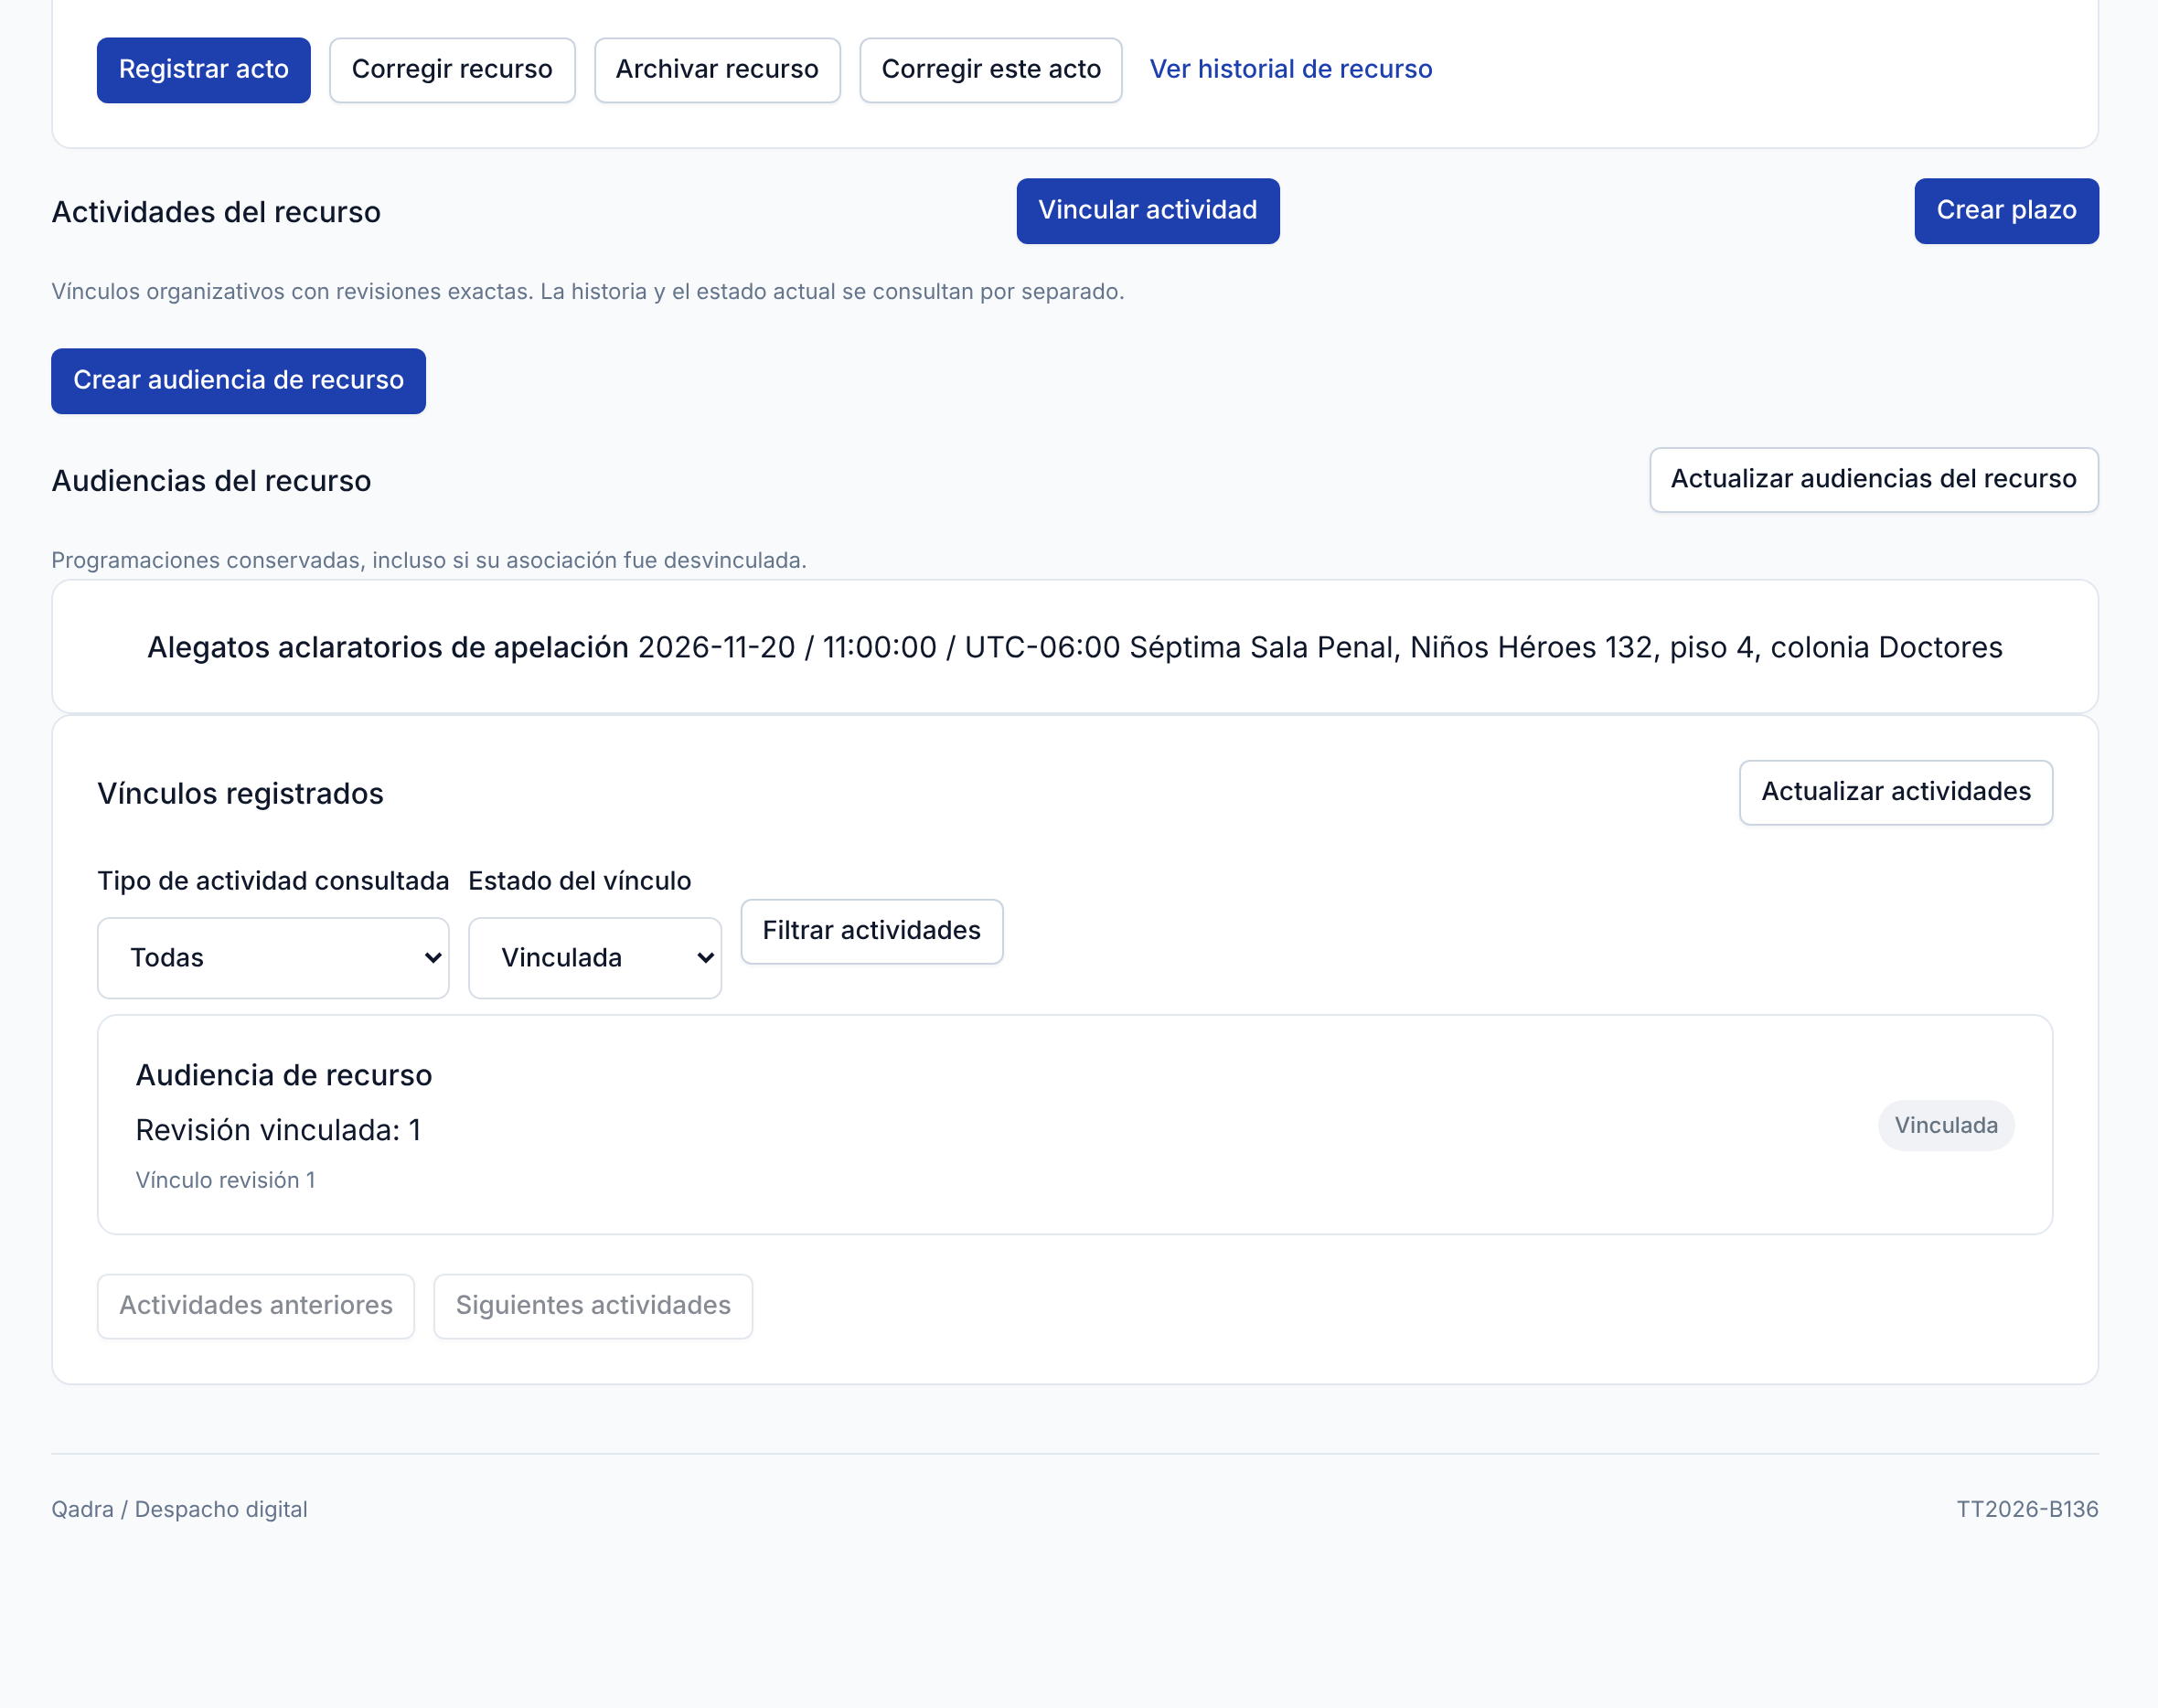
\includegraphics[width=0.9\textwidth,height=0.8\textheight,keepaspectratio]{capturas/A-32-recursos.png}
  \caption{Recursos procesales.}
  \label{fig:manual-recursos}
\end{figure}

\resultado El recurso aparece en \textbf{Recursos del expediente}. Desde ahí
puede registrar sus actos y vincular actividades.

% ---------------------------------------------------------------------
\section{Plazos}\label{sec:plazos}

\paraque Calcula el vencimiento de un plazo a partir de su fuente, su regla
y el calendario judicial, y registra si ya se atendió.

\disponible Administrador y Litigante (registran); Asistente legal
(consulta).

\begin{table}[H]
  \centering
  \caption{Acciones en Plazos.}\label{tab:acciones-plazos}
  \begin{tabularx}{\textwidth}{L{4.4cm} Y}
    \toprule
    \textbf{Botón} & \textbf{Qué hace} \\
    \midrule
    \textbf{Registrar plazo}          & Crea un plazo y calcula su vencimiento. \\
    \textbf{Corregir plazo}           & Corrige fuente, regla, calendario o responsable. \\
    \textbf{Revisar seguimiento}      & Aparece cuando un cambio en la fuente o la regla requiere su revisión. \\
    \textbf{Declarar atención}        & Registra que el plazo ya se atendió. \\
    \textbf{Retirar plazo}            & Retira el plazo; su cálculo queda en el historial. \\
    \textbf{Ver historial de plazo}   & Muestra cada cálculo y quién lo hizo. \\
    \bottomrule
  \end{tabularx}
\end{table}

\pasos\ Registrar un plazo:
\begin{enumerate}
  \item En la pestaña \textbf{Plazos}, haga clic en \textbf{Registrar plazo}.
  \item Escriba el \textbf{Título del plazo}.
  \item En \textbf{Regla aplicable}, haga clic en
        \textbf{Elegir perfil exacto}, elija el perfil, abra su revisión con
        \textbf{Consultar perfil revisión} y confirme con
        \textbf{Usar este perfil exacto}. En \textbf{Cuando cambie el
        perfil} elija \textbf{Conservar esta revisión} o
        \textbf{Seguir cambios y solicitar revisión}.
  \item En \textbf{Responsable}, haga clic en
        \textbf{Elegir responsable} y elija a la persona que lo atenderá.
  \item En \textbf{Fuente exacta del inicio}, elija el
        \textbf{Tipo de fuente} (\textbf{Resolución},
        \textbf{Notificación} o \textbf{Resultado de audiencia}), haga clic
        en \textbf{Elegir fuente exacta}, abra la revisión con
        \textbf{Consultar revisiones de la fuente} y vincúlela con
        \textbf{Vincular esta revisión}. Elija también cómo seguir los
        cambios de la fuente.
  \item En \textbf{Calendario}, haga clic en
        \textbf{Elegir calendario exacto} y elija su revisión con
        \textbf{Usar este calendario exacto}; para seguir sus cambios,
        elija \textbf{Seguir cambios del calendario}.
  \item Complete la \textbf{Declaración de aplicabilidad}, el
        \textbf{Localizador de aplicabilidad}, las preguntas sobre el
        ámbito del perfil, la incidencia sin resolver y cada condición del
        perfil.
  \item Haga clic en \textbf{Preparar plazo}. Revise el resultado en
        \textbf{Cálculo conservado en esta revisión} y los pasos en
        \textbf{Ver pasos del cómputo}.
  \item Marque \textbf{Revisé las declaraciones, fuentes, políticas y el
        resultado a guardar} y haga clic en \textbf{Confirmar plazo}. Si
        necesita cambiar algo, use \textbf{Volver al borrador}.
\end{enumerate}

\begin{figure}[H]
  \centering
  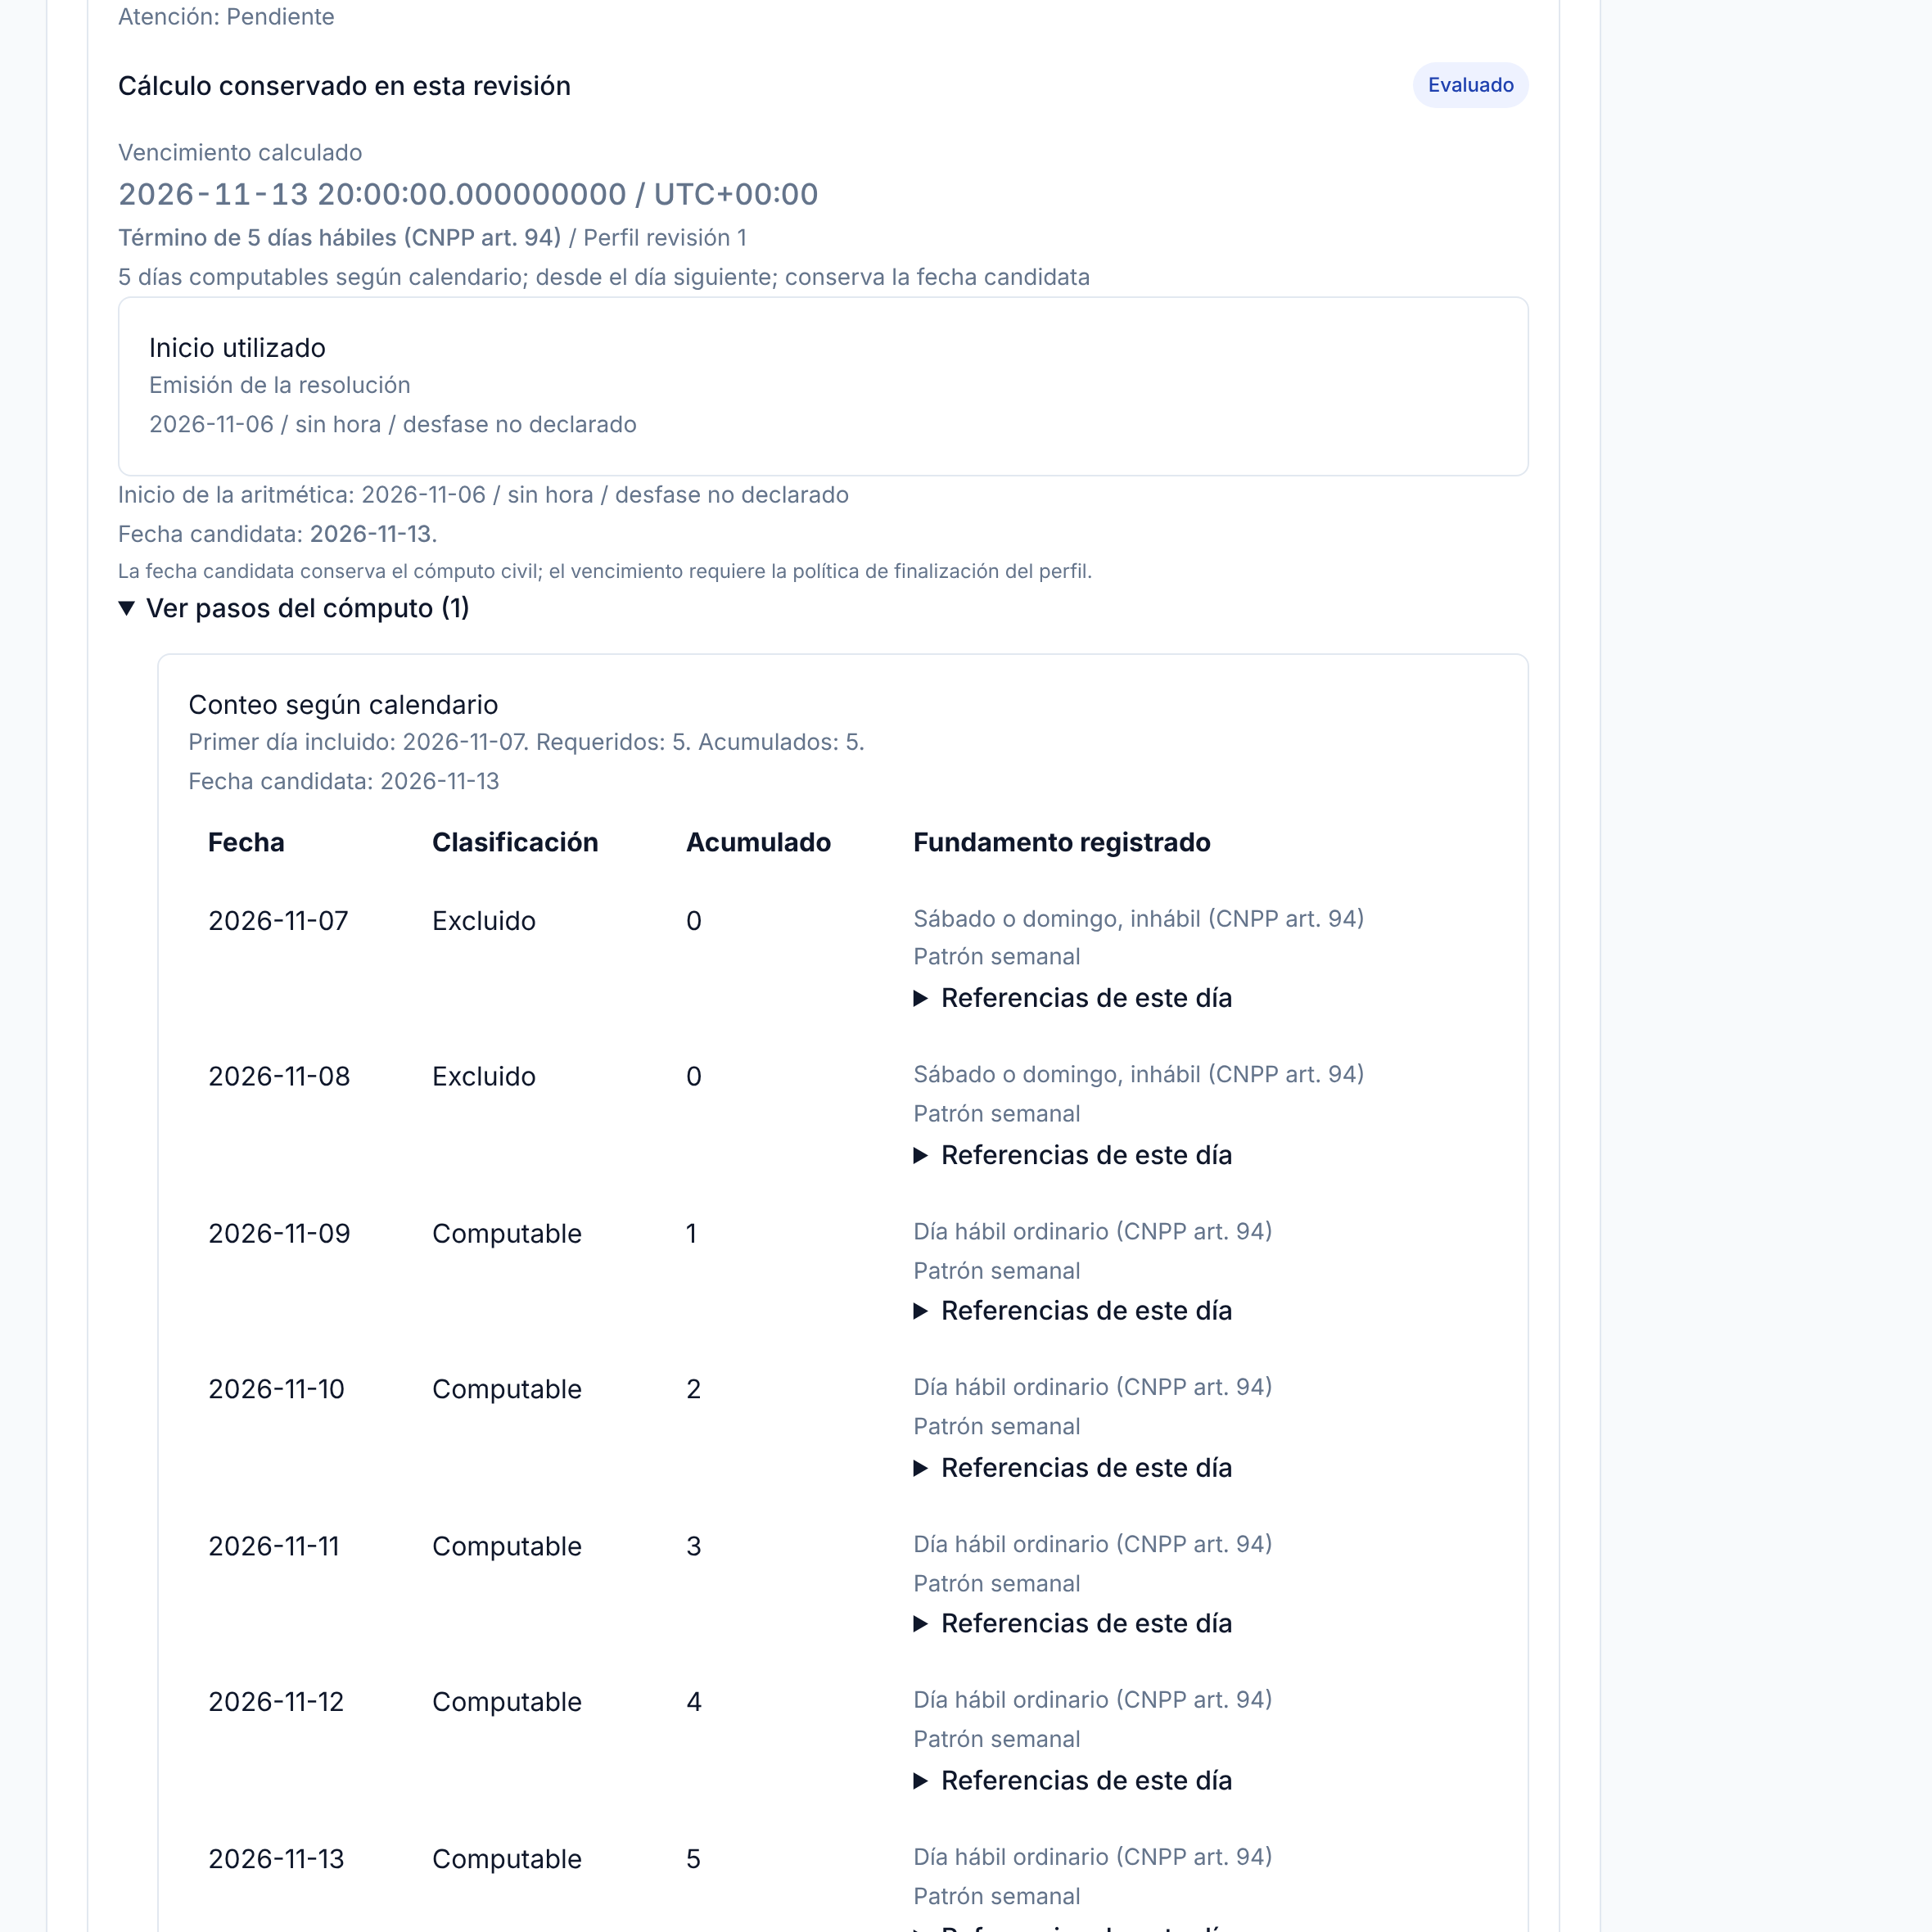
\includegraphics[width=0.9\textwidth,height=0.8\textheight,keepaspectratio]{capturas/A-33-registrar-plazo.png}
  \caption{Registro de un plazo.}
  \label{fig:manual-registrar-plazo}
\end{figure}

\resultado El plazo aparece en \textbf{Seguimiento de plazos} con su
\textbf{Vencimiento para seguimiento} y en la \textbf{Agenda}.

\begin{itemize}
  \item Si falta información, el plazo queda con \textbf{Cálculo bloqueado}:
        Qadra no inventa un vencimiento. Complete lo que falta con
        \textbf{Corregir plazo}.
  \item Elegir un responsable no le da acceso al expediente.
  \item Declarar atención o leer una alerta no acredita por sí solo una
        presentación válida.
\end{itemize}

\chapter{Agenda y Alertas}\label{cap:agenda-alertas}

% ---------------------------------------------------------------------
\section{Agenda}\label{sec:agenda}

\paraque Reúne en un calendario las audiencias y los vencimientos de plazos
de todos los expedientes a los que usted tiene acceso.

\disponible Administrador, Litigante y Asistente legal.

\pasos
\begin{enumerate}
  \item En el menú, haga clic en \textbf{Agenda}. Se abre la
        \textbf{Agenda del despacho} en la vista \textbf{Semana}.
  \item En \textbf{Vista de agenda}, elija \textbf{Día}, \textbf{Semana},
        \textbf{Mes} o \textbf{Rango personalizado}.
  \item Elija la \textbf{Fecha de referencia} (con su \textbf{Desfase de
        consulta}), o haga clic en un día del
        calendario que aparece junto a la lista; las flechas del calendario
        cambian el mes mostrado.
  \item En \textbf{Estado de audiencia} elija \textbf{Programadas},
        \textbf{Canceladas} o \textbf{Todas}. En \textbf{Tipo de actividad},
        elija qué mostrar:
        \textbf{Audiencias y plazos}, \textbf{Audiencias}, \textbf{Plazos},
        \textbf{Audiencias de recursos} o \textbf{Audiencias cautelares}.
  \item Haga clic en \textbf{Consultar Agenda}.
  \item Haga clic en una actividad de \textbf{Actividades en el periodo}
        para abrirla en su expediente.
\end{enumerate}

\begin{figure}[H]
  \centering
  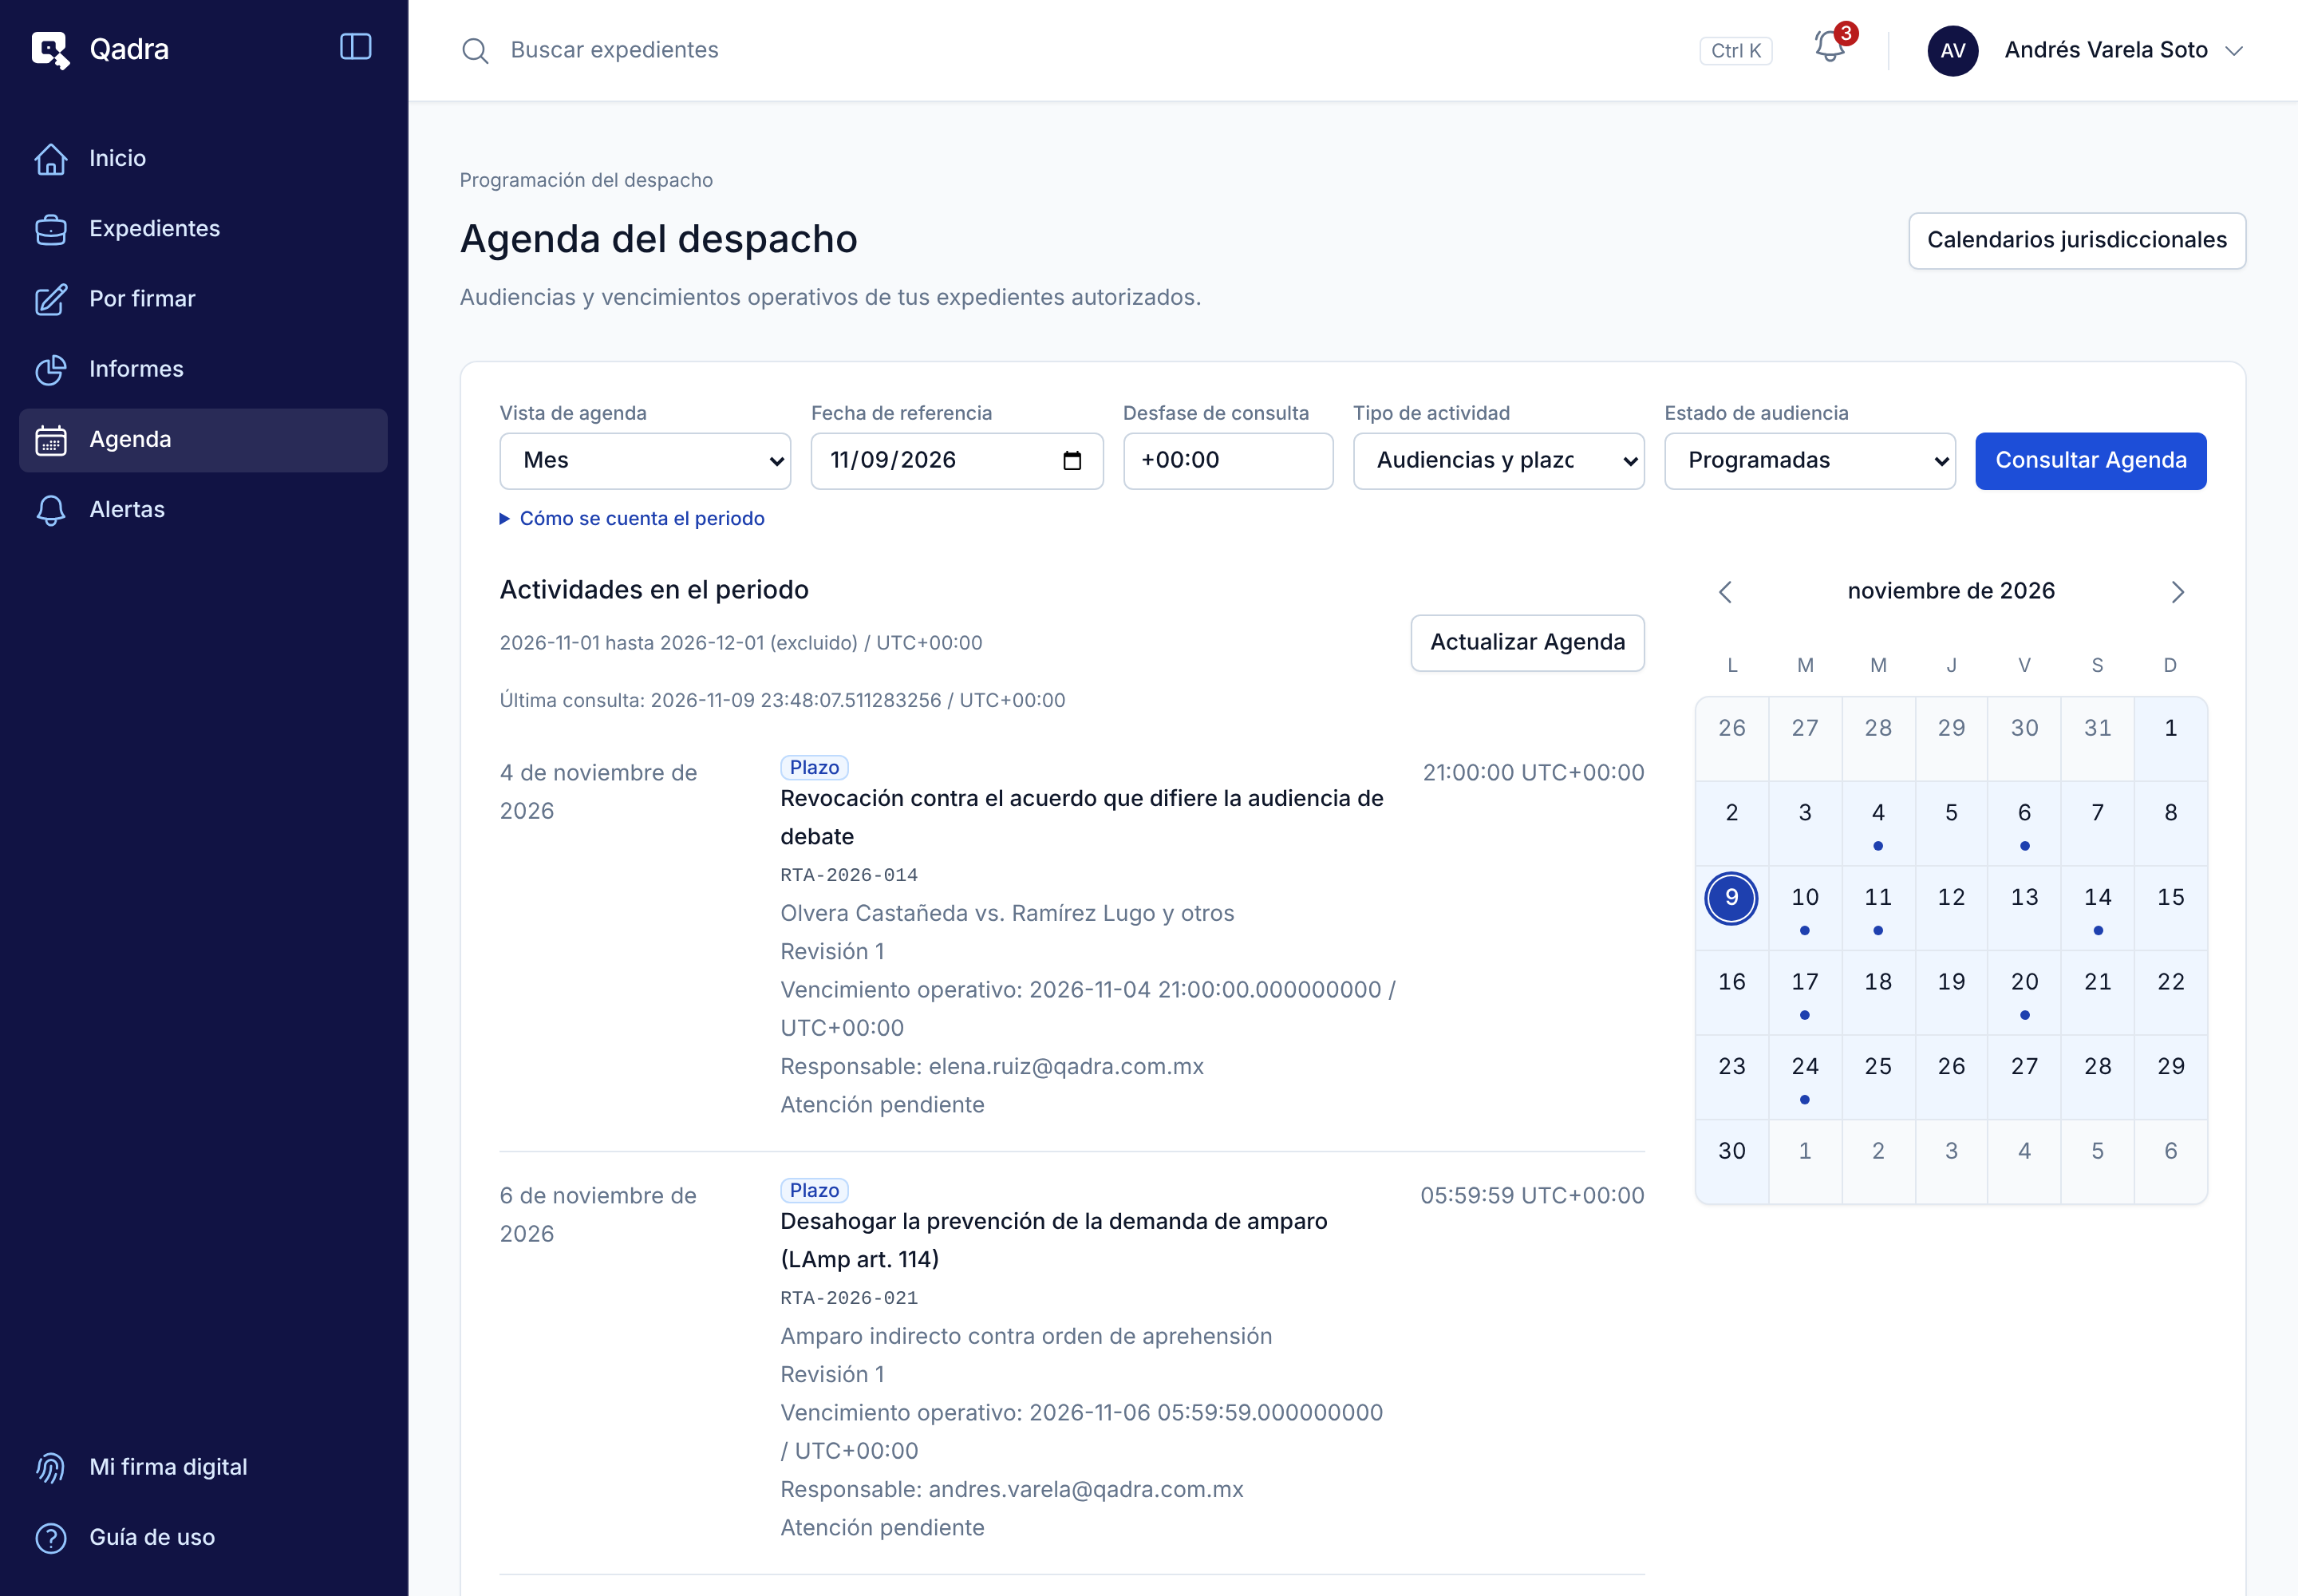
\includegraphics[width=0.9\textwidth,height=0.8\textheight,keepaspectratio]{capturas/A-34-agenda.png}
  \caption{Agenda del despacho.}
  \label{fig:manual-agenda}
\end{figure}

\resultado Ve sus audiencias y vencimientos del periodo, y abre cada uno en
un clic.

\begin{itemize}
  \item Si aparece \enquote{Consulta parcial: faltan actividades por
        consultar.}, haga clic en \textbf{Cargar más actividades}.
  \item Las actividades pueden cambiar entre consultas. Haga clic en
        \textbf{Actualizar Agenda} antes de tomar una decisión.
  \item Los plazos que requieren revisión no aparecen en la Agenda;
        consúltelos en la pestaña \textbf{Plazos} del expediente.
  \item El botón \textbf{Calendarios jurisdiccionales} muestra los días
        hábiles e inhábiles que usa Qadra para calcular plazos.
\end{itemize}

% ---------------------------------------------------------------------
\section{Alertas}\label{sec:alertas}

\paraque Muestra sus avisos personales sobre audiencias y plazos próximos,
vencidos o modificados.

\disponible Administrador, Litigante y Asistente legal. Cada persona ve solo
sus propias alertas.

\pasos
\begin{enumerate}
  \item En el menú, haga clic en \textbf{Alertas}, o en la campana de la
        barra superior. Se abre \textbf{Mis alertas}.
  \item Para ver solo lo pendiente, elija \textbf{Sin leer} en
        \textbf{Lectura} y haga clic en \textbf{Consultar alertas}.
  \item Haga clic en el botón de la alerta (\textbf{Abrir audiencia},
        \textbf{Abrir plazo}, etc.) para revisar su origen.
  \item Cuando la haya revisado, haga clic en \textbf{Marcar como leída}.
\end{enumerate}

\begin{figure}[H]
  \centering
  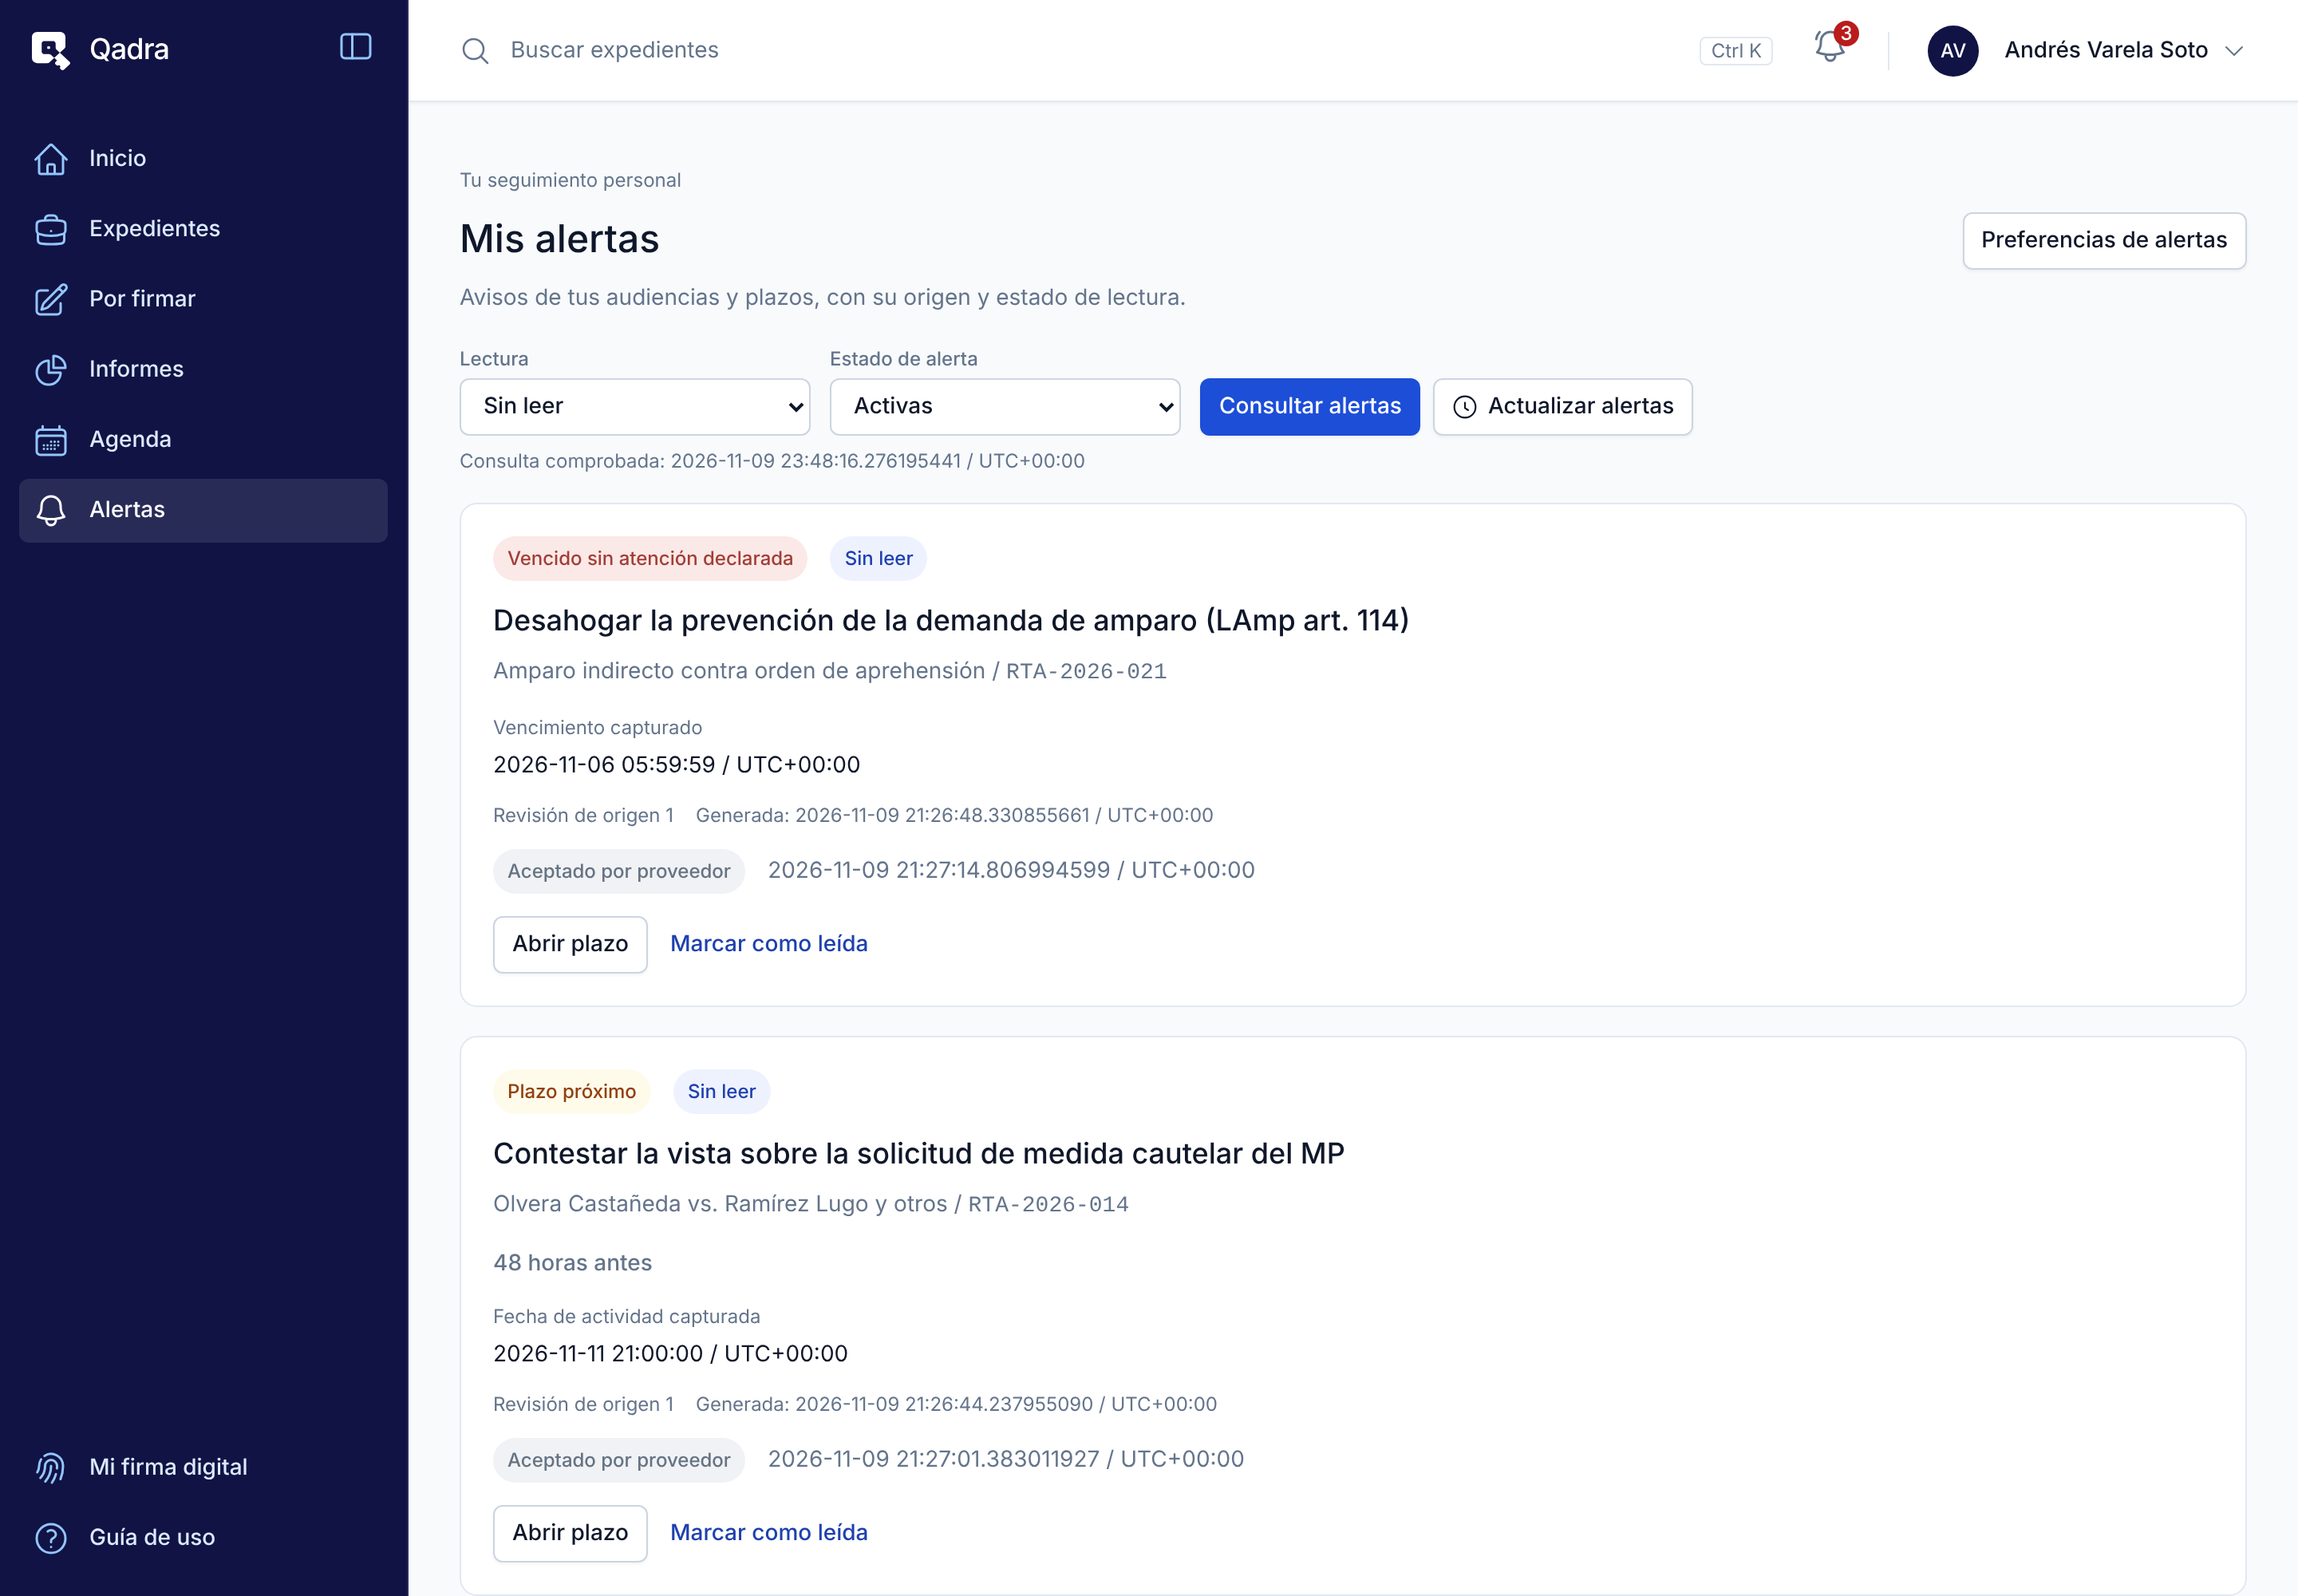
\includegraphics[width=0.9\textwidth,height=0.8\textheight,keepaspectratio]{capturas/A-35-mis-alertas.png}
  \caption{Bandeja de alertas.}
  \label{fig:manual-alertas}
\end{figure}

\resultado La alerta queda como \textbf{Leída}.

\begin{table}[H]
  \centering
  \caption{Tipos de alerta.}\label{tab:tipos-alerta}
  \begin{tabularx}{\textwidth}{L{5.2cm} Y}
    \toprule
    \textbf{Alerta} & \textbf{Cuándo aparece} \\
    \midrule
    \textbf{Audiencia próxima} (también cautelar o de recurso) & Se acerca una audiencia. \\
    \textbf{Plazo próximo}                     & Se acerca un vencimiento. \\
    \textbf{Vencido sin atención declarada}    & Venció un plazo y nadie declaró su atención. \\
    \textbf{Revisión requerida}                & Un plazo necesita que lo revise. \\
    \textbf{Fecha próxima modificada}          & Cambió la fecha de una actividad cercana. \\
    \bottomrule
  \end{tabularx}
\end{table}

\nota{Abrir una alerta no la marca como leída; use el botón
\textbf{Marcar como leída}. Leer una alerta tampoco declara la atención del
plazo.}

\subsection*{Preferencias de alertas}

\pasos
\begin{enumerate}
  \item En \textbf{Mis alertas}, vaya a \textbf{Preferencias de alertas}.
  \item Para cada grupo (\textbf{Audiencias próximas},
        \textbf{Plazos próximos}, etc.), marque si quiere avisos internos y
        por correo.
  \item En las anticipaciones, escriba con cuántas horas de anticipación
        quiere el aviso: hasta ocho valores entre 1 y 720, separados por
        comas (por ejemplo, \texttt{24, 72}).
  \item Haga clic en \textbf{Guardar preferencias}.
\end{enumerate}

\resultado Aparece \enquote{Preferencias guardadas.}

\nota{El correo solo contiene un aviso genérico y el acceso a Qadra, sin
datos del expediente. Si el servidor no tiene el correo habilitado, sus
preferencias se guardan pero no se envían correos.}

\chapter{Contratos con el Cliente}\label{cap:contratos}

Un contrato es una versión PDF que firman primero el Cliente y después una
persona del despacho, cada uno con su certificado. El recorrido completo es:

\begin{enumerate}
  \item El despacho crea el contrato y solicita las firmas
        (\cref{sec:crear-contrato}).
  \item El Cliente revisa y firma desde \textbf{Mis contratos} (\cref{sec:cliente-firmar}).
  \item El despacho comprueba la firma del Cliente y firma desde
        \textbf{Por firmar} (\cref{sec:firmar-despacho}).
\end{enumerate}

\importante{Una versión en contrato ya no admite sello ni firma personal. Si
necesita cambiar el documento, agregue una versión nueva y solicite firmas
sobre ella.}

% ---------------------------------------------------------------------
\section{Antes de solicitar firmas}\label{sec:contrato-requisitos}

Verifique que se cumplen estas condiciones; si falta alguna, Qadra
muestra la lista \textbf{Antes de solicitar las firmas} y no crea la
solicitud.

\begin{table}[H]
  \centering
  \caption{Condiciones para solicitar firmas.}\label{tab:contrato-requisitos}
  \begin{tabularx}{\textwidth}{L{3.6cm} Y}
    \toprule
    \textbf{Quién o qué} & \textbf{Condición} \\
    \midrule
    Documento & Versión actual, en PDF y sin sellar. \\
    Cliente   & Cuenta creada por invitación, activa y con su firma vinculada
                en \textbf{Mi firma digital}. \\
    Firmante del despacho & Administrador o Litigante con firma vinculada y
                vigente, y asignado al expediente. \\
    Hoja de huella & Ambas partes firmaron a mano los ejemplares de la hoja de
                huella; se necesita su folio. \\
    \bottomrule
  \end{tabularx}
\end{table}

% ---------------------------------------------------------------------
\section{Crear un contrato y solicitar firmas}\label{sec:crear-contrato}

\paraque Convierte una versión PDF en contrato y la envía a firma.

\disponible Administrador y Litigante.

\pasos
\begin{enumerate}
  \item Abra la ficha del documento PDF (\cref{sec:ficha-documental}) y
        haga clic en \textbf{Crear contrato}.
  \item Revise el \textbf{Título del contrato} y haga clic en
        \textbf{Crear contrato}. Aparece \enquote{Contrato creado en
        borrador.}
  \item En \textbf{Solicitar firmas}, escriba el
        \textbf{Correo de la cuenta del Cliente}.
  \item En \textbf{Firma por el despacho}, elija la cuenta que firmará.
  \item Indique la \textbf{Vigencia en días} (de 1 a 30) y el
        \textbf{Folio de la hoja de huella firmada}.
  \item Haga clic en \textbf{Solicitar firmas}.
\end{enumerate}

\begin{figure}[H]
  \centering
  \capturapendiente{capturas/A-36-solicitar-firmas.png}%
    {Formulario Solicitar firmas con correo del Cliente, firmante, vigencia y folio · Litigante}
  \caption{Solicitud de firmas de un contrato.}
  \label{fig:manual-solicitar-firmas}
\end{figure}

\resultado Aparece \enquote{Firmas solicitadas. Consulta su avance en
Contratos del expediente.} El Cliente ya puede firmar.

% ---------------------------------------------------------------------
\section{Seguir un contrato}\label{sec:seguir-contrato}

\paraque Muestra el estado de los contratos del expediente y permite
descargar sus paquetes.

\disponible Administrador y Litigante; el Asistente legal solo consulta.

\pasos
\begin{enumerate}
  \item En el expediente, abra la pestaña \textbf{Contratos}.
  \item Haga clic en \textbf{Abrir} junto al contrato.
  \item Revise las \textbf{Solicitudes de firma} y la
        \textbf{Línea de tiempo}.
  \item Descargue lo que necesite: \textbf{Descargar acuse parcial} (cuando
        firmó el Cliente) o \textbf{Descargar contrato firmado} (cuando
        firmaron ambos).
\end{enumerate}

\begin{figure}[H]
  \centering
  \capturapendiente{capturas/A-37-detalle-contrato.png}%
    {Detalle de un contrato con su solicitud, línea de tiempo y botones de descarga · Litigante}
  \caption{Detalle de un contrato.}
  \label{fig:manual-detalle-contrato}
\end{figure}

\begin{table}[H]
  \centering
  \caption{Estados de una solicitud de firma.}\label{tab:estados-solicitud}
  \begin{tabularx}{\textwidth}{L{5cm} Y}
    \toprule
    \textbf{Estado} & \textbf{Qué significa} \\
    \midrule
    \textbf{Espera la firma del Cliente}  & El Cliente aún no firma. \\
    \textbf{Espera la firma del despacho} & El Cliente firmó; falta el despacho. \\
    \textbf{Formalizado}                  & Firmaron ambas partes. \\
    \textbf{Rechazado por el Cliente}     & El Cliente rechazó el contrato. \\
    \textbf{Declinado por el despacho}    & El despacho no firmó; la firma del Cliente se conserva. \\
    \textbf{Cancelado} / \textbf{Vencido} & La solicitud se cerró sin formalizar. \\
    \bottomrule
  \end{tabularx}
\end{table}

\begin{itemize}
  \item Para cancelar una solicitud abierta, haga clic en
        \textbf{Cancelar solicitud}, escriba el \textbf{Motivo} y haga clic
        en \textbf{Confirmar cancelación}.
  \item Un contrato en \textbf{Borrador} sin solicitud puede abandonarse con
        \textbf{Abandonar contrato}.
  \item Solo puede haber una solicitud abierta por contrato.
\end{itemize}

% ---------------------------------------------------------------------
\section{Firmar por el despacho}\label{sec:firmar-despacho}

\paraque Contrafirma el contrato después del Cliente y lo formaliza.

\disponible La cuenta elegida en \textbf{Firma por el despacho}
(Administrador o Litigante).

Tenga a la mano su clave privada cifrada (archivo \texttt{.pem}) y su
contraseña.

\pasos
\begin{enumerate}
  \item En el menú, haga clic en \textbf{Por firmar} y elija la solicitud.
  \item En \textbf{1. Revisa}, haga clic en
        \textbf{Cargar y comprobar el PDF} y lea el contrato.
  \item En \textbf{Comprueba la firma del Cliente}, haga clic en
        \textbf{Descargar acuse parcial}. Seleccione ese archivo en el
        validador y haga clic en \textbf{Validar paquete}.
  \item En \textbf{2. Confirma}, marque \textbf{Confirmo firmar por el
        despacho esta versión exacta, después de revisar la firma del
        Cliente.}
  \item En \textbf{3. Firma}, haga clic en \textbf{Preparar la firma}.
        Seleccione su \textbf{Clave privada cifrada}, escriba la
        \textbf{Contraseña de la clave} y haga clic en
        \textbf{Firmar localmente}.
  \item Haga clic en \textbf{Enviar firma}.
\end{enumerate}

\begin{figure}[H]
  \centering
  \capturapendiente{capturas/A-38-por-firmar.png}%
    {Por firmar con los pasos 1. Revisa, 2. Confirma y 3. Firma y el acuse parcial validado · Litigante}
  \caption{Firma del contrato por el despacho.}
  \label{fig:manual-por-firmar}
\end{figure}

\resultado Aparece \enquote{Firma del despacho registrada; el contrato quedó
formalizado.} Descargue el paquete con \textbf{Descargar contrato firmado}.

\begin{itemize}
  \item El botón de firma se habilita solo cuando el acuse parcial se valida
        sin fallas.
  \item Si intenta firmar antes que el Cliente, aparece \enquote{No es tu
        turno de firmar. Primero firma el Cliente y después el despacho.}
  \item Si no desea firmar, haga clic en \textbf{Declinar firma}.
  \item Si se pierde la respuesta, haga clic en
        \textbf{Consultar recibo de firma}; consultar no vuelve a enviar la
        firma.
\end{itemize}

\chapter{Informes}\label{cap:informes}

\paraque Genera un informe en PDF y CSV sobre el estado de los expedientes o
la actividad de cada litigante en un periodo.

\disponible Administrador (todo el despacho) y Litigante (sus expedientes
asignados).

\begin{table}[H]
  \centering
  \caption{Tipos de informe.}\label{tab:tipos-informe}
  \begin{tabularx}{\textwidth}{L{4.8cm} Y}
    \toprule
    \textbf{Informe} & \textbf{Qué incluye} \\
    \midrule
    \textbf{Estado y carga de expedientes}
      & Expedientes creados en el periodo, su estado y el litigante
        asignado. \\
    \textbf{Actividad por litigante}
      & Documentos cargados, actuaciones registradas y plazos atendidos por
        cada litigante en el periodo. \\
    \bottomrule
  \end{tabularx}
\end{table}

\pasos
\begin{enumerate}
  \item En el menú, haga clic en \textbf{Informes}.
  \item En \textbf{Solicitar informe}, elija el tipo de informe.
  \item Indique el periodo: \textbf{Creación desde (UTC)} y
        \textbf{Creación hasta (excluida, UTC)}, o bien
        \textbf{Actividad desde (UTC)} y
        \textbf{Actividad hasta (excluida, UTC)}, según el tipo. El primer
        día se incluye y el último no; el periodo máximo es de 366 días.
  \item Si lo desea, filtre por \textbf{Estado administrativo} y por
        litigante.
  \item Haga clic en \textbf{Generar informe}.
  \item En \textbf{Solicitudes y avisos}, espere a que el estado cambie a
        \textbf{Disponible} y haga clic en \textbf{Consultar informe}.
  \item Haga clic en \textbf{Descargar PDF} o \textbf{Descargar CSV}.
\end{enumerate}

\begin{figure}[H]
  \centering
  \capturapendiente{capturas/A-39-informes.png}%
    {Informes de expedientes con la solicitud y un informe Disponible con Descargar PDF y CSV · Litigante}
  \caption{Solicitud y descarga de un informe.}
  \label{fig:manual-informes}
\end{figure}

\resultado Descarga el informe en el formato elegido. El PDF y el CSV
provienen de la misma captura de datos.

\begin{itemize}
  \item El informe se genera en el servidor; no necesita mantener la
        pantalla abierta.
  \item Las fechas del periodo se interpretan en UTC.
  \item Si el informe es demasiado grande, aparece \enquote{El informe supera
        el límite permitido. Solicita otro con un periodo o filtro más
        reducido.}
\end{itemize}

\nota{El informe muestra el estado al momento de generarlo; no reconstruye
el estado pasado del expediente ni califica resultados jurídicos.}

\chapter{Mi firma digital}\label{cap:mi-firma-digital}

En \textbf{Mi firma digital} usted prepara la clave y el certificado con los
que firma documentos y contratos. El recorrido completo es:

\begin{enumerate}
  \item Generar su clave y su solicitud de certificado (CSR) en el navegador.
  \item Guardar la clave cifrada y comprobar la copia.
  \item Imprimir la hoja de huella y entregar la solicitud al responsable de
        la autoridad certificadora (CA) del despacho.
  \item Recibir su certificado y vincularlo a su cuenta.
\end{enumerate}

\disponible Administrador, Litigante y Cliente.

\importante{Su clave privada y su contraseña nunca salen de su equipo. Qadra
no puede recuperarlas: si las pierde, deberá generar una clave nueva. Los
certificados son de la CA interna del despacho y no sustituyen a la e.firma
del SAT.}

% ---------------------------------------------------------------------
\section{Generar la clave y la solicitud}\label{sec:generar-clave}

\paraque Crea su clave privada protegida con contraseña y la solicitud
pública (CSR) que necesita la CA para emitir su certificado.

\pasos
\begin{enumerate}
  \item En el menú, haga clic en \textbf{Mi firma digital}. Si es
        Administrador, quédese en la pestaña \textbf{Firma de documentos}.
  \item En \textbf{Generar clave y solicitud}, llene
        \textbf{Datos de la solicitud}: \textbf{Nombre común (CN)},
        \textbf{Organización (O)} y \textbf{País (C)} (por ejemplo,
        \texttt{MX}).
  \item Escriba la \textbf{Contraseña de la nueva clave} (al menos 12
        caracteres) y repítala en \textbf{Confirmar contraseña}.
  \item Haga clic en \textbf{Generar clave y solicitud}.
  \item Haga clic en \textbf{Descargar clave cifrada} y guarde el archivo
        \archivo{qadra-document-signing-key.encrypted.pem} en un lugar seguro.
  \item Para comprobar la copia, selecciónela en
        \textbf{Archivo de clave cifrada guardado}, escriba su contraseña en
        \textbf{Contraseña de la clave guardada} y haga clic en
        \textbf{Comprobar copia guardada}.
  \item Haga clic en \textbf{Descargar solicitud CSR}. Se descarga
        \archivo{qadra-document-signing-request.csr.pem}.
\end{enumerate}

\begin{figure}[H]
  \centering
  \capturapendiente{capturas/A-40-generar-clave.png}%
    {Sección Generar clave y solicitud con Datos de la solicitud y contraseña · Litigante}
  \caption{Generación de la clave y la solicitud.}
  \label{fig:manual-generar-clave}
\end{figure}

\resultado Aparece \enquote{La copia cifrada se puede abrir y corresponde a
esta solicitud.} y queda descargada su solicitud CSR.

\nota{El nombre que escribe es declarado: no acredita su identidad. Para el
Cliente, la organización es fija y corresponde a la CA emisora.}

% ---------------------------------------------------------------------
\section{Hoja de huella y entrega de la solicitud}\label{sec:hoja-huella}

\paraque Asegura que el certificado que emitirá la CA corresponde a la clave
que usted generó.

\pasos
\begin{enumerate}
  \item En \textbf{Huella de tu clave pública}, haga clic en
        \textbf{Imprimir hoja de huella}.
  \item Imprima la \textbf{Hoja de huella de firma documental}. Tiene dos
        ejemplares: \textbf{Ejemplar del Cliente} y
        \textbf{Ejemplar del despacho}.
  \item Firmen a mano ambos ejemplares (usted y el despacho). Anote el
        \textbf{Folio}; se pide al solicitar las firmas de un contrato.
  \item Entregue solo el archivo CSR al responsable de la CA.
  \item Lea la huella al responsable de la CA, en persona o por teléfono.
        Debe coincidir con la que él ve antes de emitir el certificado.
\end{enumerate}

\begin{figure}[H]
  \centering
  \capturapendiente{capturas/A-41-hoja-huella.png}%
    {Vista de impresión de la Hoja de huella de firma documental con ambos ejemplares (datos de prueba) · Litigante}
  \caption{Hoja de huella de firma documental.}
  \label{fig:manual-hoja-huella}
\end{figure}

\resultado La CA le entrega su certificado público (archivo \texttt{.pem}).

\importante{Comparta solo el CSR. Nunca entregue su clave privada ni su
contraseña, ni siquiera al responsable de la CA.}

% ---------------------------------------------------------------------
\section{Registrar el certificado y el vínculo}\label{sec:registrar-vinculo}

\paraque Vincula su certificado a su cuenta de Qadra. Sin vínculo no puede
firmar documentos ni contratos.

\pasos
\begin{enumerate}
  \item En \textbf{Mi firma digital}, vaya a
        \textbf{Registrar certificado documental}.
  \item Seleccione su certificado en \textbf{Certificado público PEM} y haga
        clic en \textbf{Preparar vínculo}.
  \item Revise los datos del certificado.
  \item En \textbf{Firmar en este dispositivo}, seleccione su
        \textbf{Clave privada cifrada}, escriba la
        \textbf{Contraseña de la clave} y haga clic en
        \textbf{Firmar localmente}.
  \item Marque \textbf{Confirmo vincular este certificado a mi cuenta}.
  \item Haga clic en \textbf{Registrar vínculo}.
\end{enumerate}

\begin{figure}[H]
  \centering
  \capturapendiente{capturas/A-42-registrar-vinculo.png}%
    {Registrar certificado documental con certificado cargado y Firmar en este dispositivo · Litigante}
  \caption{Registro del vínculo del certificado.}
  \label{fig:manual-registrar-vinculo}
\end{figure}

\resultado Aparece \textbf{Vínculo registrado}. Haga clic en
\textbf{Descargar recibo del vínculo} para conservar el recibo
(\archivo{certificate-binding-receipt.json}).

\nota{Si prefiere firmar con su propia herramienta, abra
\textbf{Usar una firma externa}, descargue la declaración con
\textbf{Descargar declaración del vínculo}, fírmela y cargue el resultado en
\textbf{Firma externa del vínculo}.}

% ---------------------------------------------------------------------
\section{Retirar el vínculo}\label{sec:retirar-vinculo}

\paraque Deja de usar un certificado, por ejemplo si perdió su clave o va a
renovarlo.

\importante{Retirar el vínculo impide firmar con ese certificado en adelante.
Las firmas anteriores conservan su evidencia.}

\pasos
\begin{enumerate}
  \item En \textbf{Vínculo registrado}, haga clic en \textbf{Retirar vínculo}.
  \item Marque \textbf{Confirmo retirar el vínculo para futuras firmas}.
  \item Haga clic en \textbf{Confirmar retiro}.
\end{enumerate}

\resultado Aparece \textbf{Vínculo retirado}. Para volver a firmar, genere
una clave nueva o registre un certificado renovado.

% ---------------------------------------------------------------------
\section{Certificado vencido o por vencer}\label{sec:certificado-vence}

Qadra le avisa en \textbf{Mi firma digital}:

\begin{itemize}
  \item \textbf{Por vencer:} \enquote{Tu certificado vence en menos de 30
        días. Renuévalo y vuelve a vincularlo; una solicitud abierta con el
        certificado anterior debe rehacerse.}
  \item \textbf{Vencido:} \enquote{Tu certificado venció. Genera una clave
        nueva o renueva el certificado y vuelve a vincularlo.}
\end{itemize}

En ambos casos, repita las \cref{sec:generar-clave,sec:hoja-huella,sec:registrar-vinculo}.

% ---------------------------------------------------------------------
\section{Certificado para ingresar (Administrador)}\label{sec:acceso-certificado}

\paraque Registra el certificado con el que el Administrador puede entrar a
Qadra (\cref{sec:ingresar-certificado}). Este certificado no firma
documentos.

\disponible Administrador.

\pasos
\begin{enumerate}
  \item En \textbf{Mi firma digital}, abra la pestaña
        \textbf{Acceso con certificado}.
  \item Genere su clave y su solicitud igual que en la
        \cref{sec:generar-clave}, y obtenga su certificado de la CA.
  \item Haga clic en \textbf{Registrar certificado}.
  \item Seleccione su \textbf{Certificado público PEM} y haga clic en
        \textbf{Preparar vínculo}.
  \item Firme en \textbf{Firmar en este dispositivo} con su clave y su
        contraseña, y haga clic en \textbf{Registrar vínculo}.
  \item En \textbf{Vínculo de mi cuenta}, haga clic en
        \textbf{Descargar recibo}. Ese archivo \texttt{.json} es el que
        seleccionará al ingresar con certificado.
\end{enumerate}

\begin{figure}[H]
  \centering
  \capturapendiente{capturas/A-43-acceso-certificado.png}%
    {Pestaña Acceso con certificado con Vínculo de mi cuenta y Descargar recibo · Administrador}
  \caption{Certificado para ingresar a Qadra.}
  \label{fig:manual-acceso-certificado}
\end{figure}

\resultado El vínculo aparece como \textbf{Sin retirar} y ya puede usar
\textbf{Ingresar con certificado}.

\nota{Para dejar de usarlo, haga clic en \textbf{Retirar vínculo} y luego en
\textbf{Confirmar retiro}. El retiro es definitivo para ese vínculo y cierra
las sesiones abiertas con él; su acceso con contraseña y segundo factor no
cambia.}

\chapter{Funciones del Administrador}\label{cap:administracion}

\disponible Solo Administrador. Estas opciones aparecen en el menú bajo
\textbf{Administración}, y la pestaña \textbf{Asignaciones} dentro de cada
expediente.

% ---------------------------------------------------------------------
\section{Invitar a un integrante}\label{sec:invitar}

\paraque Envía un enlace privado por correo para que la persona cree su
propia cuenta (\cref{sec:aceptar-invitacion}).

\pasos
\begin{enumerate}
  \item En el menú, haga clic en \textbf{Equipo}.
  \item En \textbf{Invitaciones al despacho}, escriba el
        \textbf{Nombre de la persona invitada} y el
        \textbf{Correo de la invitación}.
  \item Elija el \textbf{Rol de la invitación}: \textbf{Asistente legal},
        \textbf{Litigante} o \textbf{Cliente}.
  \item Haga clic en \textbf{Enviar invitación}.
\end{enumerate}

\begin{figure}[H]
  \centering
  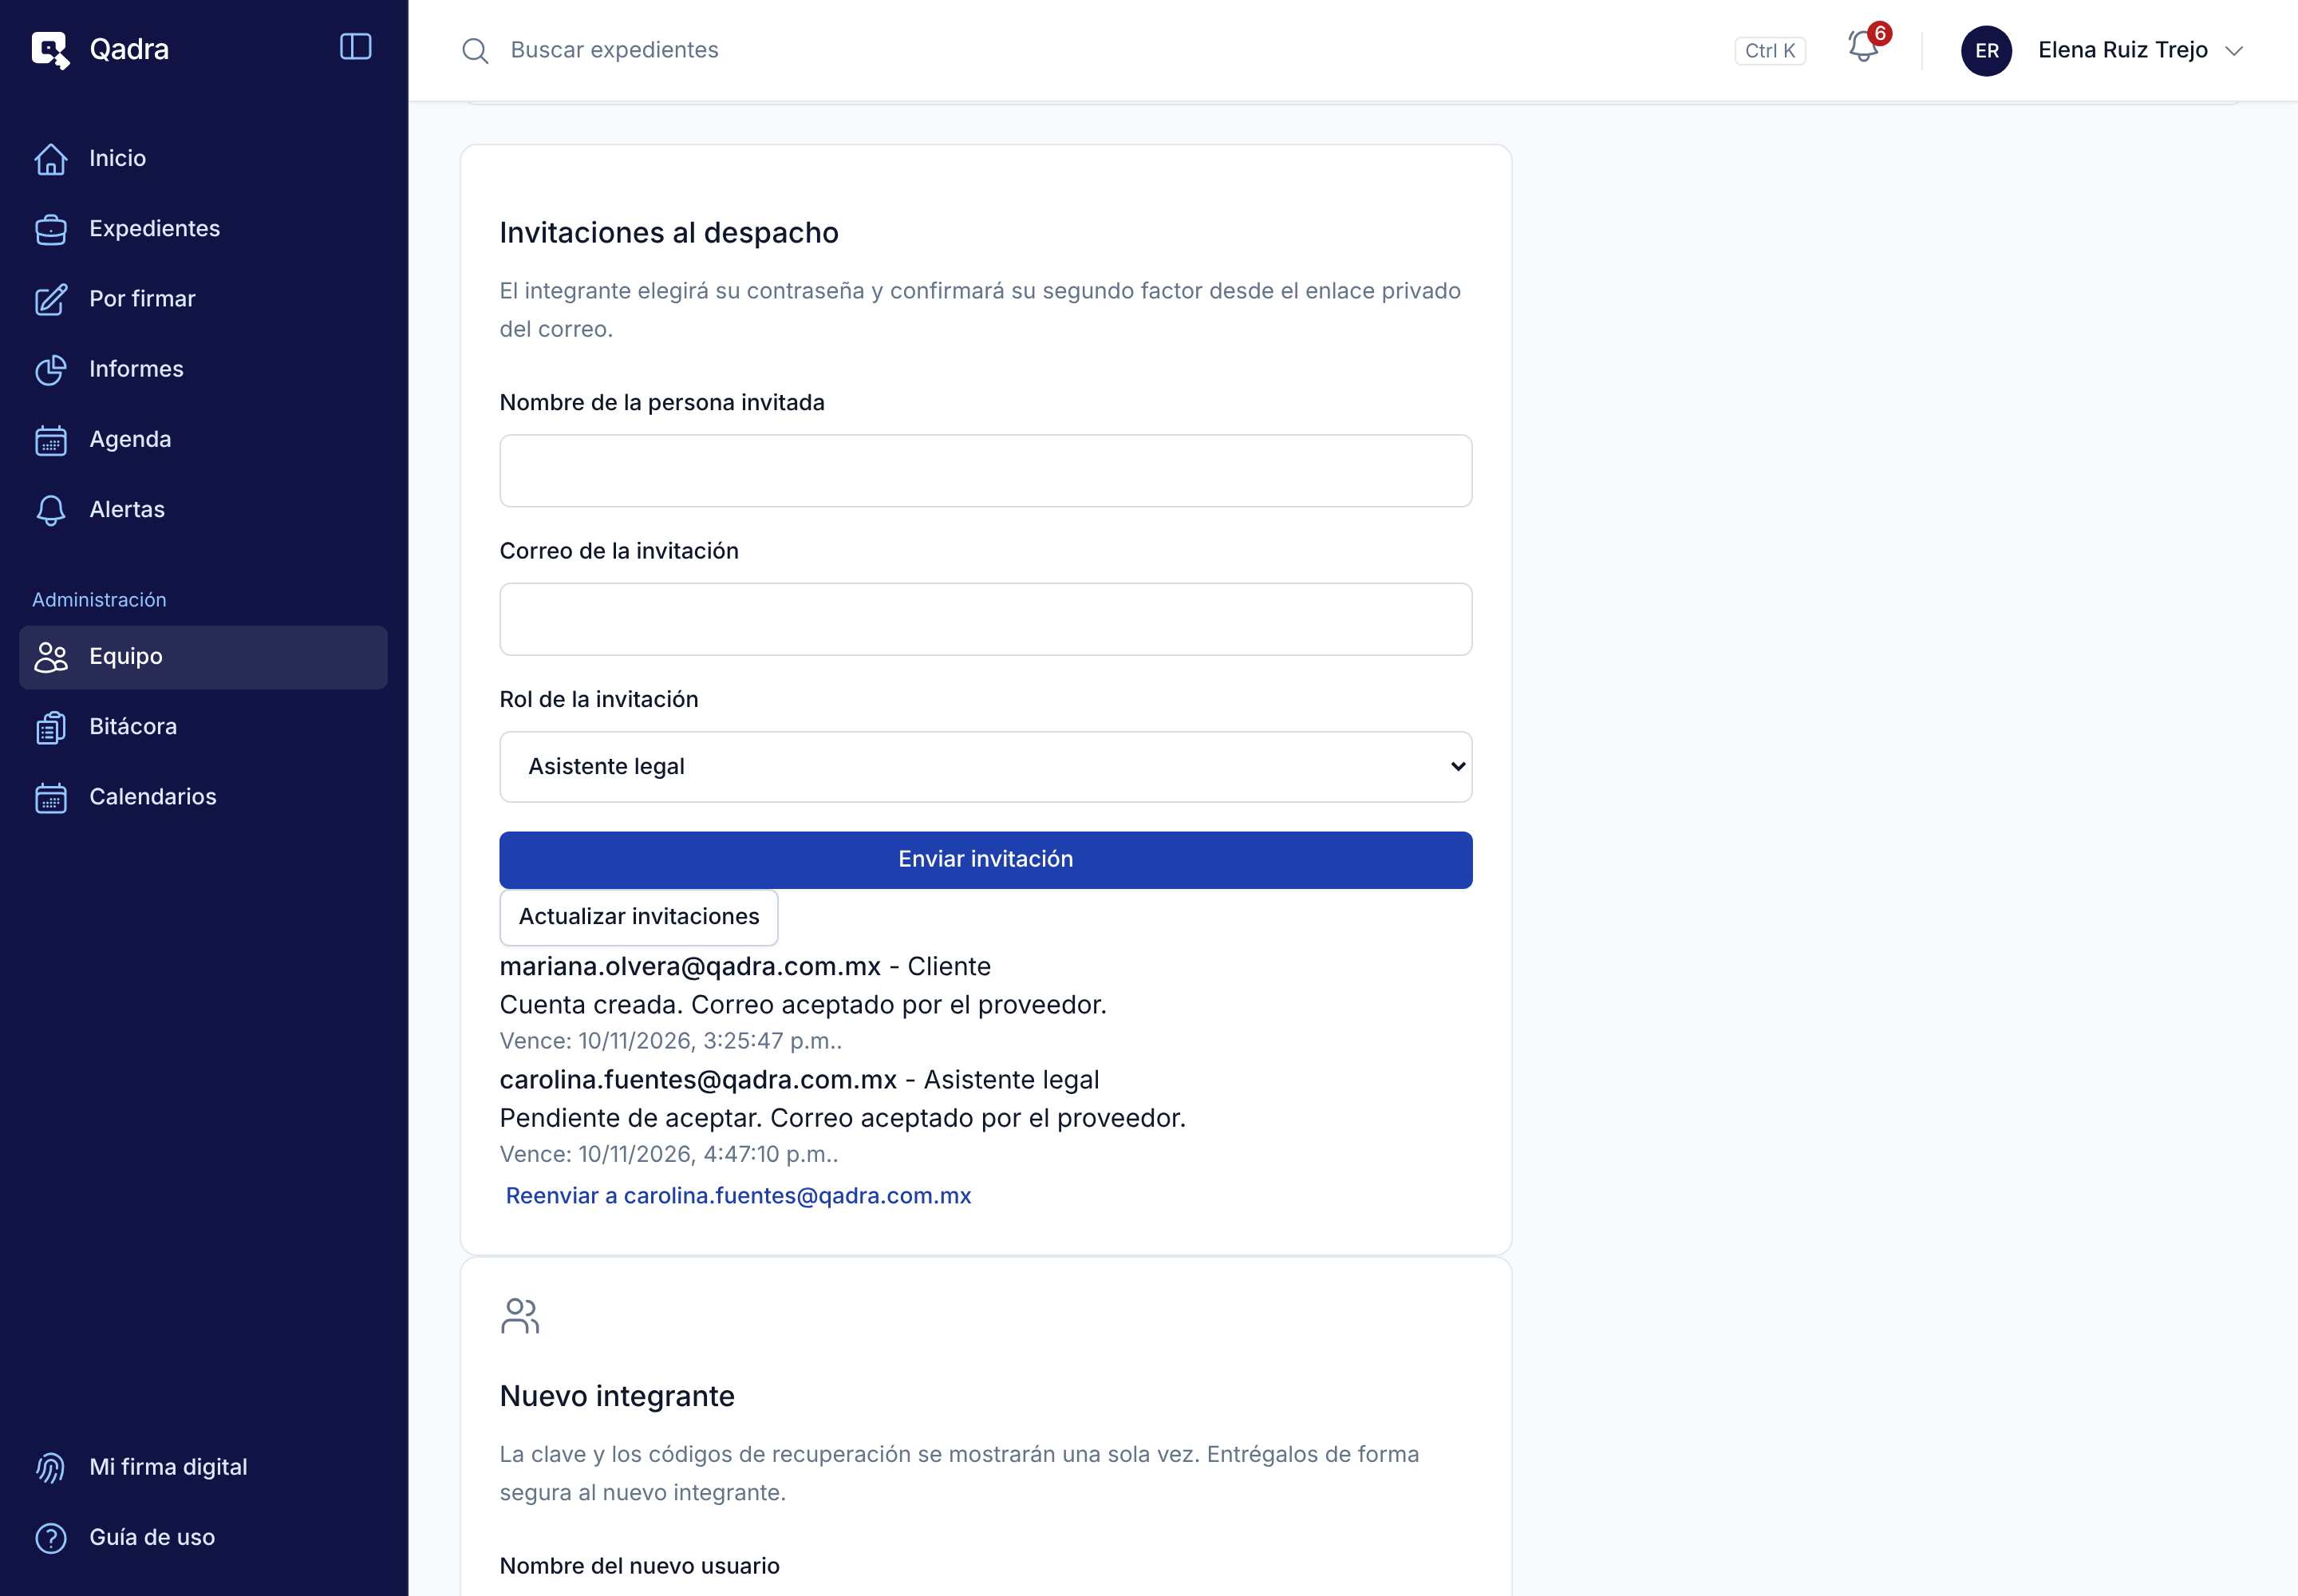
\includegraphics[width=0.9\textwidth]{capturas/A-44-invitaciones.png}
  \caption{Invitaciones al despacho.}
  \label{fig:manual-invitaciones}
\end{figure}

\resultado Aparece \enquote{Invitación registrada para [correo].} y la
invitación se agrega a la lista con su estado y fecha de vencimiento.

\begin{table}[H]
  \centering
  \caption{Estados de una invitación.}\label{tab:estados-invitacion}
  \begin{tabularx}{\textwidth}{L{5.2cm} Y}
    \toprule
    \textbf{Estado} & \textbf{Qué significa} \\
    \midrule
    \textbf{Pendiente de aceptar}        & La persona aún no abre el enlace. \\
    \textbf{Pendiente de confirmar MFA}  & Eligió su contraseña, pero no ha confirmado su segundo factor. \\
    \textbf{Cuenta creada}               & La cuenta ya existe. \\
    \textbf{Enlace vencido o retirado}   & El enlace ya no funciona; reenvíe la invitación. \\
    \bottomrule
  \end{tabularx}
\end{table}

\begin{itemize}
  \item Para enviar un enlace nuevo, haga clic en
        \textbf{Reenviar a [correo]} y luego en \textbf{Confirmar reenvío}.
        El enlace anterior deja de funcionar.
  \item La lista también indica la entrega del correo, por ejemplo
        \textbf{Correo aceptado por el proveedor} o
        \textbf{Correo rechazado}.
\end{itemize}

% ---------------------------------------------------------------------
\section{Dar de alta a un integrante directamente}\label{sec:alta-directa}

\paraque Crea una cuenta sin correo de invitación. También permite crear otro
Administrador.

\pasos
\begin{enumerate}
  \item En \textbf{Equipo}, vaya a \textbf{Nuevo integrante}.
  \item Escriba el \textbf{Nombre del nuevo usuario}, el
        \textbf{Correo del nuevo usuario} y una \textbf{Contraseña inicial}
        de al menos 12 caracteres.
  \item Elija el \textbf{Rol}: \textbf{Asistente legal},
        \textbf{Litigante}, \textbf{Administrador} o \textbf{Cliente}.
  \item Haga clic en \textbf{Crear usuario}. Para abandonar el alta, use
        \textbf{Descartar alta y volver al directorio}.
  \item En \textbf{Configura el segundo factor}, copie la
        \textbf{Clave de configuración} y los
        \textbf{Códigos de recuperación}.
  \item Marque \textbf{Ya guardé la clave y los códigos} y haga clic en
        \textbf{Finalizar}.
\end{enumerate}

\begin{figure}[H]
  \centering
  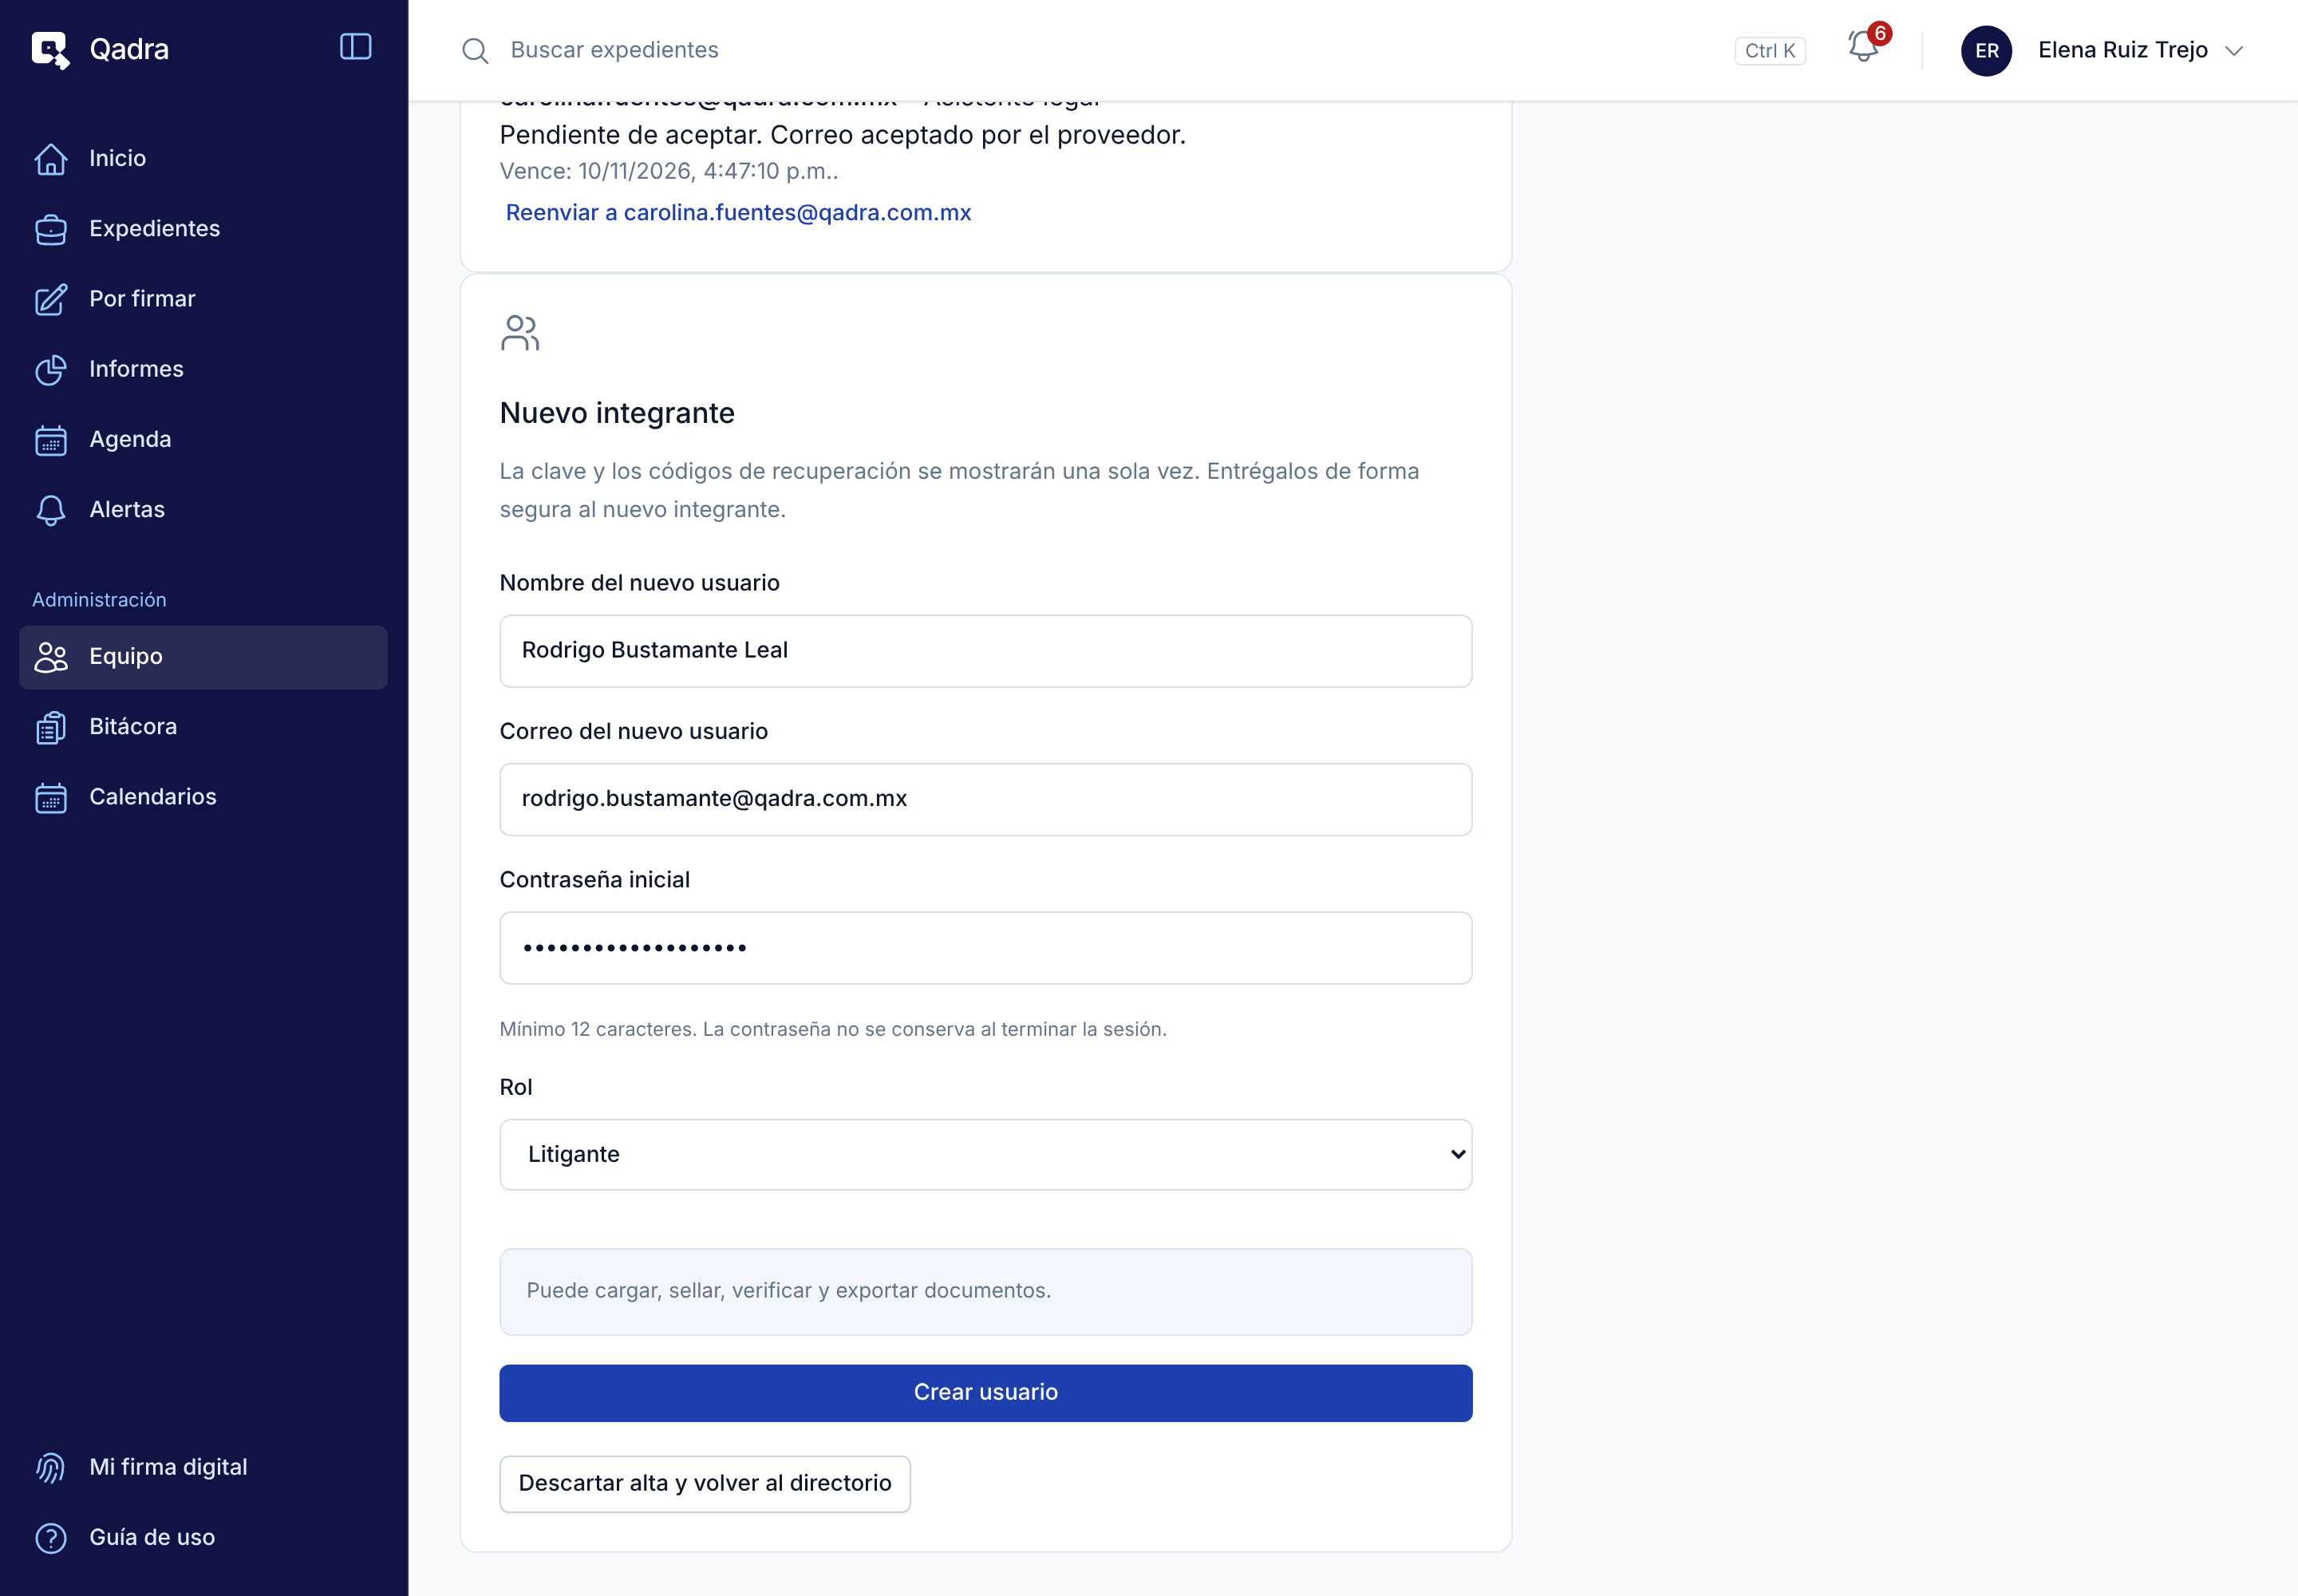
\includegraphics[width=0.9\textwidth]{capturas/A-45-nuevo-integrante.png}
  \caption{Alta directa de un integrante.}
  \label{fig:manual-nuevo-integrante}
\end{figure}

\resultado La cuenta aparece en el \textbf{Directorio de cuentas}.

\importante{La clave y los códigos se muestran una sola vez. Entréguelos al
nuevo integrante por un medio seguro, junto con su contraseña inicial.}

% ---------------------------------------------------------------------
\section{Cambiar el rol o desactivar una cuenta}\label{sec:administrar-acceso}

\paraque Cambia el rol de una cuenta o la desactiva para bloquear su acceso.

\pasos
\begin{enumerate}
  \item En \textbf{Equipo}, vaya a \textbf{Directorio de cuentas}. Si es
        necesario, use \textbf{Buscar por correo}, \textbf{Rol de la cuenta}
        o \textbf{Estado de la cuenta} y haga clic en
        \textbf{Buscar cuentas}.
  \item Haga clic en \textbf{Administrar acceso de [correo]}.
  \item Elija el nuevo \textbf{Rol de la cuenta} o el
        \textbf{Estado de la cuenta} (\textbf{Activa} o \textbf{Inactiva}).
  \item Haga clic en \textbf{Revisar acceso}. En
        \textbf{Confirmar los permisos seleccionados} revise el cambio
        (por ejemplo, \enquote{Asistente legal / Activa a Litigante / Activa.})
        y haga clic en \textbf{Confirmar cambio de acceso}; para corregirlo,
        use \textbf{Editar selección}.
\end{enumerate}

\begin{figure}[H]
  \centering
  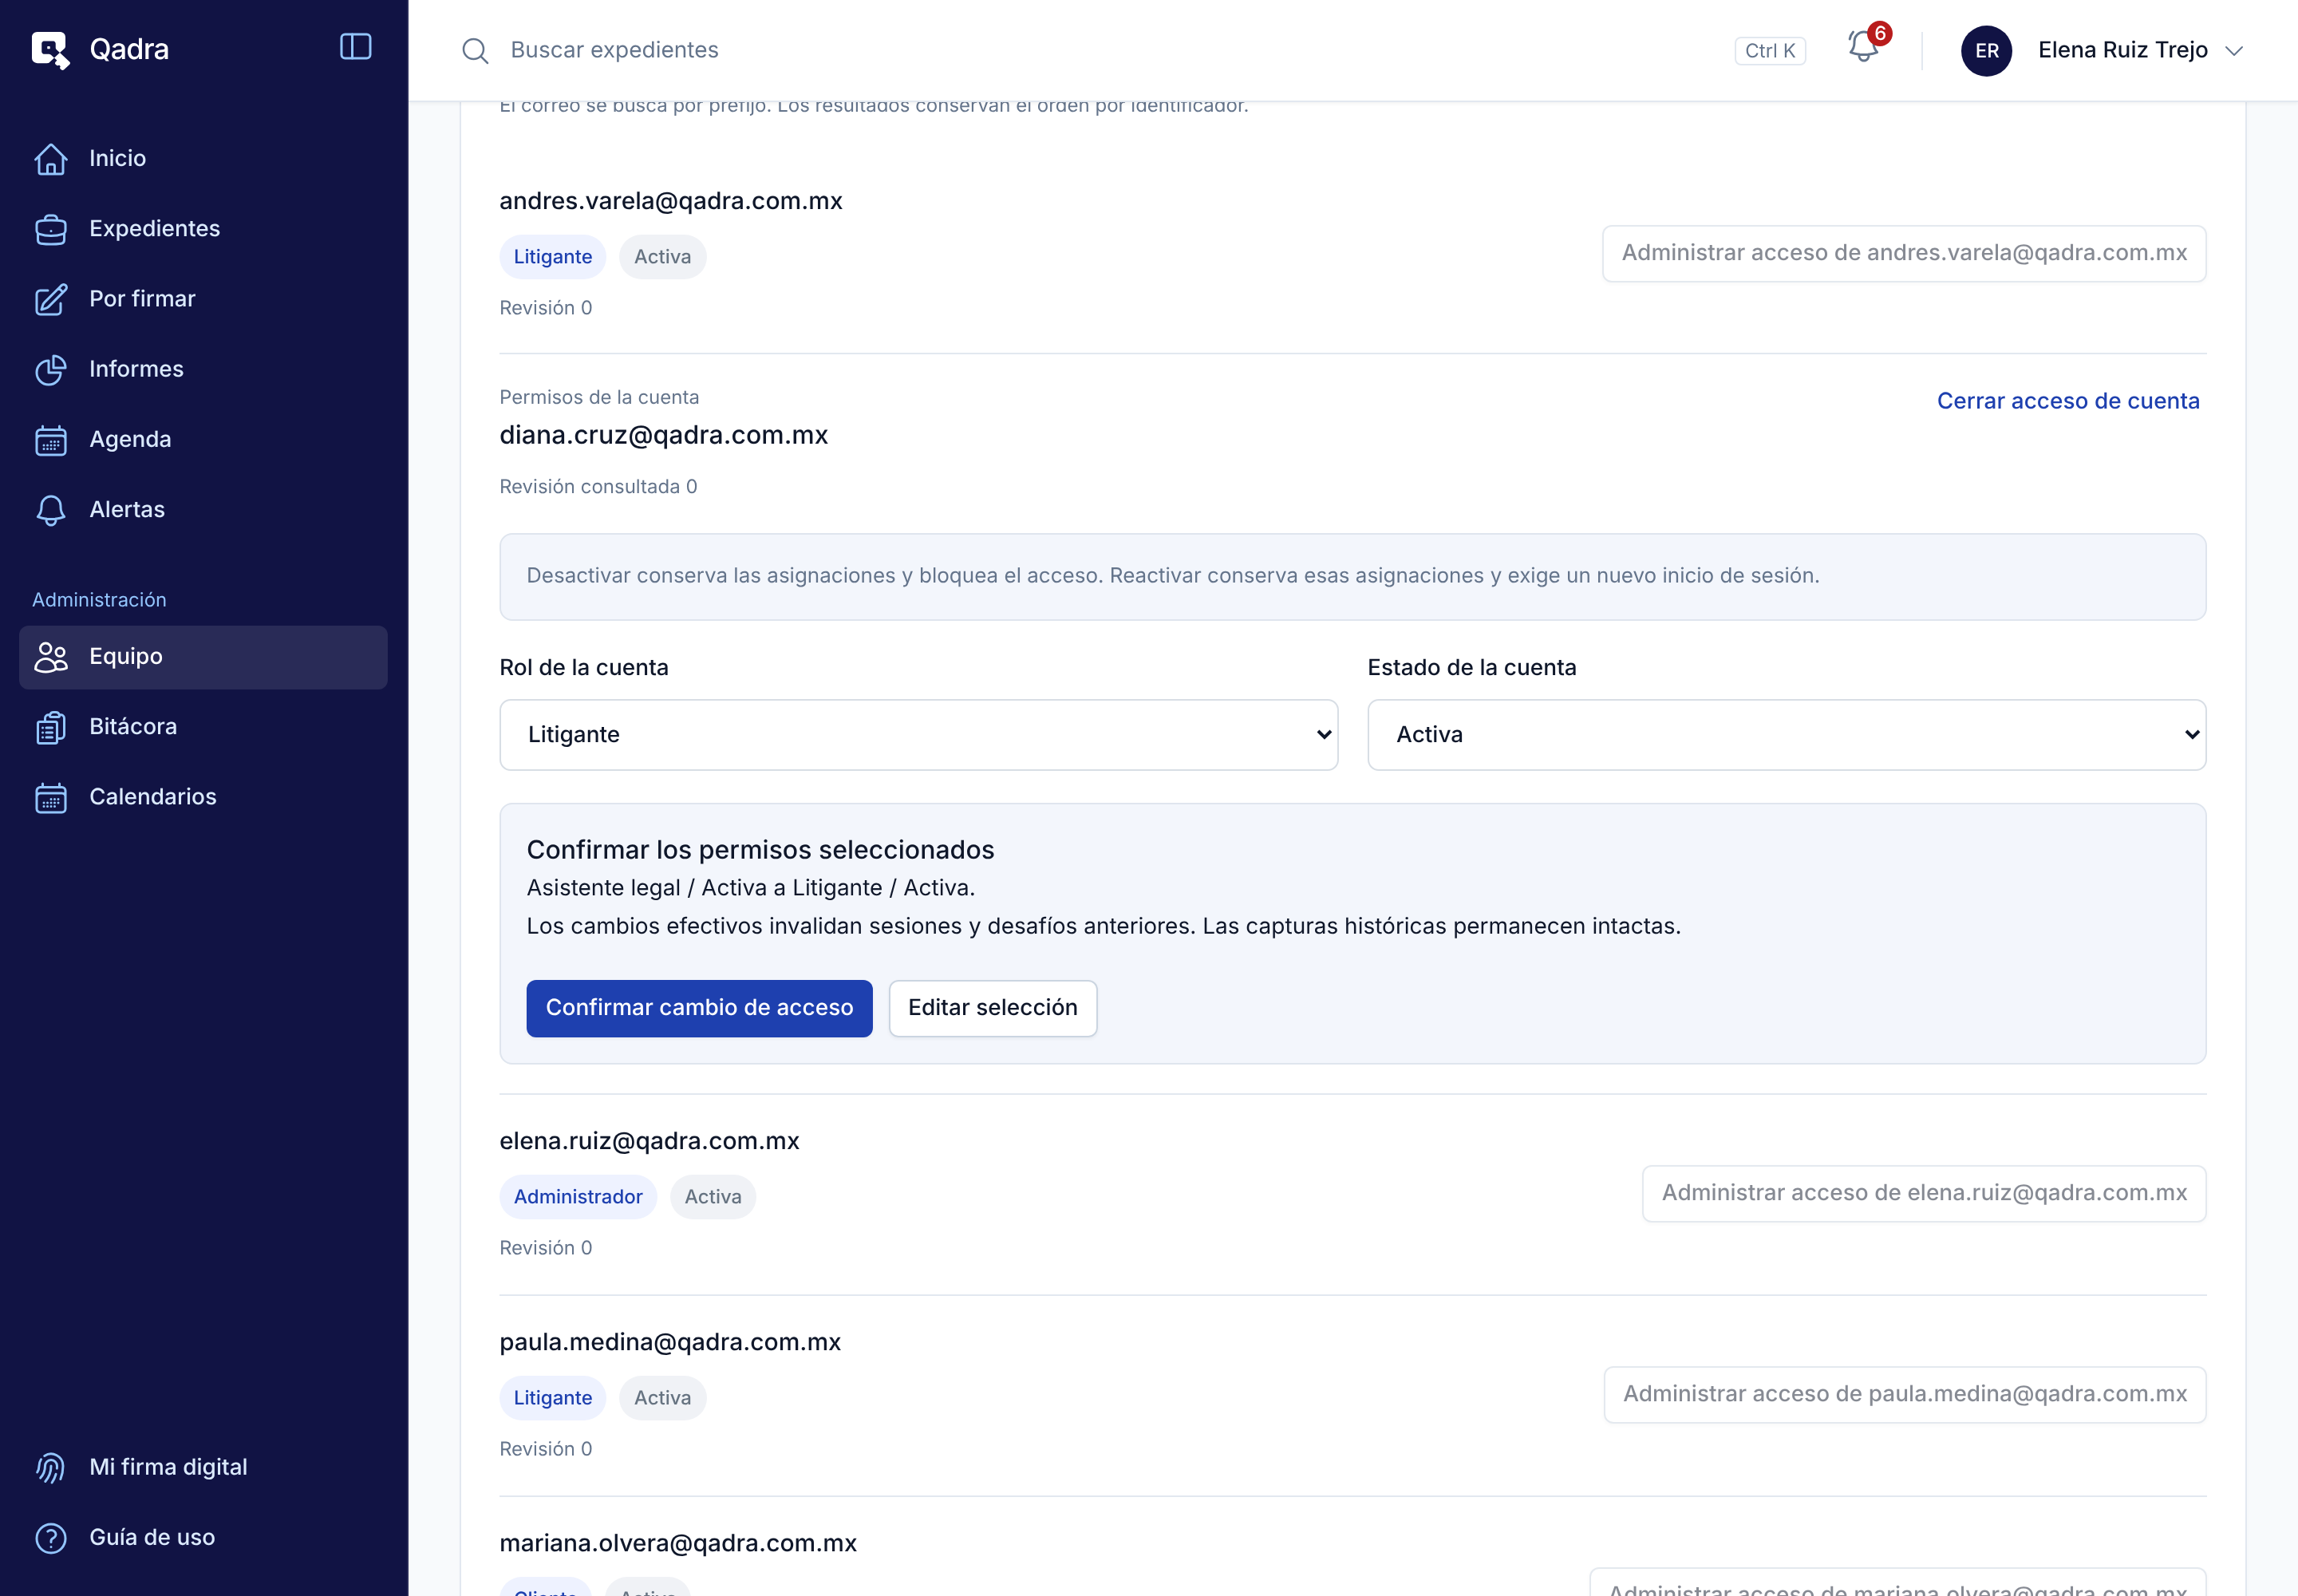
\includegraphics[width=0.9\textwidth]{capturas/A-46-administrar-acceso.png}
  \caption{Cambio de acceso de una cuenta.}
  \label{fig:manual-administrar-acceso}
\end{figure}

\resultado Aparece \enquote{Los permisos de la cuenta se confirmaron.} Las
sesiones anteriores de esa cuenta se cierran.

\begin{itemize}
  \item Desactivar conserva las asignaciones de la cuenta, pero bloquea su
        acceso. Al reactivarla, la persona debe iniciar sesión de nuevo.
  \item \textbf{Cerrar acceso de cuenta} cierra el editor sin cambios.
  \item Siempre debe quedar al menos un Administrador activo; Qadra no
        permite retirar al último.
  \item Si cambia su propio rol o estado, su sesión se cerrará.
\end{itemize}

% ---------------------------------------------------------------------
\section{Asignar cuentas a un expediente}\label{sec:asignaciones}

\paraque Da o retira a un Litigante, Asistente legal o Cliente el acceso a un
expediente.

\pasos
\begin{enumerate}
  \item Abra el expediente y haga clic en la pestaña \textbf{Asignaciones}.
  \item En \textbf{Selección de cuentas}, elija \textbf{Cuentas disponibles}
        (para asignar) o \textbf{Cuentas asignadas} (para retirar). Haga clic
        en \textbf{Buscar asignaciones}.
  \item Haga clic en \textbf{Asignar} o \textbf{Retirar} en la tarjeta de la
        cuenta.
  \item Haga clic en \textbf{Confirmar asignación} o
        \textbf{Confirmar retiro}.
\end{enumerate}

\begin{figure}[H]
  \centering
  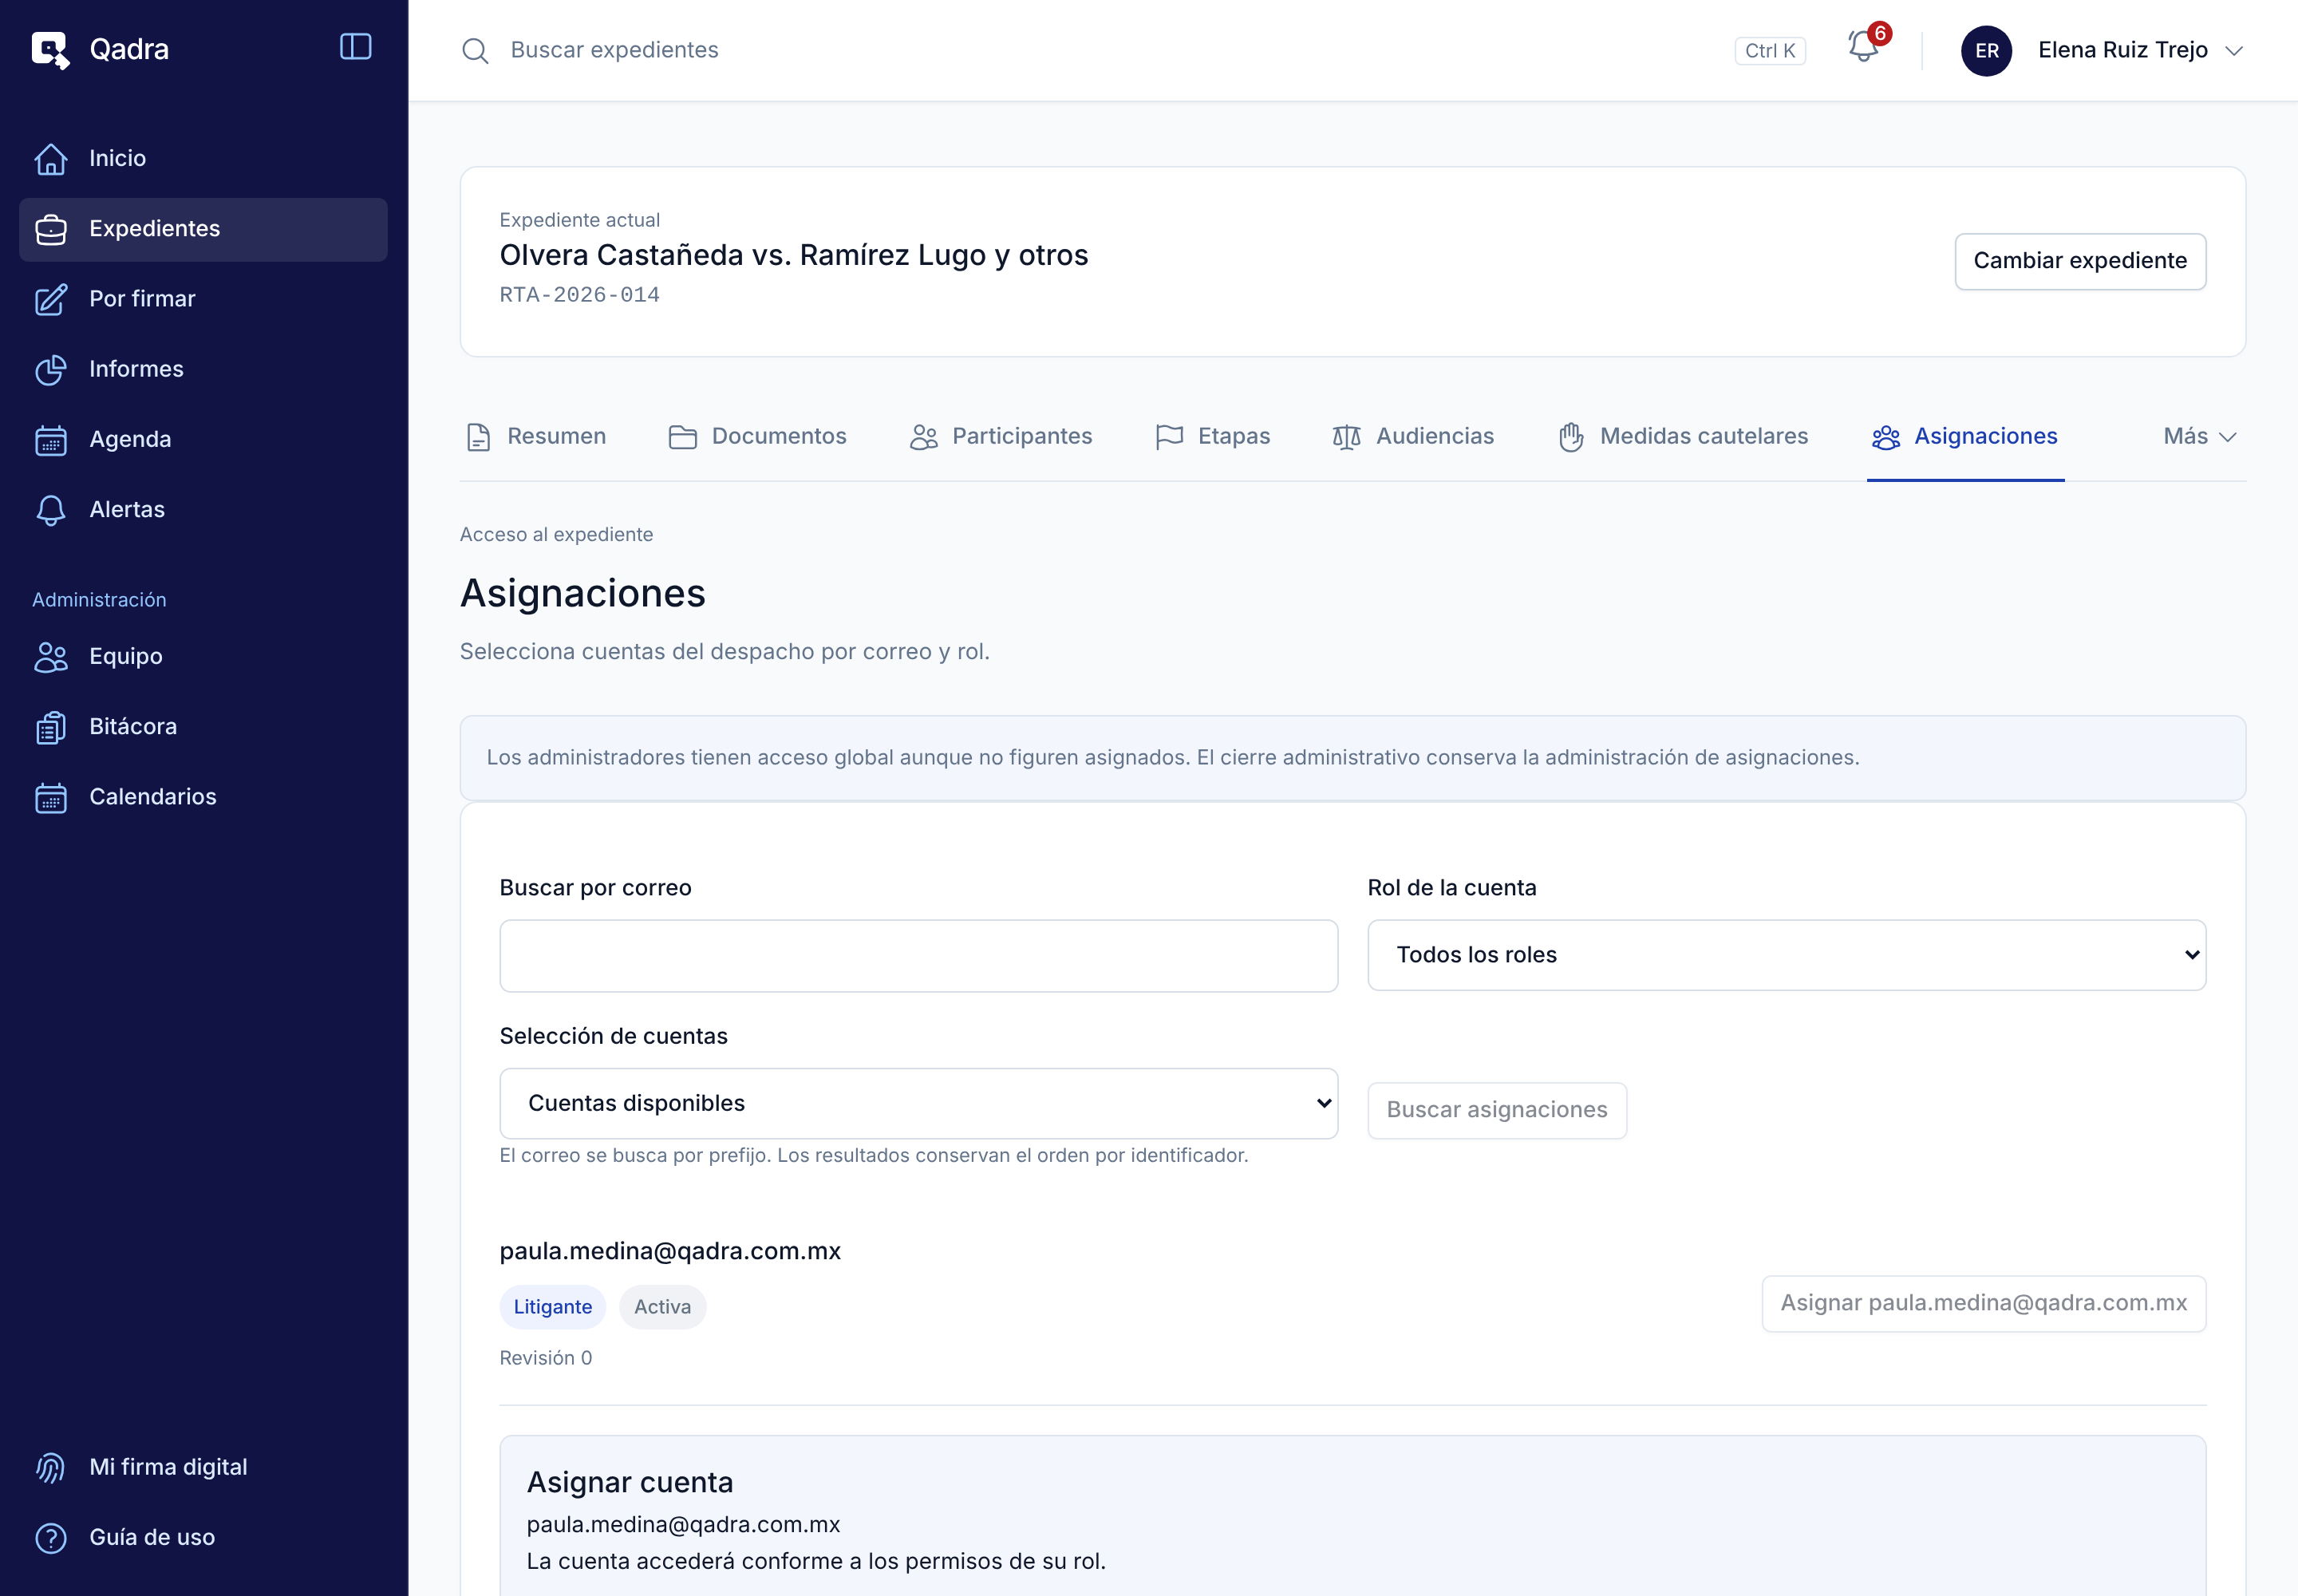
\includegraphics[width=0.9\textwidth]{capturas/A-47-asignaciones.png}
  \caption{Asignación de una cuenta a un expediente.}
  \label{fig:manual-asignaciones}
\end{figure}

\resultado Aparece \enquote{Asignación confirmada.} o \enquote{Retiro de
asignación confirmado.}

\nota{Los Administradores tienen acceso a todos los expedientes aunque no
estén asignados. Retirar una asignación conserva la cuenta y su historial.}

% ---------------------------------------------------------------------
\section{Bitácora e incidentes de integridad}\label{sec:bitacora}

\paraque Muestra los movimientos registrados en el despacho y comprueba que
ninguno se haya alterado o eliminado.

\pasos
\begin{enumerate}
  \item En el menú, haga clic en \textbf{Bitácora}.
  \item En \textbf{Integridad de la cadena}, haga clic en
        \textbf{Verificar cadena}.
  \item En \textbf{Movimientos registrados}, elija el periodo
        (\textbf{Desde} y \textbf{Hasta}) y, si lo desea, \textbf{Actor},
        \textbf{Operación} o \textbf{Recurso}. Haga clic en
        \textbf{Consultar}.
  \item Para revisar documentos con problemas, abra la pestaña
        \textbf{Incidentes de integridad} y haga clic en
        \textbf{Abrir esta versión}.
\end{enumerate}

\begin{figure}[H]
  \centering
  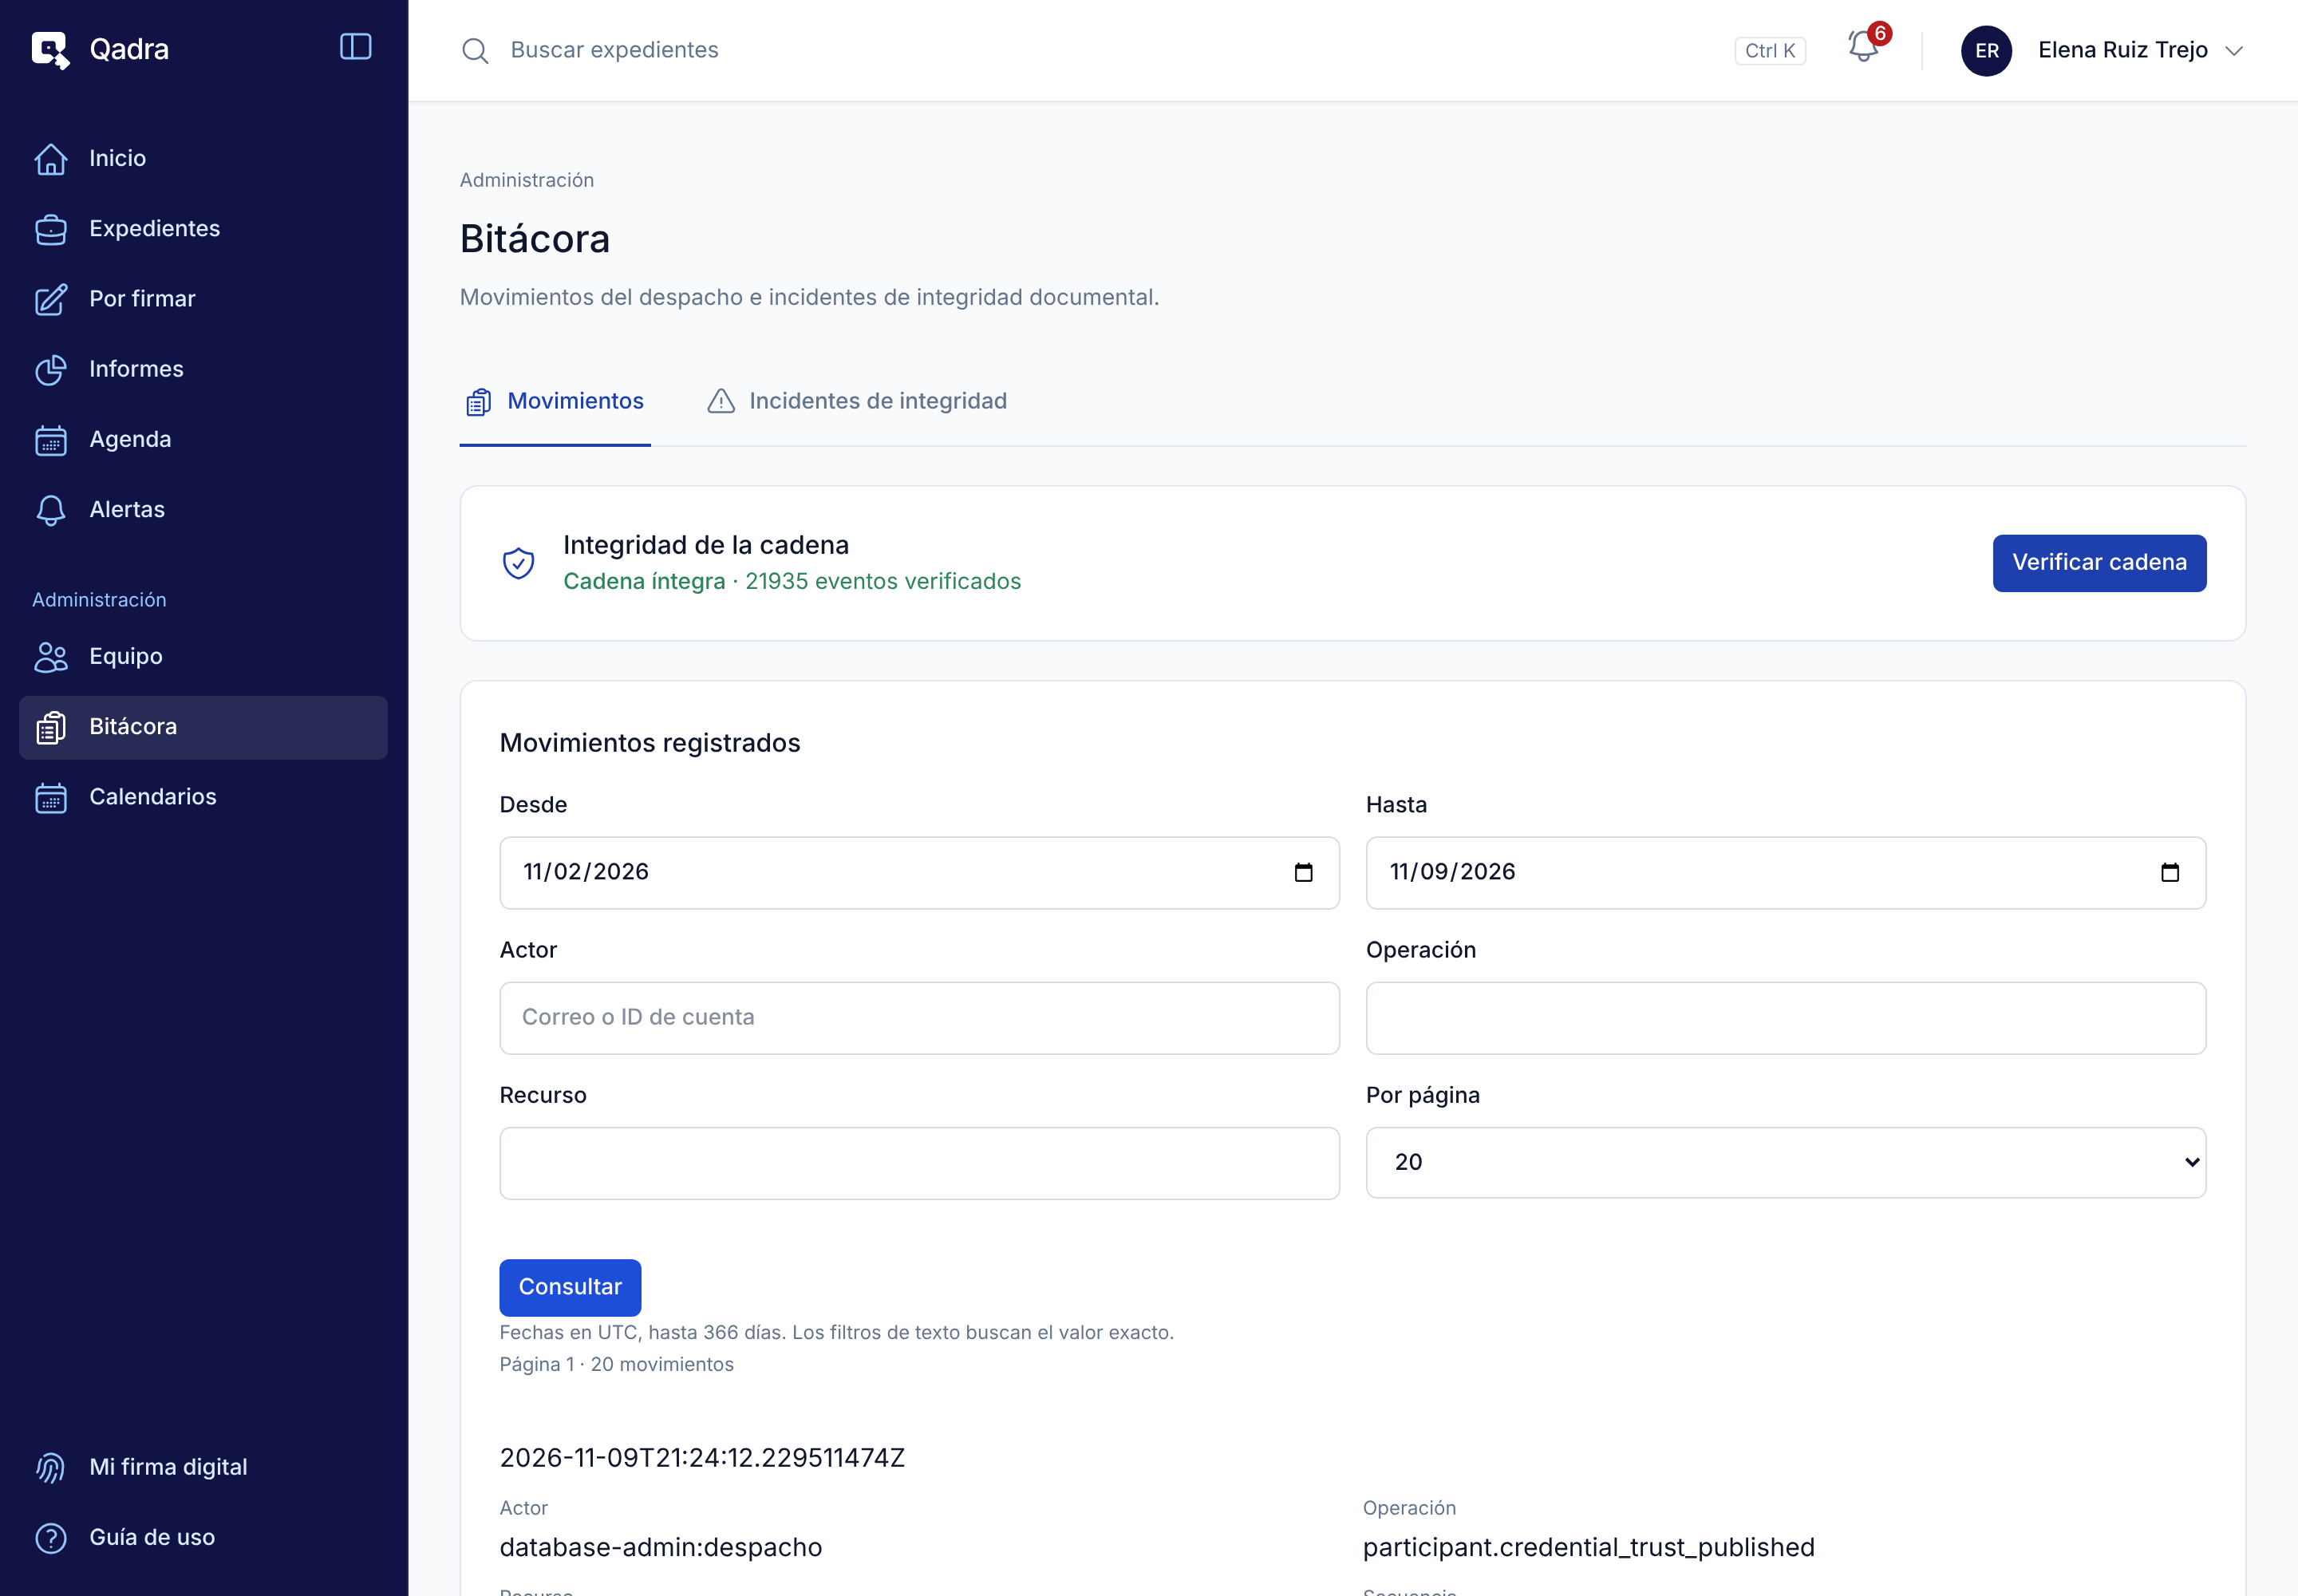
\includegraphics[width=0.9\textwidth]{capturas/A-48-bitacora.png}
  \caption{Bitácora del despacho.}
  \label{fig:manual-bitacora}
\end{figure}

\resultado Aparece \textbf{Cadena íntegra} con el número de eventos
verificados, y la lista de movimientos del periodo.

\importante{Si aparece \textbf{Alteración detectada}, la bitácora fue
modificada fuera de Qadra. Conserve el resultado y revise el primer evento
roto antes de cualquier otra acción. Si aparece el aviso \enquote{Hay
incidentes de integridad registrados.}, haga clic en
\textbf{Consultar incidentes}: un incidente no indica su causa ni a un
responsable.}

\nota{Las fechas de la bitácora están en UTC y el periodo máximo es de 366
días. Los filtros de texto buscan el valor exacto.}

% ---------------------------------------------------------------------
\section{Calendarios jurisdiccionales}\label{sec:calendarios}

\paraque Publica los días hábiles e inhábiles de cada autoridad, que Qadra
usa para calcular plazos.

\disponible Administrador (publica, reemplaza y retira). El Litigante y el
Asistente legal los consultan desde la \textbf{Agenda}.

\pasos\ Publicar un calendario:
\begin{enumerate}
  \item En el menú, haga clic en \textbf{Calendarios} y luego en
        \textbf{Publicar calendario}.
  \item Llene el \textbf{Ámbito declarado}: título, fuero, autoridad, órgano,
        territorio y entidades.
  \item Indique la \textbf{Cobertura civil} (hasta 1096 días) y el
        \textbf{Patrón semanal expreso} de cada día.
  \item Agregue las fechas inhábiles en \textbf{Excepciones por intervalo}
        y las referencias en \textbf{Fuentes públicas declaradas}.
  \item Haga clic en \textbf{Revisar calendario} y luego en
        \textbf{Confirmar calendario}.
\end{enumerate}

\begin{figure}[H]
  \centering
  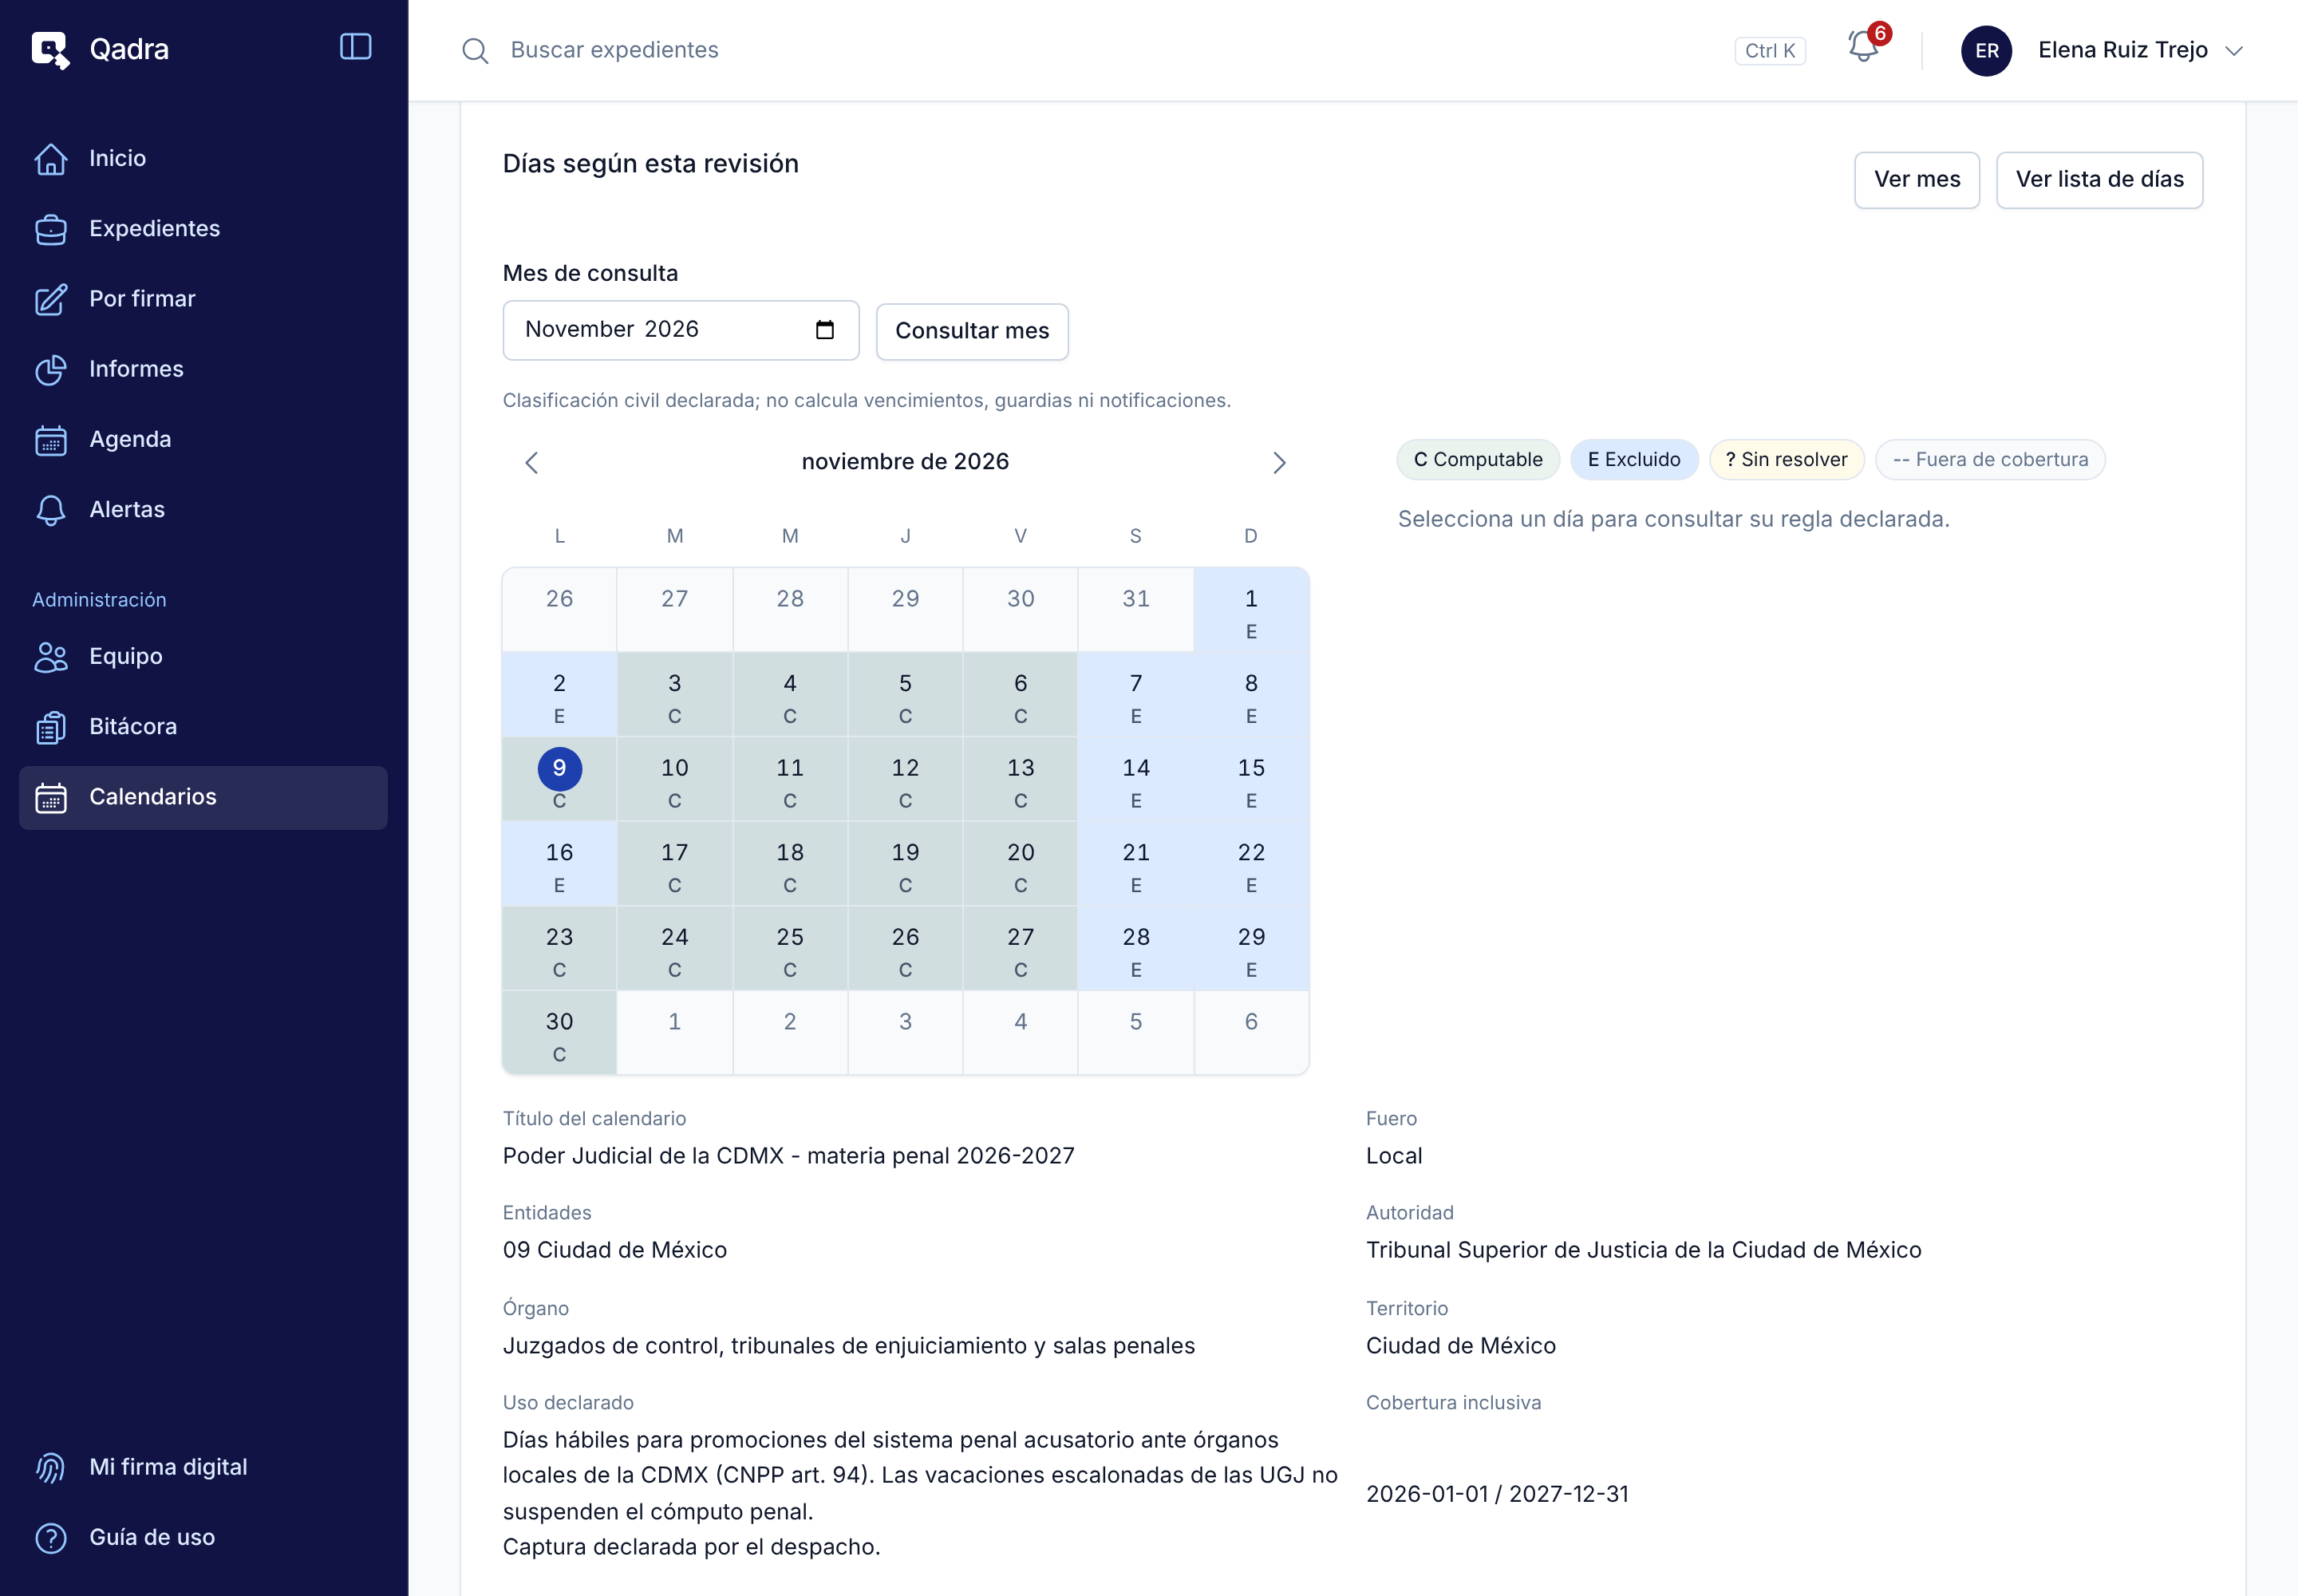
\includegraphics[width=0.9\textwidth]{capturas/A-49-calendarios.png}
  \caption{Calendarios jurisdiccionales.}
  \label{fig:manual-calendarios}
\end{figure}

\resultado Aparece \enquote{Calendario guardado con revisión y recibo.}

\begin{itemize}
  \item Para corregirlo, haga clic en \textbf{Reemplazar calendario} e
        indique el \textbf{Motivo}; la versión anterior queda en el historial.
  \item Para consultar cómo clasifica cada día, abra
        \textbf{Consultar calendario} y revise
        \textbf{Días según esta revisión}.
\end{itemize}

\importante{\textbf{Retirar calendario} es definitivo. Los plazos ya
calculados conservan su historial, pero el calendario no podrá usarse en
cálculos nuevos.}


\end{document}
